\documentclass{dissertation}
%\documentclass[print]{dissertation}
%\documentclass[print,draft]{dissertation}

\hyphenation{}
\newcommand{\sparkline}[1]{$\vcenter{\hbox{\includegraphics[scale=0.04]{#1}}}$}

\makeglossaries

\newcommand*{\origrightarrow}{}
\let\oldarrow\textrightarrow
\renewcommand*{\textrightarrow}{\fontfamily{cmr}\selectfont\origrightarrow}
\loadglsentries[main]{glossary}

\input{abbreviations}

\begin{document}

%% Specify the title and author of the thesis. This information will be used on
%% the title page (in title/title.tex) and in the metadata of the final PDF.
\title{Diversification Models and Neural Inference}
\author{Tianjian}{Qin}

%% Use Roman numerals for the page numbers of the title pages and table of
%% contents.
\frontmatter

\begin{titlepage}
\thispagestyle{empty}
\makeatletter

\begin{tikzpicture}[remember picture,overlay]

  % ---- Bottom artwork band ----
  \node[anchor=south, inner sep=0pt] at (current page.south) {%
    \includegraphics[width=\paperwidth, page=1]{title/front.pdf}%
  };

  % ---- Title block (upper third) ----
  \node[
    anchor=north,
    align=center,
    text width=0.78\paperwidth
  ] at ([yshift=-28mm]current page.north) {%

    {\CoverTitleStyle\fontsize{30}{36}\selectfont \@title\par}

    \ifx\@subtitle\undefined\else
      \vspace{0.6em}
      {\CoverSubtitleStyle\fontsize{16}{20}\selectfont \@subtitle\par}
    \fi

    \vspace{1.6em}
    {\CoverSubtitleStyle\fontsize{12}{16}\selectfont
      \@firstname\ \@lastname\par}
  };

\end{tikzpicture}

\cleardoublepage
\thispagestyle{empty}

\begin{center}

%% The following lines repeat the previous page exactly.

\vspace*{2\bigskipamount}

%% Print the title.
{\makeatletter
\titlestyle\bfseries\LARGE\@title
\makeatother}

%% Print the optional subtitle.
{\makeatletter
\ifx\@subtitle\undefined\else
    \bigskip
    \titlefont\titleshape\Large\@subtitle
\fi
\makeatother}

%% Uncomment the following lines to insert a vertically centered picture into
%% the title page.
%\vfill
%\includegraphics{title}
\vfill

%% Apart from the names and dates, the following text is dictated by the
%% promotieregelement.

{\Large\titlefont\bfseries Proefschrift}

\bigskip
\bigskip

ter verkrijging van de graad van doctor

aan de Rijksuniversiteit Groningen,

op gezag van de Rector Magnificus prof.~dr.~ir.~A.B.C~PLACEHOLDER,

voorzitter van het College voor Promoties,

in het openbaar te verdedigen

op vrijdag 99 november 2025 om 15.00 uur

\bigskip
\bigskip

door

\bigskip
\bigskip

%% Print the full name of the author.
\makeatletter
{\Large\titlefont\bfseries\@firstname\ \titleshape{\MakeUppercase{\@lastname}}}
\makeatother

\bigskip
\bigskip

Master of Science in Wetland Ecology, \\
Beijing Forestry University, China,

geboren te Chuzhou, China.

%% Extra whitespace at the bottom.
\vspace*{2\bigskipamount}

\end{center}

\clearpage
\thispagestyle{empty}

%% The following line is dictated by the promotieregelement.
\noindent Dit proefschrift is goedgekeurd door de

%% List the promotors (supervisors).
\medskip\noindent
\begin{tabular}{l}
    promotoren: Prof. dr.\ R.S.\ Etienne \\
    copromotor: Dr.\ L.L. \ Valente \\
    copromotor: Dr.\ K.J. \ van Benthem
\end{tabular}

\bigskip
\noindent Samenstelling promotiecommissie:

%% List the committee members, starting with the Rector Magnificus and the
%% promotor(s) and ending with the reserve members.
\medskip\noindent
\begin{tabular}{p{4.5cm}l}
    Rector Magnificus, & voorzitter \\
    Prof.\ dr.\ A.\ PLACEHOLDER, & Rijksuniversiteit Groningen \\
    Dr.\ A.E.\ PLACEHOLDER, & Rijksuniversiteit Groningen \\
    Dr.\ ir.\ G.\ PLACEHOLDER, & Rijksuniversiteit Groningen \\

    \medskip
    \mbox{\emph{Onafhankelijke leden:}} & \\
    Prof.\ dr.\ ir.\ A.\ PLACEHOLDER, & Rijksuniversiteit Groningen \\
    Prof. dr. P. PLACEHOLDER, & Rijksuniversiteit Groningen \\
    Dr.\ Th.\ PLACEHOLDER, & Rijksuniversiteit Groningen \\
    Prof. dr. D. PLACEHOLDER, & Rijksuniversiteit Groningen \\

    \multicolumn{2}{l}{Prof. dr. D. PLACEHOLDER has contributed to the end
    phase of writing \ldots} \\
\end{tabular}

%% Include the following disclaimer for committee members who have contributed
%% to this thesis. Its formulation is again dictated by the
%% promotieregelement.
%\medskip
%\noindent  %Prof.\ Dr.\ D.\ SOMEONE has contributed to the creation of this thesis.

\medskip
\medskip
\noindent This thesis was supported by the University of Groningen--China Scholarship Council joint scholarship program and carried out under the auspices of Groningen Institute for Evolutionary Life Sciences.

\medskip
\vfill
\begin{center}
    \includegraphics[height=0.5in]{title/logos/rug}
    \hspace{2em}
    \includegraphics[height=0.5in]{title/logos/csc}
\end{center}
\vfill

\noindent
\begin{tabular}{@{}p{0.2\textwidth}@{}p{0.8\textwidth}}
  \textit{Keywords:} & birth--death models; diversity dependence; deep learning \\[\medskipamount]
      \textit{Printed by:} &  \\[\medskipamount]
      \textit{Cover:} & Tianjian Qin \\[\medskipamount]
      \textit{Style:} & Tianjian Qin, modified from Moritz Beller \\[\medskipamount]
\end{tabular}

\medskip
\medskip
\noindent The author set this thesis in \LaTeX\xspace using the Libertinus, Inconsolata, and Noto CJK fonts.

\vspace{\bigskipamount}

% Copyrighting this is stupid, questionable, and probably illegal, because large parts of the
% thesis have already been published with the copyright resigning with the publisher.
%\noindent Copyright \textcopyright\ 2015 by A.~Einstein

%\medskip
\noindent ISBN \ldots

\medskip
\noindent An electronic version of this thesis is available at \\
\url{https://github.com/EvoLandEco/Thesis/}.

\end{titlepage}




%% The (optional) dedication can be used to thank someone or display a
%% significant quotation.
\dedication{\epigraph{To everyone who kept me going when the finish line felt far away.}{}}

\tableofcontents

\chapter*{Summary}
\addcontentsline{toc}{chapter}{Summary}
\setheader{Summary}

\dropcap{T}his thesis investigates the drivers of species diversification, and to what extent deep learning methods can recover different drivers from extant phylogenies. In particular, I focus on the effects of ecological limits (constraints to the numbers of species that can coexist) and evolutionary relatedness on speciation and extinction rates. 
First, I introduce a birth--death model, \texttt{eve}, in which speciation rates depend on both species richness and evolutionary relatedness (ER) measured at different phylogenetic scales. 
I show that tree shape and the distribution of speciation rates across lineages depend strongly on the scale at which ER acts, and that negative species richness dependence can partly mask the influence of ER on standard tree statistics. The model generates a wide range of empirically realistic, often imbalanced, phylogenies.

Second, I develop an ensemble neural-network framework for parameter estimation in diversification models. 
Combining dense, graph and recurrent neural networks trained on tree topologies, branching times and summary statistics, the method yields estimates faster than maximum-likelihood approaches and is less sensitive to tree size for constant-rate and diversity-dependent models. However, both likelihood-based and neural network estimators struggle under protracted speciation, highlighting limits imposed by the information content of trees.

Third, I use the \texttt{eve} model---which couples ecological limits with ER effects on speciation and extinction---as a testbed to map when neural networks can and cannot infer diversification mechanisms from phylogenies. 
In many cases the neural networks struggle to tell the three scenarios apart, and when the trees carry little information the estimated parameters tend to drift back toward average values. Strong global richness dependence further erodes recoverability, whereas sufficiently strong ER effects can create narrow regions of practical identifiability. Together, these results delineate the prospects and limits of using flexible diversification models and deep learning to unravel evolutionary dynamics from extant phylogenies.

\chapter*{Samenvatting}
\addcontentsline{toc}{chapter}{Samenvatting}
\setheader{Samenvatting}

{\selectlanguage{dutch}

\dropcap{I}n dit proefschrift onderzoek ik welke krachten soorten\-diversificatie sturen en in hoeverre deep-learningmethoden verschillende drijvers kunnen terugvinden uit fylogenieën van nog levende soorten. Daarbij richt ik mij vooral op het effect van ecologische grenzen (beperkingen aan het aantal soorten dat kan samenleven) en evolutionaire verwantschap op soortvormings- en uitstervingssnelheden.
Allereerst introduceer ik een geboorte--sterftemodel, \texttt{eve}, waarin soortvormingssnelheden afhangen van zowel soortrijkdom als evolutionaire verwantschap (ER), gemeten op verschillende fylogenetische schalen.
Ik laat zien dat de boomvorm en de verdeling van soortvormingssnelheden over lijnen sterk afhangen van de schaal waarop ER werkt, en dat negatieve afhankelijkheid van soortrijkdom de invloed van ER op standaard boomstatistieken deels kan maskeren. Het model genereert een breed scala aan empirisch realistische, vaak ongebalanceerde fylogenieën.

Vervolgens ontwikkel ik een ensemble-benadering met neurale netwerken voor parameterschatting in diversificatiemodellen.
Door dichte, grafische en recurrente neurale netwerken te combineren---getraind op boomtopologieën, vertakkingstijden en samenvattende statistieken---verkrijgt deze methode schattingen sneller dan maximum-likelihoodmethoden en is zij minder gevoelig voor boomgrootte bij constant-rate en diversiteitsafhankelijke modellen. Zowel likelihood-gebaseerde als neurale schatters hebben echter moeite met geprotraheerde soortvorming, wat de grenzen laat zien die worden opgelegd door de informatie-inhoud van fylogenieën.

Ten slotte gebruik ik het \texttt{eve}-model---dat ecologische grenzen koppelt aan ER-effecten op soortvorming en uitsterven---als testomgeving om in kaart te brengen wanneer neurale netwerken diversificatiemechanismen wel of niet kunnen achterhalen.
In veel gevallen hebben de neurale netwerken moeite om de drie scenario's uit elkaar te houden, en wanneer de bomen weinig informatie bevatten schuiven de geschatte parameters terug richting gemiddelde waarden. Sterke globale afhankelijkheid van soortrijkdom vermindert de herleidbaarheid verder, terwijl voldoende sterke ER-effecten smalle gebieden van praktische identificeerbaarheid kunnen creëren. Gezamenlijk schetsen deze resultaten de mogelijkheden en beperkingen van het gebruik van flexibele diversificatiemodellen en deep learning om evolutionaire dynamiek uit fylogenieën van nog levende soorten te ontrafelen.

}

\chapter*{摘要}
\addcontentsline{toc}{chapter}{摘要}
\setheader{摘要}

{\setlength{\parindent}{2em}
\noindent\dropcap{本}论文研究物种分化(由物种的形成与灭绝共同决定的过程)的驱动因素,并探讨深度学习方法是否能够仅凭现存物种的系统发育树识别这些驱动机制。论文重点关注两类影响:生态容量/生态限制(即能够共存的物种数量上限),以及物种之间的进化亲缘关系(evolutionary relatedness, ER)对物种形成与灭绝速率的效应。

首先,本文提出一个新的出生--死亡模型 \texttt{eve}。在该模型中,物种分化过程同时受到物种丰富度与进化亲缘关系(ER)的影响,并允许 ER 在不同系统发育尺度上起作用。研究表明,ER 的作用尺度会显著改变系统发育树的结构,并影响物种分化速率在谱系间的分布;同时,较强的负向丰富度依赖会在一定程度上掩盖 ER 在常用树统计量中留下的痕迹。该模型能够生成多样且与经验数据更贴近、往往高度不平衡的系统发育树。

其次,本文提出一个用于物种分化模型参数估计的集成学习框架。该框架联合使用全连接神经网络、图神经网络与循环神经网络,能够同时利用系统发育树的拓扑结构、分枝时间与汇总统计量。在应用于多种经典模型时,该方法相较最大似然估计更快,并且其估计精度对树规模的敏感性更低。然而,在“延迟物种形成”模型下,无论是最大似然方法还是神经网络方法都难以精确复原参数。这表明模型参数的可推断性往往受限于系统发育树本身所携带的信息量。

最后,本文以 \texttt{eve} 模型为检验平台,系统性评估神经网络在何种条件下能够从系统发育树中准确推断物种分化机制。结果显示,在许多情况下,神经网络难以准确区分 \texttt{eve} 模型对应的三类机制情景;当系统发育树所包含的信息量较低时,参数估计往往会回到“平均值”附近。较强的全局丰富度依赖效应会进一步削弱参数与情景的可推断性,而足够强的 ER 效应则可能在参数空间中形成狭窄但可有效识别的区域。综上所述,本论文系统讨论了深度学习框架用于物种分化模型参数估计时的表现、限制与应用前景。
}
\chapter*{Acknowledgments}
\addcontentsline{toc}{chapter}{Acknowledgments}
\setheader{Acknowledgments}

\dropcap{T}his thesis would not exist without the people who made these past years not only possible, but truly enjoyable.

First and foremost, I thank my supervisors---Rampal, Luis, and Koen. You gave me the freedom to explore, the structure to finish, and the calm reassurance to keep going when things became messy. I have learned a great deal from your clarity, standards, and generosity. Just as importantly, I am grateful that along the way you became not only my mentors, but also friends for life.

To my parents, thank you for your steady faith and encouragement, even from far away. To my wife, thank you for being my anchor---for the warmth, patience, and quiet strength that carried me through the long stretches. To my family and friends, thank you for the laughter, the check-ins, the distractions at the right moments, and for reminding me that there is a world beyond revision cycles.

I am also grateful to my colleagues at the University of Groningen and Wageningen University \& Research for the welcoming atmosphere, thoughtful conversations, and the coffee breaks that somehow turned into ideas. Working with you made research feel far less like a solitary marathon.

Finally, a special thank-you to Mitou {\color{rug-red}\faCat}, our cat, and to all the other cats who contributed in their own way---by keeping me company, insisting on timely breaks, and maintaining the firm belief that keyboards are simply deluxe pillows.

\begin{flushright}
\includegraphics[height=1.2cm, trim=10 10 10 10, clip]{acks/signature.png}\\[-0.3\baselineskip]
\textit{Groningen, the Netherlands}\\
\textit{December 2025}
\end{flushright}






%% Use Arabic numerals for the page numbers of the chapters.
\mainmatter

%% Turn on thumb indices.
\thumbtrue

%% Introduction and synthesis
\chapter{Syntroduction}
\label{syntroduction}
\blfootnote{{\color{rug-red} \faInfoCircle}~~This chapter draws in part on the introductions to the following chapters.}

\begin{fancyquotes}[font=\small\itshape]
It is interesting to contemplate an entangled bank, clothed with many plants of many kinds, with birds singing on the bushes, with various insects flitting about, and with worms crawling through the damp earth, and to reflect that these elaborately constructed forms, so different from each other, and dependent on each other in so complex a manner, have all been produced by laws acting around us.
\end{fancyquotes}

\begin{flushright}
    — Charles Darwin, \textit{On the Origin of Species} (1859)
\end{flushright}

\dropcap{C}harles Darwin's seminal work, \textit{On the Origin of Species}, published in 1859, introduced the scientific theory that populations evolve over generations through a process of natural selection. This theory was revolutionary at the time, providing a unifying explanation for the diversity of life on Earth.

Darwin proposed that individuals within a species exhibit variations in their traits, and those with characteristics better suited to their environment have higher chances of surviving and reproducing. Over successive generations, these advantageous traits become more prevalent, leading to evolutionary changes. This concept of natural selection challenged the once prevailing notion of fixed, unchanging species and suggested a common ancestry among diverse forms of life. 

Darwin’s work laid the foundation for modern evolutionary biology, influencing a wide range of scientific disciplines. By explaining how species adapt and change over time, Darwin's theory has become central to our understanding of life's \emph{complexity} and \emph{interconnectedness}. Today, these ideas are made quantitatively explicit in macroevolutionary models and phylogenetic analyses, which use branching patterns and branch lengths to study how speciation and extinction have shaped the tree of life--an endeavor at the core of this thesis.

\clearpage
\section{From Phylogenetic Trees to Networks}
\dropcap{T}ree-like diagrams for organizing knowledge predate evolutionary theory. Early examples such as Augustin Augier's 1801 ``Arbre botanique'' depicted nature's perfect, God-given order without temporal or evolutionary interpretation \citep{augier_essai_1801,hellstrom_life_2017}. In 1809, Jean-Baptiste Lamarck introduced a branching diagram in his \textit{Philosophie zoologique} that portrayed parallel lineages but did not invoke common descent \citep{lamarck_philosophie_1873}. Edward Hitchcock later published one of the first tree-like paleontological charts in 1840 \citep{archibald_edward_2009}, and Robert Chambers used a branching diagram in his 1844 \textit{Vestiges of the Natural History of Creation} to tentatively apply a tree metaphor to the history of life \citep{chambers_vestiges_1853}. By 1858, Heinrich Georg Bronn had proposed a hypothetical ``tree of life,'' yet still without a clear mechanism for evolutionary change \citep{bronn_untersuchungen_1858}.

Charles Darwin formalized the evolutionary meaning of trees in 1859 by presenting an abstract diagram with a generational scale in \textit{On the Origin of Species} (\autoref{fig::intro::darwin-tree}). This tree depicts hypothetical species evolving over a sequence of time intervals, with branching lines representing divergence, extinction, and the origin of new species. Darwin used this figure to illustrate how small, heritable differences can accumulate gradually and transform varieties into distinct species \citep{noauthor_tree_2025}. The term ``phylogeny'' itself, denoting the evolutionary relationships of species through time, was coined by Ernst Haeckel, who expanded Darwin’s concept into richly annotated trees of life \citep{mindell_tree_2013}. Haeckel’s 1866 phylogeny depicted three kingdoms---Plantae, Protista, and Animalia---and is often cited as one of the earliest comprehensive ``trees of life'' spanning multiple major lineages \citep{hossfeld_tree_2016,haeckel_generelle_1866}. His later ``Pedigree of Man'' traced all life back to Monera and placed humans at the top, reflecting a strongly hierarchical view of evolution \citep{noauthor_tree_2025}.

\begin{figure}[ht]
    \centering
    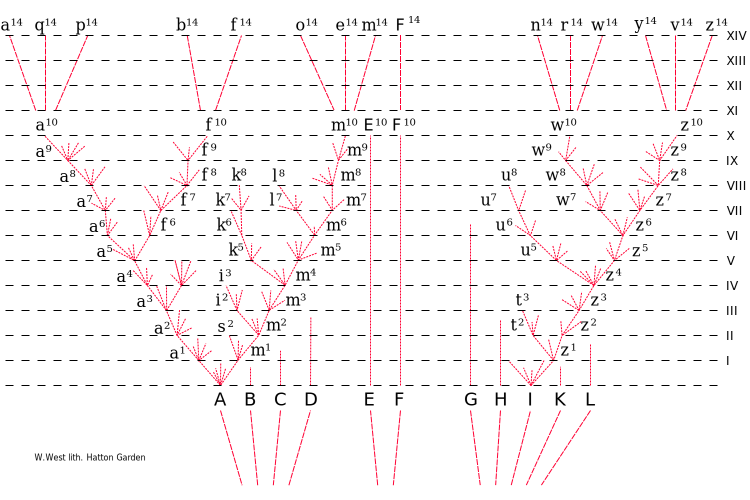
\includegraphics[width=0.90\textwidth]{introduction/darwin-tree.png}
    \caption{Darwin's abstract tree diagram illustrating evolutionary divergence over time. Modified from \textit{Inductiveload, Wikimedia Commons}.}
    \label{fig::intro::darwin-tree}
\end{figure}

\subsection{What Is a Phylogenetic Tree?}

A phylogenetic tree, or phylogeny, is a branching diagram that represents hypothesized evolutionary relationships among biological entities (e.g.\ species, populations, or genes) based on similarities and differences in their traits or genetic compositions. A typical phylogeny contains the following elements:
\begin{fancyenumerate}
    \item! \textbf{Root}: The most recent common ancestor of all entities represented in the tree.
    \item! \textbf{Branches}: Line segments representing evolutionary lineages.
    \item! \textbf{Nodes}: Points where branches join or split, typically interpreted as speciation or divergence events.
    \item! \textbf{Tips}: Terminal nodes representing the sampled taxa (extant or extinct) included in the analysis.
\end{fancyenumerate}

Trees can be \emph{rooted}, indicating a direction of time from the root to the tips, or \emph{unrooted}, which depict relationships among taxa without specifying an ancestral root. Mathematically, a phylogeny is a special case of a graph. Its topology can be rearranged visually---for example, by rotating subtrees around internal nodes or changing layout (rectangular, radial, unrooted)---without altering the underlying relationships, as long as connections among nodes are preserved (see \autoref{fig::intro::phylo-shapes}). For purely topological trees (those without meaningful branch lengths), even stretching or compressing branches does not affect the encoded relationships.

\begin{figure}[ht]
    \centering
    \resizebox{0.5\textwidth}{!}{
        \includesvg{introduction/phylo-shapes.svg}
    }
    \caption{Different layouts of the same phylogenetic tree. The blue circle marks the root, orange circles indicate internal nodes, and green circles indicate tips. Rearranging branches without changing their connections preserves the underlying topology.}
    \label{fig::intro::phylo-shapes}
\end{figure}

While phylogenies may include \emph{polytomies} (nodes with more than two descendants), they are often depicted as fully bifurcating trees. In many cases, multifurcations are treated as temporary placeholders for uncertainty that could be resolved into a series of bifurcations with additional data. Importantly, standard phylogenies are spatially implicit: they do not encode explicit geographic locations or distances.

Historically, researchers assembled phylogenies manually from morphological and anatomical comparisons. Today, phylogenies are inferred from biological data using computational methods, and they serve as the backbone for a wide variety of downstream analyses. In many molecular phylogenetic applications, trees reconstructed from extant data are treated as \emph{ultrametric}: all tips terminate at the same distance from the root and correspond to lineages observed at the present. This assumption underlies many phylogenetic algorithms and statistics.

\subsection{From Morphology and Similarity to Molecular Phylogenies}

Early phylogenetic inference relied heavily on morphology and anatomy. Researchers examined structural features of organisms to identify \emph{homologous} traits---characters inherited from a common ancestor \citep{haeckel_generelle_1866}. For example, the presence of four limbs in tetrapods is a classic homologous character. Shared homologous traits can be used to construct trees illustrating evolutionary relationships among groups (e.g.\ tetrapods in \autoref{fig::intro::homology-tree}). A major challenge in such analyses is distinguishing homologous traits from \emph{analogous} traits that evolved independently (e.g.\ wings in birds and insects), a distinction critical for accurate phylogenetic reconstruction \citep{irisarri_phylotranscriptomic_2017}.

\begin{figure}[ht]
    \centering
    \includegraphics[width=0.6\textwidth]{introduction/homology-tree.png}
    \caption{Example tree based on homologous characters (the presence of four limbs) in tetrapods. Recreated from \citet{irisarri_phylotranscriptomic_2017}.}
    \label{fig::intro::homology-tree}
\end{figure}

Phenetics, or numerical taxonomy, later emerged as a method for classifying organisms by overall similarity, often using quantitative measurements across many traits \citep{sokal_principles_1963}. The goal was to achieve objectivity by applying statistical methods to multivariate datasets, while avoiding explicit assumptions about evolutionary history. However, phenetic approaches were criticized for sometimes grouping taxa based on superficial similarity arising from convergent evolution, rather than true common ancestry \citep{de_queiroz_phenetic_1997}. Some taxonomists hoped that analyzing a sufficiently large number of characters would better cluster taxa descended from the nearest common ancestor, but this proved impractical: assembling and scoring many reliable characters was labor-intensive, and there is little guidance on which clustering or distance measures were appropriate in different situations \citep{mayr_taxonomy_2001,harvey_phylogeny_2001}.

The advent of large-scale DNA sequencing transformed phylogenetics. Molecular data allow researchers to compare DNA or protein sequences across a wide variety of organisms and to infer trees that depict their evolutionary relationships (see \autoref{fig::intro::modern-tree} for an example). These molecular phylogenies often corroborate traditional, morphology-based classifications but, in some cases, have prompted major revisions where genetic evidence reveals previously unrecognized relationships \citep{woese_towards_1990,cooper_quantitative_2003}. Fossil records play a complementary role: they provide temporal context, document extinct lineages, and offer morphological information not accessible from living taxa alone. Integrating fossil data with molecular trees enables calibration of molecular clocks and estimation of divergence times \citep{slater_integrating_2012,slater_unifying_2013,parham_best_2012}. Despite these advances, reconciling molecular and fossil evidence remains challenging due to incomplete fossil records \citep{wiens_missing_2003}, limitations on DNA preservation in ancient specimens \citep{yang_ancient_1997}, and complications from processes such as horizontal gene transfer \citep{moore_convergent_1997,kurland_horizontal_2003} and convergent evolution \citep{speed_quantification_2017,galtier_model_2007}.

\begin{figure}[ht]
    \centering
    \includegraphics[width=0.95\textwidth]{introduction/modern-tree.png}
    \caption{Example of a modern phylogeny based on DNA sequence data. Recreated from a \texttt{ggtree} illustration.}
    \label{fig::intro::modern-tree}
\end{figure}

\subsection{Alternative Tree Forms}

The classical phylogenetic tree is often presented as a strictly bifurcating hierarchy where all sampled taxa are tips, ancestors are unsampled, and evolution proceeds exclusively via splitting. In practice, several extensions of this basic model are widely used to capture more nuanced evolutionary scenarios. These include, for example, sampled ancestors \citep{morlon_reconciling_2011, slater_unifying_2013, heath_fossilized_2014, gavryushkina_bayesian_2014}, anagenesis \citep{wagner_probabilistic_2010, marshall_using_2019}, and polytomies \citep{maddison_reconstructing_1989, purvis_polytomies_1993, page_molecular_2009, drummond_bayesian_2015}.

Phylogenies can explicitly incorporate fossil taxa, often scored for morphological characters, alongside extant species. Rather than using fossils only as node calibrations, \emph{tip-dating} and \emph{total-evidence} approaches treat fossil species as tips with known ages and integrate them into the branching process \citep{slater_integrating_2012,parham_best_2012}. In these frameworks, both morphological and molecular characters contribute to the inference of topology and divergence times, and fossils may act as sampled ancestors. Including fossil taxa can break up long branches, reveal stem lineages leading to modern clades, and substantially alter interpretations of trait evolution and biogeography \citep{morlon_reconciling_2011,wiens_missing_2003}. Trees that integrate fossils in this way provide a more explicit, time-aware view of macroevolutionary history.

\subsection{Branch Lengths, Molecular Clocks, and Tree Types}

Before interpreting phylogenetic tree properties or attempting to extract quantitative information from a tree, it is essential to understand what branch lengths represent in a given case. Three broad categories are commonly distinguished (see \autoref{fig::intro::types-branch-length}):

\begin{fancyenumerate}
    \item! \textbf{Cladogram}: branch lengths carry no quantitative meaning; only the branching order matters.
    \item! \textbf{Phylogram}: branch lengths are proportional to the amount of genetic change (e.g.\ expected substitutions per site).
    \item! \textbf{Chronogram}: branch lengths are proportional to time, so that the path length from root to a tip reflects elapsed evolutionary time.
\end{fancyenumerate}

\begin{figure}[ht]
    \centering
    \includegraphics[width=0.95\textwidth]{introduction/types-branch-length.png}
    \caption{Three types of trees with different interpretations of branch length, adapted from Kellis \textit{et al.} \citep{kellis_computational_2020}. \textbf{Left:} a cladogram with no meaningful branch lengths. \textbf{Middle:} a phylogram in which branch lengths represent genetic change since divergence. \textbf{Right:} a chronogram (ultrametric tree) in which branch lengths represent time since divergence. All three trees share identical topology.}
    \label{fig::intro::types-branch-length}
\end{figure}

The classical molecular clock hypothesis assumes that genetic change accumulates at a roughly constant rate, so that branch lengths in a phylogram are proportional to divergence times when appropriately scaled \citep{robinson_molecular_2001}. Empirical studies, however, show that rates vary widely across lineages. Factors such as metabolic rate \citep{gillooly_metabolic_2004}, generation time \citep{fu_estimating_2001}, and environmental conditions \citep{bromham_exploring_2015,liu_yeast_2019} all influence substitution rates. Applying a single, global clock across distantly related taxa can therefore lead to inaccurate divergence time estimates.

To accommodate rate variation, a range of \emph{local}, \emph{discrete}, and \emph{relaxed} clock models have been developed. These allow rates to differ among branches or among clades while still linking molecular change to time \citep{lepage_general_2007,baele_accurate_2013,ho_molecular-clock_2014}. More flexible ``mixed'' branch-length models also allow for site-specific rate variation across the genome, improving both phylogeny inference and divergence-time estimation \citep{kolaczkowski_mixed_2008}. When comparing phylogenetic metrics across trees, it is crucial to account for these differences: the same statistic may have different interpretations on a cladogram, a phylogram, or a chronogram.

\subsection{What We Can Learn from Phylogenies}

Many of the hardest questions in evolution are hard because the past is unobserved: we do not directly see historical speciation, extinction, or the tempo of trait change. For many clades (especially those lacking a rich fossil record), the most information-rich record we often have is a phylogeny of extant taxa, which encodes both branching order and the timing of divergences. For example, when a novel pathogen spreads, time-calibrated phylogenies built from genome sequences can be used to reconstruct introductions, identify transmission clusters, and estimate how rapidly an epidemic is growing \citep{grenfell_unifying_2004,pybus_evolutionary_2009,stadler_birthdeath_2013}. In conservation, tree-based measures such as phylogenetic diversity and evolutionary distinctiveness help prioritize areas or lineages that represent disproportionate amounts of unique evolutionary history \citep{faith_conservation_1992,isaac_mammals_2007}. In community ecology and invasion biology, the phylogenetic structure of assemblages (clustering vs.\ overdispersion) is often used as a proxy for shared traits and niche similarity, informing hypotheses about environmental filtering, competition, and biotic resistance \citep{webb_exploring_2000,webb_phylogenies_2002,strauss_exotic_2006}.

These examples share a common logic: branching patterns summarize shared ancestry, while branch lengths carry information about the timing (or amount) of change. Phylogenies are therefore not merely static pictures of history; they are quantitative objects from which we can extract information about trait evolution, diversification dynamics, and community structure. Two broad classes of tools are especially important: phylogenetic comparative methods and tree summary statistics.

\subsubsection{Phylogenetic Comparative Methods}

Phylogenetic comparative methods use the shared evolutionary history encoded in a tree to test hypotheses about trait evolution while accounting for the non-independence of species. A foundational contribution is Felsenstein’s method of \emph{phylogenetically independent contrasts}, which transforms trait data on a tree into a set of contrasts that are statistically independent under a Brownian-motion model \citep{felsenstein_phylogenies_1985}. These contrasts can then be analyzed using standard regression or correlation techniques, while controlling for phylogenetic relatedness \citep{stadler_decoding_2024}.

Generalized least squares and related approaches extend this framework by explicitly modeling the covariance structure among species as a function of the tree and an evolutionary model \citep{rzhetsky_statistical_1992,symonds_primer_2014}. This allows hypothesis testing about processes such as adaptive evolution, constraint, or niche conservatism. Recent developments have pushed comparative methods into the high-dimensional regime. Penalized likelihood and Bayesian frameworks can accommodate many traits simultaneously and regularize complex models, enabling studies of multivariate trait evolution \citep{clavel_penalized_2019,adams_multivariate_2018,fuentes-g_bayesian_2020}.

\subsubsection{Tree Summary Statistics}

A large family of summary statistics has been proposed to quantify different aspects of tree shape, size, and timing (see \citep{janzen_phylogenetic_2024} for an overview). Although this thesis will discuss model-specific statistics later, it is useful here to highlight four broad classes:

\begin{fancyenumerate}
    \item! \textbf{Tree balance metrics}: These quantify how evenly lineages branch across the tree. Classical examples include the Sackin index, which sums the depths of all tips \citep{sackin_good_1972}, and Colless-type indices of imbalance \citep{janzen_phylogenetic_2024}. Imbalanced trees (with many short branches on one side of a split and long branches on the other) may indicate heterogeneous diversification rates or adaptive radiations.
    \item! \textbf{Branching-time statistics}: These describe the temporal pattern of divergence events. The gamma statistic, for instance, summarizes whether branching events are concentrated early or late relative to a constant-rate birth--death model \citep{pybus_testing_2000}. Deviations from the null expectation can suggest changes in diversification rates through time.
    \item! \textbf{Tree size and depth}: Simple metrics such as the number of tips (species richness) and tree height (the distance from root to most distant tip) provide basic information about the scale of the clade and the time available for diversification.
    \item! \textbf{Spectral and graph-theoretic metrics}: These approaches treat the phylogeny as a graph and summarize its structure via the eigenvalues of matrices such as the (distance) Laplacian or normalized Laplacian. The resulting spectral density profiles and derived statistics capture global features of connectivity and branching that are only partly reflected in classical imbalance or gamma-type metrics \citep{lewitus_characterizing_2016,chindelevitch_network_2021,janzen_phylogenetic_2024}.
\end{fancyenumerate}

The interpretation of these statistics depends strongly on what branch lengths represent (cladogram vs.\ phylogram vs.\ chronogram) and on how the tree was reconstructed. For example, comparing a gamma statistic or a Laplacian spectrum across trees inferred under different clock models or with different fossil calibrations can confound biology with methodology: apparent differences may simply reflect rescaled or redistributed branch lengths.

\subsection{Beyond Trees: Phylogenetic Networks}

The tree model implicitly assumes that lineages only split and never rejoin. However, many evolutionary processes violate this assumption. \emph{Reticulate} processes such as hybridization, introgression, horizontal gene transfer, and recombination create histories in which lineages merge as well as split (\autoref{fig::intro::tree-vs-network}). In such cases, representing evolution as a single bifurcating tree can be misleading: different genes may have different genealogies, and no single tree can capture all the relevant relationships \citep{moore_convergent_1997,kurland_horizontal_2003,huson_application_2006,galtier_model_2007}.

\begin{figure}[ht]
  \centering
  \begin{tikzpicture}[
    node distance=0.75cm,
    tip/.style={anchor=west},
    >=Stealth
  ]

  % Left panel: Tree
  \node[rug-red,font=\sffamily\bfseries\footnotesize,anchor=west] (labTree) at (-0.4,2.6) {Tree};

  % Backbone
  \coordinate (r1) at (0,2);
  \coordinate (a1) at (0.8,2);
  \coordinate (b1) at (0.8,1.2);
  \coordinate (c1) at (0.8,0.4);

  \coordinate (a1tip) at (2.2,2.4);
  \coordinate (b1tip) at (2.2,1.2);
  \coordinate (c1tip) at (2.2,0.0);

  \draw[treegray,thick]
    (r1) -- ++(-0.5,0)  % root stem
    (r1) -- (a1)
    (r1) -- (b1)
    (b1) -- (c1);

  \draw[treegray,thick]
    (a1) -- (a1tip)
    (b1) -- (b1tip)
    (c1) -- (c1tip);

  \node[tip,accentred] at (a1tip) {species A};
  \node[tip,accentred] at (b1tip) {species B};
  \node[tip,accentred] at (c1tip) {species C};

  % Axis arrow
  \draw[treegray,->,line width=0.4pt, yshift=-5] (-0.5,-0.2) -- (2.4,-0.2);
  \node[treegray,anchor=north,font=\sffamily\scriptsize, yshift=-5] at (1.0,-0.2)
    {divergence (tree-like)};

  % Right panel: Network
  \begin{scope}[xshift=6.0cm]
    \node[rug-red,font=\sffamily\bfseries\footnotesize,anchor=west] (labNet) at (-0.4,2.6) {Network};

    % Backbone tree
    \coordinate (r2) at (0,2);
    \coordinate (a2) at (0.8,2);
    \coordinate (b2) at (0.8,1.2);
    \coordinate (c2) at (0.8,0.4);

    \coordinate (a2tip) at (2.2,2.4);
    \coordinate (b2tip) at (2.2,1.2);
    \coordinate (c2tip) at (2.2,0.0);

    \draw[treegray,thick]
      (r2) -- ++(-0.5,0)
      (r2) -- (a2)
      (r2) -- (b2)
      (b2) -- (c2);

    \draw[treegray,thick]
      (a2) -- (a2tip)
      (b2) -- (b2tip)
      (c2) -- (c2tip);

    % Reticulation edge from A lineage into C lineage
    \draw[dashed,accentorange,thick,->]
      (1.4,2.2) .. controls (1.8,1.9) and (1.8,0.8) .. (1.4,0.4);

    % Tips
    \node[tip,accentred] at (a2tip) {species A};
    \node[tip,accentred] at (b2tip) {species B};
    \node[tip,accentred] at (c2tip) {species C};

    \node[accentorange,anchor=west,font=\sffamily\scriptsize, yshift=15] at (1.9,1.2)
      {gene flow / hybridization};
  \end{scope}

  \end{tikzpicture}
  \caption{From a strictly bifurcating tree (\textbf{left}) to a simple phylogenetic network (\textbf{right}) with a reticulation event connecting two lineages.}
  \label{fig::intro::tree-vs-network}
\end{figure}


Phylogenetic networks generalize trees by allowing edges that represent reticulation events \citep{huson_application_2006}. Conceptually, a phylogenetic network is a graph in which some nodes may have more than one parent, corresponding, for example, to a hybrid species with two ancestral lineages or to a genome that has acquired genes by lateral transfer. Several types of networks are commonly distinguished:

\begin{fancyenumerate}
    \item! \textbf{Implicit (split) networks}: These networks, such as neighbor-net or related methods, are largely exploratory. They visualize conflicting phylogenetic signals as cycles or boxes, without requiring that internal nodes correspond to actual ancestral taxa (\autoref{fig::intro::split-net}). Such networks are useful for highlighting data conflict or potential reticulation \citep{bryant_neighbor-net_2004, huson_application_2006}.
    \item! \textbf{Explicit (hybridization or species) networks}: These represent hypothesized evolutionary histories where some internal nodes are hybrids or result from gene flow between lineages \citep{warnow_advances_2019, solis-lemus_phylonetworks_2017, hibbins_phylogenomic_2022}. Here, nodes often have a direct biological interpretation, and reticulation edges correspond to specific evolutionary events (e.g.\ hybrid speciation in plants or introgression among closely related animals).
    \item! \textbf{Ancestral recombination graphs (ARGs)}: Widely used in population genetics, ARGs describe the genealogy of genetic segments in a recombining population. Recombination events introduce reticulation so that different parts of a genome trace back through different ancestral paths \citep{griffiths_ancestral_1997, lewanski_era_2024}.
\end{fancyenumerate}

\begin{figure}[ht]
  \centering
  \begin{tikzpicture}[
    node distance=1.4cm,
    tip/.style={circle,inner sep=1pt},
    >=Stealth
  ]

  % Background highlight for conflicting area
  \fill[pastelpink] (0.4,0.0) -- (3.0,0.0) -- (3.0,2.0) -- (0.4,2.0) -- cycle;

  % Nodes
  \node[tip] (A) at (0,1.5) {};
  \node[tip] (B) at (0,0.5) {};
  \node[tip] (C) at (3.4,1.5) {};
  \node[tip] (D) at (3.4,0.5) {};

  % Labels
  \node[accentred,anchor=east] at (A.west) {taxon A};
  \node[accentred,anchor=east] at (B.west) {taxon B};
  \node[accentred,anchor=west] at (C.east) {taxon C};
  \node[accentred,anchor=west] at (D.east) {taxon D};

  % Internal junctions for two alternative splits
  \coordinate (L1) at (0.8,1.0);
  \coordinate (R1) at (2.6,1.0);
  \coordinate (L2) at (0.8,1.8);
  \coordinate (R2) at (2.6,0.2);

  % Split 1: (A,B)|(C,D)
  \draw[treegray,thick]
    (A) -- (L1)
    (B) -- (L1)
    (C) -- (R1)
    (D) -- (R1)
    (L1) -- (R1);

  % Split 2: (A,D)|(B,C) forming the box
  \draw[accentorange,thick,dashed]
    (A) -- (L2) -- (R2) -- (D) -- cycle;

  % Annotation
  \node[rug-red,anchor=south west,font=\sffamily\footnotesize] at (0.5,2.05)
    {Conflicting splits};
  \node[treegray,anchor=north,font=\sffamily\scriptsize] at (1.7,-0.2)
    {split network (data conflict as boxes)};

  \end{tikzpicture}
  \caption{Toy split network for four taxa. Two incompatible splits form a ``box'', illustrating conflicting phylogenetic signal that cannot be represented on a single bifurcating tree.}
  \label{fig::intro::split-net}
\end{figure}


Reticulate evolution is especially prominent in microbes, where horizontal gene transfer can blur species boundaries and produce a ``web of life'' rather than a simple tree \citep{moore_convergent_1997,doolittle_phylogenetic_1999,kurland_horizontal_2003, bapteste_networks_2013}. In plants, hybridization and polyploidization are frequent and can drive rapid diversification \citep{linder_reconstructing_2004, marhold_polyploidy_2006}. Even in animals, genome-scale data have revealed pervasive introgression events (e.g.\ among hominins), challenging purely tree-like views of evolution \citep{racimo_evidence_2015,martin_interpreting_2017}. In all of these cases, networks provide a potentially more faithful qualitative model of evolutionary history than trees alone.

At the same time, networks are more complex to infer and interpret than trees, and the data requirements for confidently identifying reticulation events are substantial \citep{huson_application_2006}. For many questions, a tree remains an adequate and more parsimonious representation. A practical strategy is therefore to treat phylogenetic trees as a baseline model and to invoke network representations when there is clear evidence that simple branching is insufficient \citep{warnow_advances_2019, hibbins_phylogenomic_2022}. In this thesis, the focus will be on \emph{trees with calendar time units (chronograms)} and \emph{tree-based statistics}, while keeping in mind that many real evolutionary histories are embedded in richer, network-like structures. 

\clearpage
\section{Phylogenetic Birth--Death Models}
\dropcap{P}hylogenetic birth--death models provide a simple but powerful probabilistic framework for describing how speciation (``birth'') and extinction (``death'') events generate branching trees through time. In the classical constant-rate model, each lineage gives rise to new species at rate $\lambda$ and goes extinct at rate $\mu$, independently of other lineages and of time \citep{nee_extinction_1994,nee_reconstructed_1994,nee_birth-death_2006}. When $\lambda>\mu$, the expected number of lineages grows approximately exponentially, and in the absence of extinction ($\mu=0$) the process reduces to a pure-birth Yule model. Because empirical phylogenies often include only extant species, we typically observe a \emph{reconstructed} tree, in which extinct lineages have been pruned away. For such reconstructed trees, constant-rate birth--death theory predicts that lineage-through-time (LTT) plots---tracking the number of lineages with descendants at the present---should exhibit a characteristic upturn near the present, often called the ``pull of the present'', as illustrated in the left panel of \autoref{fig::intro::ltt} \citep{kubo_inferring_1995,nee_extinction_1994,stadler_decoding_2024}. Intuitively, this arises because lineages that survive to the present have not had enough time to go extinct, so the observed extinction rate near the present is reduced and net diversification appears to accelerate \citep{etienne_diversity-dependence_2012}.

\begin{figure}[ht]
  \centering
  \begin{tikzpicture}[
    >=Stealth,
    x=1cm,
    y=1cm
  ]

  % Left panel: constant-rate BD with extinction
  \begin{scope}
    % axes
    \draw[treegray,->] (0,0) -- (4,0) node[anchor=west] {\scriptsize time};
    \draw[treegray,->] (0,0) -- (0,3) node[anchor=south] {\scriptsize $\log$(lineages)};

    % log N(t) = a + r0 * t + b * t^3
    \draw[accentorange,thick,smooth,domain=0.2:3.5,samples=200]
      plot (\x,{0.6 + 0.15*\x + 0.018*pow(\x,3)});

    % label
    \node[gray,anchor=west,yshift=4] at (1.0,2.0)
      {\scriptsize constant-rate BD with extinction};
    \node[rug-red,font=\sffamily\bfseries\footnotesize,anchor=west,yshift=15] at (0,3.15)
      {Pull of the present};
  \end{scope}

  % Right panel: diversity-dependent BD (logistic N(t)) on log scale
  \begin{scope}[xshift=6cm]
    % axes
    \draw[treegray,->] (0,0) -- (4,0) node[anchor=west] {\scriptsize time};
    \draw[treegray,->] (0,0) -- (0,3) node[anchor=south] {\scriptsize $\log$(lineages)};

    % carrying capacity line
    \draw[treegray,dashed] (0.2,2.3) -- (3.8,2.3);
    \node[treegray,anchor=west] at (3.85,2.3) {\scriptsize $\log K$};

    % decelerating log-LTT
    \draw[accentred,thick,smooth,domain=0.2:3.5,samples=200]
      plot (\x,{2.3 - ln(1 + 7*exp(-1.0*\x))});

    % label
    \node[gray,anchor=west,yshift=-2] at (1.0,1.0)
      {\scriptsize diversity-dependent slowdown};

    \node[rug-red,font=\sffamily\bfseries\footnotesize,anchor=west,yshift=15] at (0,3.15)
      {Diversity-dependent birth--death};
  \end{scope}

  \end{tikzpicture}
  \caption{Lineage-through-time (LTT) plots. \textbf{Left}: approximate expected log LTT under a constant-rate birth--death model with extinction, where the slope increases from the net diversification rate $\lambda-\mu$ early on toward the speciation rate $\lambda$ near the present, illustrating the pull of the present. \textbf{Right}: diversity-dependent model with carrying capacity $K$, where the expected log LTT (red) gradually approaches $\log K$ (dashed line) as diversification slows down.}
  \label{fig::intro::ltt}
\end{figure}


Nonetheless, many empirical phylogenies do not meet this simple expectation. Across a wide range of clades, LTT curves instead show a \emph{slowdown} in lineage accumulation toward the present: the log-lineage count bends downward rather than upward, suggesting that net diversification has decreased over time \citep{purvis_phylogenetic_2008,phillimore_density-dependent_2008,moen_why_2014,aguilee_clade_2018}. This pattern contrasts with what constant-rate models predict and also with some fossil-based reconstructions of diversity, which often show long-term saturation or fluctuating equilibria rather than recent slowdowns \citep{etienne_diversity-dependence_2012,louca_why_2021}. Reconciling these discrepancies has motivated a variety of extensions to the basic birth--death framework.

Several classes of mechanisms can generate decelerating LTT curves \citep{moen_why_2014,stadler_decoding_2024}:

\begin{fancyenumerate}
    \item! \textbf{Time-dependent diversification rates}: Speciation and/or extinction rates may change through time due to extrinsic factors (e.g.\ climatic shifts, geological events) or intrinsic evolutionary innovations. For instance, models in which speciation rates decline monotonically through time---sometimes interpreted as decreasing ecological opportunity---can produce early bursts of diversification followed by slowdowns \citep{moen_why_2014,morlon_reconciling_2011,stadler_inferring_2011}.
    \item! \textbf{Protracted speciation}: Under protracted birth--death models, speciation is treated as a multi-stage process rather than an instantaneous event. Lineages first enter an incipient-species state and only later complete speciation, or may fail to do so and be reabsorbed \citep{etienne_prolonging_2012,rosindell_protracted_2010}. Because recently initiated speciation events are not yet counted as full species, protracted speciation reduces recent apparent diversification and counteracts the pull of the present. This process is illustrated in \autoref{fig::intro::protracted-bd}.
    \item! \textbf{Negative diversity-dependent diversification}: In diversity-dependent diversification (DDD) models, speciation rates decrease (and/or extinction rates increase) as the number of species in a clade rises. This can reflect competition for finite resources or niche space, leading to an effective carrying capacity $K$ for diversity \citep{valentine_evolutionary_1974,sepkoski_kinetic_1978,etienne_diversity-dependence_2012}. Early in a clade's history, when diversity is low, speciation proceeds nearly unhindered; as diversity approaches $K$, the net diversification rate declines and LTT curves tend to level off, as in the right panel of \autoref{fig::intro::ltt} \citep{wiens_causes_2011}.
    \item! \textbf{Incomplete and non-random sampling}: Empirical phylogenies often include only a fraction of the extant diversity \citep{pybus_testing_2000, cusimano_slowdowns_2010, hohna_inferring_2011}. Missing taxa---especially when sampling is biased toward deeper nodes and recent lineages are underrepresented---inflate terminal waiting times and can make lineage accumulation appear to slow toward the present even if diversification rates were constant \citep{cusimano_slowdowns_2010}. Interestingly, protracted speciation can be viewed as a related form of incomplete sampling: the underlying process contains incipient species, but the reconstructed tree records only completed species. Not all incipient lineages are ``observed'' as distinct taxa.
\end{fancyenumerate}

\begin{figure}[ht]
  \centering
  \begin{tikzpicture}[
    >=Stealth,
    x=0.8cm,
    y=0.8cm
  ]

  % Time axis
  \draw[treegray,->] (0,0) -- (10.5,0) node[anchor=west] {\scriptsize time};

  % Parent lineage
  \draw[treegray,thick] (1,1.0) -- (10.5,1.0);
  \node[treegray,anchor=east] at (1,1.0) {\scriptsize ancestral lineage};

  % Instantaneous speciation (reference)
  \draw[accentblue,thick] (1.4,1.0) -- (1.4,1.4);
  \draw[accentblue,thick] (1.4,1.4) -- (3.2,2.0);
  \node[accentblue,anchor=west] at (3.3,2.0) {\scriptsize instantaneous speciation};

  % Protracted speciation: incipient then good
  % Incipient branch
  \draw[accentorange,thick,dashed]
    (5.0,1.0) -- (5.7,1.4) node[pos=0.35,above right,xshift=-24] {\scriptsize incipient};
  % Transition to good species
  \draw[accentred,thick]
    (5.7,1.4) -- (7.5,2.0);
  \node[accentred,anchor=west] at (7.6,2.0) {\scriptsize completed speciation};

  % Protracted speciation: incipient then merge back
  % Incipient branch
  \draw[accentorange,thick,dashed]
    (8.0,1.0) -- (8.7,1.4) node[pos=0.35,above right,xshift=-24] {\scriptsize incipient};
  % Transition to good species
  \draw[treegray,thick,dashed]
    (8.7,1.4) -- (9.4,1.0);
    
  % Vertical markers for onset / completion
  \draw[treegray,dotted] (1.4,0) -- (1.4,1.0);
  \node[treegray,anchor=north,xshift=-10] at (1.4,0) {\scriptsize completion};
  \draw[treegray,dotted] (5.0,0) -- (5.0,1.0);
  \node[treegray,anchor=north,xshift=-4,yshift=-1] at (5.0,0) {\scriptsize onset};
  \draw[treegray,dotted] (5.7,0) -- (5.7,1.4);
  \node[treegray,anchor=north,xshift=10,yshift=-0.55] at (5.7,0) {\scriptsize completion};
  \draw[treegray,dotted] (8.0,0) -- (8.0,1.0);
  \node[treegray,anchor=north,yshift=-1] at (8.0,0) {\scriptsize onset};
  \draw[treegray,dotted] (9.4,0) -- (9.4,1.0);
  \node[treegray,anchor=north,yshift=-0.55] at (9.4,0) {\scriptsize merged};

  \end{tikzpicture}
  \caption{Illustration of protracted speciation. A new lineage enters an incipient-species stage (dashed orange) before becoming a fully recognized species (solid red), delaying the appearance of new species in reconstructed phylogenies relative to instantaneous speciation. A new lineage may fail and merge back.}
  \label{fig::intro::protracted-bd}
\end{figure}


In negative diversity-dependent models, species richness is usually treated as a single scalar state variable that summarizes competition, niche occupancy, and other ecological interactions. In practice, species act as proxies for mechanistic factors such as functional traits, ecological niches, and biotic interactions that ultimately shape ecological limits \citep{srivastava_phylogenetic_2012,kondratyeva_reconciling_2019}. This implicitly assumes that all species contribute equally to filling ecological space.

\begin{figure}[ht]
  \centering
  \begin{tikzpicture}[
    x=0.6cm,
    y=0.6cm,
    >=Stealth
  ]

  % --- Left: equivalent species ---
  \begin{scope}
    % big niche box
    \draw[accentred,dashed,thick,rounded corners]
      (0,0) rectangle (5.17,3);
    \node[accentred,anchor=south west] at (0,3.05)
      {\scriptsize total niche space};

    % identical species boxes
    \foreach \x/\y in {0.3/0.3, 1.5/0.3, 2.7/0.3, 3.9/0.3,
                       0.3/1.2, 1.5/1.2, 2.7/1.2, 3.9/1.2,
                       0.3/2.1, 1.5/2.1, 2.7/2.1, 3.9/2.1} {
      \draw[treegray,fill=pastelblue] (\x,\y) rectangle ++(1.0,0.6);
    }

    \node[treegray,anchor=north west] at (0, -0.3)
      {\scriptsize species treated as equivalent};
  \end{scope}

  % --- Right: relatedness-dependent niches ---
  \begin{scope}[xshift=4.2cm]
    % big niche box
    \draw[accentred,dashed,thick,rounded corners]
      (0,0) rectangle (5.17,3);
    \node[accentred,anchor=south west] at (0,3.05)
      {\scriptsize total niche space};

    % species with varying widths & colors
    % clade 1 (similar, close relatives)
    \draw[fill=pastelblue,draw=treegray] (0.3,0.3) rectangle ++(1.4,0.6);
    \draw[fill=pastelblue!80!accentred,draw=treegray] (1.8,0.3) rectangle ++(1.3,0.6);
    \draw[fill=pastelblue!60!accentred,draw=treegray] (3.2,0.3) rectangle ++(1.1,0.6);

    % clade 2 (different niche cluster)
    \draw[fill=pastelpink,draw=treegray] (0.4,1.4) rectangle ++(0.9,0.7);
    \draw[fill=pastelpink!90!accentorange,draw=treegray] (1.6,1.5) rectangle ++(1.6,0.6);

    % a highly distinct species
    \draw[fill=accentorange!40,draw=treegray,thick] (3.0,2.0) rectangle ++(1.8,0.8);

    % little tombstones for extinctions
    \draw[treegray,fill=treegray!10] (0.6,2.1) -- ++(0.0,0.4) -- ++(0.3,0) -- ++(0,-0.4) -- cycle;
    \draw[treegray,fill=treegray!10] (2.3,0.9) -- ++(0.0,0.4) -- ++(0.3,0) -- ++(0,-0.4) -- cycle;

    \node[treegray,anchor=north west, xshift=-5.4] at (0, -0.3)
      {\scriptsize niches structured by relatedness};
  \end{scope}

  \end{tikzpicture}
  \caption{Conceptual illustration of species non-equivalence. Left: all species are treated as equivalent units occupying similar amounts of niche space. Right: niche widths and positions differ, reflecting evolutionary relatedness and ecological similarity; closely related species cluster in niche space and may interact more strongly.}
  \label{fig::intro::niche-space-tile}
\end{figure}


Yet species may not be equivalent entities, as illustrated in \autoref{fig::intro::niche-space-tile}. Closely related species tend to share similar traits and ecological requirements due to common ancestry; they may compete more strongly, respond similarly to environmental change, or share enemies \citep{srivastava_phylogenetic_2012,helmus_phylogenetic_2007,cadotte_phylogenetic_2012,pigot_quantifying_2016}. Phylogenetic or evolutionary relatedness thus provides a convenient proxy for ecological similarity and potential interaction strength. For example, in invasion biology, species that are evolutionarily distant from the resident community can be more successful colonists, presumably because they occupy distinct niches and face less competition from close relatives \citep{zheng_species_2018,henn_environmental_2019,qin_phylogenetic_2020}. 

However, being \emph{too} distantly related may also imply a poor match to the local abiotic environment, so that environmental filtering prevents establishment even if competition is weak. This tension between reduced biotic resistance and reduced abiotic fit is one facet of Darwin’s naturalization “conundrum” and indicates that performance may peak at intermediate relatedness rather than changing monotonically \citep{gallien_contrasting_2015, ma_different_2016, park_darwins_2020}. Taken together, the impact of an additional species on diversification dynamics is very likely to hinge on \emph{how closely related} it is to other members of the clade, a concept illustrated in \autoref{fig::intro::niche-space}.

\begin{figure}[ht]
    \centering
    \includegraphics[width=0.85\textwidth]{introduction/niche-space.png}
    \caption{Species may not be equivalent entities; their traits and niche spaces can be influenced by their evolutionary relatedness. The left panel illustrates a scenario where all species are considered equivalent, with no regard for relatedness. In contrast, the right panel depicts a scenario where evolutionary relatedness affects traits and niche spaces. The phylogenetic trees in both panels are identical. Tombstone signs mark species that have gone extinct. The red dashed boxes represent the total hypothetical niche space, while the smaller colored boxes indicate the niche spaces occupied by individual species. The color gradient of these smaller boxes reflects the degree of similarity between species, and their width represents the amount of niche space each species occupies.}
    \label{fig::intro::niche-space}
\end{figure}

Most empirical and theoretical work on diversity-dependent diversification has focused on single clades and has assumed that all species within the focal clade contribute equally to limiting diversity \citep{rabosky_equilibrium_2010,etienne_diversity-dependence_2012,foote_diversity-dependent_2018}. Fewer studies have explored cross-clade or cross-lineage interactions, or explicitly distinguished between the effects of close vs.\ distant relatives \citep{pires_interactions_2017}. A recent island-frog study \citep{etienne_phylogenetic_2023} showed that diversity-dependence among closely related species had much stronger effects on colonization and diversification than interactions with more distantly related species, underscoring the importance of phylogenetic scale.

To date, few birth--death models have made evolutionary relatedness an explicit determinant of diversification rates. A natural next step is to use \emph{phylogenetic metrics} based on branch lengths---such as pairwise distances or measures of evolutionary distinctiveness---to modulate speciation and extinction rates in simulations. This is particularly appealing because most birth--death simulation algorithms produce chronograms (branch lengths proportional to time), so time since divergence is directly available and can be interpreted as a proxy for accumulated genetic and ecological differences. 

At the same time, birth--death theory reveals that the distribution of branch lengths in simulated trees can be unintuitive. For example, under a pure-birth Yule process, the expected lengths of internal and pendant branches are surprisingly similar and on average shorter than might be naively expected \citep{mooers_branch_2012}. Because many inference methods are sensitive to branch length distributions, it is crucial to be explicit about what branch lengths represent (time, amount of genetic change, or arbitrary units, as we discussed before) and how they were estimated \citep{nee_birth-death_2006,etienne_diversity-dependence_2012}. When we tie diversification rates to branch-length-based metrics, we implicitly assume that divergence time is a reasonable proxy for the accumulation of genetic and ecological differences. This assumption may hold in some systems but not in others. 

Overall, birth--death models have evolved from simple constant-rate descriptions to increasingly rich frameworks that incorporate time-dependence, diversity-dependence, protracted speciation and many more \citep{maddison_estimating_2007,fitzjohn_diversitree_2012,valente_equilibrium_2015,caetano_hidden_2018, herrera-alsina_detecting_2019}. In this thesis, we will introduce a new extension that incorporates dependence on \emph{both diversity and evolutionary relatedness}. Together, these models provide a conceptual bridge between individual-level evolutionary or ecological processes and the large-scale patterns observed in phylogenies and the fossil record. To assess their adequacy and to infer their parameters from data, we rely on a suite of statistical tools, which we discuss next.

\clearpage
\section{Inference of Diversification from Phylogenies}
\dropcap{I}nference tools play a central role in connecting birth--death models to empirical data. Given a reconstructed, time-calibrated phylogeny and, where available, fossil information, our goal is to infer diversification parameters (e.g.\ speciation and extinction rates) and to assess whether patterns such as time-dependence, diversity-dependence, or trait-dependence are supported. Time-calibrated phylogenies encode both branching times and topological relationships among species and thus provide a complementary source of information to the often incomplete fossil record \citep{kidwell_quality_1996}. When the assumed birth--death model approximates the true underlying process, it is possible to estimate speciation and extinction rates from such trees \citep{nee_reconstructed_1994,nee_inferring_2001,morlon_phylogenetic_2014}. 

\subsection{Likelihood-Based/Bayesian Methods}
Classical approaches to diversification inference rely on \emph{likelihood}-based frameworks. For a given birth--death model and parameter values, one can, in many cases, write down the probability of observing a particular reconstructed tree (or at least its ranked branching times) under that model \citep{nee_extinction_1994,nee_reconstructed_1994,stadler_simulating_2011,stadler_decoding_2024}. Maximizing this likelihood over the parameter space yields maximum likelihood estimates (MLEs) of speciation and extinction rates \citep{morlon_phylogenetic_2014,etienne_how_2016}; alternatively, embedding the likelihood in a Bayesian framework allows one to obtain posterior distributions for parameters via Markov chain Monte Carlo (MCMC) sampling \citep{xie_identifying_2023}. 

Over the past two decades, likelihood-based models have been extended in several directions. Time-varying models allow speciation and extinction rates to change as functions of time or environmental covariates \citep{morlon_reconciling_2011,stadler_inferring_2011}. Diversity-dependent models explicitly link rates to the current number of species in the clade \citep{etienne_diversity-dependence_2012,etienne_estimating_2014,valente_equilibrium_2015}. Trait-dependent or state-dependent models (e.g.\ BiSSE and its extensions) allow speciation and extinction to depend on discrete or continuous traits evolving along the tree \citep{maddison_estimating_2007,fitzjohn_diversitree_2012,alexander_quantifying_2016}. Likelihood-based methods for these models underpin many macroevolutionary analyses in the literature, and they remain the standard against which new approaches are often compared.

However, likelihood-based inference also faces important challenges. Closed-form likelihood expressions are only available for relatively simple models; more complex models can require intricate derivations or numerical approximations that are computationally expensive \citep{janzen_approximate_2015,lambert_deep_2023}. For many biologically realistic scenarios---for example, models with strong lineage heterogeneity or multiple interacting clades---deriving a tractable likelihood is prohibitively difficult. Even when a likelihood is available, identifiability issues can limit what can be learned from a single extant-only tree: different combinations of speciation and extinction rates may produce virtually indistinguishable reconstructed trees, especially when extinction is high \citep{rabosky_extinction_2010,louca_why_2021}. Small trees further exacerbate estimation bias; for example, MLEs of extinction often collapse to zero for modest-sized trees even when the true extinction rate is nonzero, whereas estimates improve as tree size (number of tips) increases \citep{etienne_how_2016}. Likelihood-based methods with many free parameters can also be prone to overfitting and may yield unstable estimates when data are limited \citep{ward_review_2008}.

\subsection{Approximate Bayesian Computation}
When likelihoods are unavailable or too costly to compute, \emph{Approximate Bayesian Computation} (ABC) offers an alternative route to parameter inference. ABC approximates the posterior distribution of parameters by (i) simulating data under proposed parameter values, (ii) summarizing both simulated and observed data by a set of summary statistics, and (iii) retaining parameter values that produce simulated statistics close to the observed ones \citep{beaumont_approximate_2002,beaumont_approximate_2010}. In principle, ABC can handle any diversification model so long as it is easy to simulate phylogenies from it.

In phylogenetics, however, applications of ABC remain relatively scarce \citep{rabosky_heritability_2009,bokma_time_2010,kutsukake_simulation-based_2013,xie_can_2023}. A central difficulty is choosing informative yet low-dimensional summary statistics that capture the relevant aspects of tree shape and branching times. Simple statistics, such as tree balance indices, the gamma statistic, or LTT-based features, may not be sufficient to distinguish between, say, time-dependent and diversity-dependent scenarios. In contrast, including many statistics can lead to a high-dimensional summary space in which ABC performs poorly. As a result, while ABC is conceptually attractive for complex birth--death models, careful design of summary statistics and distance metrics is critical and has so far limited its routine use in diversification studies \citep{xie_can_2023}.

\subsection{Machine Learning and Deep Learning Approaches}
Rapid advances in machine learning (ML)---particularly deep learning---offer new possibilities for inferring macroevolutionary parameters from phylogenetic data. Deep neural networks are function approximators that can learn complex, nonlinear relationships between inputs and outputs from large training datasets \citep{aggarwal_neural_2018}. \autoref{fig::intro::mlp} illustrates a simple example of a neural network architecture. In our context, the inputs are phylogenetic trees (or representations thereof), and the outputs are diversification parameters or model labels. Unlike classical ABC, deep learning can learn directly from high-dimensional or raw representations of trees without requiring hand-crafted summary statistics.

\begin{figure}[t]
  \centering
  \begin{tikzpicture}[
      >=stealth,
      node distance=1.2cm and 1.8cm,
      every node/.style={font=\small},
      neuron/.style={circle, draw, minimum size=10pt, inner sep=0pt},
      layerlabel/.style={font=\footnotesize\sffamily}
    ]

    % Input layer
    \foreach \i in {1,...,4} {
      \node[neuron, fill=gray!10] (I-\i) at (0, {-(\i-1)*1.0}) {};
    }
    \node[layerlabel, above=0.2cm of I-1, rug-red] {input layer};

    % Hidden layer
    \foreach \i in {1,...,5} {
      \node[neuron, fill=accentblue!10] (H-\i) at (2.3, {-(\i-1)*0.9+0.5}) {};
    }
    \node[layerlabel, above=0.2cm of H-1, rug-red] {hidden layer};

    % Output layer
    \foreach \i in {1,...,2} {
      \node[neuron, fill=red!10] (O-\i) at (4.6, {-(\i-1)*1.0-0.8}) {};
    }
    \node[layerlabel, above=0.2cm of O-1, rug-red] {output layer};

    % Connections: input to hidden
    \foreach \i in {1,...,4} {
      \foreach \j in {1,...,5} {
        \draw[->, thin] (I-\i) -- (H-\j);
      }
    }

    % Connections: hidden to output
    \foreach \i in {1,...,5} {
      \foreach \j in {1,...,2} {
        \draw[->, thin] (H-\i) -- (O-\j);
      }
    }

    % Labels for inputs/outputs
    \node[left=0.5cm of I-2] {$x_1,\dots,x_4$};
    \node[right=0.5cm of O-1] {$y_1,y_2$};

    % Legend arrow: gradient flow
    \begin{scope}[shift={(-0.2,-3.7)}]
      \draw[->, thin, gray] (1,0) -- (2,0);
      \node[font=\footnotesize, right=0.2cm] at (2,0)
        {information flow};
    \end{scope}
    
  \end{tikzpicture}
  \caption{Illustrative multi-layer perceptron with one hidden layer. Each neuron in a layer is fully connected to all neurons in the next layer, and information flows from left to right. This feed-forward architecture represents a basic building block of neural networks; deeper, convolutional, recurrent, or more complex models can all be viewed as extensions or refinements of this simple layered structure.}
  \label{fig::intro::mlp}
\end{figure}


A range of network architectures and tree representations has been explored:

\begin{fancyenumerate}
    \item! \textbf{Feature-based encodings and feed-forward networks}: One strategy is to compute vectors of tree-level features (e.g.\ branching-time summaries, balance indices, LTT-derived quantities) and feed them into standard multilayer perceptrons. This is straightforward to implement and has been used in several early applications of neural networks to phylogenetic data \citep{zhu_benchmarking_2018,lambert_deep_2023}. Its performance, however, depends heavily on the choice of features.
    \item! \textbf{Sequence encodings and recurrent neural networks}: Another approach is to serialize information about the tree, for example by ordering internal node ages from root to tips and treating the resulting sequence as a time series. Recurrent neural networks (RNNs), including LSTM and GRU variants, are designed to handle such sequential data and can therefore capture temporal dependencies in branching patterns \citep{sak_long_2014,salehinejad_recent_2017}. This allows them to learn from the ordered history of diversification events rather than from aggregated summaries.
    \item! \textbf{Graph-based representations and graph neural networks}: Because phylogenies are graph-structured, graph neural networks (GNNs) offer an attractive way to process them directly. In GNNs, each node (e.g.\ a speciation event or species) aggregates information from its neighbors over multiple message-passing layers, yielding a learned representation of the entire tree that can be used for parameter prediction \citep{kipf_semi-supervised_2016,ying_hierarchical_2018,li_deepergcn_2020,rampasek_recipe_2022, lajaaiti_comparison_2023}. This avoids discarding structural information but requires careful design of node and edge features.
    \item! \textbf{Topology-aware vectorizations and convolutional networks}: Recently, compact bijective encodings or ladderized vectorizations of trees have been proposed, which map each tree to a fixed-length vector or matrix encoding both topology and branch lengths. Convolutional neural networks (CNNs), originally developed for image recognition, can then be applied to these encodings to detect local patterns associated with particular parameter values \citep{voznica_deep_2022,lambert_deep_2023,lajaaiti_comparison_2023,moi_reconstructing_2022,reiman_popphy-cnn_2020}. These methods can automatically learn rich summary features without manual feature engineering.
\end{fancyenumerate}

Empirical evaluations of deep learning for diversification inference are encouraging. \citet{lambert_deep_2023} trained CNN-based models on simulated phylogenies under both homogeneous birth--death and state-dependent models and found that their networks could accurately recover speciation and extinction rates, often matching or exceeding the performance of MLE while being orders of magnitude faster at prediction. Similarly, \citet{voznica_deep_2022} and \citet{reiman_popphy-cnn_2020} demonstrated that deep learning models can infer epidemiological parameters from pathogen phylogenies. \citet{lajaaiti_comparison_2023} and \citet{qin_parameter_2025} compared multiple architectures (e.g. feed-forward, CNN, GNN) and highlighted trade-offs between flexibility, data requirements, and robustness across models.

\begin{figure}[t]
  \centering
  \begin{tikzpicture}[
      >=stealth,
      node distance=1.2cm and 1.8cm,
      every node/.style={font=\small},
      neuron/.style={circle, draw, minimum size=10pt, inner sep=0pt},
      layerlabel/.style={font=\footnotesize\sffamily}
    ]

    % Input layer
    \foreach \i in {1,...,4} {
      \node[neuron, fill=gray!10] (I-\i) at (0, {-(\i-1)*1.0}) {};
    }
    \node[layerlabel, above=0.2cm of I-1, rug-red] {input layer};

    % Hidden layer
    \foreach \i in {1,...,5} {
      \node[neuron, fill=accentblue!10] (H-\i) at (2.3, {-(\i-1)*0.9+0.5}) {};
    }
    \node[layerlabel, above=0.2cm of H-1, rug-red] {hidden layer};

    % Output layer
    \foreach \i in {1,...,2} {
      \node[neuron, fill=red!10] (O-\i) at (4.6, {-(\i-1)*1.0-0.8}) {};
    }
    \node[layerlabel, above=0.2cm of O-1, rug-red] {output layer};

    % Loss node on the right
    \node[draw, rounded corners, font=\footnotesize, color=accentorange!70]
      (Loss)
      at ($ (O-1)!0.5!(O-2) + (1.6cm,0) $)
      {$\mathcal{L}$};

    % Gradient flow: hidden to input
    \foreach \i in {1,...,4} {
      \foreach \j in {1,...,5} {
        \draw[<-, dashed, thin, gray] (I-\i) -- (H-\j);
      }
    }

    % Gradient flow: output to hidden
    \foreach \i in {1,...,5} {
      \foreach \j in {1,...,2} {
        \draw[<-, dashed, thin, gray] (H-\i) -- (O-\j);
      }
    }

    % Gradient flow: loss to outputs
    \foreach \j in {1,...,2} {
      \draw[<-, dashed, thin, gray] (O-\j) -- (Loss);
    }

    % Labels for inputs/outputs
    \node[left=0.5cm of I-2] {$x_1,\dots,x_4$};
    \node[right=0.3cm of Loss] {$\hat{y}_1,\hat{y}_2$};

    % Legend arrow: gradient flow
    \begin{scope}[shift={(-0.2,-3.7)}]
      \draw[<-, dashed, thin, gray] (1,0) -- (2,0);
      \node[font=\footnotesize, right=0.2cm, color=gray] at (2,0)
        {gradient flow};
    \end{scope}

  \end{tikzpicture}
  \caption{Training view of a simple multi-layer perceptron. Dashed gray arrows indicate the flow of gradients during backpropagation: the loss $\mathcal{L}$ is computed from the output predictions and then propagated backwards through the output, hidden, and input layers to update the network parameters.}
  \label{fig::intro::mlp_backprop}
\end{figure}


Despite their promise, neural network approaches also have limitations. We must explicitly define a loss function that quantifies the discrepancy between predictions and targets and then minimize this objective using backpropagation (see \autoref{fig::intro::mlp_backprop} for an illustration) and gradient-based numerical optimization \citep{kingma_adam_2014}. Training neural networks requires large numbers of simulated trees that adequately span the parameter space, and trained models may generalize poorly to empirical data that lie outside this space \citep{qin_parameter_2025}. Uncertainty quantification is less straightforward than in Bayesian frameworks, although approaches such as Bayesian neural networks or ensemble methods can provide approximate credibility intervals \citep{blundell_weight_2015, lakshminarayanan_simple_2017}. Neural-network–based estimators are not immune to the non-identifiability issues that affect classical likelihood approaches. If different parameter combinations generate phylogenies with indistinguishable or weakly distinct patterns, then no supervised learning method---no matter how flexible---can reliably disentangle those parameters from extant trees alone.

Neural models are also less interpretable than likelihood-based ones: they can predict parameter values accurately but generally do not yield simple analytical expressions or mechanistic insight. Consequently, deep learning should be viewed as complementary to, rather than a replacement for, traditional methods. For example, neural networks can quickly explore complex models or large datasets, generating hypotheses that can then be tested more formally with likelihood-based approaches where feasible.

After all, whether we maximize a likelihood in MLE or minimize a loss for a neural network, both procedures rely on numerical optimizers navigating a potentially rugged or even non-convex objective landscape and can therefore suffer from similar issues such as sensitivity to initial values and convergence to local optima (see \autoref{fig::intro::mle}) \citep{dauphin_identifying_2014,choromanska_loss_2015}.

\begin{figure}[t]
  \centering

  % Define the log-likelihood surface
  \pgfmathdeclarefunction{LLsurf}{2}{%
    % #1 = x, #2 = y
    \pgfmathparse{%
        2.2*exp(-((#1+1.5)^2 + (#2+1)^2))      % global peak
      + 1.4*exp(-((#1-2)^2   + (#2+2)^2)/1.3)  % local peak 1
      + 1.0*exp(-((#1-2)^2   + (#2-2)^2)/0.8)  % local peak 2
    }%
  }

  \begin{tikzpicture}
    \begin{axis}[
        hide axis,
        view={60}{35},
        domain=-4:4,
        y domain=-4:4,
        samples=38,
        scale=1.2,
        z buffer=sort,
        clip=false
    ]

      % Likelihood surface
      \addplot3[
        mesh,
        draw=gray!50,      % mesh line colour
        fill=gray!10,
        shader=interp
      ]
      {LLsurf(x,y)};

      % Mark the three optima
      \addplot3[
        only marks,
        mark=*,
        mark size=1.0pt,
        color=black
      ]
      coordinates {
        (-1.5,-1.0, {LLsurf(-1.5,-1.0)}) % global optimum
        ( 2.0, 2.0, {LLsurf( 2.0, 2.0)}) % local optimum 1
        %( 2.0,-2.0, {LLsurf( 2.0,-2.0)}) % local optimum 2
      };

      \node[font=\scriptsize,anchor=south,text=rug-red,xshift=26]
        at (axis cs:-1.5,-1.0,{LLsurf(-1.5,-1.0)+0.03}) {\faFlag~global optimum};      % global

      \node[font=\scriptsize,anchor=south,text=accentorange,xshift=24.5]
        at (axis cs:2.0,2.0,{LLsurf(2.0,2.0)+0.03}) {\faFlag~local optimum};          % local

      \node[font=\footnotesize,anchor=south,color=rug-red]
        at (axis cs:-1.5,-1.0,{LLsurf(-1.5,-1.0)+0.2})
        {};
      \node[font=\footnotesize,anchor=west,color=accentorange]
        at (axis cs:2.0,2.0,{LLsurf( 2.0, 2.0)+0.15})
        {};
      \node[font=\footnotesize,anchor=west]
        at (axis cs:2.0,-2.0,{LLsurf( 2.0,-2.0)+0.15})
        {};

      % ==================================================
      % Optimization paths
      % ==================================================

      % Path 1: starting far away and climbing to the LOCAL optimum at (2,2)
      \addplot3[
        domain=0:1,
        samples=30,
        variable=\t,
        very thick,
        color=accentorange
      ]
      (
        { 3.5 - 1.5*\t },           % x(t): from 3.5 to 2.0
        { -3.0 + 5.0*\t },          % y(t): from -3.0 to 2.0
        { LLsurf(3.5 - 1.5*\t, -3.0 + 5.0*\t) }
      );

      \node[font=\footnotesize,anchor=west, text=accentorange,yshift=-7,xshift=20]
        at (axis cs:3.5,-3.0,{LLsurf(3.5,-3.0)})
        {start (bad initials)};
      \node[font=\footnotesize,anchor=west, text=accentorange]
        at (axis cs:2.0,2.0,{LLsurf(2.0,2.0)+0.4})
        {};

      % Path 2: starting in another region and reaching the GLOBAL optimum
      \addplot3[
        domain=0:1,
        samples=30,
        variable=\t,
        very thick,
        color=rug-red
      ]
      (
        { -3.5 + 2.0*\t },          % x(t): from -3.5 to -1.5
        {  3.5 - 4.5*\t },          % y(t): from  3.5 to -1.0
        { LLsurf(-3.5 + 2.0*\t, 3.5 - 4.5*\t) }
      );

      \node[font=\footnotesize,anchor=east, text=rug-red,yshift=12,xshift=42]
        at (axis cs:-3.5,3.5,{LLsurf(-3.5,3.5)})
        {start (good initials)};
      \node[font=\footnotesize,anchor=east, text=rug-red]
        at (axis cs:-1.5,-1.0,{LLsurf(-1.5,-1.0)+0.4})
        {};

      % Mark the two starting points of the paths
      \addplot3[
        only marks,
        mark=*,
        mark size=1.0pt,
        color=black
      ]
      coordinates {
        (3.5,-3.0,{LLsurf(3.5,-3.0)})
      };

      \addplot3[
        only marks,
        mark=*,
        mark size=1.0pt,
        color=black
      ]
      coordinates {
        (-3.5,3.5,{LLsurf(-3.5,3.5)})
      };

    \end{axis}
  \end{tikzpicture}

    \caption{Illustrative log-likelihood surface with one global optimum and two local optima. 
    The colored curves show two optimization trajectories: one (red) that gets trapped in a local maximum and one (blue) that reaches the global maximum, depending on the starting point. 
    This highlights how, for complex and multi-modal likelihood functions, gradient-based MLE can be highly sensitive to initial values and may converge to suboptimal solutions, complicating reliable parameter estimation and uncertainty assessment. 
    Training neural networks relies on similar gradient-based optimization on equally rugged loss landscapes, so deep-learning approaches to likelihood-free inference can suffer from the same issues, even though they operate on a different objective.}
    \label{fig::intro::mle}
\end{figure}


\clearpage
\section{Emerging Directions and Future Prospects}
\dropcap{R}ecent theoretical work has shown that some limitations of diversification inference are \emph{structural} rather than merely computational. Under very general birth--death formulations, extant phylogenies alone cannot uniquely identify past speciation and extinction trajectories: an infinite number of distinct rate histories can be congruent with the same reconstructed tree \citep{louca_extant_2020}. This result highlights an inherent limitation of treating a single, time-calibrated tree as the sole data object: even with infinite sequence data and perfect topology, much information about diversification histories is simply not present in the tree. A growing body of work therefore focuses on model families that are both biologically interpretable and statistically identifiable. For example, \citet{legried_class_2022,legried_identifiability_2023} demonstrate that broad classes of piecewise-constant or piecewise-polynomial birth--death models are identifiable from sufficiently large chronograms, providing guidance for rate parameterizations. In parallel, methods such as \texttt{CRABS} explore the \emph{congruence classes} of birth--death models that share the same likelihood, allowing users to summarize which qualitative features of inferred rate dynamics (e.g.\ the presence of slowdowns) are robust \citep{hohna_crabs_2022}. Together, these developments suggest that future diversification studies will increasingly rely on constrained, regularized rate models and on explicit exploration of congruent alternatives, rather than on unconstrained, highly flexible trajectories.

A second key direction is to move beyond extant timetrees as the only representation of macroevolutionary history by incorporating richer data sources. Fossil-inclusive models such as the fossilized birth--death (FBD) process jointly describe diversification, fossil sampling, and extant diversity in a single probabilistic framework \citep{heath_fossilized_2014}. By embedding fossils directly into the tree and explicitly modeling sampling, FBD-based analyses can tighten divergence-time estimates and constrain diversification rates beyond what is possible with extant-only trees. More generally, joint Bayesian frameworks that combine molecular sequences, fossils, traits, and environmental covariates offer a way to mitigate the information bottleneck inherent to trees alone \citep{silvestro_bayesian_2011,zhang_total-evidence_2016,hauffe_trait-mediated_2024,magee_locally_2020,wu_rapid_2023}. 

Moreover, as we discussed earlier, processes such as hybridization, introgression, horizontal gene transfer and recombination produce reticulate patterns of ancestry that are poorly captured by a strictly bifurcating tree \citep{huson_application_2006}. Phylogenetic networks generalize trees by allowing reticulation edges and can represent conflicting signals or non-treelike histories \citep{huson_application_2006}. Recent work argues that such networks will be increasingly important in biodiversity research, as they can capture historical connectivity and gene flow among lineages that a single tree would obscure \citep{kong_phylogenetic_2025}. In the context of diversification, network-based models remain methodologically demanding and are only beginning to be explored.

A complementary set of advances concerns \emph{inference technology} itself. On the one hand, approximate Bayesian methods based on optimization, such as variational Bayesian phylogenetic inference (VBPI), are beginning to provide scalable alternatives to Markov chain Monte Carlo for full Bayesian phylogenetics. VBPI approximates the posterior over trees and model parameters using a flexible graphical model, trained by stochastic gradient ascent \citep{zhang_variational_2024}. Extensions that incorporate normalizing flows further enrich the branch-length component of the approximation and can closely match MCMC posteriors at a fraction of the computational cost \citep{zhang_variational_2024}. On the other hand, \emph{simulation-based inference} (SBI) uses neural density estimators to learn likelihoods, posteriors or likelihood ratios directly from simulator output, without requiring closed-form likelihoods \citep{cranmer_frontier_2020}. Benchmarks across scientific domains show that state-of-the-art SBI methods based on neural likelihood or posterior estimation can be both more sample-efficient and more accurate than classical ABC, particularly in high-dimensional settings \citep{lueckmann_benchmarking_2021}. For diversification models, SBI potentially offers a promising route. Once a neural estimator has been trained on simulated trees spanning a parameter space, it can provide approximate posteriors for many empirical trees at a much lower cost.

Looking ahead, we expect progress in diversification inference to come from a \emph{joint evolution} of models, data and algorithms. Theoretical work on identifiability and congruence highlights which aspects of diversification histories can be recovered from extant trees and which require additional information. Richer data sources---including fossils, traits, spatial distributions and genomic signatures of gene flow---offer routes to overcome some of the inherent limitations of tree-based representations. Advances in machine learning, from VBPI to SBI inference, provide scalable tools for exploiting these data under increasingly complex and realistic models. 

\clearpage
\section{Scope and Structure of this Thesis}
\dropcap{T}his thesis investigates how much information about macroevolutionary diversification can be extracted from extant phylogenies when we move beyond simple, constant-rate birth--death models and combine them with modern machine learning. On the modeling side, we extend classical diversification frameworks by allowing speciation and extinction to depend not only on species richness but also on evolutionary relatedness among lineages. On the inference side, we develop and evaluate neural-network–based methods that learn from simulated trees, probing when such approaches can recover diversification parameters and mechanisms, and when potential limits in the information content of trees make this impossible. Throughout, we focus on chronograms in which branch lengths represent time, and we treat neural networks not as black-box replacements for likelihood-based inference, but as flexible tools to map out the boundaries of what can and cannot be learned from phylogenetic trees under increasingly complex birth--death models.

The main body of the thesis consists of three research chapters, each addressing a different aspect of this program:

\begin{fancyenumerate}
    \item! \textbf{Diversity, evolutionary relatedness, and tree shape.} We introduce a birth--death model (\texttt{eve}) in which speciation rates depend explicitly on measures of evolutionary relatedness between species, in addition to overall species richness. Using a suite of relatedness metrics that operate at different phylogenetic scales (from lineage-specific to clade-wide), we simulate trees and analyze how these scales influence standard tree statistics. We show that whole-tree relatedness effects generate smaller and more balanced trees, with speciation rates distributed evenly across tips, whereas lineage-specific effects yield different, often more imbalanced patterns. We also demonstrate that negative richness dependence can mask the signatures of relatedness in some statistics, and we identify combinations of richness and relatedness effects that reproduce the imbalanced trees commonly seen in empirical phylogenies.

    \item! \textbf{Neural-network estimation of diversification parameters.} We develop an ensemble deep-learning framework for likelihood-free inference of diversification parameters from time-calibrated trees. Our approach combines multiple architectures---a dense feed-forward network, a graph neural network, and a long short-term memory recurrent network---and allows the ensemble to learn simultaneously from graph-structured representations of phylogenies, their branching-time sequences, and vectors of tree-summary statistics. Using simulated trees from constant-rate, diversity-dependent, and protracted birth--death models, we compare our ensemble to classical maximum likelihood estimators and existing convolutional-network approaches. We find that the ensemble delivers estimates that are faster to compute and less sensitive to tree size than MLE in several scenarios, while matching or exceeding MLE accuracy when phylogenetic signals are strong, but that both MLE and neural methods struggle under protracted speciation. This chapter highlights both the potential and the limitations of neural networks as practical tools for parameter estimation in diversification models.

    \item! \textbf{Neural recoverability and complex diversification models.} We use the \texttt{eve} model as a testbed to examine when neural networks can recover diversification mechanisms from extant trees. Training graph neural networks and long short–term memory classifiers on simulated trees, we ask how well they can distinguish among scenarios in which diversification depends on phylogenetic diversity, evolutionary distinctiveness, or nearest–neighbor distance, and we complement this with regression networks that aim to recover the underlying parameters. By analyzing classification accuracy, probability calibration, regression errors, and their dependence on tree size and the strength and sign of richness and relatedness effects, we map out regions of parameter space where scenarios and parameters are practically recoverable, and others where trees potentially carry too little information. This chapter provides an empirical perspective on recoverability in richly parameterized diversification models and clarifies how far neural inference can be pushed before additional data or constraints become non-negligible.
\end{fancyenumerate}


%% Ch1
\chapter{Diversity, Evolutionary Relatedness, and Tree Shape}
\label{chapter1}
\blfootnote{{\color{rug-red} \faFile*[regular]}~~Qin, T., Valente, L.\textsuperscript{\dag}, \& Etienne, R.\textsuperscript{\dag} (2025).
Impact of evolutionary relatedness on species diversification and tree shape.
\emph{Journal of Theoretical Biology}~\cite{qin_impact_2025}. \textsuperscript{\dag} indicates joint senior authors.\\
{\color{rug-red} \faAward}~~Awarded the inaugural \emph{Denise Kirschner Best Student Paper Prize} (2025).}

\dropcap{S}lowdowns in lineage accumulation are often observed in phylogenies of extant species. One explanation is the presence of ecological limits to diversity and hence to diversification. Previous research has examined whether and how species richness (\acrshort{sr}) impacts diversification rates, but rarely considered the evolutionary relatedness (\acrshort{er}) between species, although \acrshort{er} can affect the degree of interaction between species, which likely sets these limits. To understand the influences of \acrshort{er} on species diversification and the interplay between \acrshort{sr} and \acrshort{er}, we present a simple birth-death model in which the speciation rate depends on the \acrshort{er}. We use different metrics of ER that operate at different scales, ranging from branch/lineage-specific to clade-wide scales. We find that the scales at which an effect of \acrshort{er} operates yield distinct patterns in various tree statistics. When \acrshort{er} operates across the whole tree, we observe smaller and more balanced trees, with speciation rates distributed more evenly across the tips than in scenarios with lineage-specific \acrshort{er} effects. Importantly, we find that negative  dependence of speciation masks the impact of \acrshort{er} on some of the tree statistics. Our model allows diverse evolutionary trajectories for producing imbalanced trees, which are commonly observed in empirical phylogenies but have been challenging to replicate with earlier models.

\clearpage
{ % Constrain counter reset
% Hacky command for displaying Appendix citations
\renewcommand{\subsectionautorefname}{Appendix}
\section{Introduction}
\label{ch1::sec::intro}
\dropcap{P}hylogenetic trees are important tools to estimate past processes that may explain the current species richness of clades, such as diversification rates. Over the last two decades, the increasing availability of DNA sequence data and of tools to reconstruct phylogenetic trees from these data has led to the development of birth-death models that use molecular phylogenies as a source of information to study diversification dynamics \citep{nee_tempo_1992,purvis_phylogenetic_2008,quental_diversity_2010,etienne_diversity-dependence_2012}. Lineage-through-time (LTT) plots, semi-logarithmic plots that track the number of lineages that have descendants at the present through time, are a powerful way of summarizing diversification dynamics. If per-lineage rates of speciation and extinction have been constant through time, the accumulation of lineages increases through time exponentially, with an even stronger increase close to the present, a phenomenon called the ‘pull-of-the-present’ \citep{nee_extinction_1994,kubo_inferring_1995}. However, a large number of empirical phylogenies display a different pattern: they often show recent deceleration \citep{purvis_phylogenetic_2008,phillimore_density-dependent_2008,moen_why_2014,aguilee_clade_2018}, which contrasts with findings from the fossil record \citep{etienne_diversity-dependence_2012,louca_why_2021}.

Several hypotheses have been put forward to explain the observed slowdowns in phylogenies of extant species \citep{moen_why_2014}, such as time-dependent speciation rate \citep{moen_why_2014}, protracted speciation \citep{etienne_prolonging_2012} and negative diversity-dependent diversification \citep{valentine_evolutionary_1974,sepkoski_kinetic_1978,etienne_diversity-dependence_2012}. In negative diversity-dependent diversification models, the speciation rate declines with increasing species diversity (\acrshort{sr}). 

Current models of diversity-dependent diversification assume that speciation rate depends on global \acrshort{sr}, regardless of evolutionary relationships of the species. The general underlying idea is that species diversification results in the occupation of available niche spaces, leaving limited opportunities for subsequent species to use those niches (\autoref{fig:figure1}), because evolving clades compete for finite ecological resources \citep{wiens_causes_2011}. In these models, \acrshort{sr} acts as a proxy for more mechanistic factors such as functional traits, niches and ecological interactions, which ultimately may influence ecological limits \citep{srivastava_phylogenetic_2012,kondratyeva_reconciling_2019}. While past ecological interactions between species are difficult to infer, useful proxies are evolutionary relatedness (\acrshort{er}) metrics, which quantify the phylogenetic distance between taxa. \acrshort{er} can represent the ecological roles of the species well \citep{helmus_phylogenetic_2007,pigot_quantifying_2016}, as closely related species are more likely to share trait states and ecological functions than distantly related species \citep{srivastava_phylogenetic_2012}, and evolutionary distance may be related to fitness and niche differences \citep{cadotte_phylogenetic_2012}, which in turn can affect speciation and extinction. Here, we may learn from insights from phylogenetic community ecology \citep{webb_phylogenies_2002, mayfield_opposing_2010, hillerislambers_rethinking_2012} and invasion biology. For example, alien species that are evolutionarily distant from those in the local community may have a greater chance of establishing \citep{zheng_species_2018}, so using \acrshort{er} as a proxy to quantify open niche spaces may explain the success of plant invaders \citep{henn_environmental_2019,qin_phylogenetic_2020}.

The potentially powerful phylogenetic proxies for ecological interactions, however, have been the subject of intense debate because the underlying assumptions are often not robustly supported \citep{gerhold_phylogenetic_2015, pigot_quantifying_2016}. Indeed, there is mixed evidence regarding the effectiveness of these proxies. On the one hand, \citet{tucker_relationship_2018} concluded that phylogenetic diversity is a useful proxy for functional diversity, because phylogenetic diversity correlates more strongly with functional diversity when trait dimension increases (multidimensional trait space), although that correlation is weakened when trait evolution models become increasingly complex. On the other hand, \citet{mazel_prioritizing_2018} found that in many cases phylogenetic diversity only poorly captures functional diversity, even less so than random selection. Furthermore, \citet{venail_species_2015} found that trait and functional variation among species is largely explained by \acrshort{sr} but not phylogenetic relatedness (a concept similar to \acrshort{er}). Recently, \citet{pie_clade_2023} found that sympatry with closely-related species does not lead to decreasing speciation rates in a variety of vertebrate clades, implying that the underlying mechanisms of diversity-dependent diversification remain unconfirmed. 

\begin{figure}[ht]
    \centering
    \includegraphics[width=0.6\textwidth]{chapter1/figure1D.png} % Relative width to the width of the main text
    \caption{Illustration of how evolutionary relatedness (\acrshort{er}) is computed within clades and species in a phylogeny, as measured by three metrics: \acrshort{pd} (phylogenetic diversity), \acrshort{ed} (evolutionary distinctiveness), and \acrshort{nnd} (nearest neighbor distance). The tree on the left represents a phylogeny with extant and extinct (marked by tombstone icons) species. The numbered axis in the middle marks the branch lengths in evolutionary time (million-years). The colored circle and squares at the tips of the phylogeny represent corresponding species. On the right of the plot, the species denoted by a gray circle, an orange square and a yellow square form a combination of high \acrshort{pd} (17), while the species denoted by the gray circle, the blue square and the yellow square form a combination of low \acrshort{pd} (13). The species with the highest \acrshort{ed} value (12) is represented by a circle, and those with lower \acrshort{ed} values (less than 12) are represented by a square. The yellow and green dashed-lines between species illustrate two pairs of species, one with a low \acrshort{nnd} value (2) and one with a high \acrshort{nnd} value (12).}
    \label{fig:figure1}
\end{figure}

While these concerns indicate that support for a role of \acrshort{er} on diversification is not clear, this may be because we do not know what signal \acrshort{er} is expected to leave in phylogenetic trees and extant communities \citep{rabosky_heritability_2009,ricklefs_evolutionary_2010,wiens_causes_2011}. Most studies have only considered diversity-dependence within clades of phylogenetically closely related species \citep{rabosky_equilibrium_2010,etienne_diversity-dependence_2012,foote_diversity-dependent_2018}, whereas only a few have considered diversity-dependence between clades of phylogenetically disparate species \citep{pires_interactions_2017}. A recent study \citep{etienne_phylogenetic_2023} using empirical data on island frogs found that a model with diversity-dependence between closely related species was preferred over one with diversity-dependence also occurring with more distantly related species, indicating that interactions of species with close relatives, but not with distant relatives, negatively affect colonization and diversification. This suggests an important role of \acrshort{er} in species diversification and the need for distinguishing between different levels of \acrshort{er} and scales at which it may have an effect on diversification. However, none of the above-mentioned studies has investigated whether \acrshort{er} directly impacts macro-evolutionary dynamics \citep{rillo_diversity-dependent_2022}. 

Assuming \acrshort{er} affects diversification rates, what signatures does this effect leave in phylogenetic trees of communities? What emergent phylogenetic patterns are expected if species facilitate or compete more strongly with their close relatives? Can phylogenetic limits imposed by \acrshort{er} be differentiated from those imposed by \acrshort{sr}? And how do \acrshort{er} effects operating at the whole clade versus more lineage-specific scales affect phylogenies? To address these questions, here we present a new phylogenetic birth-death simulation model that incorporates both \acrshort{sr} and \acrshort{er}. The model allows for positive, neutral, or negative effects of both \acrshort{sr} and \acrshort{er} on diversification rates. We measure \acrshort{er} using three different mechanisms of how \acrshort{er} can affect diversification (see Methods) each considering a different scale of the effect of \acrshort{er}. We use the new model to simulate communities under a stochastic branching process where speciation rate can vary according to \acrshort{sr} and \acrshort{er}, and analyze whether \acrshort{er} leaves a signature on the diversification dynamics by looking at various tree summary statistics. We aim to provide the first expectations for the effects of these processes on phylogenetic trees by developing a simple simulation model where the effects of \acrshort{sr} and \acrshort{er} can be studied independently or in combination. While inferring parameters from empirical datasets is beyond the scope of this study, our model presents a tool that can be used in future simulation-based parameter estimation methods, for example for generating training datasets for neural network models. Our R package ``evesim" on GitHub contains functions to generate simulated phylogenies using our model \citep{hildenbrandt_evesim_2024}.

\section{Methods}
\label{ch1::sec::methods}

\subsection{Model} 
\label{ch1::sec::methods::model}
We employed a phylogenetic stochastic model that simulates the processes of species birth and death over time \citep{nee_extinction_1994}. The model is a mechanistic process-based model that is parameterized by speciation and extinction rates along with the effect sizes of \acrshort{sr} and \acrshort{er}. It allows us to explore different evolutionary trajectories from phylogenetic trees given specific parameter settings at the start of the simulation. We assumed that all species on the same tree belong to the same clade, thus our study focuses on species diversification patterns within a clade, and the phylogenies simulated include all the extant species in the clade. We investigated different types of effects of \acrshort{er} on species diversification by considering three measures of \acrshort{er}: phylogenetic diversity (\acrshort{pd}, community-level metric), evolutionary distinctiveness (\acrshort{ed}, per-lineage metric), and nearest neighbor distance (\acrshort{nnd}, per-lineage metric). 

\acrshort{pd} measures the amount of evolutionary history represented by a group of species and is commonly used to determine how species occupy different niches \citep{tucker_relationship_2018}. We calculated \acrshort{pd} using Faith's index \citep{faith_conservation_1992}, which represents the total branch length of a phylogenetic tree reconstructed from all species in a clade. \acrshort{ed} quantifies the uniqueness of each of the species relative to other species and is a valuable tool in conservation efforts \citep{cadotte_rarest_2010}. Per species, \acrshort{ed} is defined as the sum of the pairwise distances between focal species and all other species, divided by the number of species minus one. \acrshort{nnd} also quantifies the uniqueness of a species, but only on a very local phylogenetic scale, as it is defined as the phylogenetic distance (branching length of the path) between a focal species and its nearest neighbor. \acrshort{nnd} measures the degree to which each of the species is locally clustered within specific clades, and is less sensitive to higher-level phylogenetic structures than \acrshort{ed} \citep{webb_exploring_2000}. Unlike \acrshort{pd}, which is a clade-level metric and assigns a single value for all species in the clade, \acrshort{ed} and \acrshort{nnd} are lineage-specific metrics, with each lineage assigned its own value.

There are many other choices of \acrshort{er} metrics, e.g. the "Fair Proportion" index \citep{redding_evolutionarily_2008} and the "Evo-Heritage" metric \citep{rosindell_phylogenetic_2024}. However, we aimed to use metrics that are computationally efficient.

$\lambda_i$, the speciation rate of a specific lineage $i$, is given by

\begin{equation}
\lambda_i=\operatorname{max}{\left(\lambda_0+\beta_NN+\beta_\varPhi\varPhi_i,\ 0\right)}
\label{equation:three}
\end{equation}
where $\lambda_0$ is the intrinsic speciation rate of all the lineages, $N$ is the species richness (across all lineages), $\varPhi_i$ represents \acrshort{er} (either \acrshort{pd}, \acrshort{ed} or \acrshort{nnd}) of the lineage $i$, $\beta_N$ is a coefficient to adjust the effect size of species richness on the speciation rate and $\beta_\varPhi$ is a coefficient to adjust the effect size of \acrshort{er} on the speciation rate. $\beta_N$ and $\beta_\varPhi$ can be positive, zero, or negative. We note that by negative \acrshort{er} we mean negative $\beta_\varPhi$ and thus that as species become evolutionarily less related, speciation rate decreases. Furthermore, if we set both $\beta_N$ and $\beta_\varPhi$ to zero, the model reduces to a standard birth-death model.

When using \acrshort{pd} as an \acrshort{er} metric, we assume that $\varPhi_i$ is the same for every lineage $i$, so the speciation rates of all lineages are equal. Unlike \acrshort{pd}, both \acrshort{ed} and \acrshort{nnd} are calculated separately for every lineage.

To account for the strong correlation between phylogenetic diversity and time when using \acrshort{pd}, we included an offset method in our model to compensate for the inflation of branch lengths in the phylogenetic tree. The method subtracts the tree age $t$ from $\varPhi_t$, which is the phylogenetic diversity at time $t$. The adjusted $\varPhi_t^\prime$ is then given by

\begin{equation}
\varPhi_t^\prime=\varPhi_t-t.
\label{equation:two}
\end{equation}

We assumed that the extinction rate $\mu$ is fixed to the intrinsic rate of extinction which is constant through time and across lineages:

\begin{equation}
{\mu=\mu}_0.
\label{equation:four}
\end{equation}

\subsection{Simulations}
\label{ch1::sec::methods::simulation}

\begin{figure}[ht]
    \centering
    \includegraphics[width=0.95\textwidth]{chapter1/figure2C.png} % Relative width to the width of the main text
    \caption{Illustration representing a stochastic simulation under the assumptions of positive speciation and extinction rates alongside a negative coefficient of evolutionary relatedness, exemplified through a scenario where phylogenetic diversity (\acrshort{pd}, left panel) or evolutionary distinctiveness (\acrshort{ed}, right panel) or nearest neighbor distance (\acrshort{nnd}, also right panel) acts as clade-wide (\acrshort{pd}) or lineage-specific (\acrshort{ed} and \acrshort{nnd}) constraint. Although ED and NND scenarios are illustrated in the same panel, the underlying processes are different. Two event types are depicted: speciation (solid gray circles) and extinction (tombstone symbols). During a speciation event, a lineage at a tree tip bifurcates into two lineages (e.g., $E_0$, $E_1$ and $E_3$). An extinction event marks a species as extinct (e.g., $E_2$). In the left panel, the branch color transition from red to blue signifies the variation in the speciation rate of lineages along \acrshort{pd}. In the right panel, the branch color transition from red to blue or green signifies the variation of per-lineage speciation rates within the phylogeny due to lineage specific (\acrshort{ed} or \acrshort{nnd}) phylogenetic diversity-dependence. The simulation unfolds as follows: it initiates from $E_0$ with two ancestral lineages $L_1$ and $L_2$, setting the initial \acrshort{pd} value to 0. Speciation rates for all extant lineages (initially $L_1$ and $L_2$) are derived from \acrshort{pd}. The first time interval, $T_0$, extends the branch lengths of $L_1$ and $L_2$. Prior to sampling event $E_1$, \acrshort{pd} is recalculated based on extant lineages, and speciation rates are updated. Event $E_1$ illustrates $L1$ bifurcating into $L_1$ and $L_3$. The subsequent time interval $T_1$ further extends the branch lengths of $L_1$, $L_2$ and $L_3$. Before sampling each event, \acrshort{pd} and speciation rates are updated. Event $E_2$ marks the extinction of $L_3$, halting its branch growth while $L_1$ and $L_2$ continue to extend through time interval $T_2$. Event $E_3$ illustrates the speciation of $L_2$ into $L_2$ and $L_4$. The final time interval, $T_3$, stops the simulation because the cumulative time ($T_0 + T_1 + T_2 + T_3$) surpasses a pre-determined time threshold, $T$. $T_3$ is then set to $T-(T_0+T_1+T_2)$. The branch lengths of $L_1$, $L_2$, and $L_4$ extend by $T_3$, marking the simulation endpoint.}
    \label{fig:figure2}
\end{figure}

We ran a series of simulations of the model under different scenarios in order to investigate the effect and signature of \acrshort{er} on various phylogenetic summary statistics. We started the simulations with two ancestral lineages, setting the values of \acrshort{er} of both lineages to zero. We used the Gillespie algorithm \citep{gillespie_general_1976}, in which the waiting time between two evolutionary events is sampled from an exponential distribution with a mean equal to the inverse of the sum of the rates of all possible events. The probability of each event is proportional to its own rate relative to the sum of the rates of all possible events. 

Two types of events can occur: speciation and extinction. When a speciation event happens, a lineage at the tip of the tree bifurcates into two lineages. When an extinction event happens, a species is marked as extinct. The simulation lasts for a predetermined time, which equals the crown age of the final phylogeny. A successful simulation is conditional on survival of both crown lineages; the simulation will start over if one of the crown lineages goes extinct entirely (see \autoref{fig:figure2} for the illustration of the simulation). Our GitHub repository \texttt{eve} \citep{qin_eve_2023} contains the codebase for the current study.

\begin{table}
    \centering      
        \caption{Parameters used in the simulations}
        \begin{tabular}{@{}ll@{}}
        \toprule
        \textbf{Parameter}                   & \textbf{Value}                \\ \midrule
        Intrinsic speciation rate          & 0.4, 0.5, 0.6                 \\
        Intrinsic extinction rate          & 0, 0.1, 0.2                   \\
        Crown age                            & 6                             \\
        Coefficient species richness N ($\beta_N$)      & -0.04, -0.02, 0               \\
        Coefficient evolutionary relatedness ($\beta_\varPhi$) & -0.04, -0.02, 0, 0.001, 0.002 \\
        Evolutionary relatedness metric      & PD, ED, NND                   \\ \bottomrule
        \end{tabular}
    \label{tab:table1}
\end{table}

We simulated phylogenies using a variety of parameter combinations (see \autoref{tab:table1}). We assumed a crown age of 6 time units, which can be interpreted as 6 million years. All combinations of parameters in \autoref{tab:table1} were used, to a total of 135 combinations, and each was repeated for the three different \acrshort{er} scenarios: \acrshort{pd}, \acrshort{ed} and \acrshort{nnd}. Thus, we had a total of 405 parameter sets. For each set we simulated 100 phylogenetic trees using the Peregrine high performance computing cluster of the University of Groningen. In our preliminary tests, we increased the number of replicates from 100 to 300 and then 1000 for the fastest parameter settings, but we did not observe noticeable trend changes with the increased number of replicates. Due to hardware limitations, we retained the number of 100 for consistency across all combinations. The parameter sets were chosen such that the simulation can be finished within the time and resource limits of the cluster. Moreover, the effects of $\beta_\varPhi$ on the diversification process are inherently non-symmetrical because positive $\beta_\varPhi$ results in a positive feedback, which has a much greater influence on the final size of the phylogenies. For this reason, we kept the positive $\beta_\varPhi$ values relatively small. Typically, when setting $\lambda_0 = 0.6$, $\mu_0 = 0$, $\beta_N = 0$, and $\beta_\varPhi < -0.1$, the output phylogeny will be very small (often less than five lineages) and hence not very meaningful. If $\beta_\varPhi > 0.002$, then the resulting phylogenies will be very large (often more than 500 lineages), which creates computational problems (many simulation steps with compututionally demanding calculation of the phylogenetic metrics).

We deliberately chose a relatively simple model to assess the effect of \acrshort{er} on diversification, rather than including a variety of realistic ecological interactions linked with \acrshort{er}. It allows us to explore parameter space better, and it may facilitate future parameter estimation from phylogenies. Most importantly, it allows gaining broad generalizable insights based on the fundamental processes we are interested in (i.e., \acrshort{er} and \acrshort{sr} effects on diversification).

\subsection{Data Analysis}
\label{ch1::sec::methods::data_analysis}
Raw output from the simulations was processed using the ``eve" package into data compatible with statistics functions in other R packages. For each parameter set, the ``treestats" \citep{janzen_phylogenetic_2024} and ``eve" packages were used to calculate summary statistics for all extant trees, excluding those with only two extant lineages. The statistics chosen were the following: the \acrshort{jone} balance index \citep{lemant_robust_2022}, the Gamma statistic \citep{pybus_testing_2000}, mean branch length, mean pairwise distance (\acrshort{mpd}) \citep{webb_phylogenies_2002} and the Rogers J index of imbalance (\acrshort{rogers} hereafter) \citep{rogers_central_1996}. 

The effects of \acrshort{sr} and \acrshort{er} were measured by the values of $\beta_N$ and $\beta_\varPhi$, respectively. The effects of the scale at which the effect operates, from whole-clade, to species-specific were determined by the \acrshort{er} mechanism (one of the three \acrshort{er} measures: \acrshort{pd} (whole-clade), \acrshort{ed} (intermediate) and \acrshort{nnd} (species-specific).

\subsection{Speciation Rate Evenness}
\label{ch1::sec::methods::spec-rate-evenness}
In the \acrshort{ed} and \acrshort{nnd} scenarios, speciation rates are expected to vary between tree tips. We measured how these rates are distributed in phylogenies by adopting a concept similar to measuring species evenness in a community, but instead quantifying the evenness of speciation rates across lineages weighted by their phylogenetic distances. Each phylogeny of $n$ lineages was given by a correlation matrix $\boldsymbol{C}$ with each lineage $i$'s speciation rate represented by $\lambda_{i}\ (i=1,2,3,\ldots,n)$. The phylogenetic evenness index $E$ is then defined as

\begin{equation}
    E=\frac{\lambda\operatorname{diag}(\boldsymbol{C})^{\top}\boldsymbol{m}-\boldsymbol{m}^{\top}\boldsymbol{C}\boldsymbol{m}}{\lambda^2-\bar{\lambda_i}\lambda}
\label{equation:nine}
\end{equation}
which was originally proposed by \citet{helmus_phylogenetic_2007}. 

In the equation, $\lambda$ denotes $\text{sum}(\lambda_1,\lambda_2,\lambda_3,\ldots,\lambda_n)$ and $\bar{\lambda_i}$ denotes $\text{mean}(\lambda_1,\lambda_2,\lambda_3,\ldots,\lambda_n)$, $\operatorname{diag}(\boldsymbol{C})$ denotes a column vector comprising the diagonal elements of the correlation matrix $\boldsymbol{C}$ (see below), $\boldsymbol{m}$ denotes an $n\times1$ column vector containing values of $\lambda_i$. The value of $E$ ranges between 0 and 1. The maximum value (i.e., 1) of $E$ only occurs when speciation rates among lineages are equal and the tree is completely balanced (star-like). Values of $E$ less than 1 represent increasing unevenness of speciation rates among the lineages. $E$ is sensitive to tree topology such that trees with uniform speciation rates can have different values of evenness.

The correlation matrix $\boldsymbol{C}$ is the standardized pairwise distance matrix. Because we only consider ultrametric (no extinct lineages) and binary (fully resolved) phylogenies, $\boldsymbol{C}$ can be computed as:

\begin{equation}
    \boldsymbol{C} = \frac{2t - \boldsymbol{R}}{2t}
\label{equation:eight}
\end{equation}
where $\boldsymbol{R}$ is the pairwise distance matrix of all the lineages of the phylogeny of $n$ lineages, with $r_{ij}\ (i=1,2,3,\ldots,n;j=1,2,3,\ldots,n)$ represents the pairwise phylogenetic distance between lineage $i$ and $j$:

\begin{equation}
    \boldsymbol{R}=	\begin{bmatrix} 
	0 & r_{12} & r_{13} &  \ldots & r_{1n}  \\
	r_{21} & 0 & r_{23} &  \ldots & r_{2n}  \\
	r_{31} & r_{32} & 0  & \ldots & r_{3n}  \\
    \vdots & \vdots & \vdots & \ddots & \vdots \\
    r_{n1} & r_{n2} & r_{n3} & \ldots & 0
    \end{bmatrix}.
\label{equation:seven}
\end{equation}

As shown in \autoref{equation:eight} and \autoref{equation:seven}, all elements of $\operatorname{diag}(\boldsymbol{C})$ are equal to one, \autoref{equation:nine} can thus be simplified as:

\begin{equation}
    E=\frac{n}{n-1}(1 - \boldsymbol{m}^{\prime\top}\boldsymbol{C}\boldsymbol{m}^{\prime})
    \label{equation:ten}
\end{equation}
where $\boldsymbol{m}^{\prime} = \boldsymbol{m} / \lambda$.

Note that this simplification is only possible for ultrametric trees with $n \geq 2$, a formal proof of \autoref{equation:eight} and the derivation of \autoref{equation:ten} are provided in \autoref{ch1::sec::appendix::proof} and \autoref{ch1::sec::appendix::simplify}.

In the case of simulated data, the models and parameters are already known to differ. Testing for statistical significance between treatments is thus meaningless; the distributional changes sufficiently demonstrate the influence of the parameters. Therefore, we focused on how summary statistics vary with the strength of \acrshort{er} and \acrshort{sr} to explain the model's power and effects.

\subsection{Data Visualization}
\label{ch1::sec::methods::data_visualization}
For visualization purposes, we selected one representative tree for each tree set of 100 trees representing a single parameter set. This tree was chosen among the complete trees based on its index vector, which has the smallest mean Mahalanobis distance \citep{de_maesschalck_mahalanobis_2000} to the other trees in the same tree set (as defined in \autoref{equation:five} below). 
In order to calculate the Mahalanobis distance for each tree, we first defined the index vector for the $i$-th tree in a set of trees resulted from $k$-th parameter set, where $k$ denotes one of the parameter sets in the 405 combinations in our simulation, as

\begin{align}
\boldsymbol{v}_{i,k} &= \begin{pmatrix}
       v_\mathrm{J}^{i,k}, &
       v_\mathrm{G}^{i,k}, &
       v_\mathrm{P}^{i,k}, &
       v_\mathrm{M}^{i,k}, &
       v_\mathrm{R}^{i,k}
     \end{pmatrix}^\top
\label{equation:five}
\end{align}
where each element of $\boldsymbol{v}_{i,k}$ represents a summary statistic of the $i$-th tree in the $k$-th set. $v_\mathrm{J}^{i,k}$ denotes the \acrshort{jone} balance index, $v_\mathrm{G}^{i,k}$ denotes the \acrshort{gamma} statistic, $v_\mathrm{P}^{i,k}$ denotes \acrshort{pd}, $v_\mathrm{M}^{i,k}$ denotes the mean pairwise distance, $v_\mathrm{R}^{i,k}$ denotes the \acrshort{rogers} balance index and $\top$ denotes the transpose of vector. These five statistics were selected based on a clustering dendrogram of various summary statistics, where they were found to be less correlated and more evenly spaced than other statistics (see \autoref{ch1::sec::appendix::heatmap}). 

The Mahalanobis distance of $\boldsymbol{v}_{i,k}$ is given as

\begin{equation}
d_{\mathrm{M}}(\boldsymbol{v}_{i,k}) = \sqrt{(\boldsymbol{v}_{i,k} - \bar{\boldsymbol{v}}_k)^\top \boldsymbol{S}^{-1} (\boldsymbol{v}_{i,k} - \bar{\boldsymbol{v}}_k)}
\label{equation:six}
\end{equation}
where $\boldsymbol{v}_{i,k}$ is the index vector for the $i$-th tree of the $k$-th set. $\bar{\boldsymbol{v}}_k$ comprises five mean values of each element respectively in the index vectors in the $k$-th set, $\top$ denotes the vector transpose, $\boldsymbol{S}$ is the covariance matrix of these vectors and $\boldsymbol{S}^{-1}$ denotes the inverse of $\boldsymbol{S}$.

For each representative tree (i.e. the tree with the smallest Mahalanobis distance to the other trees), we mapped the historical speciation rates onto the tree using the ``eve" package. The variation of speciation rates along tree lineages is represented by a continuous color scale. The actual rate values corresponding to colors were calculated as mean speciation rates (mean value of speciation rates at the beginning and at the end) of the time frames between evolutionary events in a simulation.  

LTT plots were generated using the ``eve" package for each tree set by summarizing all the trees in the set and then displaying the mean LTT curve along with shading representing the confidence interval of the set. The LTT plots were based on extant species only.

\section{Results}
\label{ch1::sec::results}
\subsection{Simulation Performance}
\label{ch1::sec::results::performance}
All simulation jobs were completed within seven hours on the computing cluster, with most of the parameter sets finishing within one hour.

When extinction rates are 0 and no species richness effect is present, a deceleration in lineage accumulation is observed in the \acrshort{pd} scenario, but only when $\beta_\varPhi$ is negative, that is, higher \acrshort{er} in the communities results in lower speciation rate on all lineages (see \autoref{fig:figure3} and the animations in \autoref{ch1::sec::appendix::treestats}).

\begin{figure}[ht]
    \centering
    \includegraphics[width=1\linewidth]{chapter1/figure3B.png} % Relative width to the width of the line
    \caption{Overview of results of simulations of a pure birth process (no extinction, see \autoref{ch1::sec::appendix::treestats} for other speciation and extinction rate combinations), with dependence of speciation on evolutionary relatedness. For all parameter sets shown in the figure, the intrinsic speciation rate at the start of the simulation ($\lambda_0$) is 0.6, the intrinsic extinction rate ($\mu_0$) is 0, and the coefficient of the species richness effect ($\beta_N$) is 0. The results are grouped by rows according to varying levels of $\beta_\varPhi$ (the coefficient of the evolutionary relatedness effect). On the left, representative simulated phylogenies and associated lineage-through time (LTT) plots are shown for dependence of speciation rates on three metrics of \acrshort{er} (left - phylogenetic diversity (\acrshort{pd}), middle - evolutionary distinctiveness (\acrshort{ed}), and right - nearest neighbor distance (\acrshort{nnd}) scenario). The colors mapped onto the trees represent the values of the speciation rate for each of the lineages during simulation time. The rates increase from blue to red. The trees colored in green are cases where the speciation rate remains unchanged throughout the simulation. Blue line in the LTT plots represents lineage accumulation through time and the shaded area is the 95\% confidence interval. On the right of each row, boxplots for the corresponding summary statistics are shown: \acrshort{jone} -  J One balance index; \acrshort{gamma} - Gamma statistic; \acrshort{sr} - total number of extant lineages; \acrshort{mpd} -  mean pairwise distance; \acrshort{mbl} - the mean branch length.}
    \label{fig:figure3}
\end{figure}

\subsection{Effects of Evolutionary Relatedness}
\label{ch1::sec::results::er_localness}
We observed a hierarchical structuring in tree topology patterns, from \acrshort{pd} to \acrshort{ed} to \acrshort{nnd}. Under the \acrshort{pd} scenario, trees exhibit a higher degree of balance (interpreted from the \acrshort{jone} balance index) than in the \acrshort{ed} scenario, which in turn exhibits more balanced trees than the \acrshort{nnd} scenario. This pattern is more prominent when $\beta_\varPhi$ decreases from zero towards more negative values, that is, when \acrshort{er} reduces the speciation rates even more. As $\beta_\varPhi$ increases from negative to positive values, that is, the \acrshort{er} effect on the speciation rates transitions from a reduction to augmentation, the differences in tree balance between \acrshort{pd}, \acrshort{ed} and \acrshort{nnd} scenarios decrease, and the trees exhibit generally lower degree of balance (see the animations in \autoref{ch1::sec::appendix::animation-main} ending with J\_One). 

As $\beta_\varPhi$ increases from -0.04 to 0 (\acrshort{er} effect becomes neutral), a general decrease in the mean pairwise distances of the trees is observed. However, no substantial change occurs when $\beta_\varPhi$ shifts from 0 to positive values (i.e., a beneficial effect of \acrshort{er} on speciation). When $\beta_\varPhi$ is negative, the trees under the \acrshort{pd} scenario exhibit larger mean pairwise distances than those in the \acrshort{ed} scenario and the trees under the \acrshort{ed} scenario exhibit larger mean pairwise distances than those in the \acrshort{nnd} scenario. As $\beta_\varPhi$ increases from -0.04 to 0, the disparities in mean pairwise distances among \acrshort{pd}, \acrshort{ed}, and \acrshort{nnd} scenarios decrease (see the animations in \autoref{ch1::sec::appendix::animation-main} ending with \acrshort{mpd} and \acrshort{mbl}). The patterns of mean branch lengths across $\beta_\varPhi$ settings are similar to those of mean pairwise distances.

The distribution of internal nodes, or the concentration of speciation events, were interpreted using the \acrshort{gamma} statistic. When $\beta_\varPhi$ is negative, the speciation events in the \acrshort{pd} scenario are located more closely to the root than in the \acrshort{ed} scenario, and the events in the \acrshort{ed} scenario are closer to the root than those in the \acrshort{nnd} scenario. These differences are reduced as $\beta_\varPhi$ increases from negative values towards zero. This pattern changes as $\beta_\varPhi$ shifts from zero towards positive values, particularly when $\beta_N$ is 0. As $\beta_\varPhi$ increases from -0.04 to 0.002, the distributions of speciation events in all three scenarios change from being closer to the root to being more evenly distributed throughout the temporal range of the phylogeny (see the animations in \autoref{ch1::sec::appendix::animation-main} ending with \acrshort{gamma}). 

The trees become notably larger (more species) as $\beta_\varPhi$ increases from -0.04 to 0. This increase is minimized when $\beta_\varPhi$ increases from 0 to 0.002. When $\beta_\varPhi$ is negative, the tree sizes are generally largest in the \acrshort{nnd} scenario, second largest in the \acrshort{ed} scenario and smallest in the \acrshort{pd} scenario. This pattern does not persist when $\beta_\varPhi$ is zero or positive. The pattern is reversed when $\beta_\varPhi$ is positive, in which case the \acrshort{pd} scenario generally has the largest tree sizes and the \acrshort{nnd} scenario the smallest (see the animations in \autoref{ch1::sec::appendix::animation-main} ending with \acrshort{sr}).

Of all model parameters, $\beta_\varPhi$ has the strongest effect on the evenness of the speciation rates across lineages. In all parameter combinations, the disparities of speciation rate evenness between \acrshort{pd}, \acrshort{ed} and \acrshort{nnd} scenarios decline with increasing $\beta_\varPhi$ (see \autoref{fig:figure4}B and the animations in \autoref{ch1::sec::appendix::animation-main} ending with ERE). 

\subsection{Interaction between the Effects}
\label{ch1::sec::results::interaction_er_sr}
The effects of $\beta_\varPhi$ (for instance the degree of disparities of the statistics between \acrshort{pd}, \acrshort{ed} and \acrshort{nnd} scenarios, and the changes of the statistics along with varying $\beta_\varPhi$) appear more prominent when $\beta_N$ imposes a less pronounced (i.e. less negative) effect on speciation, that is, the \acrshort{sr} effect on the speciation rates is less pronounced, with the strongest effects observed at $\beta_N = 0$ which means the SR effect is neutral. From another point of view, the influence of $\beta_N$ on the tree summary statistics is more prominent when $\beta_\varPhi$ shifts towards more negative values (see \autoref{fig:figure4}A). 

When negative \acrshort{sr} effect on speciation rate becomes weaker ($\beta_N$ increases from -0.04 to 0, \acrshort{sr} effect on the speciation rates shifts from reduction to neutral), the trees become larger and less balanced, mean branch lengths and mean pairwise distances of the trees become smaller, the distribution of speciation events changes from being closer to the root to being more evenly distributed, and the degrees of disparities of speciation rate evenness among \acrshort{pd}, \acrshort{ed} and \acrshort{nnd} increase (see \autoref{fig:figure4}A for details and see all the animations in \autoref{ch1::sec::appendix::animation-main} starting with beta\_n for animated comparisons). Generally, stronger negative \acrshort{sr} effect reduces the differences of tree statistics among \acrshort{pd}, \acrshort{ed} and \acrshort{nnd} scenarios, it also reduces the differences of the statistics between different $\beta_\varPhi$ settings. This is particularly true for the \acrshort{gamma} statistic and \acrshort{jone} balance index.

The above described patterns, however, do not apply to speciation rate evenness. When the negative effect of \acrshort{sr} on speciation rate becomes stronger ($\beta_N$ decreases from 0 to -0.04), the disparities of speciation rate evenness among \acrshort{pd}, \acrshort{ed} and \acrshort{nnd} scenarios appear more prominent when $\beta_\varPhi$ value becomes more negative.

\subsection{Effects of Intrinsic Speciation and Extinction Rates}
\label{ch1::sec::results::lambda_mu_effects}
Higher intrinsic speciation rates ($\lambda_0$) lead to less balanced phylogenetic trees and more disparities among the scenarios. Higher intrinsic extinction rates ($\mu_0$), however, lead to more balanced trees and less disparities. The effects of $\lambda_0$ and $\mu_0$ are intertwined with both $\beta_\varPhi$ and $\beta_N$. The effects are described in detail in \autoref{ch1::sec::appendix::effect-lambda-mu}. Besides \autoref{fig:figure4}, we also produced a set of animated plots (\autoref{ch1::sec::appendix::animation-main}), showing how tree summary statistics we measured change along with $\beta_\varPhi$, $\beta_N$, $\lambda_0$ and $\mu_0$, to help interpret the patterns resulting from different levels of evolutionary relatedness effects (as determined by $\beta_\varPhi$) and between the three different versions of \acrshort{er} dependence.

\begin{figure}[ht]
    \centering
    \includegraphics[width=1\linewidth]{chapter1/figure4.png} % Relative width to the width of the line
    \caption{Tree summary statistics for the three scenarios of dependence of speciation rates (dependence on phylogenetic diversity (\acrshort{pd}), evolutionary distinctiveness (\acrshort{ed}) and nearest neighbor distance dependence (\acrshort{nnd})), for various levels of the evolutionary relatedness effect ($\beta_\varPhi$) and the species richness effect ($\beta_N$). $\lambda_0$ - initial speciation rate; $\mu_0$ - fixed extinction rate; x-axis: strength of \acrshort{er} effects; y-axis: value of the statistics. The following statistics are shown in panel A: \acrshort{jone} -  J One balance index; \acrshort{gamma} - Gamma statistic; \acrshort{mbl} - the mean branch length; \acrshort{mpd} -  mean pairwise distance; \acrshort{sr} - total number of extant lineages. The folloing statistic is shown in panel B: SRE - speciation rate evenness. SRE is shown in a separated panel because it has different patterns and is in a different parameter setting. We pick SRE from this parameter setting to better present the disparities among different scenarios and across different levels of the \acrshort{er} effect.}
    \label{fig:figure4}
\end{figure}

\section{Discussion}
\label{ch1::sec::discussion}
\subsection{From Clade-Wide to Lineage-Specific}
\label{ch1::sec::discussion::clade-to-lineage}
Evidence for ecological limits on diversity has been found or suggested in many studies \citep{rabosky_ecological_2009,mittelbach_evolution_2007}, and ecological limits may exert influence on diversification by directly impacting rates of speciation \citep{wiens_causes_2011}. Our simulations further suggested that, from clade-wide to lineage-specific, different extents of ecological limits result in unique phylogenetic tree properties, when using \acrshort{er} as a proxy. 

When phylogenetic diversity acts as a proxy regulating speciation rate of all lineages (\acrshort{pd} scenario), a negative \acrshort{er} effect (or $\beta_\varPhi$, the corresponding parameter in our simulations) can be interpreted as a niche space limitation on clade expansion as phylogenetic diversity increases, which applies equally to all species in the clade. Under this interpretation, an increase in phylogenetic diversity within a clade leads to saturation of niches. Conversely, a positive \acrshort{er} effect provides the clade with the potential to exploit additional resources as phylogenetic diversity increases, potentially resulting in a rapid accumulation of species as the potential for biotic interactions increases. 

By relating (clade-wide, \acrshort{pd} scenario) speciation rate to \acrshort{er}, the \acrshort{pd} scenario exhibits similarities to models with diversity carrying capacity (e.g. diversity-dependent diversification model, DDD), with negative \acrshort{er} effect (negative $\beta_\varPhi$) on the speciation rates imposing an upper limit of phylogenetic diversity carrying capacity. The role of negative \acrshort{sr} effect (negative $\beta_N$) in our model is similar to the concept of carrying capacity in the DDD model, negative \acrshort{er} and \acrshort{sr} effects in our simulations both markedly reduce average tree sizes, given a constant simulation time.

In the \acrshort{ed} and \acrshort{nnd} scenarios, a negative \acrshort{er} effect indicates a scenario where more distantly related species are less likely to speciate, which may reflect speciation through an adaptive dynamics scenario where competition for similar resources leads to trait divergence to escape a fitness value \citep{geritz_evolutionary_1999,bolnick_sympatric_2007}. It may also reflect environmental filtering \citep{thakur_environmental_2017}, where closely related species matching the environment are more likely to speciate. In contrast, a positive \acrshort{er} effect indicates that more distantly related species are more likely to produce descendants, for example, due to species adapting to different environmental conditions and thereby exploring new niche space \citep{kozak_does_2006}. 

By relating lineage-specific speciation rates to \acrshort{er}, the \acrshort{ed} and \acrshort{nnd} scenarios can account for evolutionary trajectories in which niches are either conserved (more similar than expected), constrained (diverging within a restricted range of available niches), or divergent (less similar than expected), based on different settings of \acrshort{er} effects (see the illustration of niche conservatism by \citet{pyron_phylogenetic_2015}). Negative \acrshort{er} effect also trims the average tree sizes in the \acrshort{ed} scenario, but this effect seems diminished or even absent in the \acrshort{nnd} scenario. Negative effects of \acrshort{er} decrease from \acrshort{pd} scenario to \acrshort{ed} scenario to \acrshort{nnd} scenario; along this "gradient" of metrics, ecological limits exert increasingly smaller influence on overall species richness of the communities, due to their impacts being more concentrated to close relatives (see also the speciation rate transitioning in \autoref{fig:figure3}).

The unevenness of speciation rates among the tips increases from \acrshort{pd} to \acrshort{ed} and \acrshort{nnd} (note that although in \acrshort{pd} scenario all tips of a tree have the same speciation rate, PD trees from the same parameter setting could still have different unevenness due to different tree topologies). When the \acrshort{er} effect is negative, the more distinct lineages are less likely to spawn new lineages, leading to a "clustering" where closer lineages have closer speciation rates. As the effect of \acrshort{er} goes from \acrshort{pd} to \acrshort{ed} to \acrshort{nnd}, large "clusters" break apart into small and separate clades on the tree, thereby increasing unevenness. When we shift the \acrshort{er} effect to positive, more distinct lineages are more prone to speciate, which may cause an "overdispersion" of the rates rather than a "clustering" (\autoref{fig:figure4}B). In the \acrshort{ed} and \acrshort{nnd} scenarios, the speciation rates among the tips are directly determined by their distances to the clade (\acrshort{ed}) or their immediate neighbors (\acrshort{nnd}), so the observed unevenness could also be interpreted as an unevenness of \acrshort{er}. 

In general, we observed hierarchical patterns in various summary statistics (e.g. \acrshort{jone} balance index, \acrshort{gamma} statistic and speciation rate evenness) from clade-wide to lineage-specific ecological limits (scenarios, i.e. \acrshort{pd}, \acrshort{ed}, \acrshort{nnd}) when \acrshort{er} effect is negative. These patterns fade as \acrshort{er} effect shifts from negative to neutral ($\beta_\varPhi = 0$). We did not symmetrically explore the positive \acrshort{er} effects due to computational limitations as explained above.

We observed prominent difference of tree sizes between scenarios, with \acrshort{pd} trees being the smallest, \acrshort{ed} trees being noticeably larger and \acrshort{nnd} trees being the largest on average. Tree size often shows strong correlation with phylogenetic tree statistics, even after applying size correction methods, regardless of the underlying model \citep{janzen_tree_2023}. This may explain why $\beta_\varPhi$ impacts the balance and mean pairwise distances of \acrshort{pd} trees, even though speciation rates across lineages are consistently uniform. To verify if tree size confounds our interpretation, we compared all the statistics from our results with the tree size correlation curves by \citet{janzen_tree_2023}. We found that the correlations between statistics and tree size in our results are opposite to patterns observed by \citet{janzen_tree_2023} as tree size increases from 10 to 100. This implies that our findings are unlikely to be due to an effect of tree size. Rather, if the effect of tree size would be corrected for, we would expect our patterns to be even more pronounced.

\subsection{Species Richness Reduces Evolutionary Relatedness Signature}
\label{ch1::sec::discussion::sr-reduce-er}
Debates in ecology persist regarding the efficacy of phylogenetic metrics serving as proxies for species richness or functional diversity \citep{mazel_prioritizing_2018,owen_global_2019}. Our model introduces a more flexible scenario wherein species richness and phylogenetic (or evolutionary) relatedness operate concurrently. Their impacts on species diversification can be independently positive, neutral, or negative. We observed a stronger impact from \acrshort{er} as \acrshort{sr} effect becomes neutral ($\beta_N$ shifts from negative values to 0) on speciation rate in communities, with the most pronounced \acrshort{er} impact occurring when the \acrshort{sr} effect is neutral ($\beta_N = 0$), where \acrshort{sr} has no influence on species diversification. Furthermore, we noted that as \acrshort{sr} imposes a more negative effect, the disparities in various tree statistics (e.g., \acrshort{jone} balance index, mean branch length, mean pairwise distance, and \acrshort{gamma} statistic) among \acrshort{pd}, \acrshort{ed}, and \acrshort{nnd} scenarios become less evident or even disappear. Based on these patterns, we suggest that when speciation rate is limited by species richness, the signature of evolutionary relatedness is concealed. However, evolutionary relatedness can still play a complementary role in explaining macroevolutionary patterns if the impact of species richness is minor and the impact of evolutionary relatedness is substantial.

\subsection{Diverse Evolutionary Trajectories Cause Tree Imbalance}
\label{ch1::sec::discussion::imbalance}
Imbalanced phylogenies are frequently observed in empirical research, and their occurrence has been attributed to various factors, including errors in phylogenetic data, incomplete species sampling, and biases introduced by reconstruction methods; additionally, such imbalance may reflect variations in evolutionary rates within trees \citep{stam_does_2002, blum_which_2006}. Simulations based on earlier stochastic models often show discrepancies when compared to empirical evidence, highlighting a potential misalignment between model predictions and actual observations \citep{blum_which_2006}, although there is significant variation in the degree of imbalance between empirical clades \citep{janzen_phylogenetic_2024}.

Our model offers more diverse evolutionary trajectories including lineage-specific scenarios that allow each lineage within a tree to have distinct speciation rates. Our analysis reveals notable differences in speciation rate variations within trees across different scenarios (see \autoref{fig:figure4}B, the differences in speciation rate evenness), from \acrshort{pd} through \acrshort{ed} to \acrshort{nnd}. This hierarchical pattern reflects a shift in the impact of evolutionary relatedness--becoming increasingly concentrated among closer relatives--and a corresponding increase in speciation rate variation among lineages. Phylogenies simulated under our model can be more balanced or less balanced compared to a simple birth-death scenario. For example, in the \acrshort{nnd} scenario where trees often exhibit large speciation rate variation when \acrshort{er} imposes negative effect, stronger negative \acrshort{er} effect results in higher speciation rate variation and the corresponding trees exhibit greater imbalance. See \autoref{ch1::sec::appendix::imbalance} for a comparison of phylogenetic imbalance between empirical trees and trees simulated under our model.

\subsection{Extinction Process and Empirical Application}
\label{ch1::sec::discussion::}
Although macroevolutionary dynamics are often studied through dependence of speciation rates on (phylogenetic) diversity metrics, the speed at which species go extinct may also be linked to ecological factors. Competition may play a non-negligible role in increasing the extinction risk of species, but its effects can vary depending on the context. For example, empirical evidence from \citet{bengtsson_interspecific_1989} on rock pool zooplankton demonstrates that interspecific competition increases local extinction rates; \citet{dangremond_apparent_2010} found that the proximity of an invasive grass increased seed predation on an endangered lupine species and accelerated its decline; \citet{timmermann_quantifying_2020} reviewed the extinction of Neanderthals and highlighted how competitive pressures, coupled with resource exploitation efficiency, played a significant role in Neanderthals’ demise. Overall, competition for finite ecological resources can accelerate species extinction, particularly for species that are more vulnerable to antagonistic ecological interactions. 

If \acrshort{er}-dependent extinction were incorporated in our simulation, we expect that under the PD scenario, negative ER effects should lead to larger trees due to decreasing community-wide extinction rates, similar to the positive feedback loop of ER-dependent speciation. Positive ER effects on extinction would likely result in smaller trees. For the ED scenario, negative ER effects would mean distinct species are less likely to go extinct, making trees less balanced, while positive ER effects would promote the extinction of distinct species, leading to an auto-balancing process. For the NND scenario, ER effects are more local, which may result in different effects than for PD or ED.

Enabling both ER-dependent speciation and extinction, with all possible positive/negative combinations, could lead to even more diverse evolutionary trajectories. However, without data, drawing concrete implications would be challenging. We stress that increased extinction can eliminate some of the information contained in phylogenies, which would further burden our interpretation from phylogenetic trees.

In some real-world scenarios, it is possible that ER effects are so strong that SR is not dominating, which could explain the significant imbalance observed in empirical phylogenies, even when SR effects might otherwise obscure this pattern. However, fitting complex models to empirical phylogenies, such as through maximum-likelihood estimation or approximate Bayesian computation, presents mathematical and technical challenges \citep{etienne_estimating_2014, xie_can_2023}. Alternative methods such as neural networks can directly infer parameters from empirical phylogenies, but as models grow more complex, it becomes more difficult to recover parameters accurately, regardless of the method used \citep{qin_performance_2024}. Nonetheless, it should still be possible to identify which ER scenarios generate evolutionary patterns that are closest to empirical data through neural network classification tasks. Such analyses may enable us to re-evaluate how ecological factors shape biodiversity.

\clearpage
\renewcommand{\thesubsection}{\Alph{subsection}}
\titleformat{\subsection}
  {\normalfont\large\bfseries} % style
  {\thesubsection)}            % label: A)
  {0.8em}                      % spacing between label and title
  {}                           % before-code
\section{Appendix}
\setcounter{subsection}{0}
\subsection{Animation of Main Simulation}
\label{ch1::sec::appendix::animation-main}
Animated plots were generated to aid the explanation of model behaviors and phylogenetic patterns of the main simulation. The plots were named in a format of "parameter\_statistic.gif" where parameter refers to the changing parameter in the animation and statistic refers to the summary statistic the plot shows. For example, "beta\_n\_Gamma.gif" is an animation showing the Gamma statistics among different parameter settings and transitioning in $\beta_N$.

\subsection{Heatmaps}
\label{ch1::sec::appendix::heatmap}
Heatmaps were plotted to visualize the correlation matrix of a number of tree statistics under different \acrshort{er} scenarios. A representative tree was selected based on the heatmaps, using the statistics that are less correlated and more evenly spaced on the heatmap. There are three heatmaps, each presenting one scenario.

\begin{figure}[ht]
    \centering
    \includegraphics[width=0.9\textwidth]{chapter1/heatmap_PD.png} % Relative width to the width of the main text
    \caption{Correlation heatmap of tree‐shape statistics for phylogenies simulated under the \acrshort{pd} scenario of the \texttt{eve} model. Each cell shows the pairwise Pearson correlation between two summary statistics; rows and columns are ordered by hierarchical clustering to highlight groups of strongly correlated metrics.}
    \label{fig:heatmap-pd}
\end{figure}

\begin{figure}[ht]
    \centering
    \includegraphics[width=0.9\textwidth]{chapter1/heatmap_ED.png} % Relative width to the width of the main text
    \caption{Correlation heatmap of tree‐shape statistics for phylogenies simulated under the \acrshort{ed} scenario of the \texttt{eve} model. Each cell shows the pairwise Pearson correlation between two summary statistics; rows and columns are ordered by hierarchical clustering to highlight groups of strongly correlated metrics.}
    \label{fig:heatmap-ed}
\end{figure}

\begin{figure}[ht]
    \centering
    \includegraphics[width=0.9\textwidth]{chapter1/heatmap_NND.png} % Relative width to the width of the main text
    \caption{Correlation heatmap of tree‐shape statistics for phylogenies simulated under the \acrshort{nnd} scenario of the \texttt{eve} model. Each cell shows the pairwise Pearson correlation between two summary statistics; rows and columns are ordered by hierarchical clustering to highlight groups of strongly correlated metrics.}
    \label{fig:heatmap-nnd}
\end{figure}

\clearpage
\subsection{Tree Imbalance}
\label{ch1::sec::appendix::imbalance}
\begin{figure}[ht]
    \centering
    \includegraphics[width=0.9\textwidth]{chapter1/balance_empirical.png} % Relative width to the width of the main text
    \caption{Comparison of phylogenetic tree imbalance between empirical clades and clades simulated using our model. The y-axis shows the J\_One balance index, with lower values indicating higher degree of imbalance. The leftmost group of boxes shows the tree imbalance computed from empirical trees obtained from \citet{janzen_phylogenetic_2024}. The x-axis indicates the taxonomic group of the empirical trees; there are seven empirical sub-clades. In the remaining groups of boxes, the x-axis indicates the ER scenario (PD, ED, or NND) and the effect size of ER ($\beta_\varPhi$) used for simulating the trees. The remaining parameters are fixed: speciation rate $\lambda_0 = 0.6$, extinction rate $\mu_0 = 0$ and effect size of SR $\beta_N$ = 0. The plots show that under certain parameter values, we can generate trees with higher levels of imbalance, bringing the simulated phylogenies closer to empirical phylogenies. For example, with a net diversification rate ($\lambda_0 - \mu_0$) = 0.6, $\beta_\varPhi > 0.001$ , and $\beta_N$ = 0, we can generate phylogenies that are more imbalanced than those of mammals and amphibians under the PD and ED scenarios. Further increasing the speciation rate and $\beta_\varPhi$ could yield even more imbalanced trees. Under the NND scenario we estimate that $\beta_\varPhi < -0.01$ can produce phylogenies close to empirical trees. We observed substantial variation in imbalance between empirical clades, with some clades, such as ferns and birds, much more imbalanced, while others, such as cartilaginous fish, more balanced. Given the smaller sample size and potential biases in empirical phylogenies, these findings should be interpreted with caution.}
    \label{fig:imbalance}
\end{figure}

\subsection{Tree Statistics and LTT Plots with Representative Trees}
\label{ch1::sec::appendix::treestats}
Tree statistics and LTT plots with representative trees were plotted for all the parameter settings of the main simulation. The plots were named in a format of "$\lambda_0$\_$\mu_0$\_$\beta_N$.png". For example, "0.6\_0\_0.png" presents the results under the parameter setting $\lambda_0$ = 0.6, $\mu_0$ = 0 and $\beta_N$ = 0.

\subsection{Effects of Intrinsic Speciation and Extinction Rates}
\label{ch1::sec::appendix::effect-lambda-mu}
We found that the intrinsic speciation rate ($\lambda_0$) also showed a substantial impact on tree statistics. The effects of this parameter are intertwined with both $\beta_\varPhi$ and $\beta_N$ (see animations in \autoref{ch1::sec::appendix::animation-main} starting with lambda and mu).

As $\lambda_0$ increases, the differences in tree balance across scenarios increase, particularly when $\beta_\varPhi$ has smaller positive effect or the effect is more negative. The trees become generally less balanced as $\lambda_0$ increases. The effects of $\lambda_0$ are stronger when $\beta_\varPhi$ is more negative and $\beta_N$ is closer to zero, with the most profound case being $\beta_\varPhi=-0.04$ and $\beta_N=0$ where increasing $\lambda_0$ results in most evident increase of disparities of balance between \acrshort{pd}, \acrshort{ed} and \acrshort{nnd} scenarios (see the animations in \autoref{ch1::sec::appendix::animation-main} starting with lambda and ending with J\_One). 

In contrast to $\lambda_0$, an increase in the intrinsic extinction rate ($\mu_0$) results in more balanced trees and less disparities of balance among the \acrshort{pd}, \acrshort{ed} and \acrshort{nnd} scenarios. The reduction of disparities is more prominent when $\beta_\varPhi$ becomes more negative. The most prominent case is when $\beta_\varPhi=-0.04$ and $\beta_N=0$ where increasing $\mu_0$ results in most evident reduction of disparities of balance between \acrshort{pd}, \acrshort{ed} and \acrshort{nnd} scenarios (see the animations in \autoref{ch1::sec::appendix::animation-main} ending with J\_One) (see the animations in \autoref{ch1::sec::appendix::animation-main} starting with mu and ending with J\_One).

An increase in $\lambda_0$ from 0.4 to 0.6 generally leads to a reduction in mean branch length and mean pairwise distance, while an increase in $\mu_0$ from 0 to 0.2 generally leads to an increase in these statistics (see the animations in \autoref{ch1::sec::appendix::animation-main} starting with lambda and mu, ending with \acrshort{mpd} and \acrshort{mbl}).

The disparities of speciation events distributed across the phylogeny among \acrshort{pd}, \acrshort{ed} and \acrshort{nnd} scenarios, as measured by the gamma statistic, become more prominent as $\lambda_0$ increases and less prominent as $\mu_0$ increases. The distribution of speciation events changes from being closer to the root to being more evenly distributed as $\mu_0$ increases (see the animations in \autoref{ch1::sec::appendix::animation-main} starting with lambda and mu, ending with \acrshort{gamma}). 

When $\beta_\varPhi$ effect is negative, increasing $\lambda_0$ has the largest effect of increasing the tree sizes in the \acrshort{nnd} scenario. This effect is smaller in the \acrshort{ed} scenario and even smaller in the \acrshort{pd} scenario. Increasing $\mu_0$ has the largest effect of reducing the tree sizes in the \acrshort{nnd} scenario; this effect is smaller in the \acrshort{ed} scenario and even smaller in the \acrshort{pd} scenario. When $\beta_\varPhi$ effect is zero or positive, these trends are diminished (see the animations in \autoref{ch1::sec::appendix::animation-main} starting with lambda and mu, ending with \acrshort{sr}).

Increasing $\lambda_0$ only has the effect of reducing the disparities of speciation rate evenness among \acrshort{pd}, \acrshort{ed} and \acrshort{nnd} when $\beta_\varPhi$ is negative and $\beta_N$ is 0. $\mu_0$ has no obvious effect on the evenness of the speciation rates (see \autoref{fig:figure4}B and the animations in \autoref{ch1::sec::appendix::animation-main} starting with lambda and mu, ending with ERE).

\subsection{Correlation Matrix in Ultrametric Phylogenetic Trees}
\label{ch1::sec::appendix::proof}

\newtheorem{definition}{Definition}
\newtheorem*{theorem}{Theorem}
This section presents a proof of the relationship between the correlation matrix and the phylogenetic distance matrix for any ultrametric phylogeny under the Brownian motion model of trait evolution \citep{felsenstein_phylogenies_1985, martins_phylogenies_1997}. Specifically, we prove that the correlation matrix \( \boldsymbol{C} \) is given by

\begin{equation}
    \boldsymbol{C} = \frac{2t - \boldsymbol{R}}{2t}
    \label{eq:correlation_distance_relationship}
\end{equation}
where \( t \) is the crown age of the phylogeny, and \( \boldsymbol{R} \) is the phylogenetic distance matrix.

\begin{definition}[Phylogenetic Tree]
A phylogenetic tree is denoted as \( \mathcal{T} = (\mathcal{N}, \mathcal{E}) \), where \( \mathcal{N} \) is the set of nodes, including the root, internal nodes, and tips (leaves) representing taxa, and \( \mathcal{E} \) is the set of edges (branches) connecting the nodes. Each edge \( e \in \mathcal{E} \) has an associated branch length \( l_e > 0 \).
\end{definition}

\begin{definition}[Ultrametric Tree]
An ultrametric tree is a rooted phylogenetic tree in which all tips (leaves) are equidistant from the root. This implies that the total path length from the root to any tip is the same for all tips.
\end{definition}

\begin{definition}[Brownian Motion Model]
In the Brownian motion model of trait evolution, the variance of trait change along a branch of length \( l_e \) is \( \sigma^2 l_e \), where \( \sigma^2 \) is the evolutionary rate. Trait changes along different branches are independent unless they share common ancestry.
\end{definition}

\begin{definition}[Variance of a Trait]
For each tip \( i \in \mathcal{L} \), let \( P_i \) denote the set of edges (branches) on the path from the root to tip \( i \). The variance of a neutral trait \( X_i \) at tip \( i \) is defined as

\begin{equation}
    V_{ii} = \operatorname{Var}(X_i) = \sigma^2 \sum_{e \in P_i} l_e.
    \label{eq:variance_tip}
\end{equation}
\end{definition}

\begin{definition}[Covariance Between Traits]
The covariance between traits at tips \( i \) and \( j \) is defined as

\begin{equation}
    V_{ij} = \operatorname{Cov}(X_i, X_j) = \sigma^2 \sum_{e \in P_i \cap P_j} l_e,
\end{equation}
where \( P_i \cap P_j \) is the set of shared edges on the paths from the root to tips \( i \) and \( j \).
\end{definition}

\begin{definition}[Correlation Coefficient]
The correlation coefficient between tips \( i \) and \( j \) is defined as

\begin{equation}
    C_{ij} = \frac{V_{ij}}{\sqrt{V_{ii} V_{jj}}}.
    \label{eq:correlation}
\end{equation}
\end{definition}

\begin{definition}[Phylogenetic Distance]
The phylogenetic distance \( R_{ij} \) between tips \( i \) and \( j \) is defined as

\begin{equation}
    R_{ij} = \sum_{e \in P_i} l_e + \sum_{e \in P_j} l_e - 2 \sum_{e \in P_i \cap P_j} l_e.
\end{equation}
By virtue of \autoref{eq:variance_tip} this simplifies to:

\begin{equation}
    R_{ij} = \frac{V_{ii} + V_{jj} - 2 V_{ij}}{\sigma^2}.
    \label{eq:phylogenetic_distance}
\end{equation}
\end{definition}

\begin{theorem}
For any ultrametric phylogeny under the Brownian motion model, the correlation matrix \( \boldsymbol{C} \) is given by:

\begin{equation}
    \boldsymbol{C} = \frac{2t - \boldsymbol{R}}{2t},
\end{equation}
where \( t \) is the crown age of the phylogeny, and \( \boldsymbol{R} \) is the phylogenetic distance matrix.
\label{theorem:one}
\end{theorem}

\begin{proof}
We begin by rearranging \autoref{eq:phylogenetic_distance} as

\begin{equation}
    V_{ij} = \frac{V_{ii} + V_{jj} - \sigma^2 R_{ij}}{2}.
    \label{eq:covariance_from_distance}
\end{equation}

\noindent Substituting \autoref{eq:covariance_from_distance} into the correlation coefficient formula in \autoref{eq:correlation} leads to:

\begin{equation}
    C_{ij} = \frac{V_{ii} + V_{jj} - \sigma^2 R_{ij}}{2\sqrt{V_{ii} V_{jj}}}.
    \label{eq:correlation_substitute}
\end{equation}

\noindent Because the tree is ultrametric, the total path length from the root to any tip \( i \) equals the crown age \( t \). Hence, for any tip \( i \) and \( j \), recall from \autoref{eq:variance_tip}, we get:

\begin{equation}
    V_{ii} = V_{jj} = \sigma^2 \sum_{e \in P_i} l_e = \sigma^2 t.
    \label{eq:equal_variances}
\end{equation}

\noindent Substituting \( V_{ii} = V_{jj} = \sigma^2 t \) into \autoref{eq:correlation_substitute} leads to

\begin{equation}
    C_{ij} = \frac{2\sigma^2 t - \sigma^2 R_{ij}}{2\sigma^2 t}.
\end{equation}

\noindent Then we factor out \( \sigma^2 \):

\begin{equation}
    C_{ij} = \frac{2t - R_{ij}}{2t}.
    \label{eq:correlation_final}
\end{equation}

\noindent Because \( C_{ij} \) denotes all the elements in the correlation matrix \( \boldsymbol{C} \), and \( R_{ij} \) denotes all the elements in the phylogenetic distance matrix \( \boldsymbol{R} \), \autoref{eq:correlation_final} implies:

\begin{equation}
    \boxed{\boldsymbol{C} = \frac{2t - \boldsymbol{R}}{2t}}.
\end{equation}

\noindent This completes the proof.
\end{proof}

\subsection{Simplification of the Speciation Rate Evenness Computation}
\label{ch1::sec::appendix::simplify}
In this section we continue with the simplification of \autoref{equation:nine}. For binary trees, the number of tips $n \geq 2$. If $\operatorname{diag}(\boldsymbol{R})$ represents the vector comprising the diagonal elements of $\boldsymbol{R}$, by definition of $\boldsymbol{R}$, all elements in $\operatorname{diag}(\boldsymbol{R})$ are equal to 0, thus all elements in $\operatorname{diag}(\boldsymbol{C})$ are equal to 1. Then we have

\begin{equation}
    \operatorname{diag}(\boldsymbol{C})^{\top}\boldsymbol{m} = \lambda.
\end{equation}

\noindent Recall that 

\begin{equation}
    \bar{\lambda_i} = \frac{\lambda}{n}.
\end{equation}

\noindent So \autoref{equation:nine} can be rewritten as

\begin{equation}
    E=\frac{\lambda^2-\boldsymbol{m}^{\top}\boldsymbol{C}\boldsymbol{m}}{\lambda^2-\frac{\lambda^2}{n}}
\end{equation}

\noindent Factoring out $\lambda^2$ leads to

\begin{equation}
        E=\frac{n}{n-1}(1 - \frac{\boldsymbol{m}^{\top}\boldsymbol{C}\boldsymbol{m}}{\lambda^2})
\end{equation}

\noindent Defining$\boldsymbol{m}^{\prime} = \boldsymbol{m} / \lambda$, we get

\begin{equation}
    \boxed{E=\frac{n}{n-1}(1 - \boldsymbol{m}^{\prime\top}\boldsymbol{C}\boldsymbol{m}^{\prime})}
\end{equation}
}


%% Ch2
% Load header from file
\chapter{Neural Network Estimation of Diversification Parameters}
\label{chapter2}
\blfootnote{{\color{rug-red} \faFile*[regular]}~Qin, T., van Benthem, K., Valente, L.\textsuperscript{\dag}, \& Etienne, R.\textsuperscript{\dag} (2025).
        Parameter estimation from phylogenetic trees using neural networks and ensemble learning.
        \emph{Systematic Biology}~\cite{qin_impact_2025}. \textsuperscript{\dag} indicates joint senior authors.
}

\dropcap{S}pecies diversification is characterized by speciation and extinction, the rates of which can, under some assumptions, be estimated from time-calibrated phylogenies. However, maximum likelihood estimation methods (MLE) for inferring rates are limited to simpler models and can show bias, particularly in small phylogenies. Likelihood-free methods to estimate parameters of diversification models using deep learning have started to emerge, but how robust neural network methods are at handling the intricate nature of phylogenetic data remains an open question. Here we present a new ensemble neural network approach to estimate diversification parameters from phylogenetic trees that leverages different classes of neural networks (dense neural network, graph neural network, and long short-term memory recurrent network) and simultaneously learns from graph representations of phylogenies, their branching times and their summary statistics. Our best-performing ensemble neural network (which adjusts the graph neural network result using a recurrent neural network) delivers estimates faster than MLE and shows less sensitivity to tree size for constant-rate and diversity-dependent speciation scenarios. It performs well compared to an existing convolutional network approach. However, like MLE, our approach still fails to recover parameters precisely under a protracted birth-death process. Our analysis suggests that the primary limitation to accurate parameter estimation is the amount of information contained within a phylogeny, as indicated by its size and the strength of effects shaping it. In cases where MLE is unavailable, our neural network method provides a promising alternative for estimating phylogenetic tree parameters. If detectable phylogenetic signals are present, our approach delivers results that are comparable to MLE but without inherent biases.

\clearpage
{ % Constrain counter reset
% Hacky command for displaying Appendix citations
\renewcommand{\subsectionautorefname}{Appendix}

\section{Introduction}
\label{ch2::sec::introduction}
\dropcap{I}dentifying the underlying mechanisms shaping biodiversity is an important goal in the fields of evolutionary biology and ecology. Species diversification processes can often be characterized by speciation and extinction rates, which can be estimated from time-calibrated phylogenies \citep{nee_reconstructed_1994} as long as the assumed model structure of diversification resembles the true underlying data generation process \citep{louca_why_2021}. Time-calibrated phylogenies contain branching times and evolutionary relationships (captured in the topology) between species and offer a complementary source of information to the often incomplete fossil record \citep{kidwell_quality_1996}. The increasing availability of reconstructed phylogenies has empowered many studies seeking explanations for the underlying diversity patterns using modeling approaches \citep{wagner_phylogenetic_2000, morlon_phylogenetic_2014, etienne_how_2016}. One type of models -- birth-death models -- are often used to estimate speciation, extinction and diversification rates from reconstructed phylogenetic trees \citep{nee_reconstructed_1994, nee_extinction_1994, nee_inferring_2001, hey_using_1992}. 

Likelihood-based approaches, such as maximum likelihood estimation (MLE) and Bayesian inference, can be used to infer not only speciation and extinction rates, but also possibly existing evolutionary and ecological signals, such as diversity-dependence or trait-dependence of rates, from branching times and other information sources \citep{etienne_diversity-dependence_2012,etienne_estimating_2014, maddison_estimating_2007, alexander_quantifying_2016,valente_equilibrium_2015}. However, \citet{etienne_how_2016} showed that MLE estimates of the clade-level carrying capacity in diversity-dependent diversification models tend to be close to (but evidently higher than) the number of species observed in the phylogeny, which also biases the other parameters.

An alternative to these likelihood-based approaches for parameter estimation is Approximate Bayesian Computation (ABC), which approximates the posterior distribution of parameters without requiring explicit calculation of a likelihood function. ABC is often seen as a good substitute to MLE when a likelihood function of a model is not available, as long as simulations of the model are fast and tractable \citep{beaumont_approximate_2002, beaumont_approximate_2010, janzen_approximate_2015}. However, studies using ABC for parameter estimation in phylogenetics remain scarce \citep{rabosky_heritability_2009,bokma_time_2010,kutsukake_simulation-based_2013,xie_can_2023}. This is partly due to the fact that it is often difficult to identify adequate summary statistics and potential distance metrics in ABC, which makes the application and development of this potentially powerful approach challenging.

A promising class of tools that may help overcome the limitations of likelihood-based methods and ABC are machine learning approaches, such as neural networks. Neural networks are comprised of layers of nodes, or "neurons", which process input data and learn to recognize patterns between input and output data from training data \citep{aggarwal_neural_2018}. Classic feed-forward neural networks have achieved good results in tasks such as image recognition and natural language processing \citep{zhu_benchmarking_2018}. Another class of neural networks, graph neural networks, are designed specifically for graph-structured data, such as social networks, molecular structures, and ecological interaction networks. They can capture the dependencies and relationships inherent in data types that can be naturally represented as graphs \citep{kipf_semi-supervised_2016} and have shown strong performance in various tasks involving graph representation learning \citep{rampasek_recipe_2022, ying_hierarchical_2018, li_deepergcn_2020}. Phylogenetic trees can also be viewed as graphs, suggesting that graph neural networks have potential applicability in phylogenetics. Recurrent neural networks, another type of neural network, are designed to handle sequential data, such as time series, by maintaining a memory of previous inputs \citep{salehinejad_recent_2017, sak_long_2014}. Recurrent neural networks can process inputs of varying lengths and capture time-dependent features, making them particularly well-suited for tasks where the order of data points is crucial, such as learning parameters from branching times when viewed as time-series data.

Owing to the rapid development of both hardware capability and deep learning algorithms, applications of neural networks in phylogenetic analyses have started to emerge \citep{dopazo_phylogenetic_1997,tao_machine_2019,suvorov_accurate_2020,zou_deep_2020,moi_reconstructing_2022, reiman_popphy-cnn_2020, voznica_deep_2022, lambert_deep_2023, lajaaiti_comparison_2023,suvorov_reliable_2024}. For instance, phylogenetic deep learning approaches have been shown to provide reliable estimates of parameters in epidemiological, birth-death, and trait-dependent speciation models \citep{lambert_deep_2023, voznica_deep_2022, lajaaiti_comparison_2023, thompson_deep_2024}. Despite their potential, employing neural networks for estimating parameters based on the whole phylogenetic tree, especially those associated with diversification, poses significant challenges and requires further systematic research regarding their performance, accuracy and robustness. Specifically, feed-forward linear neural networks usually require a large amount of data to be able to generalize well on the patterns within the data \citep{zhu_benchmarking_2018}; producing graph representations for graph-level learning can be challenging given the need to aggregate information across diverse graph sizes and topologies \citep{ying_hierarchical_2018}; the ability of the recurrent neural networks to predict parameters from whole sequences is often challenging \citep{sak_long_2014}. Hence, how robust neural network methods are at handling the intricate nature of phylogenetic data remains an open question.

In this study, we explore the potential of neural networks in research on species diversification using phylogenies. We first develop various neural network architectures and protocols for transforming phylogenetic trees and branching times into compatible formats. In addition to new neural networks presented here, for comparison with existing methods, we also investigate a one-dimensional convolutional neural network architecture described by \citet{voznica_deep_2022, lajaaiti_comparison_2023}. We then investigate predictive performance of underlying parameters on simulated data for ensemble learning strategies. These strategies combine different neural network classes to maximize data utilization and enhance performance. We also assess the determinants of estimation accuracy and robustness for both neural network and MLE methods under various diversification scenarios. Finally, we implement our trained neural networks on empirical phylogenetic datasets and compare their estimations to those of MLE.

Our analyses encompass three different diversification scenarios for which likelihood-based inference approaches already exist: a constant-rate birth-death (BD) scenario, with constant speciation and extinction rates over time \citep{stadler_simulating_2011}; a diversity-dependent diversification (DDD) scenario, where the number of species in a clade negatively affects the speciation rate \citep{etienne_diversity-dependence_2012}; and a protracted birth-death (PBD) scenario, where speciation takes time and does not always proceed to completion \citep{rosindell_protracted_2010}. Applying our new methodology to phylogenetic trees simulated under a broad range of the parameter space, our findings indicate that neural network approaches are as effective, if not more so, than MLE in recovering parameters from phylogenetic data simulated under these stochastic processes. Trained neural networks can be conveniently applied to empirical trees for parameter estimation. To facilitate this, we present a new R package, \texttt{EvoNN}, capable of performing such analyses based on phylogenetic trees (empirical or simulated) supplied by the user \citep{qin_evonn_2024}.

\section{Methods}
\label{ch2::sec::methods}
\subsection{Software Environment and Computational Budget}
\label{ch2::sec::methods::environment}
We used a hybrid programming environment with PyTorch 1.12.1 \citep{prakash_pytorch_2021}, PyTorch Geometric 2.3.1 \citep{fey_fast_2019}, Python 3.7.1 \citep{python_python_2021}, CUDA 12.2.2 \citep{luebke_cuda_2008} and R 4.2.1 \citep{r_core_team_r_2025}. Simulations, data transformation, and maximum likelihood estimation were handled through parallel CPU computations on the Hábrók high-performance computing cluster of the University of Groningen. The total computational budget for these processes was approximately 3000 hours (used CPU time). Our neural networks were trained, optimized and evaluated on the NVIDIA A100 and V100 tensor core GPUs of the Hábrók cluster. The estimated computational budget was 1500 hours (used GPU time, excluding CPU time for dataset loading and saving). We implemented a user-friendly illustrative tool to estimate parameters from phylogenetic trees using pretrained neural networks from this study in the new R package \texttt{EvoNN}. 

\subsection{Simulation Approaches}
\label{ch2::sec::methods::simulation}
To train the neural networks, we simulated phylogenetic trees using different functions from different R packages. For each simulated dataset we kept trees with only extant lineages, mimicking reconstructed phylogenies. The settings for the parameters used to simulate the trees were selected to limit the maximum total number of nodes (including root, internal and tip nodes, here and after, we always refer to the total number of nodes) for the trees in each dataset. After simulation, we further filtered out all trees containing more than 3000 nodes to avoid the creation of excessively large matrices that could deplete the available memory space allocated to the GPUs during the GNN training process. Such trees are uncommon under the settings we used -- typically fewer than 5 trees with more than 3000 nodes (\~ 1500 tips) are present within each set of phylogenies we acquired from simulation. We also filtered out all trees containing less than 5 nodes (3 tips) to ensure successful data transformation and summary statistic computation. Small trees inherently carry limited informational content. The exclusion of these trees is unlikely to impact performance of the neural networks on the remaining trees (typically fewer than 100 out of 100,000 trees with less than 5 nodes were removed for each parameter setting).

To consider different diversification processes, we simulated 100,000 random birth-death trees (BD phylogenies), 100,000 diversity-dependent trees (DDD phylogenies) and 100,000 protracted birth-death trees (PBD phylogenies). The amount of simulated data is bounded by the resource and time limits of the computing cluster. All trees have an identical crown age of 10 time units ($t = 10$) to reduce both the complexity of the data and the computational burden. For simulating BD trees, we used the \texttt{rlineage} function from R package \texttt{ape} \citep{paradis_ape_2019} to generate complete trees and then pruned all the extinct lineages; for DDD trees, we used the \texttt{dd\_sim} function from R package \texttt{DDD} \citep{etienne_diversity-dependence_2012}; for PBD trees we used the \texttt{pbd\_sim} function from our R package \texttt{eveGNN} (a codebase of phylogeny simulation, data transformation, neural network training and MLE computation for our study), which is similar to the function with the same name in the original R package \texttt{PBD} \citep{etienne_prolonging_2012}, but only outputs necessary data for our study.

In our simulation approach we randomly sampled the (log) parameters required for each scenario (BD, DDD and PBD) from uniform distributions. The upper bound for the extinction rates were proportionally dependent on the drawn speciation rate to avoid cases where extinction rates could be larger than speciation rates, because in such cases the whole tree likely goes extinct. Furthermore, to prevent a huge number of events, which would deplete available computational time and memory, we also imposed an overall cap of 1.5 on the extinction rates. 

Our choice of speciation and extinction rate ranges in the DDD scenario was informed by both computational considerations and biological context. For instance, speciation rates in birds have been estimated to range from 0.1 to 1 events per lineage per million years, while extinction rates often fall between 0 and 0.5 events per lineage per million years \citep{stadler_estimating_2013,henao_diaz_macroevolutionary_2019}.

See \autoref{table::simulated_trees} for the detailed parameter distribution settings used in the simulations. Note that the Gillespie algorithm is scale-invariant, and therefore the absolute rate magnitudes are interchangeable with the length of the simulated time interval.

\begin{table}[ht]
    \caption{Parameter settings for the simulated tree datasets. The type column specifies which function is used to generate the trees. The columns specify the crown age (age), the number of trees in the data set ($N$), the lower ($a$) and the upper ($b$) bounds of the parameters for the tree simulations, all the parameters being sampled from $U(a, b)$, except for $\lambda_1$ of the protracted birth-death scenario. $\lambda_1$ is computed as $\lambda_1 = 10^i$ where $i$ is sampled from $U(-3, 1)$. $U$ denotes uniform distribution. Sub-table A shows the parameter distributions of the constant-rate birth-death model and the diversity-dependent-diversification model, $\lambda$: intrinsic speciation rate/birth rate; $\mu$: intrinsic extinction rate/death rate; $K$: clade-level carrying capacity. Sub-table B shows the parameter distributions of the protracted birth-death model, $\lambda_1$: speciation-initiation rate of good species; $\lambda_2$: speciation-completion rate; $\lambda_3$: speciation-initiation rate of incipient species; $\mu_1$: extinction rate of good species; $\mu_2$: extinction rate of incipient species. $^*$In diversity-dependent-diversification simulations, the maximum extinction rate is capped at 1.5 if $0.9\lambda > 1.5$.}
    \noindent
\begin{tabular}{@{}llllllllllllllll@{}}
\\ \toprule
\multicolumn{1}{c}{\multirow{2}{*}{\textbf{Complexity}}} &
  \multicolumn{2}{c}{\textbf{$\lambda_0$}} &
  \multicolumn{2}{c}{\textbf{$\mu_0$}} &
  \multicolumn{2}{c}{\textbf{$\beta_N$}} &
  \multicolumn{2}{c}{\textbf{$\beta_{\varPhi}$}} &
  \multicolumn{2}{c}{\textbf{$\gamma_N$}} &
  \multicolumn{2}{c}{\textbf{$\gamma_{\varPhi}$}} \\ 
  \cmidrule(l){2-3} \cmidrule(l){4-5} \cmidrule(l){6-7} \cmidrule(l){8-9} \cmidrule(l){10-11}  \cmidrule(l){12-13}   
  \multicolumn{1}{c}{} &
  \multicolumn{1}{c}{$min$} &
  \multicolumn{1}{c}{$max$} &
  \multicolumn{1}{c}{$min$} &
  \multicolumn{1}{c}{$max$} &
  \multicolumn{1}{c}{$min$} &
  \multicolumn{1}{c}{$max$} &
  \multicolumn{1}{c}{$min$} &
  \multicolumn{1}{c}{$max$} &
  \multicolumn{1}{c}{$min$} &
  \multicolumn{1}{c}{$max$} &
  \multicolumn{1}{c}{$min$} &
  \multicolumn{1}{c}{$max$} \\ \midrule
Low & +0.200 & +0.600 & 0.000 & +0.800$\lambda_0$ & -- & -- & -- & -- & -- & -- & -- & -- \\
Medium & +0.200 & +0.600 & 0.000 & +0.800$\lambda_0$ & -0.050 & 0.000 & -0.050 & +0.050 & -- & -- & -- & -- \\
High & +0.200 & +0.600 & 0.000 & +0.800$\lambda_0$ & -0.050 & 0.000 & -0.050 & +0.050 & 0.000 & +0.050 & -0.002 & +0.002 \\
\bottomrule
\end{tabular}
\label{table::simulated_trees}
\end{table}

\subsection{Data Preparation}
\label{ch2::sec::methods::data_trans}
We employed three different basic neural network architectures: a dense neural network (DNN), a graph neural network (GNN), and a long short-term memory (LSTM) recurrent network, as illustrated in \autoref{fig::architecture} (see \autoref{appendix::network_arch} for a detailed description). Each of these architectures was refined through validation and required different input data. For the DNN, the input data consisted of a total of 54 summary statistics (\autoref{appendix::list_stats}) for each simulated tree. In the GNN, the full phylogeny was interpreted as a graph and could in that form be used as input data (as illustrated in \autoref{fig::protocol}). In the LSTM, we treated branching times of the phylogenies as sequential or time-series data \citep{sak_long_2014}. Given its recurrent architecture, LSTM is adept at sequence prediction tasks, making it particularly suitable for estimating tree parameters from entire sequences of branching times. 

Therefore, our data comprises three major components: the phylogenetic trees, their corresponding summary statistics, and their branching times, to maximize the use of available data. The functions needed for the data transformations are either available in PyTorch or implemented in our package eveGNN and described in more detail in \autoref{appendix::data_transform::phylo_gnn}, \autoref{sec::methods::data_transform::stats_dnn}, and \autoref{sec::methods::data_transform::brts_lstm}. 

\begin{figure}[htb]
    \centering
    \resizebox{1.0\textwidth}{!}{
        \includegraphics{chapter2/figure1.pdf}
    }
    \protect\caption{Illustration of the neural network architectures. From left to right, for each neural network, the inputs are filtered through the layers, and the network ultimately outputs the final predictions of the parameters through the readout layers. A: dense neural network (DNN), whose input data are summary statistics. The major component of the DNN is a stack comprising five linear layers ("DNN stack"), each followed by a Batch Normalization for 1D Inputs operator (BatchNorm1D, not shown in figure) and Gaussian Error Linear Units (GELU, the orange band within the boxes). Learned features from all the linear layers within the stacks are collected and concatenated ("concat"). A single linear readout layer ("readout") outputs $n$ predicted parameters ("pred"). B: long short-term memory recurrent neural network (LSTM), whose input data are the branching times. The major component of the LSTM is a stack of five LSTM recurrent neural network layers ("LSTM stack"). Learned features are processed by a linear layer accompanied by a GELU ("linear"), then passed to a single linear readout layer ("readout") that outputs $n$ predicted parameters ("pred"). C: graph neural network (GNN), whose input data is a graph representation of the phylogeny. GNN is assembled from five modules. Each module comprises the same number of GraphSAGE (sample-and-aggregate graph convolutional neural network) operators. Each operator is accompanied by a BatchNorm1d (not shown in the figure) operator and then a GELU activation function (illustrated by the orange bands within the yellow boxes). Learned features from all the GraphSAGE operators within a module are collected and concatenated. The differentiable pooling (DiffPool) technique is adopted to perform graph coarsening. In the first coarsening operation, the graph data inputs are passed to two GNN modules ("GNN pool1" and "GNN embed1"). The pooling group reduces the graph size, while the embedding group captures the node features. The filtered data from each GraphSAGE operator are concatenated ("concat1") and then passed to a DiffPool layer ("diff-pool1"), which finalizes the first coarsening operation. The second coarsening operation is applied in the same way as the first (as represented by "GNN pool1", "GNN embed2", "concat2"), and the outputs from the second DiffPool layer ("diff-pool2") are passed to the final (fifth) GNN module ("GNN embed3"). After the final GNN module, the outputs are concatenated ("concat3") and transformed by a global mean pooling operation (red ball "M") to create a final graph representation. This graph representation is passed to a readout layer group ("readout" as represented by light blue boxes) consisting of two linear layers to perform graph-level regression which ultimately outputs a vector of $n$ predicted parameters ("pred" as represented by a purple box). Only the first linear layer is followed by GELU (see the orange band of the first linear layer). See \autoref{appendix::network_arch} for the detailed description and technical details.}
    \label{fig::architecture}
\end{figure}

\begin{figure}
    \centering
    \resizebox{1.06\textwidth}{!}{
        \includegraphics{chapter2/figure2.pdf}
    }
    \caption{Illustration of data transformation between a "phylo" object and its graph representation. The left panel shows a visualization of a "phylo" object. The blue circle represents the root node, orange circles represent the internal nodes and green circles represent the tip nodes. Arrows represent directed edges between each pair of the nodes. The right panel shows the transformed graph data structure. The adjacency list is denoted as $\mathcal{E}$. Each row of the adjacency list represents one edge, the first column represents the starting node and the second column represents the end node. Note that the adjacency list is transposed (in the example into $\mathcal{E}^{2 \times 8}$) after converting to a tensor. The node feature matrix is denoted as $\mathcal{X}$. Each row of the node feature matrix represents the features contained in one node, the first column represents the distance from the node to its direct ancestor node, the second and the third columns represent the distances from the node to its two descendants. In the node feature matrix, the distances from a node to non-existing nodes (e.g. the tip nodes have no descendants, and the root node has no ancestor) are represented by zeros. The node and edge labels before the colons (including the colons) are placed here for visual assistance. After transformation, we use graph-level attributes $\mathcal{Y}$ to store the parameters used to generate the "phylo" object. The node labels are given by $n_1, n_2, n_3, \ldots, n_9$, the edge labels are given by $e_1, e_2, e_3, \ldots, e_8$, the edge lengths are given by $\norm{e_1}, \norm{e_2}, \norm{e_3}, \ldots, \norm{e_8}$. The generating parameters are given by a vector $[y_1, y_2, \ldots, y_n]$ where $n$ is the number of parameters}
    \label{fig::protocol}
\end{figure}

\subsection{Ensemble Learning Strategies}
\label{ch2::sec::methods::ensemble}
To leverage all available data and improve prediction accuracy, we combined GNN, DNN, and LSTM using bagging, stacking, and boosting, which are typical ensemble learning strategies \citep{hutchison_comparison_2010}. With bagging, we trained GNN, DNN and LSTM independently on the same dataset, translated their original outputs to parameter predictions (we will use "readout" hereafter to refer to this translation) and then aggregated the predictions. We used four aggregation methods: mean, median, max and min.

With stacking, we use GNN, DNN and LSTM in the same architecture but without their own readout layers. Instead, we combined the features learned from DNN, LSTM and GNN and fed them to a meta-learner comprising linear neural network layers that learns the best readout parameter predictions from these combined features. GNN, DNN, LSTM and the meta-learner were trained simultaneously.

With boosting, the neural networks were trained sequentially. Boosting strategies offer various pathways for enhancing model performance. We started with a GNN to make initial predictions and explored the effectiveness of both DNN and LSTM for correcting residuals, either individually or in sequence. We used "Boost SS" to refer to correcting GNN's residuals by DNN (from summary statistics, thus "SS");"Boost BT" to refer to correcting GNN's residuals by LSTM (from branching times, thus "BT"); "Boost SS+BT" to refer to correcting GNN's residuals by DNN and then correcting DNN's residuals of residuals by LSTM; "Boost BT" to refer to correcting GNN's residuals by LSTM (from branching times); "Boost BT+SS" to refer to correcting GNN's residuals by LSTM and then correcting LSTM's residuals of residuals by DNN. 

See \autoref{fig::ensemble} for a simplified illustration of the ensemble learning strategies.

\begin{figure}
    \centering
    \resizebox{0.9\textwidth}{!}{
        \includegraphics{chapter2/figure3.pdf}
    }
    \medskip
    \emph{\ (Caption on next page.)}
\end{figure}

\begin{figure}
    \centering
    \caption{\emph{(Figure on previous page.)} Illustration of the ensemble learning strategies to combine the graph neural network (GNN), the dense neural network (DNN) and the long short-term memory recurrent neural network (LSTM). The neural networks are largely simplified. With boosting, GNN, DNN and LSTM were trained sequentially to iteratively correct residuals. For example, DNN is trained to predict the residuals of GNN predictions. Subsequently, LSTM is trained to predict the residuals of the residuals after DNN corrected the GNN predictions. The final prediction comes from the initial prediction by GNN minus two learned residual terms by DNN and LSTM. With bagging, we trained GNN, DNN and LSTM independently, translated their original outputs to parameter predictions and then aggregated the predictions. With stacking, we trained GNN, DNN and LSTM simultaneously but without readout. We directly concatenated the outputs from GNN, DNN and LSTM and then used a meta-learner to make predictions from the outputs. With bagging, we trained GNN, DNN and LSTM independently ("GNN", "DNN" and "LSTM" blocks of boxes), translated their outputs to parameter predictions through their own readout layers (three "readout" boxes next to the neural networks and three "pred" boxes next to the readout layers) and then aggregated the predictions (red ball "A"). With stacking, we trained GNN, DNN and LSTM simultaneously ("GNN", "DNN" and "LSTM" blocks of boxes) but without their own readout layers. We combined the features from DNN, LSTM and GNN and fed to a meta-learner ("meta-learner") comprising linear neural network layers to output parameter predictions. With boosting, there can be different pathways. In our illustration, GNN, DNN and LSTM were trained sequentially to iteratively correct residuals. First, the GNN is trained from the graphs to make the initial predictions (see "GNN", "readout" and then "pred0") and from predicted and ground truth values of the parameters we computed the residuals ("res1"); second, the DNN is trained to predict these residuals from the summary statistics (see "DNN", "readout" and then "pred-res1"), learning to correct the GNN's errors;lastly, the LSTM is trained to predict the residuals of the residuals (see "LSTM", "readout" and then "pred-res2"), which is the initial predictions minus the predicted residuals by the DNN, from branching times, to further improve the predictive accuracy. Finally, we subtracted the two residual terms from the initial predictions (red ball "S") to make the corrected predictions. See \autoref{appendix::ensemble} for a detailed explanation.}
    \label{fig::ensemble}
\end{figure}

\subsection{Training Neural Networks}
\label{ch2::sec::methods::train_test}
Prior to training, each dataset of 100,000 trees was randomly shuffled and subsequently divided into two segments. The first segment, consisting of 90\% of the dataset, was allocated for training purposes, while the remaining 10\% was used as the validation dataset for monitoring and fine-tuning the neural network performance. The training session is carried out by epochs, each consisting of three major steps: first, performing forward pass on the training dataset; second, assessing the prediction accuracy; and lastly, performing back-propagation (adjusting the weights of the neuron connections to improve the neural network performance). Back-propagation, requires quantifying the error between the neural networks’ predictions and the actual ground truth values. We quantified the 'total loss' as the sum of the residual error and other terms for facilitating neural network training. We represented total loss using a loss function that sums up all the loss terms (see \autoref{appendixa::total_loss} for more detail).

We use the AdamW (Adaptive Moment Estimation with decoupled weight decay) optimizer \citep{loshchilov_decoupled_2017} to iteratively update the neural networks' parameters to minimize the loss function. We used default AdamW argument settings. During training, we adopted mini-batches of size 64 (data of 64 simulated trees per mini-batch) to reduce GPU memory usage. The total number of epochs was manually optimized per architecture to avoid underfitting and overfitting. This was done by comparing the loss metrics for the training dataset to those of the validation datasets at every epoch. Overfitting is indicated by a training loss that continues to decrease while the validation loss starts to increase, whereas underfitting is suggested by both training and validation losses being high and decreasing at a similar rate. Analyzing these loss trends over time can help to optimize hyper-parameters ("settings" that might alter neural network behavior or impact performance). Early in the study, we used early stopping to identify the optimal training duration. Once we observed that our simulated datasets converged at highly consistent time points (because the simulated datasets are homogeneous between simulations and splits), we switched to manually setting training lengths--guided by diagnostic metrics--to achieve the best balance between training and testing performance.

Under the BD scenario, the neural networks were trained to predict two parameters: birth rate ($\lambda$) and death rate ($\mu$). Under the DDD scenario, the neural networks were trained to predict three parameters: speciation rate ($\lambda$), extinction rate ($\mu$) and carrying capacity ($K$). Under the PBD scenarios, the neural networks were trained to predict five parameters: speciation rate of the good species ($\lambda_1$), speciation completion rate ($\lambda_2$), speciation rate of the incipient species ($\lambda_3$), extinction rate of the good species ($\mu_1$) and extinction rate of the incipient species ($\mu_2$).

To enable a direct comparison between our networks and an existing method, we additionally implemented an one-dimensional convolutional neural network architecture (CNN1D here and after) described by \citet{voznica_deep_2022, lajaaiti_comparison_2023} to estimate parameters from branching times.

\subsection{MLE as Baseline Benchmark}
\label{ch2::sec::methods::mle}
Maximum likelihood estimation (MLE) approaches have been developed for the BD, DDD and PBD scenarios \citep{etienne_diversity-dependence_2012,etienne_prolonging_2012,etienne_estimating_2014}. Per scenario, we simulated additional testing datasets each comprising 10,000 phylogenies using the same parameter spaces as the training datasets. For these testing datasets, we adopted the MLE approaches to estimate the parameters of each phylogeny from their branching times under different scenarios. For the BD trees, we estimated their birth and death rates. For the DDD trees, we estimated their speciation rate, extinction rate and clade-level carrying capacity. There is a limitation in the MLE approach for PBD trees because to allow for a computation of the likelihood, the speciation initiation rates of good species and incipient species need to be equal \citep{etienne_estimating_2014}. We therefore only estimated four initial parameters: speciation initiation rate (for both good and incipient species, assuming they are the same), speciation-completion rate, extinction rate of good species and extinction rate of incipient species, although in our simulation we have five independently sampled parameters. The MLE prediction accuracies are used as a baseline benchmark to evaluate the prediction accuracies of the neural networks on tree parameter estimation. 

We implemented two different MLEs: one with ground truth parameter values set as the starting point of the MLE searching process, the other with a starting point randomly sampled from the parameter space of the simulation. We consider the first type of benchmarks as a best-case MLE performance (as in real applications ground truth parameters are not known) and the other type as a naive-case MLE performance, which mimics the pragmatic approach if true parameter values are not known. Note that in practice it is possible to achieve much better performance than the naive-case, e.g. by optimizing from several random starting points to avoid being stuck in local optima.

We also explored the effectiveness of different optimization and integration approaches for MLE on the DDD phylogenies. We used the "Simplex" \citep{lagarias_convergence_1998} optimizer. See \autoref{appendix::mle_optimizers} for reasons and for a detailed comparison between the optimizers. 

\subsection{Performance Analysis}
\label{ch2::sec::methods::performance}
We used the same testing dataset as was used for MLE parameter estimation, to obtain neural network parameter predictions. To evaluate the performance of each method (MLE benchmarks and different neural network architectures), we analysed the patterns of residuals (differences between ground truth and predicted values, which can be viewed as the goodness of fit) by examining their relation to true values and the total node counts of the phylogenetic trees, which include root, internal and tip nodes. Considering the complex nature of residual patterns, which may vary according to specific characteristics of the simulation processes (for instance, carrying capacity effects in DDD and protracted speciation in PBD), as well as the performance and robustness of the estimation methods, we calculated error metrics locally for three different phylogeny size ranges, as a global metric could be misleading. 

Our observation is mainly based on simulated trees under the DDD scenario, because it involves more evolutionary mechanisms than the simple birth-death scenario while containing fewer parameters than the protracted birth-death scenario. This simplifies our analyses on the neural network performance while maintaining enough complexity to challenge the capability of our proposed methods. From this case study we identified and selected the most effective MLE optimization algorithm, neural network architecture and ensemble strategy, which we then applied to BD and PBD scenarios. We therefore only analysed the best-performing neural network methods against the naive and best MLE cases on BD and PBD. Additionally, for the BD scenario, we computed net diversification rate ($\lambda-\mu$) and extinction-to-speciation ratio ($\mu/\lambda$); for the PBD scenario, we computed a composite parameter called the mean duration of speciation from the speciation completion rate, the speciation rate of incipient species and the extinction rate of incipient species, because MLE can arguably better estimate the mean duration of speciation than the original parameters \citep{etienne_estimating_2014}.

\subsection{Robustness Analysis}
\label{ch2::sec::methods::robustness}
We assessed the robustness of the estimation results of both neural networks and MLE by measuring the consistency with which these approaches produce similar estimates for phylogenies generated under identical parameter settings. We also applied this bootstrapping method to assess the estimation robustness of empirical trees; the details are provided in the following section. In the previous simulations, each parameter combination was sampled and used only once, whereas in the robustness analysis we repeatedly use identical parameter settings to generate sets of phylogenies (bootstrapping) under the DDD scenario. Even when the same parameters are used, the resulting phylogenies can vary substantially in size, topology and structure due to stochasticity. Such an evaluation helps assess the neural networks' ability to abstract the underlying parameter influences from the phylogenetic data, regardless of heterogeneity. For each parameter combination, 1000 trees were generated randomly. We used a total of 80 sets of parameter combinations, thus 80,000 phylogenies in total. Specifically, we used all combinations of speciation rates $\lambda = 1.0, 1.5, 2.0, 2.5, 3.0$, extinction rates $\mu = 0.2, 0.4, 0.6, 0.8$ and carrying capacities $K = 200, 400, 600, 800$.

MLE is computationally more expensive than predicting from already trained neural networks, and computational time rapidly increases with the size of the phylogenies. We thus performed MLE on only 2000 simulated phylogenies. To ensure fair visual and numerical comparisons when plotting the results of these analyses, extreme MLE estimates were not shown in the figures (they exceeded the fixed range of the y-axis) and excluded from the computation of the mean absolute errors of the MLE estimates. Neural network results were randomly sub-sampled to match the MLE data count, maintaining equivalent visual density and facilitating a more accurate performance comparison between approaches. For the neural networks, the mean absolute errors were computed on the complete dataset without sub-sampling and exclusion. In  \autoref{fig::ddd_true_value_lambda}, \autoref{fig::ddd_true_value_mu}, \autoref{fig::ddd_true_value_cap} and \autoref{fig::ddd_cap}, on average (we simulated the testing datasets many times throughout the study), out of 2000 samples, 5-150 samples per MLE figure panel, and 1-3 per neural network figure panel fell beyond the axis range. For the most underperforming method (Boost BT+SS) 600-1500 samples fell beyond the axis range.

We did not analyze the robustness of BD and PBD scenarios, because BD is a special case of DDD (if we set carrying capacity to an infinite value) and PBD related parameters can hardly be estimated accurately using MLE methods \citep{etienne_estimating_2014}.

The complete code base for this study, including simulations, data processing, neural network training, evaluation, and both data analysis and visualization tools, is available in the GitHub repository eveGNN \citep{qin_evegnn_2023}.

\subsection{Misspecification Analysis}
\label{ch2::sec::methods::misspec}
To further assess the performances of MLE and neural network approaches when confronted with misspecified assumptions, we treated simulated birth-death (BD) trees as if they were produced under a diversity-dependent diversification (DDD) model. Specifically, we applied MLE algorithm designed for the DDD scenario and used two neural networks--GNN and Boost BT--trained on DDD trees to estimate the speciation rate $\lambda$, extinction rate $\mu$ and clade-level carrying capacity $K$. Under a true BD process viewed through the DDD perspective, $K\to\infty$, so the value of $K$ is infinite.  

To compare naive and best-case performances of MLE under estimation method misspecification, we set the starting points of the optimizer by two strategies: one in which the initial $K$ was set to 10,000 (naive-case) and another in which $K$ was set to $\infty$ (best-case). In both cases, the starting points of $\lambda$ and $\mu$ were set to the true parameters used to simulate the BD trees. For each case, we summarized the proportions of MLE estimates falling into four intervals relative to the total number of nodes $N_{\mathrm{nodes}}$: (1) between $2\,N_{\mathrm{nodes}}$ and $5\,N_{\mathrm{nodes}}$, (2) between $5\,N_{\mathrm{nodes}}$ and $20\,N_{\mathrm{nodes}}$, (3) between $20\,N_{\mathrm{nodes}}$ and $\infty$, and (4) exactly $\infty$ (by exactly we mean the MLE algorithm gives infinite $K$ estimate).  

We computed the expected $N_{\mathrm{nodes}}$ under the BD process as a function of the net diversification rate and simulation time $t$,
\begin{equation}
\mathbb{E}[N_{\mathrm{nodes}}(t)]
\;=\;
2\,\mathbb{E}[N_{\mathrm{tips}}(t)] - 1
\;=\;
2\,e^{(\lambda-\mu)t} \;-\; 1
\end{equation}
where $t=10$ for all trees. This expectation guided the interpretation of estimated $K$ magnitudes relative to the total number of nodes of the trees being estimated.

\subsection{Empirical Tree Estimation}
\label{ch2::sec::methods::empirical}
We deployed pre-trained neural networks to estimate phylogenetic parameters from a dataset of 199 empirical phylogenetic trees curated by \citet{condamine_assessing_2019}, with a tip count ranging from 20 to 1500. To align with the training conditions of our neural networks, which were trained on simulated phylogenies spanning exactly 10 time units (Myr), we rescaled the crown ages of all empirical trees to this duration. The parameter estimations we present are therefore rescaled. All the selected empirical trees are reconstructed phylogenies and fully bifurcated (each root or internal node has exactly two descendants). If an empirical tree fails an ultrametric (all tip-ends are aligned at the present) test due to branch length precision issue, we forced all its tips to end exactly at the present by extending the shorter tips to align with the longest one. See \autoref{appendix::meta_info_empirical_trees} for meta information of the empirical trees. 

We used two distinct neural networks, each pre-trained on simulated trees from one of two evolutionary scenarios (BD or DDD) to estimate parameters from the empirical trees. For the BD scenario, we estimated the parameters $\lambda$ (speciation rate) and $\mu$ (extinction rate); for the DDD scenario, we estimated $\lambda$, $\mu$, and $K$ (carrying capacity). We did not estimate parameters for the PBD scenarios because neither neural networks, nor MLE approaches could recover the individual parameters accurately from the simulated phylogenies. In addition to our neural network estimates, we used MLE methods for parameter estimation to provide a comparative assessment of the results. The MLE methods were set to use default starting points of likelihood optimization, as we do not know the true parameters of the empirical phylogenies.

We used the same bootstrapping method described before to quantify the uncertainties of both MLE and neural network estimates from empirical data. The process involves three main steps: first, estimating parameters from empirical phylogenies using MLE and pre-trained neural networks; second, simulating a set of phylogenies under a specified diversification scenario (such as BD, DDD, or PBD) using the MLE and neural network estimates; and third, re-estimating parameters from the simulated phylogenies using MLE and neural networks. The estimates derived from the bootstrapped phylogenies form a distribution.

We applied this uncertainty computation to a selected set of empirical phylogenies from the Condamine dataset \citep{condamine_assessing_2019} under the DDD scenario (see \autoref{appendix::uncertainty} for details). The criteria for selection were phylogenies with more than 300 and less than 1000 nodes, and maximum likelihood estimates (MLE) of $K$ (carrying capacity) being less than 1000. The distributions of MLE and neural network estimates from the bootstrapped phylogenies was compared to the original MLE and neural network estimates from empirical phylogenies. For each set of parameters estimated from empirical phylogenies, we bootstrapped 1000 simulated phylogenies.

Our R package \texttt{EvoNN} \citep{qin_evonn_2024} provides functions to perform the uncertainty (bootstrap) analyses.

\subsection{Supplementary Studies}
\label{ch2::sec::results::supplementary}
To account for the potential effects of under- and over-representation of phylogenies of different sizes in our datasets, we conducted a supplementary study to explore whether the patterns we observed persist in a dataset with a re-balanced distribution of phylogeny sizes, see \autoref{appendix::rebalance}, \autoref{fig::bd_rebalance}) for details.

To explore the generalization ability of the neural networks when facing data with true parameters completely outside the training space, as well as to compare neural network performances between extant-only phylogenies and complete phylogenies with extinct species, we also conducted another supplementary study. MLE and neural network approaches were examined on in-distribution and out-of-distribution datasets crossed with extant and complete trees. See \autoref{appendix::generalization_full_tree} for details.

\section{Results}
\label{ch2::sec::results}
\subsection{Performance Analysis}
\label{ch2::sec::results::compare_performance}
We evaluated the performances of various neural networks, both individually and in combination through ensemble strategies, in predicting parameters from simulated DDD phylogenies. These predictions were compared against best-case and naive-case MLE results using the Simplex optimizer.

Among all the methods, we consider boosting GNN with LSTM as the most robust method based on the goodness of fit (see \autoref{fig::ddd_true_value_lambda}, \autoref{fig::ddd_true_value_mu}, \autoref{fig::ddd_true_value_cap} and \autoref{fig::ddd_cap}), the mean absolute errors (see \autoref{appendix::results_ddd}, \autoref{fig::ddd_tree_size}), and robustness (see rows named Boost BT in \autoref{fig::ddd_robustness} and \autoref{fig::ddd_robustness_dnn_lstm}). Both neural networks and MLE approaches generally struggle with small phylogenies (see \autoref{fig::ddd_true_value_lambda}, \autoref{fig::ddd_true_value_mu} and \autoref{fig::ddd_true_value_cap} with larger errors for the small phylogenies represented by the yellow points, see also \autoref{appendix::results_ddd}, \autoref{fig::ddd_tree_size}). Performance improves significantly on medium and large phylogenies for both neural network and MLE approaches. 

The MLE implementation sometimes fails to find an optimal solution, partly due to numerical overflow issues. In our visualizations, failed MLE estimations are indicated by small squares spreading along the x-axis to avoid misinterpretation. MLE tended to give small or near-zero estimates, particularly for the carrying capacity. This phenomenon is more prominent when starting optimization from a random point. For all figures showing the MLE error, the ideal situation is that all the data points lie near the horizontal black two-dash reference lines (at which the error is 0) and do not spread along or near the purple dotted reference lines (which suggests near-zero MLE estimations). See the last panel at the bottom right for explanation; then also refer to the left two panels in the last row (the MLE results) in \autoref{fig::ddd_true_value_lambda}, \autoref{fig::ddd_true_value_mu} and \autoref{fig::ddd_true_value_cap} with the help of the explanation panel. Some MLE estimates are removed from the visualizations due to disagreements of results between different MLE settings, see \autoref{appendix::mle_optimizers} for details. Therefore, the MLE performances shown are both visually and statistically better than that in the complete results, particularly for the best case, as the disagreements occur mainly when MLE struggles to recover parameters accurately.

Neural networks often return values closer to the parameter space's mid-points, a result of making "safer" predictions that minimize loss compared to random guesses. Note that the y‑axis in \autoref{fig::ddd_true_value_lambda}, \autoref{fig::ddd_true_value_mu}, \autoref{fig::ddd_true_value_cap} and \autoref{fig::ddd_cap} represents estimation error, which is why the red dashed lines indicating the mid-points cross $y = 0$ at $x = (lower bound + upper bound)/2$. For example, for speciation rate $\lambda$ in \autoref{fig::ddd_true_value_lambda}, we observe $y = 0$ when $x = (0.1 + 4.0) / 2 = 2.05$ ). Consequently, neural networks usually overestimate at low true values and underestimate at high true values  (see \autoref{fig::ddd_true_value_lambda}, \autoref{fig::ddd_true_value_mu} and \autoref{fig::ddd_true_value_cap}). These errors are mitigated or partially corrected when the neural networks are trained in tandem through boosting strategies, e.g. boosting GNN results with DNN or LSTM or both (see the panels of Boost SS, Boost BT and Boost SS+BT in \autoref{fig::ddd_true_value_lambda}, \autoref{fig::ddd_true_value_mu} and \autoref{fig::ddd_true_value_cap}). This happens particularly for large phylogenies (the blue data points in \autoref{appendix::results_ddd}, \autoref{fig::ddd_tree_size}) when the underlying true carrying capacity ($K$) is large, or for small phylogenies (the yellow data points) when the underlying true speciation rate ($\lambda$) is small. 

However, boosting strategies can introduce their own challenges. When boosting GNN results first with LSTM and then with DNN, the DNN failed to identify a general pattern of errors from LSTM results. This led to overfitting on the training dataset at the second epoch of the training session (the total loss in the validation dataset started to increase and became much larger than the total loss in the training dataset), which, in turn, resulted in poor performance on the testing dataset (see the panels named Boost BT+SS in \autoref{fig::ddd_true_value_lambda}, \autoref{fig::ddd_true_value_mu}, \autoref{fig::ddd_true_value_cap} and \autoref{appendix::results_ddd}, \autoref{fig::ddd_tree_size}).

\begin{figure}
    \centering
    \resizebox{1.0\textwidth}{!}{
        \includegraphics{chapter2/ddd_plot_true_value_lambda2.pdf}
    }
    \caption{Prediction error of various methods applied to phylogenies simulated under a diversity-dependent diversification scenario, against true values of the speciation rate. The errors shown (y-axis) are the differences between the true parameters (x-axis) used to simulate the phylogenies and the values predicted or estimated by each method. Each panel represents an estimation method. Phylogenies are categorized based on their size: yellow for small phylogenies with fewer than 200 nodes (including root, internal, and tip nodes), green for medium-sized phylogenies with 200 to 500 nodes, and blue for large phylogenies with more than 500 nodes, refer to \autoref{appendix::results_ddd}, \autoref{fig::ddd_size_density} for how the tree sizes are distributed. GNN: Predictions obtained by the graph neural network using the phylogenies. DNN: Predictions by the dense neural network using summary statistics. LSTM: Predictions by the long short-term memory recurrent neural network using branching times. Median: Bagging strategy that takes the median value of the predictions from GNN, DNN, and LSTM. Stack: Stacking strategy that utilizes a meta-learner to integrate results from GNN, DNN, and LSTM. Boost SS: Boosting strategy that corrects GNN results using DNN. Boost BT: Boosting strategy that corrects GNN results using LSTM. Boost SS+BT: Sequential correction of GNN errors first using DNN, followed by LSTM. Boost BT+SS: Sequential correction of GNN errors first using LSTM, followed by DNN. MLE Naive: Maximum Likelihood Estimation results using a random starting point within the parameter space of the training dataset for each parameter's optimization. MLE Best: MLE results using the true parameter values as the starting points for optimization. Red dashed lines in panels representing neural network results indicate the mid-points of the parameter spaces ($\hat{y}=\Bar{y}$ where $\hat{y}$ denotes a estimated parameter and $\Bar{y}$ denotes the mid-point of the parameter space). Data points close to purple dotted lines ($\hat{y}=0$) in MLE result panels indicate near-zero estimates. Black two-dash lines indicate accurate estimates ($\hat{y}=y$ where $y$ denotes the true parameter value). In the MLE result panels, small squares spreading along the x-axis signify optimization failures. Due to significantly lower accuracy, other aggregation methods from the bagging strategy are not displayed on the plot. $\lambda$: Speciation rate.}
    \label{fig::ddd_true_value_lambda}
\end{figure}

\begin{figure}
    \centering
    \resizebox{1.0\textwidth}{!}{
        \includegraphics{chapter2/ddd_plot_true_value_mu2.pdf}
    }
    \caption{Prediction error of various methods applied to phylogenies simulated under a diversity-dependent diversification scenario, against true values of the extinction rate. The errors shown (y-axis) are the differences between the true parameters (x-axis) used to simulate the phylogenies and the values predicted or estimated by each method. Each panel represents an estimation method. Phylogenies are categorized based on their size: yellow for small phylogenies with fewer than 200 nodes (including root, internal, and tip nodes), green for medium-sized phylogenies with 200 to 500 nodes, and blue for large phylogenies with more than 500 nodes. GNN: Predictions obtained by the graph neural network using the phylogenies. DNN: Predictions by the dense neural network using summary statistics. LSTM: Predictions by the long short-term memory recurrent neural network using branching times. Median: Bagging strategy that takes the median value of the predictions from GNN, DNN, and LSTM. Stack: Stacking strategy that utilizes a meta-learner to integrate results from GNN, DNN, and LSTM. Boost SS: Boosting strategy that corrects GNN results using DNN. Boost BT: Boosting strategy that corrects GNN results using LSTM. Boost SS+BT: Sequential correction of GNN errors first using DNN, followed by LSTM. Boost BT+SS: Sequential correction of GNN errors first using LSTM, followed by DNN. MLE Naive: Maximum Likelihood Estimation results using a random starting point within the parameter space of the training dataset for each parameter's optimization. MLE Best: MLE results using the true parameter values as the starting points for optimization. Red dashed lines in panels representing neural network results indicate the mid-points of the parameter spaces ($\hat{y}=\Bar{y}$ where $\hat{y}$ denotes a estimated parameter and $\Bar{y}$ denotes the mid-point of the parameter space). Data points close to purple dotted lines ($\hat{y}=0$) in MLE result panels indicate near-zero estimates. Black two-dash lines indicate accurate estimates ($\hat{y}=y$ where $y$ denotes the true parameter value). In the MLE result panels, small squares spreading along the x-axis signify optimization failures. Due to significantly lower accuracy, other aggregation methods from the bagging strategy are not displayed on the plot. $\mu$: extinction rate.}
    \label{fig::ddd_true_value_mu}
\end{figure}

\begin{figure}
    \centering
    \resizebox{1.0\textwidth}{!}{
        \includegraphics{chapter2/ddd_plot_true_value_cap2.pdf}
    }
    \caption{Prediction error of various methods applied to phylogenies simulated under a diversity-dependent diversification scenario, against true values of the carrying capacity. The errors shown (y-axis) are the differences between the true parameters (x-axis) used to simulate the phylogenies and the values predicted or estimated by each method. Each panel represents an estimation method. Phylogenies are categorized based on their size: yellow for small phylogenies with fewer than 200 nodes (including root, internal, and tip nodes), green for medium-sized phylogenies with 200 to 500 nodes, and blue for large phylogenies with more than 500 nodes. GNN: Predictions obtained by the graph neural network using the phylogenies. DNN: Predictions by the dense neural network using summary statistics. LSTM: Predictions by the long short-term memory recurrent neural network using branching times. Median: Bagging strategy that takes the median value of the predictions from GNN, DNN, and LSTM. Stack: Stacking strategy that utilizes a meta-learner to integrate results from GNN, DNN, and LSTM. Boost SS: Boosting strategy that corrects GNN results using DNN. Boost BT: Boosting strategy that corrects GNN results using LSTM. Boost SS+BT: Sequential correction of GNN errors first using DNN, followed by LSTM. Boost BT+SS: Sequential correction of GNN errors first using LSTM, followed by DNN. MLE Naive: Maximum Likelihood Estimation results using a random starting point within the parameter space of the training dataset for each parameter's optimization. MLE Best: MLE results using the true parameter values as the starting points for optimization. Red dashed lines in panels representing neural network results indicate the mid-points of the parameter spaces ($\hat{y}=\Bar{y}$ where $\hat{y}$ denotes a estimated parameter and $\Bar{y}$ denotes the mid-point of the parameter space). Data points close to purple dotted lines ($\hat{y}=0$) in MLE result panels indicate near-zero estimates. Black two-dash lines indicate accurate estimates ($\hat{y}=y$ where $y$ denotes the true parameter value). In the MLE result panels, small squares spreading along the x-axis signify optimization failures. Due to significantly lower accuracy, other aggregation methods from the bagging strategy are not displayed on the plot. $K$: carrying capacity.}
    \label{fig::ddd_true_value_cap}
\end{figure}

Upon further analysis of the residuals, we observed that inaccuracies in the predictions were largely influenced by the size of the phylogeny (\autoref{fig::ddd_true_value_lambda}, \autoref{fig::ddd_true_value_mu} and \autoref{fig::ddd_true_value_cap}). For neural network approaches, the prediction errors for speciation rate, extinction rate, and carrying capacity tended to increase as the size of the phylogeny decreased, especially in phylogenies with fewer than 200 nodes. Systematic error was also identified in the estimation of carrying capacity: neural networks generally overestimated this parameter in smaller phylogenies and underestimated it in larger ones. Boosting strategies were effective in mitigating or partially correcting systematic errors, and enhancing prediction accuracy, particularly for carrying capacity (see the rows of Boost SS, Boost BT and Boost SS+BT in \autoref{appendix::results_ddd}, \autoref{fig::ddd_tree_size}). 

We calculated the strength of the carrying capacity effect using the formula $1/K' = (\lambda-\mu) / K$, where $\lambda$ represents the true speciation rate, $\mu$ the true extinction rate, $K$ the true carrying capacity, and $K'$ the diversity at which speciation becomes zero for linear negative diversity-dependence \citep{etienne_diversity-dependence_2012}. A larger $(\lambda-\mu) / K$ value corresponds to smaller $K'$ and therefore a stronger carrying capacity effect. In the case of smaller phylogenies, neural networks tended to underestimate speciation and extinction rates while overestimating carrying capacity when the carrying capacity effect is weak, and the reverse is observed when the effect is strong. In contrast, MLE tends to overestimate speciation and extinction rates while underestimating carrying capacity under conditions of weak carrying capacity effect, with the reverse occurring under strong effects, except for the carrying capacity which is always underestimated (see \autoref{appendix::results_ddd}, \autoref{fig::ddd_tree_size}). Neural network methods tend to underestimate the carrying capacity effect. This phenomenon can be mitigated by the boosting strategies, especially the Boost BT method, which achieved similar performance to the best-case MLE estimates (see \autoref{fig::ddd_cap}).

\begin{figure}
    \centering
    \resizebox{1.0\textwidth}{!}{
        \includegraphics{chapter2/ddd_plot_true_value_cap_effect2.pdf}
    }
    \caption{Prediction error of estimated carrying capacity effect computed from estimated values of speciation rate, extinction rate and carrying capacity using various methods applied to phylogenies simulated under a diversity-dependent diversification scenario, plotted against the true carrying capacity effect computed from true parameters. The errors shown (y-axis) are the differences between the values of true carrying capacity effect (x-axis) used to simulate the phylogenies and the values predicted or estimated by each method. Each panel represents an estimation method. Phylogenies are categorized based on their size: yellow for small phylogenies with fewer than 200 nodes (including root, internal, and tip nodes), green for medium-sized phylogenies with 200 to 500 nodes, and blue for large phylogenies with more than 500 nodes. GNN: Predictions obtained by the graph neural network using the phylogenies. DNN: Predictions by the dense neural network using summary statistics. LSTM: Predictions by the long short-term memory recurrent neural network using branching times. Stack: Stacking strategy that utilizes a meta-learner to integrate results from GNN, DNN, and LSTM. Boost SS: Boosting strategy that corrects GNN results using DNN. Boost BT: Boosting strategy that corrects GNN results using LSTM. Boost SS+BT: Sequential correction of GNN errors first using DNN, followed by LSTM. MLE Naive: Maximum Likelihood Estimation results using random starting points for parameter optimization. MLE Best: MLE results using the true parameter values as the starting points for optimization. Red dashed lines in panels representing neural network results indicate the mid-points of the parameter spaces ($\hat{y}=\Bar{y}$ where $\hat{y}$ denotes an estimated parameter and $\Bar{y}$ denotes the mid-point of the parameter space). Data points close to purple dotted lines ($\hat{y}=0$) in MLE result panels indicate near-zero estimates. Black two-dash lines indicate accurate estimates ($\hat{y}=y$ where $y$ denotes the true parameter value). In the MLE result panels, small squares spreading along the x-axis signify optimization failures. $\lambda$: Speciation rate. $\mu$: extinction rate. $K$: carrying capacity.}
    \label{fig::ddd_cap}
\end{figure}

Unlike GNN and LSTM, DNN cannot by itself reliably recover speciation and extinction rates from the summary statistics of the phylogenies, with its predictions mostly clustering around the mid-points of the parameter space (around the red dashed lines in the DNN panels in \autoref{fig::ddd_true_value_lambda}, \autoref{fig::ddd_true_value_mu} and \autoref{fig::ddd_true_value_cap}). The overall accuracy of the carrying capacities recovered by the DNN is also lower than the accuracy recovered by the other approaches (see the row named DNN in \autoref{appendix::results_ddd}, \autoref{fig::ddd_tree_size}). 

Among all ensemble learning strategies, boosting consistently outperformed both bagging and stacking in enhancing prediction accuracy compared to using neural networks independently, as can be seen, for instance, by the lower mean absolute prediction errors in \autoref{appendix::results_ddd}, \autoref{fig::ddd_tree_size}. Boosting strategies also exhibited better performance in recovering the true values of the carrying capacity effect (see \autoref{fig::ddd_cap}). The most effective neural network approaches overall matched or even surpassed the results of MLE while exhibiting no bias, even on smaller phylogenies. Overall, sequential boosting of GNN results first with DNN and then with LSTM (Boost SS+BT) led to best performance in terms of prediction accuracy, except for estimating carrying capacity on large phylogenies with around 2000 nodes (see the row named Boost SS+BT in \autoref{appendix::results_ddd}, \autoref{fig::ddd_tree_size} this strategy led to overestimation on very large phylogenies). However, Boost SS+BT led to more overestimation on the true values of the carrying capacity effect, as compared to the strategy boosting the GNN results with only LSTM (Boost BT, see \autoref{fig::ddd_cap}). 

In general, boosting methods (except for Boost BT + SS) can yield more accurate and less biased estimates across tree sizes, matching or outperforming MLE. In particular, the Boost SS+BT strategy achieves the highest overall accuracy by improving inference of carrying capacity effects.

The neural network architecture by \citet{voznica_deep_2022} performed similarly and exhibited similar patterns as our approaches. CNN1D better recovered the carrying capacity effect strength than than GNN, DNN and LSTM alone, but lagged behind our boosting approaches--except for Boost BT+SS--in overall parameter prediction accuracy (see \autoref{fig::ddd_tree_size_cnn1d}, \autoref{fig::ddd_lambda_cnn1d}, \autoref{fig::ddd_mu_cnn1d}, \autoref{fig::ddd_cap_cnn1d} and \autoref{fig::ddd_cap_effect_cnn1d} in \autoref{appendix::established}).

\subsection{Robustness Analysis}
\label{ch2::sec::results::robustness}
As a proxy for robustness of each method, we used the mean absolute errors of the parameters estimated from sets of phylogenies simulated under identical true parameters. Our analysis indicates that the robustness of the methods against phylogenetic heterogeneity (e.g., phylogenies of very different sizes, topologies and other characteristics) depends on the values of the underlying true parameters. We observed that the strength of the carrying capacity effect critically influences robustness. Generally, a weaker carrying capacity effect (associated to a smaller value of $(\lambda-\mu) / K$) tends to diminish the robustness of both MLE and neural network methods across all parameters: speciation rate, extinction rate, and carrying capacity (as can be seen in \autoref{fig::ddd_robustness} and \autoref{appendix::results_ddd}, \autoref{fig::ddd_robustness_dnn_lstm} and \autoref{fig::ddd_robustness_num}, by observing the increase of error along with the darkening background colors from light pink to dark blue). 

When the carrying capacity effect is weak, neural network methods typically exhibit greater robustness in estimating speciation and extinction rates compared to the best-case MLE results (see \autoref{fig::ddd_robustness} and \autoref{appendix::results_ddd}, \autoref{fig::ddd_robustness_num}). When the carrying capacity effect is exceptionally strong, the best-case MLE results can outperform neural networks particularly when estimating carrying capacity. Naive-case MLE results consistently show less robustness compared to all neural network methods.

A higher extinction rate generally decreases the robustness of all methods in estimating any parameter. A higher speciation rate enhances the robustness of carrying capacity estimates across all methods, although its impact on the robustness of speciation and extinction rate estimates is not consistent. A higher carrying capacity generally decreases the robustness of all methods in estimating carrying capacity.

Note that MLE naive-case results often contained more extreme estimations than best-case results, consequently, the exclusion of extreme values could lead to a wrong impression in the figures that when the carrying capacity effect is weak, the naive-case MLE is more robust than the best-case MLE. This is particularly prominent for the speciation rate. The exclusion of these extreme values is crucial, however, as they are rare and their magnitude can obstruct meaningful interpretation and comparison.

We find that DNN alone (estimating parameters from summary statistics) shows the worst robustness among all the methods and LSTM alone (estimating parameters from branching times) shows the greatest robustness overall. Among all the estimation methods, the MLE best-case achieved the greatest possible robustness in estimating the extinction rate and the carrying capacity while GNN alone (estimating parameters from phylogenies) achieved the greatest possible robustness in estimating the speciation rate. Among the neural network methods, GNN alone achieved the greatest possible robustness in estimating the speciation rate and the carrying capacity while Boost BT (boosting GNN estimates with LSTM) achieved the the greatest possible robustness in estimating the extinction rate. See \autoref{fig::ddd_robustness} and \autoref{appendix::results_ddd}, \autoref{fig::ddd_robustness_dnn_lstm} and \autoref{fig::ddd_robustness_num} for details.

\begin{figure}
    \centering
    \resizebox{1.0\textwidth}{!}{
        \includegraphics{chapter2/ddd_new_robustness2.pdf}
    }
    \medskip
    \emph{(Caption on next page.)}
\end{figure}
\begin{figure}
    \centering
    \caption{\emph{(Figure on previous page.)} The robustness (mean absolute error) of neural network and maximum likelihood estimation was assessed for 80 sets of phylogenies, each containing 1000 trees randomly simulated under a diversity-dependent diversification scenario, employing identical parameter settings but varying in size, topology, and structure. The robustness results of the speciation rate, the extinction rate and the carrying capacity are shown from top to bottom. For each panel group associated to a parameter, each panel contains the robustness of different estimation methods (the MLE and neural networks) under a combination of parameters indicated by the facet strip labels. Each facet column represents the robustness under a specific carrying capacity ($K$) setting used in the simulation of the phylogenies. Each facet row represents a specific speciation rate ($\lambda$). Each group of the bars represents a specific extinction rate ($\mu$) as shown by the x-axis. The background color of a panel represents the carrying capacity effect strength (calculated as $(\lambda-\mu)/K$ and visualized in "log10" scale), from bottom-left to top-right, the carrying capacity effect strength decreases. The color of a bar represents the associated estimation method. Boosting BT: Graph neural network with long short-term memory recurrent neural network correcting its residuals using branching times. Boosting SS + BT: Graph neural network with dense neural network and long short-term memory recurrent neural network correcting residuals sequentially using summary statistics and branching times. GNN: Graph neural network. MLE Best: Maximum likelihood estimation using true parameters as the starting points. MLE Naive: Maximum likelihood estimation using a random value as the starting point of optimization for each parameter. X-axis: Represents extinction rate ($\mu$) settings. Y-axis: Represents the mean absolute error in a square-root transformed scale. Some bars are marked; for each parameter, the blue triangle represents the greatest possible robustness achieved among all the estimation methods, the red triangle represents the greatest possible robustness achieved among the neural network methods.}
    \label{fig::ddd_robustness}
\end{figure}

\subsection{Misspecification Analysis}
\label{ch2::sec::results::misspec}
Under model misspecification, in the naive cases, MLE estimates of the carrying capacity (DDD) based on trees generated under BD $K$ scale closely with the expected total number of nodes $\mathbb{E}[N_{\mathrm{nodes}}(t)]$ and are generally larger than the total number of nodes of the underlying trees. Under the naive case, 5.0\% of $K$ estimates fell in $[2N_{\mathrm{nodes}},5N_{\mathrm{nodes}}]$, 1.9\% in $[5N_{\mathrm{nodes}},20N_{\mathrm{nodes}}]$, 5.4\% in $[20N_{\mathrm{nodes}},\infty)$ and 2.6\% are estimated as $\infty$. In the best-case scenario ($K$ initialized at $\infty$), MLE always converged to $K=\infty$.

Neural network estimates of $K$ reflect both the center of the training range (mean of sampled $K$ values) and tree size ($N_{\mathrm{tips}}$, roughly half the total number of nodes). On medium- to large-sized trees, predictions concentrate near $N_{\mathrm{tips}}$, and never exceed the training upper bound of 1000 when using the GNN alone. The Boost BT ensemble approach occasionally yields slightly larger estimates than 1000 on large trees, but exhibits the same size-dependent bias toward $N_{\mathrm{tips}}$.

See \autoref{fig::bd_misspec} for details.

\begin{figure}
    \centering
    \resizebox{1.0\textwidth}{!}{
        \includegraphics{chapter2/bd_plot_misspec_lambda_mu2.pdf}
    }
    \caption{Results of applying MLE and neural networks for DDD trees to trees generated under BD (model misspecification). The predicted carrying capacities by estimation method (y-axis) are plotted against real net diversification rates $\lambda-\mu$ and numbers of observed total nodes of the trees $N_{\mathrm{nodes}}$ (x-axis). There are four groups of panels. Each panel group represents an estimation method. Phylogenies are categorized based on their size: yellow for small phylogenies with fewer than 200 nodes (including root, internal, and tip nodes), green for medium-sized phylogenies with 200 to 500 nodes, and blue for large phylogenies with more than 500 nodes. MLE Naive: Maximum Likelihood Estimation results with starting point set to true speciation and extinction rates and carrying capacity $K = 10000$. MLE Best: MLE results with starting point set to true speciation and extinction rates and carrying capacity $K = \infty$). GNN: Predictions obtained by the graph neural network using the phylogenies. Boost BT: Boosting strategy that corrects GNN results using LSTM. Red dot-dashed lines in panels referencing the expected total number of nodes of the trees under the true BD process given net diversification rate and simulation time. Blue dot-dashed lines referencing the mid-points of the parameter space of carrying capacity when training the neural networks. Gray dashed lines indicate where the number of nodes of a tree is equal to its estimated pseudo-carrying capacity. In the MLE result panels, predicted pseudo-carrying capacities larger than 2000 but not $\infty$ are not shown. The actual infinite predictions are displayed as points attaching to the top panel borders. Percentages shown at the bottom-right corners indicate the proportions of predicted pseudo-carrying capacities lying between certain value ranges: (1) between $2\,N_{\mathrm{nodes}}$ and $5\,N_{\mathrm{nodes}}$, (2) between $5\,N_{\mathrm{nodes}}$ and $20\,N_{\mathrm{nodes}}$, (3) between $20\,N_{\mathrm{nodes}}$ and $\infty$, and (4) $\infty$.}
    \label{fig::bd_misspec}
\end{figure}

\subsection{Empirical Data}
\label{ch2::sec::results::empirical}
For the empirical data sets, MLE estimates of carrying capacity are typically lower than those of the neural networks, especially in smaller phylogenies (\autoref{fig::ddd_empirical}). However, as the size of the phylogenies increases, MLE estimates tend to converge towards those produced by neural networks. Similarly, MLE estimates of net diversification rate also align more closely with neural network estimates in larger phylogenies \autoref{fig::ddd_empirical}.

MLE generally provides a broader range of estimates on all the parameters except for carrying capacity on small phylogenies. Neural networks provide a broader range of carrying capacity estimates on small phylogenies and less frequently produce zero or near-zero estimates for extinction rates which we often observe for MLE. We also observed that MLE sometimes produces very high values (ranging from 10,000 to infinity) for carrying capacity on empirical trees, see \autoref{fig::ddd_empirical} for the comparison between MLE and neural networks on empirical tree parameter estimation. 

Generally, neural network estimates of all the parameters under the DDD scenario are close to the center (mean) of the distribution generated by the bootstrapping method. See \autoref{fig::empirical_uncertainty} in \autoref{appendix::uncertainty} for details.

\clearpage
\begin{figure}[H]
    \centering
    \resizebox{1.0\textwidth}{!}{
        \includegraphics{chapter2/ddd_empirical_size_effect.pdf}
    }
    \caption{ Comparison of the estimations of Maximum Likelihood Estimation (MLE) and neural network methods (specifically, Boosting BT, which refers to using graph neural network to make first predictions and then using a long short-term memory recurrent neural network to correct for residuals) on empirical trees under a diversity-dependent diversification scenario. Each column, arranged from left to right, focuses on a specific parameter being estimated. In the first row,  x-axis represents the estimated values of the neural network. Y-axis represents estimated values from MLE. A gray dashed line is included in each panel to indicate where the estimations from the neural network and MLE are exactly the same. The color of the points varies from purple to blue, with the gradient representing the size of the phylogenies measured by the total number of nodes (including root, internal, and tip nodes). In the second row, the change of absolute differences between MLE and neural network predictions along tree sizes are presented. X-axis represents tree size, y-axis represents absolute differences.}
\label{fig::ddd_empirical}
\end{figure}

\subsection{Other Scenarios}
\label{ch2::sec::results::case_others}
\subsubsection{Birth-Death Scenario}
\label{ch2::sec::results::case_others::bd}
Neural network methods outperformed MLE in accuracy on smaller phylogenies, under the BD scenario in the simulated dataset (see \autoref{appendix::results_bd}, \autoref{fig::bd_true_value} and \autoref{fig::bd_tree_size}). Both MLE and neural network methods give less accurate estimates on small phylogenies; this is more prominent for the MLE estimates. 

Net diversification rate strongly affects predictive accuracy across all methods: larger net diversification rates typically yield larger trees and result in lower prediction errors. Extinction-to-speciation ratio has minimal impact on neural network accuracy and only a weak effect on MLE performance--higher ratios slightly increase prediction errors (see \autoref{appendix::results_bd}, \autoref{fig::bd_true_value_netdiv} and \autoref{fig::bd_true_value_lamuratio}).

On empirical phylogenies, similar to the DDD scenario, neural network methods seldom produce zero-estimation of extinction rate, unlike MLE, which often produces zero or near-zero estimates for the extinction rate. Neural networks tend to give estimates within the parameter space of the training dataset. They predict conservative speciation and extinction rates yet are highly consistent with MLE estimation on the net diversification rate. The consistency of prediction increases on larger empirical phylogenies. See \autoref{fig::bd_empirical} for details. 

\begin{figure}[H]
    \centering
    \resizebox{1.0\textwidth}{!}{
        \includegraphics{chapter2/bd_empirical.pdf}
    }
    \caption{Comparing the estimations of Maximum Likelihood Estimation (MLE) and neural network methods (specifically, Boosting BT, which refers to using graph neural network to make first predictions and then using long short-term memory recurrent neural network to correct for residuals) on empirical trees under a birth-death scenario. Each panel, arranged from left to right, focuses on a specific parameter being estimated. X-axis: Represents the estimated values of the neural network. Y-axis: Represents estimated the values from MLE. A gray dashed line is included in each panel to indicate where the estimations from the neural network and MLE are exactly the same. The color of the points varies from purple to blue, with the gradient representing the size of the phylogenies measured by the total number of nodes (including root, internal, and tip nodes).}
\label{fig::bd_empirical}
\end{figure}

\subsubsection{Protracted Birth-Death Scenario}
\label{ch2::sec::results::case_others::pbd}
Both maximum likelihood estimation (MLE) and neural network methods did not perform well on estimating parameters under the PBD scenario; MLE estimates were generally less accurate, but neural networks also failed to predict the parameters as all the parameter estimates are close to the mid-points of corresponding parameter spaces (\autoref{appendix::results_pbd}, \autoref{fig::pbd_true_value},). However, there are exceptions: neural networks seem to perform better on the speciation rate of the incipient species ($\lambda_3$) and on the mean duration of speciation ($\tau$) when the true value is between 0 and 2. 

MLE estimates become significantly inaccurate as phylogenies become smaller (\autoref{appendix::results_pbd}, \autoref{fig::pbd_tree_size}); it is also noticeable that MLE estimates of the speciation completion rate ($\lambda_2$) are very inaccurate, especially when the phylogenies are large. A general pattern is that both MLE and neural network methods achieve more accurate estimates on phylogenies with higher true values of the mean duration of speciation (\autoref{appendix::results_pbd}, \autoref{fig::pbd_durspec}).

\bigskip
\section{Discussion}
\label{ch2::sec::discussion}
We have developed an ensemble learning based neural network approach that matches and sometimes outperforms the accuracy and robustness of maximum likelihood estimation (MLE) for estimating phylogenetic tree parameters. Our approach leverages different classes of neural networks by learning from the phylogenies, their branching times and their summary statistics simultaneously. 

When trained, our neural networks can compute estimates faster than MLE on larger phylogenies as computation time is less affected by increases in phylogeny size. We considered boosting strategies most effective in eliminating systematic prediction errors in neural network estimates. Among them, Boost BT (which corrects GNN results using LSTM) achieved overall best performance which is comparable to, or even surpassing, the best-case MLE, in terms of accuracy and robustness. We observed that generally the performance of the naive MLE was second-worst (Boost BT+SS was worst). Interestingly, some phylogenies, such as small trees and those shaped by relatively weak effects, pose significant challenges to both MLE and neural network methods.

Previous neural network methods applied to phylogenies have experimented with various architectures such as CNN1D, GNN, and LSTM \citep{lajaaiti_comparison_2023, voznica_deep_2022, lambert_deep_2023}. The deep learning architectures we employed differ from those used in prior studies, making direct comparisons challenging. However, the comparison we performed against CNN1D reveals that these neural network architectures we have tested shared similar patterns. Additionally, while previous research focused on birth-death \citep{lambert_deep_2023} and trait-state-dependent models \citep{lajaaiti_comparison_2023, thompson_deep_2024}, our approach is novel in its application to models such as diversity-dependent diversification (DDD) and protracted birth-death (PBD) from a neural network perspective. Despite these differences, our findings align with recent studies in underscoring the potential of neural networks to infer diversification processes, offering a viable alternative to mathematically complex methods. Future research could attempt conformalized prediction approaches to quantify uncertainty in the NNs, as these have been shown to be quite efficient \citep{romano2019conformalized}.

\subsection{Rethinking Neural Networks}
\label{ch2::sec::discussion::rethinking}
Although performance was equal or potentially better than MLE, the neural network approach is not without its shortcomings. The neural networks often defaulted to predicting values close to the mid-point of the true parameter space of the training dataset, indicating that they struggle to extract meaningful features from the dataset. This predictive performance in the absence of information is similar to that of Bayesian analysis, in which the posterior is equal to the posterior when the likelihood function is flat. The similarity also depends on the choice of loss function, for example when the mean-squared-error (MSE) is chosen, the neural-network regression setting is similar to maximum-likelihood estimation with independent and Gaussian observation noise. Under these assumptions the network converges on the conditional mean of the target variable. In our study we adopted the Huber loss, which retains this connection while introducing heavier tails to reduce the impact of outliers, thereby behaving much like MSE \citep{casella_statistical_2002, bishop_pattern_2006}. This conservative prediction strategy minimizes overall error compared to random guessing. Examples can be found in the GNN predictions of carrying capacity from simulated DDD trees, the DNN estimates of the speciation and extinction rates (\autoref{fig::ddd_true_value_lambda}, \autoref{fig::ddd_true_value_mu} and \autoref{fig::ddd_true_value_cap}, but see \autoref{appendix::learn_from_stats} for a detailed investigation of possible under-performance of DNN on the summary statistics) and most neural network predictions of PBD related parameters (\autoref{appendix::results_pbd}, \autoref{fig::pbd_true_value}), especially for smaller phylogenies. 

This behavior, while effective in reducing apparent error metrics, can skew our understanding of a neural network’s performance particularly when the focal parameter space is relatively narrow. Neural networks may consistently show smaller overall error compared to MLE, because the latter has no prior knowledge of the limits of the parameter space, which would lead to a false impression of better accuracy of the neural networks. We therefore recommend performing case-specific residual analyses on the neural network predictions and the MLE estimates, which are often overlooked or over-simplified. This behavior also dominates neural network predictions on small trees under model misspecification, where neural networks trained on DDD trees try to recover carrying capacity $K$ from BD trees (see \autoref{fig::bd_misspec}). If robust prior bounds on the admissible parameter space are available, however, neural networks can leverage the knowledge and achieve better performance. 

To mitigate the impact of training datasets that may insufficiently represent the parameter space, we can first train the neural networks using a relatively narrow training dataset and generate parameter predictions from empirical data; then retrain the networks with a broader training dataset that covers a larger or different portion of the parameter space. By comparing predictions of the neural networks from the two training datasets on the same empirical data, we can evaluate whether and how strongly our predictions depend on the parameter ranges represented in the training data. This procedure is similar to a prior sensitivity analysis in Bayesian inference. Generally, we recommend to train the neural networks with as large a dataset (sample size) and as broad a parameter space as possible, unless there is prior knowledge of the parameter space being estimated.

Improving neural network predictions that are close to the mean is unlikely to be achieved by increasing the amount of training data: we did not observe major performance improvement when changing the size of the datasets (from 1,000 to 100,000 phylogenies per dataset). Instead, one might consider increasing the complexity of the network architecture, such as increasing their depth or adapting the scale of the hidden nodes \citep{zhang_evaluating_2021}, but note that this can only work if there is additional signal in the data (as discussed in the next section) and this will typically require more data.

Although potentially beneficial, increasing the depth can also harm predictive power. In particular for GNNs, increasing their depth may lead to "over-smoothing" and "over-squashing". Over-smoothing causes node features to become increasingly similar as more layers are added \citep{li_deeper_2018}, leading to a loss of distinct node embeddings across different clusters. Over-squashing involves the compression of expansive node information through bottleneck edges into a fixed-size vector, which is problematic in graphs with large diameters and long-range dependencies \citep{alon_bottleneck_2021}, e.g.phylogenies. Both issues degrade node representations and distort information flow, making deeper GNNs potentially less effective than shallower ones \citep{dwivedi_long_2022}. Moreover, over-smoothing and over-squashing are intrinsically linked, creating a trade-off that cannot be easily resolved \citep{giraldo_trade-off_2023}.

In our analyses, we observed that increasing the number of GraphSAGE layers beyond three in the differentiable pooling architecture destabilized the training process and reduced the accuracy of estimates on validation datasets, introducing more outliers. We therefore opted to maintain two layers throughout our study. We explored newer algorithms designed to mitigate deep GNN issues \citep{li_deeper_2018, chen_simple_2020, gravina_anti-symmetric_2022}, but found that these deeper architectures performed worse than our differentiable pooling approach with fewer layers. For DNN and LSTM, we also experimented with more complex architectures, different activation functions and various hyper-parameter optimizations but failed to achieve better performance. 

\subsection{Fundamental Problems with Phylogenies}
\label{ch2::sec::discussion::fundamental_problems}
The lack of improvement when changing the amount of training data or the network architecture suggests that the real challenges of estimating parameters might not lie in the architecture of the networks, but might instead be attributed to underlying weak or absent phylogenetic signals. Whenever this is the case, we expect similarities in inaccuracies of both MLE and neural network approaches. This occurs, for example, for the carrying capacity when it is high and thus has a weak effect (measured by $(\lambda - \mu)/K$). Here, the phylogeny is typically not near the carrying capacity, allowing the number of species to grow (almost) unbounded. This may result in carrying capacity estimates that are arbitrarily high, especially in the MLE methods. The PBD scenario is known to present difficulties in reliably recovering parameters with MLE \citep{etienne_estimating_2014} and we find similar poor performance with neural networks. A second case where accurate parameter estimation is complicated occurs when extinction processes erase critical information \citep{louca_why_2021}, as observed in the decline of estimation robustness associated with increasing extinction rate (see \autoref{fig::ddd_robustness} for a comparison of errors across different values of $\mu$: the prediction errors tend to increase with $\mu$, particularly when $\mu$ constitutes a larger proportion relative to $\lambda$). 

More generally, small phylogenies tend to contain less information than large ones. In our results we see that estimation accuracy and robustness decline with decreasing size of the phylogenies. This trend is observed across both MLE and neural network methods. In the BD and PBD scenarios, where datasets have greater variability in phylogeny sizes, poor estimations for small trees could be explained by both low information content, or under-representation of such trees. After re-balancing tree sizes (the first supplementary \autoref{appendix::rebalance}, the same patterns occurred and they are therefore unlikely to be a result of under- or over-representation of different phylogeny sizes, but instead reflect low information content of small trees (compare \autoref{fig::bd_true_value} and \autoref{fig::bd_rebalance}). Empirical phylogenies usually offer only one single tree per one exact process, so formal goodness-of-fit tests have low power regardless of the estimator. In such single-realization settings, the safest strategy is to compare several estimators, if available; large discrepancies are a warning sign of misspecification.

\subsection{Confronting the Empirical Phylogenies}
\label{ch2::sec::discussion::confront_empirical_trees}
The processes of evolution within natural systems are often unknown. Determining the "true parameters" of an empirical phylogeny is challenging, even when they meet theoretical assumptions, making it difficult to evaluate which tool provides more accurate estimates. Therefore, choosing the right tool is crucial. 

With neural networks, it is possible that the true parameter value is not part of the assumed parameter range for simulating the training data. In such cases, neural network accuracy decreases notably, as shown in our second supplementary analysis (\autoref{appendix::generalization_full_tree}). We also noticed that when comparing the estimates of MLE and neural network methods on the empirical phylogenies (see \autoref{fig::ddd_empirical}, \autoref{fig::bd_empirical}), MLE estimates spread wider than the neural networks (e.g. our BD training dataset comprises phylogenies simulated using speciation rate between 0 and 0.8 and extinction rate between 0 and 0.72, where our neural networks never predict speciation rates larger than 0.8 or extinction rates larger than 0.72, see \autoref{fig::bd_empirical}, similar results can be found under the DDD scenario in \autoref{fig::ddd_empirical}). Expanding the training dataset's parameter space can resolve the generalization issue (we expanded our training datasets several times in the experiments), but this approach requires significantly more computational resources for both simulation and training of the neural networks. 

Our supplementary study on generalizability and data completeness (explained in \autoref{appendix::generalization_full_tree}) also reveals that neural networks tend to provide more accurate estimates of speciation and extinction rates from complete phylogenies (with both extant and extinct tips) than from phylogenies with only extant species under the BD scenario. This increase in accuracy was not observed in the DDD scenario. While complete phylogenies offer a broader picture and more contextual information, obtaining them is challenging because it is nearly impossible to account for all extinct species. 

Our analyses indicate that GNN is more robust but more prone to systematic errors (GNN achieved the greatest possible robustness in estimating the speciation rate and carrying capacity among neural network methods). We show that using GNN as a base and other neural networks like LSTM to enhance GNN might effectively combine the advantages of different methods and information sources, thus strengthening overall generalization ability. Our boosting methods (e.g. Boost BT) perform the best in this context.

In conclusion, when applied with caution, we expect that neural network methods can be applied to diversification scenarios where MLE is absent or non-tractable, as our best-performing neural network method showed comparable or even better performance to the best-case MLE. Our neural networks particularly perform better than MLE in terms of accuracy and robustness on small phylogenies and can be significantly faster when estimating very large phylogenies. Thus, if properly trained, neural network methods may substitute for or at least cross-reference with MLE estimates where they exist.

\clearpage
\renewcommand{\thesubsection}{\Alph{subsection}}
\titleformat{\subsection}
  {\normalfont\large\bfseries} % style
  {\thesubsection)}            % label: A)
  {0.8em}                      % spacing between label and title
  {}                           % before-code
\section{Appendix}
\setcounter{subsection}{0}
\subsection{Protocol Transforming Phylogenies}
\label{appendix::data_transform::phylo_gnn}
Phylogenetic trees are usually stored in the "phylo" data format in R. This data format is not directly compatible with GNN implementations. To facilitate graph convolutional operations, we transformed phylogeny from a "phylo" object into three major components: adjacency list, node feature matrix and graph attributes (see \autoref{fig::protocol}). The adjacency list contains information on the connectivity between nodes and tips, the node feature matrix contains distances between nodes and tips, and the graph-level attributes include the ground truth model parameters used to generate the phylogenies. These components are stored in separate tensors. In machine learning, a tensor is a mathematical object that generalizes scalars, vectors, and matrices to higher dimensions, allowing complex operations to be performed efficiently on multi-dimensional arrays. 

\subsubsection{Adjacency List}
\label{appendix::data_transform::phylo_gnn::adj_list}
In the context of a phylogenetic tree, tip nodes usually represent taxonomic units such as species, while root nodes and internal nodes represent the points where two taxonomic units depart from each other. An edge in a phylogenetic tree represents the hierarchical connection between two nodes (the ancestor and the descendant), and as such describes the evolutionary relatedness between taxa. Each root node, internal node and tip node in an R "phylo" object is indexed sequentially, each edge is also sequentially indexed independently of node indices. The sub-list "edge" of a "phylo" object contains the adjacency list of a phylogenetic tree which describes the relationships between nodes. Each row of the adjacency list represents an edge, the first column contains the index (or numbering) of the ancestor node, and the second column contains the index of the descendant node.

This data structure effectively captures the tree's branching pattern, showing how each taxon (or node) is connected to others. The adjacency list in "phylo" object uses a "1-based" indexing in R, we therefore element-wise deduct 1 from the list to convert it into "0-based" indexing which is compatible with the python environment. 

We output the converted adjacency list within the "phylo" object as the adjacency list $\mathcal{E}$ of the graph representation, in PyTorch Geometric, which is conventionally named as "data.edge\_index". We store $\mathcal{E}$ as a "torch.long" long integer type tensor and transpose it such that it has shape $[2, num\_edges]$, where "num\_edges" is the number of edges in the "phylo" object. This tensor has two dimensions. This way, the connections between nodes in the transformed graph are all single-directional, from the ancestor nodes to their descendants (if any). Training the GNN with graphs of non-directed edges gives no performance advantage, according to our tests in phylogenetic tree parameter estimation tasks. Single-directional data structure can save GPU memory and reduce the computation complexity.

\subsubsection{Node Feature Matrix}
\label{appendix::data_transform::phylo_gnn::node_features}
In a "phylo" object in R, the "edge.length" sub-list defines the lengths of the edges in the phylogenetic tree. In a phylogenetic context, these lengths often correspond to evolutionary distances, time, or genetic change. "edge.length" is a numeric vector where each element corresponds to the length of the edge as defined in the adjacency list. The order of lengths in the "edge.length" vector aligns with the order of edges in the adjacency list.

For each tree, we aggregate information contained in "edge.length" to a node feature matrix. Each row of the matrix represents features contained in a node. The first column contains the edge length from a node to its direct ancestor node, the second and the third columns contain the edge lengths from a node to its two daughter nodes. We pad the row of the root node with an 0 in the first column as it has no ancestor. We also pad the rows of the tip nodes with two 0s in the second and the third columns as they have no descendants. The row order of feature matrix aligns with the order of edges in the adjacency list. 

We output the node feature matrix of each tree as the node feature matrix $\mathcal{X}$ of the graph representation, in PyTorch Geometric, this is conventionally named as "data.x". We store $\mathcal{X}$ as a "torch.float" floating point type tensor, it has shape $[num\_nodes, num\_node\_features]$, where "num\_nodes" is the number of nodes (including tip nodes) in the "phylo" object and "num\_node\_features" in our case is 3, i.e. the phylogenetic distances from a node to its ancestor (if any) and two descendants (if any). This tensor has two dimensions. We do not store the phylogenetic distance information in edge features because GCN operators will eventually pass and aggregate the edge features into each of the node. Our data structure is simpler and so is the GNN architecture.

\subsubsection{Graph-Level Attributes as Training Targets}
\label{appendix::data_transform::phylo_gnn::graph_attr}
We store all the parameters used to simulate a tree (ground truth values) in the graph-level attributes $\mathcal{Y}$. These can have arbitrary length, which should be consistent with the number of the parameters to be estimated (the three diversification scenarios, BD, DDD and PBD, have different number of parameters). We store graph-level attributes as a "torch.float" floating point type tensor with length of the number of parameters we want to predict for each type of the phylogenetic tree. In PyTorch Geometric, graph-level attributes can be named as "data.y". The graph-level attributes are used as training targets to compute loss (see \autoref{appendixa::total_loss} for the definition of loss).

\subsection{Protocol Transforming Summary Statistics}
\label{sec::methods::data_transform::stats_dnn}
The summary statistics of a phylogeny are represented by a 1D vector, so the protocol for DNN is straightforward: we convert the vector into a tensor containing floating type data, with the shape [num\_stats], where "num\_stats" denotes the total number of statistics. This tensor has only one dimension. This conversion guarantees that each tensor is associated with its respective tree, with all contained statistics maintaining their original order. Within the PyTorch Geometric framework, these statistics are encapsulated as "data.stats" for each tree. When using DNN alone to estimate parameters from the summary statistics, the ground truth values of the parameters of the trees are stored in the same way as the graph-level attributes, as model training targets. When using DNN with other neural networks (e.g. in stacking and boosting strategies), they share the same ground truth values which are the graph-level attributes.

\subsection{Protocol Transforming Branching Times}
\label{sec::methods::data_transform::brts_lstm}
To address the varying lengths in branching times across different phylogenetic trees, we standardize these sequences by padding them to match the length of the longest branching time sequence. This is achieved by appending zeros to the shorter sequences until they match the predefined maximum length. The padded sequences are stored in tensors containing floating type data. As the original branching times do not contain zero values, this padding strategy allows us to distinguish between original data and padding. Consequently, we can pass masks of the sequences to the LSTM, which indicates the positions of the paddings, making LSTM concentrate only on the informative portions of the sequences, thereby optimizing its performance. When using LSTM alone to estimate parameters from the branching times, the ground truth values of the parameters of the trees are stored in the same way as the graph-level attributes, as model training targets. When using LSTM with other neural networks (e.g. in stacking and boosting strategies), they share the same ground truth values which are the graph-level attributes.

An example of data components extracted and computed from a phylogenetic tree is illustrated in \autoref{fig::tree-summary}.

\begin{figure}
    \resizebox{1.0\textwidth}{!}{
        \includegraphics{chapter2/tree_summary.png}
    }
    \caption{Example of a simulated phylogenetic tree and its derived input data for the neural networks. The first panel is a simulated tree with extant taxa (tips) under the diversity-dependent diversification scenario, its nodes (including root, internal and tip nodes) are labeled. The second panel shows the corresponding adjacency list, in which each parent-child relationship is presented in a row by an “Start \rightarrow End” format. The third panel shows the corresponding feature matrix, with one row per node and three columns (“Anc”, “Des1”, “Des2”) corresponding to the branch‐length values toward the parent and up to two descendant nodes, the row indices are only for visual assistance, not included in the input data. The fourth panel shows branching times for each internal node, listing node ages, the row indices are not included. The fifth panel shows a subset of the first 16 summary statistics computed, the final row ("...") indicates continuation of the full statistic vector, the "Stat" column is not included in the input data. }
    \label{fig::tree-summary}
\end{figure}

\clearpage
\subsection{Total Loss}
\label{appendixa::total_loss}
Total loss comprises three key components: Huber loss, link prediction loss and entropy of regularization. Huber loss was used for optimizing regression accuracy while the remaining components focused on alleviating a possible issue where GNN can be hard to train, if incorporating the differentiable pooling method \citep{ying_hierarchical_2018}.

The Huber loss \citep{huber_robust_1992} for vectors \(y\) and \(\hat{y}\), each with \(n\) elements, computed as the average loss across all elements, is given by:

\begin{equation}
    L_{\delta}(\mathbf{y}, \mathbf{\hat{y}}) = \frac{1}{n} \sum_{i=1}^{n} 
    \begin{cases} 
    \frac{1}{2}(y_i - \hat{y}_i)^2 & \text{for } |y_i - \hat{y}_i| \leq \delta, \\
    \delta(|y_i - \hat{y}_i| - \frac{1}{2}\delta) & \text{otherwise,}
    \end{cases}
    \label{equation::huber_loss}
\end{equation}

where \(\mathbf{y}\) is the true value vector comprising the ground truth parameters used for simulating a phylogenetic tree,
 \(\mathbf{\hat{y}}\) is the predicted value vector comprising the parameter predictions, \(y_i\) and \(\hat{y}_i\) are the \(i\)-th elements of \(\mathbf{y}\) and \(\mathbf{\hat{y}}\) respectively, \(n\) is the number of elements in the vectors \(\mathbf{y}\) and \(\mathbf{\hat{y}}\) and \(\delta\) is the threshold parameter that defines the transition from squared to linear loss (here loss refers to the difference between ground truth and predicted values). In our research, we set $\delta = 0.8$ for all the training sessions, making the neural networks more sensitive to smaller errors and more robust to outliers .

The total loss $L$ is given by

\begin{equation}
    \textit{L} =  L_{\delta}(\mathbf{y}, \mathbf{\hat{y}}) + \textit{L}_\text{LP} + \textit{L}_\text{E},
    \label{equation::total_loss}
\end{equation}

where $\textit{L}_\text{LP}$ is the link prediction loss and $\textit{L}_\text{E}$ is the entropy of regularization, see \citet{ying_hierarchical_2018} for their definitions.

\clearpage
\subsection{Neural Network Architecture}
\label{appendix::network_arch}
For the graph neural network, we used GraphSAGE \citep{hamilton_inductive_2017}, a sample-and-aggregate graph convolutional neural network, to capture a graph-level representation. GraphSAGE has achieved strong performance of learning from large graphs. We use graph neural network (GNN) to refer to the graph neural network approach which incorporates GraphSAGE. 

GNN is mainly assembled from five GNN modules (see \autoref{fig::architecture}-C for five blocks of boxes in yellow and orange colors). Each module comprises the same number of GraphSAGE operators \citep{hamilton_inductive_2017}, where the number of layers (GraphSAGE operators, as illustrated by the number of combined boxes within each GNN modules in \autoref{fig::architecture}-C) $N_{\mathcal{L}} = 1, 2, \ldots, 6$. Each GNN operator is accompanied by a Batch Normalization for 1D Inputs (BatchNorm1d, not shown in \autoref{fig::architecture}) operator \citep{ioffe_batch_2015} and then a Gaussian Error Linear Units (GELU, as illustrated by the orange bands within the yellow boxes in \autoref{fig::architecture}-C) activation function \citep{hendrycks_gaussian_2016}. The GraphSAGE operators facilitate the convolution operation over graphs, capturing both local node features and their neighborhood information. The BatchNorm1d operator is commonly employed in neural networks to stabilize and accelerate the training process. The GELU activation layer is used for introducing non-linearity into the data. Learned features from all the GraphSAGE operators within a module are collected and concatenated. Larger $N_{\mathcal{L}}$ will result in the GNN modules to aggregate information into each node from its more distantly connected neighbors. According to our experiments, the optimal case is $N_{\mathcal{L}} = 2$, all figures and results relating to GNN were reported on the optimal case.

The graph-learning process also involves graph coarsening operations. We incorporated the differentiable pooling (DiffPool hereafter) technique to better learn hierarchical representations of the graphs. DiffPool can aggregate graph nodes into clusters after each operation. It facilitates graph coarsening and captures intricate hierarchical structure, which makes it particularly suitable for graph-level tasks \citep{ying_hierarchical_2018}. In the first coarsening operation, the graph data inputs are passed to two GNN modules (pooling and embedding, see \autoref{fig::architecture}-C for the blocks marked as "GNN pool1" and "GNN embed1"). The pooling group reduces the graph size, while the embedding group captures the node features. The filtered data from each GraphSAGE operator are concatenated (see \autoref{fig::architecture}-C for the blocks of boxes marked as "concat1") then passed to a DiffPool layer (see \autoref{fig::architecture}-C for the red box marked as "diff-pool1"), which finalizes the first coarsening operation. The second coarsening operation is applied in the same way as the first (as represented by "GNN pool1", "GNN embed2", "concat2" in \autoref{fig::architecture}-C), and the outputs from the second DiffPool layer ("diff-pool2" in \autoref{fig::architecture}-C) are passed to the final (fifth) GNN module ("GNN embed3" in \autoref{fig::architecture}-C). The nodes in a graph are dynamically clustered and reduced after each coarsening operation. The coarsening ratio at each operation is determined by a pre-set DiffPool pooling ratio. Let $N_{\text{coarsened}}$ represent the number of nodes in the coarsened graph and $N_{\text{original}}$ the number of nodes in the original graph. The DiffPool pooling ratio $\rho_{\text{pool}}$ is given by $\rho_{\text{pool}} = \frac{N_{\text{coarsened}}}{N_{\text{original}}}$. Throughout the study, we used a manually optimized value $\rho_{\text{pool}}=0.25$. This is a manually optimized hyper-parameter.

After the final GNN module, the outputs are concatenated ("concat3" in \autoref{fig::architecture}-C) and transformed by a global mean pooling operation (red ball "M" in \autoref{fig::architecture}-C) to create a final graph representation. This graph representation is passed to a readout layer group ("readout" as represented by light blue boxes in \autoref{fig::architecture}-C) consisting of two linear layers to perform graph-level regression which ultimately outputs a vector of $n$ predicted parameters ("pred" as represented by a purple box in \autoref{fig::architecture}-C). Only the first linear layer is followed by GELU (see the orange band of the first linear layer). All the linear layers incorporate dropout operations with a pre-set dropout ratio to prevent over-fitting and to utilize as many neuron connections as possible. Let $\rho_{\text{dropout}}$ represent the probability $p$ of disabling a connection between an input node and a hidden node of a linear layer in each epoch. The dropout ratio $\rho_{\text{dropout}}$ is simply given by $\rho_{\text{dropout}} = p$. Throughout the study, we used a commonly picked value $\rho_{\text{dropout}} = 0.5$. This is a manually optimized hyper-parameter. 

DNN's major component is a stack comprises 5 linear layers ("DNN stack" in \autoref{fig::architecture}-A), each followed by a BatchNorm1D (not shown in figure) and a GELU (the orange band within the boxes). All the linear layers within the stack incorporate dropout operations with $\rho_{\text{dropout}}=0.5$. Learned features from all the linear layers within the stacks are collected and concatenated ("concat" in \autoref{fig::architecture}-A). A single linear readout layer ("readout" in \autoref{fig::architecture}-A) outputs $n$ predicted parameters ("pred" in \autoref{fig::architecture}-A). According to our experiments, stacking more linear layers gives no substantial improvement to the performance.

LSTM's major component is a stack of 5 LSTM recurrent neural network layers ("LSTM stack" in \autoref{fig::architecture}-B). The final hidden state from the last recurrent neural network layer is processed by a linear layer with $\rho_{\text{dropout}}=0.5$ accompanied by a GELU ("linear" in \autoref{fig::architecture}-B), then passed to a single linear readout layer ("readout" in \autoref{fig::architecture}-B) that outputs $n$ predicted parameters ("pred" in \autoref{fig::architecture}-B). According to our experiments, stacking more recurrent neural network layers provides no substantial improvement to the performance.

The hyper-parameters not mentioned are set by their default values. The dimensions of the boxes do not map to any hyper-parameter settings, they are set for the best visual effect. The values below the boxes indicate their respective number of hidden neurons, their input and output neurons are not shown in the figure, they can be found in the configuration files in our GitHub repository \texttt{eveGNN} \citep{qin_evegnn_2023}.

\clearpage
\subsection{Ensemble Learning}
\label{appendix::ensemble}
With bagging, we trained GNN, DNN and LSTM independently ("GNN", "DNN" and "LSTM" blocks of boxes in \autoref{fig::ensemble}-Bagging), translated their outputs to parameter predictions through their own readout layers (three "readout" boxes next to the neural networks and three "pred" boxes next to the readout layers in \autoref{fig::ensemble}-Bagging) and then aggregated the predictions (red ball "A" in \autoref{fig::ensemble}-Bagging). We experimented with four aggregation methods: taking the mean, median, max and min values among the three predictions. We also recorded the individual predictions without aggregation.

With stacking, we trained GNN, DNN and LSTM simultaneously ("GNN", "DNN" and "LSTM" blocks of boxes in \autoref{fig::ensemble}-Stacking) but without their own readout layers. We combined the features from DNN, the LSTM's final hidden state, and GNN's graph representation and fed to a meta-learner ("meta-learner" in \autoref{fig::ensemble}-Stacking) comprising linear neural network layers that learns to best readout parameter predictions from these combined outputs. 

With boosting, there can be different pathways. In our illustration, GNN, DNN and LSTM were trained sequentially to iteratively correct residuals. For example, firstly, the GNN ("GNN" in \autoref{fig::ensemble}-Boosting) is trained from the graphs to make the initial predictions ("readout" and then "pred0" in \autoref{fig::ensemble}-Boosting) and from predicted and ground truth values of the parameters we computed the residuals ("res1" in \autoref{fig::ensemble}-Boosting);secondly, the DNN ("DNN" in \autoref{fig::ensemble}-Boosting) is trained to predict these residuals from the summary statistics ("readout" and then "pred-res1" in \autoref{fig::ensemble}-Boosting), learning to correct the GNN's errors;lastly, the LSTM ("LSTM" in \autoref{fig::ensemble}-Boosting) is trained to predict the residuals of the residuals ("readout" and then "pred-res2" in \autoref{fig::ensemble}-Boosting), which is the initial predictions minus the predicted residuals by the DNN, from branching times, to further improve the predictive accuracy. Finally, we subtracted the two residual terms from the initial predictions (red ball "S" in \autoref{fig::ensemble}-Boosting) to make the corrected predictions.

\clearpage
\subsection{Comparison between MLE Optimizers}
\label{appendix::mle_optimizers}
On the phylogenies from the diversity-dependent diversification (DDD) dataset, we compared between three approaches: "Simplex", "Subplex" and "DEoptim". Simplex is a derivative-free optimization method that uses a simplex of solutions to iteratively explore and adjust within the parameter space, suitable for non-smooth objective functions but potentially slow for high-dimensional problems \citep{morgan_simplex_1974}. Subplex is an enhancement of the Simplex method, Subplex breaks high-dimensional optimization into smaller subproblems, each optimized using Simplex techniques, providing improved efficiency and effectiveness in complex parameter landscapes \citep{rowan_functional_1990}. DEoptim (Differential Evolution) is a more recent population-based algorithm that applies evolutionary strategies such as mutation, crossover, and selection to efficiently navigate and optimize multimodal and complex objective functions \citep{ardia_differential_2010}.

All three MLE methods encountered consistent optimization challenges, likely due to numerical issues related to machine precision limits or unexpected negative values during matrix operations. From a random sample of 2000 DDD phylogenies, the completion rates for each method were as follows: Simplex achieved 1966 completions from true parameter starts and 1910 from random starts; Subplex completed 1681 from true starts and 1612 from random starts; DEoptim finished 1122 from true starts and 999 from random starts. It is more difficult to estimate parameters from random starts, comparing to true starts.

For all the three optimization approaches, -1 will be returned as a parameter estimation if the likelihood becomes too small in the searching process. This means that the algorithm cannot find optima given the initial starting point of the parameters. It is highly possible that the unfinished estimations consisted of inaccurate or even -1 values. The comparison between MLE optimizers can be skewed due to less completion rate of the Subplex and DEoptim results.

In instances where optimization starting points were randomly set, a significant number of outcomes were trapped at local optima, failing to achieve global optima and often leading to inaccurate parameter estimates. This issue was less prevalent when starting points were the true parameters. For visual reference, see \autoref{fig::ddd_mle_optimizer_true_value} and \autoref{fig::ddd_mle_optimizer_tree_size}. Notably, in DEoptim's best-case scenarios, estimation accuracy deteriorated significantly on larger phylogenies, as shown in the last row of \autoref{fig::ddd_mle_optimizer_tree_size}.

In the best-case scenarios, all MLE methods tended to yield more accurate estimates on larger phylogenies, while in naive cases, larger phylogenies posed challenges. However, all MLE methods generally performed better with larger trees, and all displayed similar trends of bias. We calculated the strength of the carrying capacity effect with the formula $(\lambda-\mu) / K$, where $\lambda$ is the true speciation rate, $\mu$ is the true extinction rate, and $K$ is the true carrying capacity.

Subplex was the fastest among the tested algorithms, Simplex and DEoptim were slower. Simplex, although slower, completed the most computations and did not show a definitive performance disadvantage compared to Subplex or DEoptim. For this reason, in all comparisons between MLE and neural network methods, we consistently used results from the Simplex optimizer due to data coverage and reliability.

\begin{figure}[htb]
    \resizebox{1.0\textwidth}{!}{
        \includegraphics{chapter2/ddd_plot_mles_true_value2.png}
    }
    \caption{Error of maximum likelihood estimation using Simplex, Subplex and DEoptim optimzers applied to phylogenies simulated under a diversity-dependent diversification scenario, against true values. For each optimzer there were two cases. The best case (Best) refers to using the true parameter values as the starting points for the searching process; the naive case (Naive) refers to using randomly sampled values from the true parameter space as the starting points. The errors shown (y-axis) are the differences between the true parameters (x-axis) used to simulate the phylogenies and the values estimated by each method. Each row represents a method, and each column corresponds to the results for one specific parameter. Phylogenies are categorized based on their size: yellow for small phylogenies with fewer than 200 nodes (including root, internal, and tip nodes), green for medium-sized phylogenies with 200 to 500 nodes, and blue for large phylogenies with more than 500 nodes. Data points close to purple dotted lines ($\hat{y}=0$) in MLE result panels indicate near-zero estimates. Black two-dash lines indicate accurate estimates ($\hat{y}=y$ where $y$ denotes the true parameter value). Small squares spreading along the x-axis signify optimization failures. Extremely deviating estimates are not shown in the figure. $\lambda$: Speciation rate. $\mu$: extinction rate. $K$: carrying capacity.}
    \label{fig::ddd_mle_optimizer_true_value}
\end{figure}

\begin{figure}[htb]
    \resizebox{1.0\textwidth}{!}{
        \includegraphics{chapter2/ddd_plot_mles_tree_size2.png}
    }
    \caption{Error of maximum likelihood estimation using Simplex, Subplex and DEoptim optimzers applied to phylogenies simulated under a diversity-dependent diversification scenario, against the total number of nodes (including root, internal, and tip nodes) in the phylogenies. For each optimzer there were two cases. The best case (Best) refers to using the true parameter values as the starting points for the searching process; the naive case (Naive) refers to using randomly sampled values from the true parameter space as the starting points. The errors shown (y-axis) are the differences between the true parameters used to simulate the phylogenies and the values estimated by each method. Each row represents a method, and each column corresponds to the results for one specific parameter. Phylogenies are categorized based on their size into three sectors within each panel, separated by four vertical red dashed lines. From left to right, the sectors are: small phylogenies with fewer than 200 nodes, medium-sized phylogenies with 200 to 500 nodes, and large phylogenies with more than 500 nodes. The values shown in black within each sector are the mean absolute prediction errors of all data points in the sectors. Color coding: The color of the data points illustrates the strength of the carrying capacity effect, calculated as $(\lambda-\mu)/K$. The color gradient transitions from red to purple, indicating increasing strength of the effect. This scale is transformed using log10 for clearer visual differentiation. Small squares spreading along the x-axis signify optimization failures. Extremely deviating estimates are not shown in the figure. X-axis: Size of the phylogenies. Y-axis: Error. $\lambda$: Speciation rate. $\mu$: extinction rate. $K$: carrying capacity.}
    \label{fig::ddd_mle_optimizer_tree_size}
\end{figure}

With the Simplex optimizer, we also compared the estimates between using two integration methods: one is matrix exponentiation ("analytical") and the other is a numerical integrator ("odeint::runge\_kutta\_cash\_karp54"). To ensure that the MLE estimates shown in the figures are reliable, we always adopted the results of the numerical integrator and excluded the data points on which the discrepancy of estimates between two integration methods is larger than 10\% relatively. See

\begin{table}[ht]
    \caption{The distribution of relative differences of estimated parameters between using matrix exponentiation ("analytical") and numerical integrator ("odeint::runge\_kutta\_cash\_karp54") with the Simplex optimizer. The "Case" column indicates the maximum-likelihood estimation scenarios, "Best" represents using true speciation rate, true extinction rate and $K = \infty$ as starting points, "Naive" represents using true speciation rate, true extinction rate and $K = 10000$ as starting points. The "Parameter" column indicates each of the estimated parameters, "$K$" is the carrying capacity, "$\lambda$" is the speciation rate and "$\mu$" is the extinction rate. The rest of the columns indicate the ranges of measured relative differences between estimates of the two integration methods. The percentages under these columns indicate the proportions of data having the relative discrepancies smaller than the values indicated by the column names.}
    \noindent
\begin{tabular}{@{}llllll@{}}
\toprule
\multicolumn{1}{c}{\textbf{Case}} &
  \multicolumn{1}{c}{\textbf{Parameter}} &
  \multicolumn{1}{c}{\textbf{\leq10\%}} &
  \multicolumn{1}{c}{\textbf{\leq1\%}} &
  \multicolumn{1}{c}{\textbf{\leq0.1\%}} &
  \multicolumn{1}{c}{\textbf{\leq0.01\%}} \\ \midrule
Best  & $K$       & 89.5\% & 78.6\% & 73.2\% & 64.6\% \\
Best  & $\lambda$ & 83.9\% & 78.1\% & 73.7\% & 63.2\% \\
Best  & $\mu$     & 83.1\% & 77.1\% & 72.6\% & 61.5\% \\
Naive & $K$       & 76.9\% & 68.9\% & 64.3\% & 56.0\% \\
Naive & $\lambda$ & 71.8\% & 67.3\% & 64.1\% & 54.3\% \\
Naive & $\mu$     & 71.0\% & 67.0\% & 62.9\% & 52.6\% \\ \bottomrule
\end{tabular}\label{table::integrator}
\end{table}

\clearpage
\subsection{Estimation Uncertainty for Empirical Trees}
\label{appendix::uncertainty}
\begin{figure}[H]
    \centering
    \resizebox{0.8\textwidth}{!}{
        \includegraphics{chapter2/empirical_uncertainty_Bird_Furnariidae.png}
    }
    \caption{The neural network estimation uncertainty for a bird phylogeny (Furnariidae). The parameters are estimated using a pre-trained neural network (Boost BT, boosting strategy that corrects GNN results using LSTM) under a diversity-dependent diversification scenario. For reference, maximum likelihood estimation (MLE) is also used to estimate the same parameters. Each panel shows one parameter's estimates using neural network and MLE methods with their uncertainties. The red dashed lines with red numbers indicate the estimates by the neural network method. The blue dashed lines with blue numbers indicate the estimates by the MLE method. Each pink area indicates the density distribution of a neural network estimate from 1000 bootstrap-simulated phylogenies, showing the uncertainty of neural network. Each blue area indicates the density distribution of an MLE estimate from the same set of simulated phylogenies, showing the uncertainty of MLE. X-axis: Parameter (Estimate) values. Y-axis: Density. $\lambda$: Speciation rate. $\mu$: Extinction rate. $K$: Carrying capacity. $\lambda-\mu$: Net speciation rate.}
    \label{fig::empirical_uncertainty}
\end{figure}

The rest of the figures of neural network estimation uncertainty on the empirical phylogenies under the DDD scenario can be found at \url{https://github.com/EvoLandEco/eveGNN/tree/master/uncertainty}

\clearpage
\subsection{Results under the Diversity-Dependent Diversification Scenario}
\label{appendix::results_ddd}
\begin{center}
    \resizebox{1.0\textwidth}{!}{
        \includegraphics{chapter2/ddd_plot_tree_size2.png}
    }
    \medskip
    \emph{(Caption on next page.)}
\end{center}
\begin{figure}
    \centering
    \caption{\emph{(Figure on previous page.)} The prediction error of various methods applied to phylogenies simulated under a diversity-dependent diversification scenario, against the total number of nodes (including root, internal, and tip nodes) in the phylogenies. The errors shown are the differences between the true parameters used to simulate the phylogenies and the values predicted or estimated by each method. Each row represents a method, and each column corresponds to the results for one specific parameter. Phylogenies are categorized based on their size into three sectors within each panel, separated by four vertical red dashed lines. From left to right, the sectors are: small phylogenies with fewer than 200 nodes, medium-sized phylogenies with 200 to 500 nodes, and large phylogenies with more than 500 nodes. The values shown in black within each sector are the mean absolute prediction errors of all data points in the sectors. Color coding: The color of the data points illustrates the strength of the carrying capacity effect, calculated as $(\lambda-\mu)/K$. The color gradient transitions from red to purple, indicating increasing strength of the effect. This scale is transformed using log10 for clearer visual differentiation. GNN: Predictions obtained by the graph neural network using the phylogenies transformed to graph format. DNN: Predictions by the dense neural network using summary statistics. LSTM: Predictions by the long short-term memory recurrent neural network using branching times. Median: Bagging strategy that takes the median value of the predictions from GNN, DNN, and LSTM. Stack: Stacking strategy that utilizes a meta-learner to integrate results from GNN, DNN, and LSTM. Boost SS: Boosting strategy that corrects GNN results using DNN. Boost BT: Boosting strategy that corrects GNN results using LSTM. Boost SS+BT: Sequential correction of GNN errors first using DNN, followed by LSTM. Boost BT+SS: Sequential correction of GNN errors first using LSTM, followed by DNN. MLE Naive: Maximum Likelihood Estimation results using random starting points for parameter optimization. MLE Best: MLE results using the true parameter values as the starting points for optimization. In the MLE result panels, small squares spreading along the x-axis signify optimization failures. Due to significantly lower accuracy, other aggregation methods from the bagging strategy are not displayed on the plot. X-axis: Size of the phylogenies. Y-axis: Error. $\lambda$: Speciation rate. $\mu$: Extinction rate. $K$: Carrying capacity.}
    \label{fig::ddd_tree_size}
\end{figure}

\clearpage
\begin{figure}
    \centering
    \resizebox{1.0\textwidth}{!}{
        \includegraphics{chapter2/ddd_robustness_dnn_lstm.png}
    }
    \caption{Robustness comparison between graph neural network (GNN), dense neural network (DNN) and long short-term memory recurrent neural network (LSTM) when operating independently. Same structure as the previous figure.}
    \label{fig::ddd_robustness_dnn_lstm}
\end{figure}

\clearpage
\begin{center}
    \resizebox{1.0\textwidth}{!}{
        \includegraphics{chapter2/ddd_robustness.png}
    }
    \medskip
    \emph{(Caption on next page.)}
\end{center}
\begin{figure}
    \centering
    \caption{\emph{(Figure on previous page.)} The robustness of neural network and maximum likelihood estimation was assessed on 80 sets of phylogenies, each containing 1000 trees randomly simulated under a diversity-dependent diversification scenario, employing identical parameter settings but varied in size, topology, and structure. Each segment delineated by dashed lines corresponds to distinct methods. Each column within a segment is associated with a specific carrying capacity ($K$) used in the simulation of the phylogenies. Each row within a segment details the mean absolute errors between the true and estimated values of a specific parameter, with parameter names labeled on the left side of each row. GNN: Graph neural network. Boosting BT: Graph neural network with long short-term memory recurrent neural network correcting its residuals using branching times. Boosting SS + BT: Graph neural network with dense neural network and long short-term memory recurrent neural network correcting residuals sequentially using summary statistics and branching times. Naive Case: Maximum likelihood estimation using random initial parameter as the starting point. Best Case: Maximum likelihood estimation using true parameter as the starting point. X-axis: Represents the true speciation rate ($\lambda$) used to simulate phylogenies. Y-axis: Represents the true extinction rate ($\mu$) used to simulate phylogenies. Cell Content: The numbers displayed within each heatmap cell indicate the mean absolute error for a parameter, given the specific $\lambda$, $\mu$ and $K$ settings. Color Coding: The background color of each cell illustrates the strength of the carrying capacity effect, calculated as $(\lambda-\mu)/K$. The color gradient transitions from red to purple, indicating increasing strength of the effect. This scale is transformed using log10 for clearer visual differentiation. Note that the numerical values within the cells are not mapped to the background colors. For a detailed reference to the effect strength values corresponding to the background colors, refer to the figure legends.}
    \label{fig::ddd_robustness_num}
\end{figure}

\begin{figure}[H]
    \centering
    \resizebox{0.8\textwidth}{!}{
        \includegraphics{chapter2/ddd_size_density.png}
    }
    \caption{The density distribution of phylogeny sizes under the diversity-dependent diversification (DDD) scenario. The colors of the areas under the density curve indicate the three categories used in our analyses. Yellow area: Small-sized phylogenies with less than 200 nodes (approx. 100 tips). Greed area: Medium-sized phylogenies with more than 200 nodes and less than 500 nodes (approx. 250 tips). Blue area: Large-sized phylogenies with more than 500 nodes.}
    \label{fig::ddd_size_density}
\end{figure}

\clearpage
\subsection{Results under the Birth-Death Scenario}
\label{appendix::results_bd}
\begin{figure}[H]
    \centering
    \resizebox{0.8\textwidth}{!}{
        \includegraphics{chapter2/bd_plot_true_value.png}
    }
    \caption{The prediction error (absolute error) of various methods applied to phylogenies simulated under a birth-death scenario, against true values. The errors shown are the differences between the true parameters used to simulate the phylogenies and the values predicted or estimated by each method. Each row represents a method, and each column corresponds to the results for one specific parameter. Phylogenies are categorized based on their size: yellow for small phylogenies with fewer than 200 nodes (including root, internal, and tip nodes), green for medium-sized phylogenies with 200 to 500 nodes, and blue for large phylogenies with more than 500 nodes. GNN: Predictions obtained by the graph neural network using the phylogenies. Boost SS: Boosting strategy that corrects GNN results using DNN. Boost BT: Boosting strategy that corrects GNN results using LSTM. Boost SS+BT: Sequential correction of GNN errors first using DNN, followed by LSTM. MLE Naive: Maximum Likelihood Estimation results using random starting points for parameter optimization. MLE Best: MLE results using the true parameter values as the starting points for optimization. Red dashed lines in panels representing neural network results indicate the mid-points of the parameter spaces ($\hat{y}=\Bar{y}$ where $\hat{y}$ denotes a estimated parameter and $\Bar{y}$ denotes the mid-point of the parameter space). Data points close to purple dotted lines ($\hat{y}=0$) in MLE result panels indicate near-zero estimates. Black two-dash lines indicate accurate estimates ($\hat{y}=y$ where $y$ denotes the true parameter value). X-axis: True parameter values. Y-axis: Error, or difference between true and predicted values. $\lambda$: Speciation rate. $\mu$: Extinction rate.}
    \label{fig::bd_true_value}
\end{figure}

\begin{figure}[H]
    \centering
    \resizebox{0.8\textwidth}{!}{
        \includegraphics{chapter2/bd_plot_tree_size.png}
    }
    \caption{The prediction error (absolute error) of various methods applied to phylogenies simulated under a birth-death scenario, against the total number of nodes in the phylogenies. The errors shown are the differences between the true parameters used to simulate the phylogenies and the values predicted or estimated by each method. Each row represents a method, and each column corresponds to the results for one specific parameter. Phylogenies are categorized based on their size into three sectors within each panel, separated by four vertical red dashed lines. From left to right, the sectors are: small phylogenies with fewer than 200 nodes (including root, internal, and tip nodes), medium-sized phylogenies with 200 to 500 nodes, and large phylogenies with more than 500 nodes. GNN: Predictions obtained by the graph neural network using the phylogenies. Boost SS: Boosting strategy that corrects GNN results using DNN. Boost BT: Boosting strategy that corrects GNN results using LSTM. Boost SS+BT: Sequential correction of GNN errors first using DNN, followed by LSTM. MLE Naive: Maximum Likelihood Estimation results using random starting points for parameter optimization. MLE Best: MLE results using the true parameter values as the starting points for optimization. X-axis: Size of the phylogenies. Y-axis: Error. $\lambda$: Speciation rate. $\mu$: Extinction rate.}
    \label{fig::bd_tree_size}
\end{figure}

\begin{figure}[H]
    \centering
    \resizebox{0.8\textwidth}{!}{
        \includegraphics{chapter2/bd_plot_true_value_net_div.png}
    }
    \caption{The prediction error (absolute error) of various methods applied to phylogenies simulated under a birth-death scenario, against net diversification rate ($\lambda-\mu$). The errors shown are the differences between the true parameters used to simulate the phylogenies and the values predicted or estimated by each method. Each row represents a method, and each column corresponds to the results for one specific parameter. Phylogenies are categorized based on their size: yellow for small phylogenies with fewer than 200 nodes (including root, internal, and tip nodes), green for medium-sized phylogenies with 200 to 500 nodes, and blue for large phylogenies with more than 500 nodes. GNN: Predictions obtained by the graph neural network using the phylogenies. Boost SS: Boosting strategy that corrects GNN results using DNN. Boost BT: Boosting strategy that corrects GNN results using LSTM. Boost SS+BT: Sequential correction of GNN errors first using DNN, followed by LSTM. MLE Naive: Maximum Likelihood Estimation results using random starting points for parameter optimization. MLE Best: MLE results using the true parameter values as the starting points for optimization. Black two-dash lines indicate accurate estimate. X-axis: True parameter values. Y-axis: Error, or difference between true and predicted values. $\lambda$: Speciation rate. $\mu$: Extinction rate.}
    \label{fig::bd_true_value_netdiv}
\end{figure}

\begin{figure}[H]
    \centering
    \resizebox{0.8\textwidth}{!}{
        \includegraphics{chapter2/bd_plot_true_value_lambda_mu_ratio.png}
    }
    \caption{The prediction error (absolute error) of various methods applied to phylogenies simulated under a birth-death scenario, against extinction/speciation ratio ($\mu/\lambda$). The errors shown are the differences between the true parameters used to simulate the phylogenies and the values predicted or estimated by each method. Each row represents a method, and each column corresponds to the results for one specific parameter. Phylogenies are categorized based on their size: yellow for small phylogenies with fewer than 200 nodes (including root, internal, and tip nodes), green for medium-sized phylogenies with 200 to 500 nodes, and blue for large phylogenies with more than 500 nodes. GNN: Predictions obtained by the graph neural network using the phylogenies. Boost SS: Boosting strategy that corrects GNN results using DNN. Boost BT: Boosting strategy that corrects GNN results using LSTM. Boost SS+BT: Sequential correction of GNN errors first using DNN, followed by LSTM. MLE Naive: Maximum Likelihood Estimation results using random starting points for parameter optimization. MLE Best: MLE results using the true parameter values as the starting points for optimization. Black two-dash lines indicate accurate estimates. X-axis: True parameter values. Y-axis: Error, or difference between true and predicted values. $\lambda$: Speciation rate. $\mu$: Extinction rate.}
    \label{fig::bd_true_value_lamuratio}
\end{figure}

\clearpage
\subsection{Results under the Protracted Birth-Death Scenario}
\label{appendix::results_pbd}
\begin{figure}[H]
    \centering
    \resizebox{1.0\textwidth}{!}{
        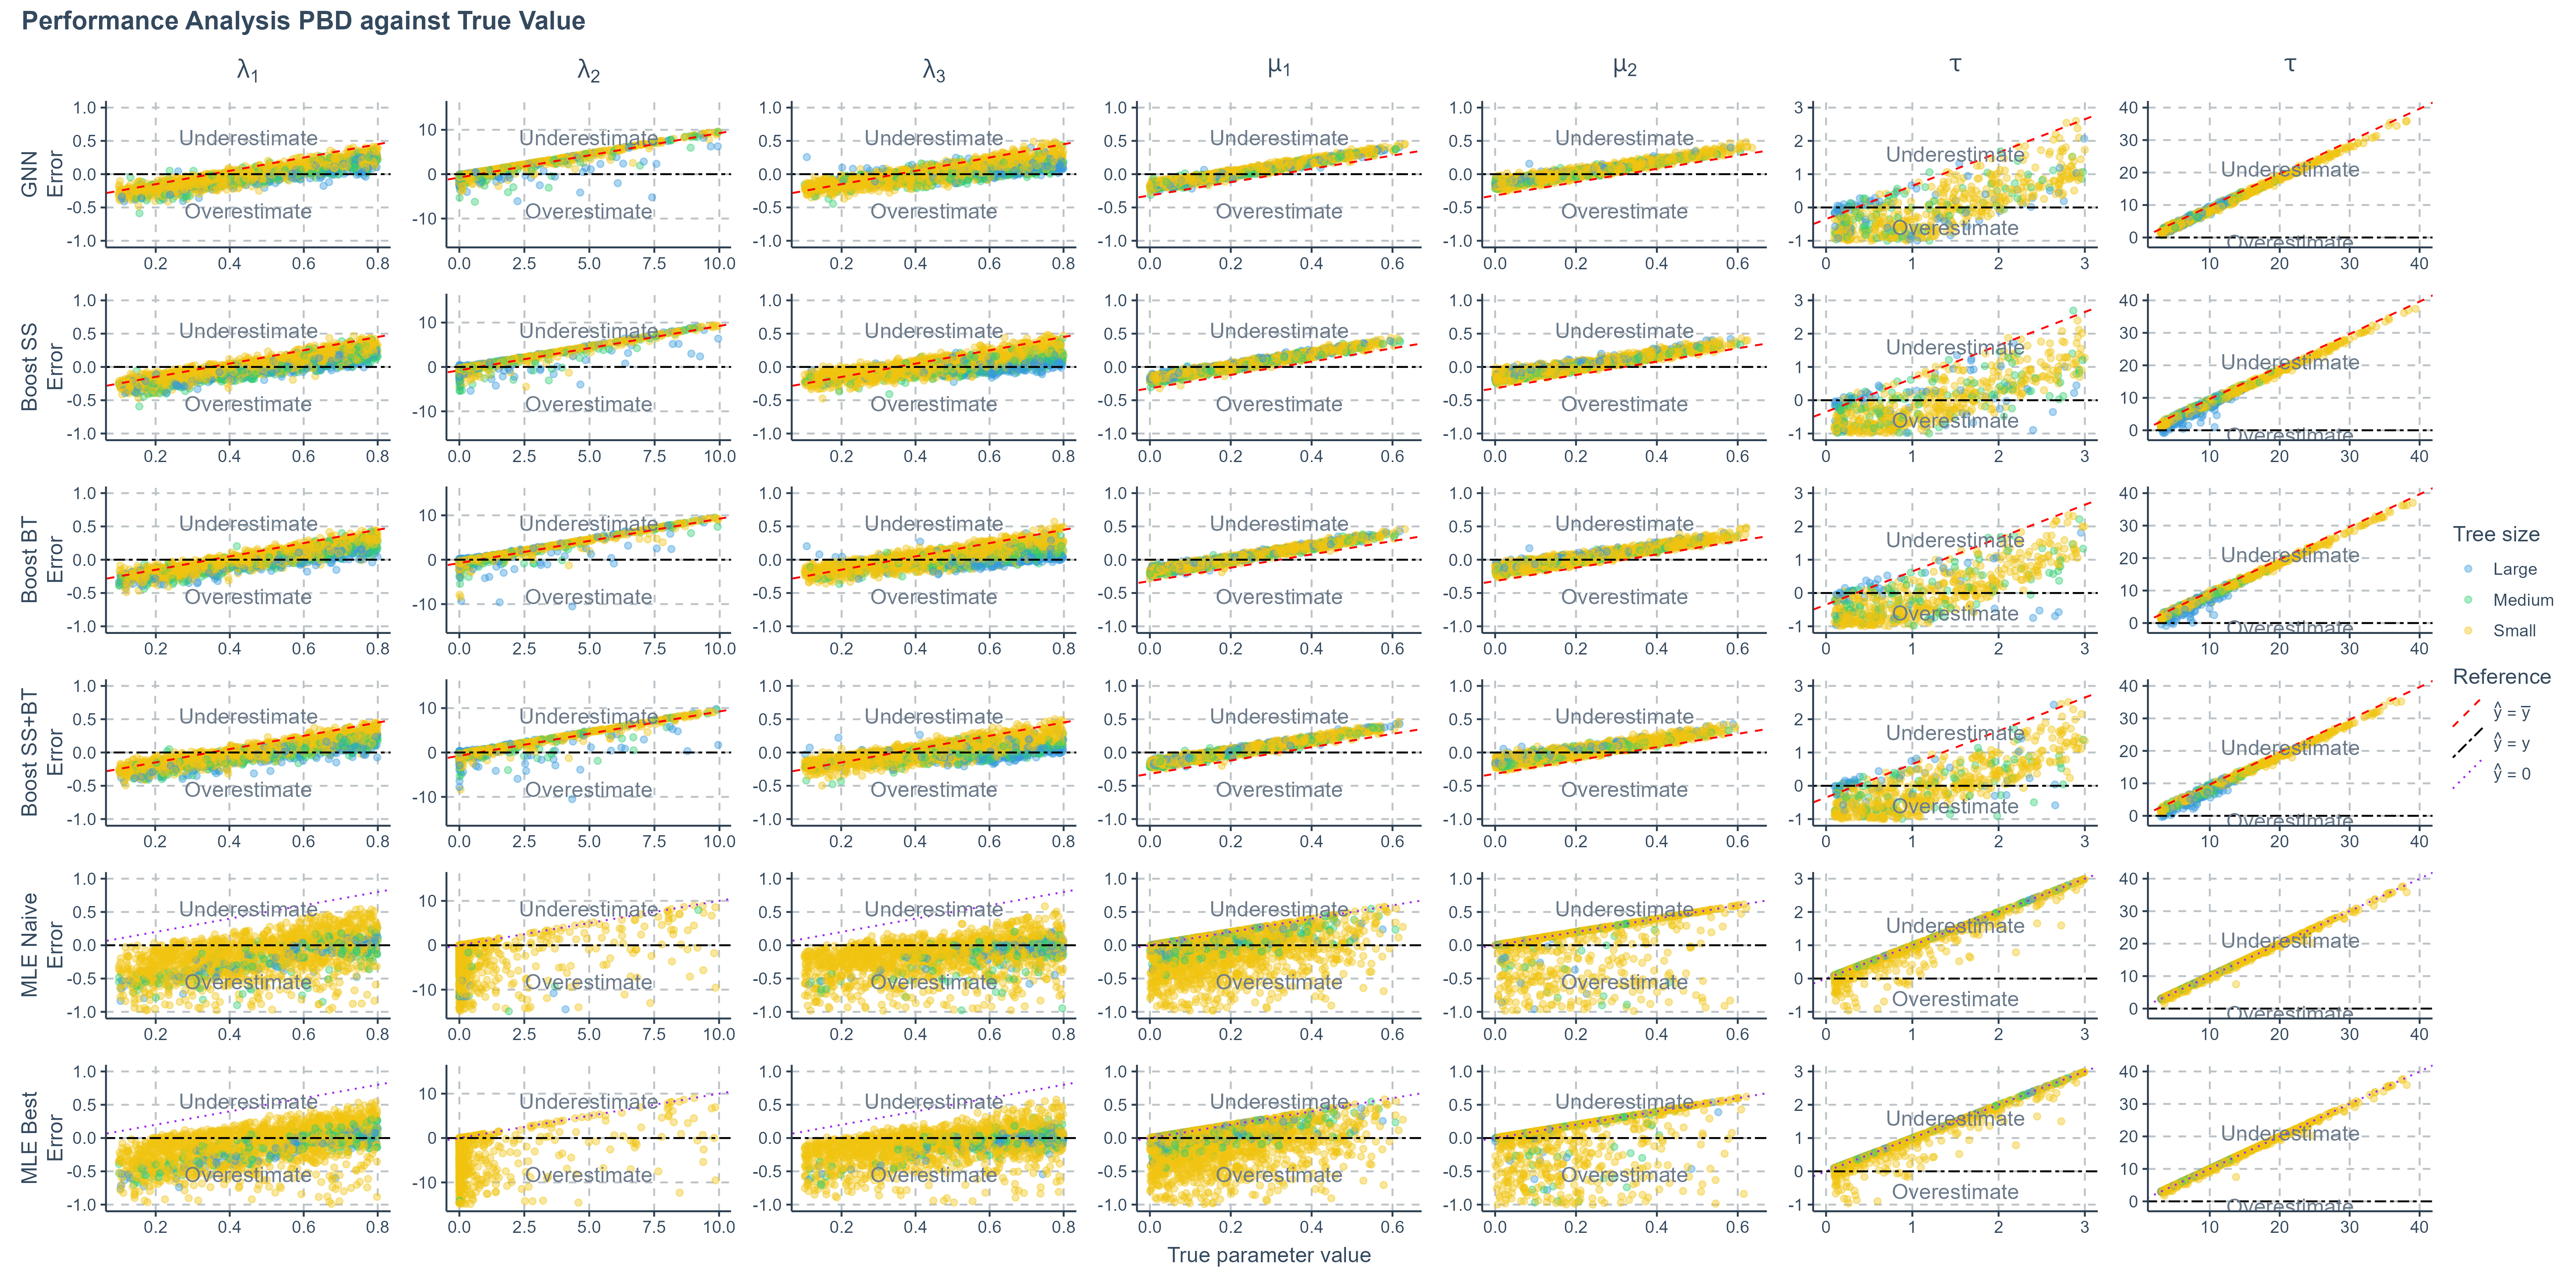
\includegraphics{chapter2/pbd_plot_true_value2.png}
    }
    \caption{The prediction error (absolute error) of various methods applied to phylogenies simulated under a protracted birth-death scenario, against true values. The errors shown are the differences between the true parameters used to simulate the phylogenies and the values predicted or estimated by each method. Each row represents a method, and each column corresponds to the results for one specific parameter. Phylogenies are categorized based on their size: yellow for small phylogenies with fewer than 200 nodes (including root, internal, and tip nodes), green for medium-sized phylogenies with 200 to 500 nodes, and blue for large phylogenies with more than 500 nodes. GNN: Predictions obtained by the graph neural network using the phylogenies. Boost SS: Boosting strategy that corrects GNN results using DNN. Boost BT: Boosting strategy that corrects GNN results using LSTM. Boost SS+BT: Sequential correction of GNN errors first using DNN, followed by LSTM. MLE Naive: Maximum Likelihood Estimation results using random starting points for parameter optimization. MLE Best: MLE results using the true parameter values as the starting points for optimization. Red dashed lines in panels representing neural network results indicate the mid-points of the parameter spaces. Purple dotted lines in MLE result panels signify where estimated values are 0. X-axis: True parameter values. Y-axis: Error, or difference between true and predicted values. $\lambda_1$: Speciation initiation rate of the good species. $\lambda_2$: Speciation completion rate. $\lambda_3$: Speciation initiation rate of the incipient species. $\mu_1$: Extinction rate of the good species. $\mu_2$: Extinction rate of the incipient species. $\tau$: Expected duration of speciation.}
    \label{fig::pbd_true_value}
\end{figure}

\begin{figure}[H]
    \centering
    \resizebox{1.0\textwidth}{!}{
        \includegraphics{chapter2/pbd_plot_tree_size2.png}
    }
    \caption{The prediction error (absolute error) of various methods applied to phylogenies simulated under a protracted birth-death scenario, against the total number of nodes in the phylogenies. The errors shown are the differences between the true parameters used to simulate the phylogenies and the values predicted or estimated by each method. Each row represents a method, and each column corresponds to the results for one specific parameter. Phylogenies are categorized based on their size into three sectors within each panel, separated by four vertical red dashed lines. From left to right, the sectors are: small phylogenies with fewer than 200 nodes (including root, internal, and tip nodes), medium-sized phylogenies with 200 to 500 nodes, and large phylogenies with more than 500 nodes. Color Coding: The color of the data points illustrates the expected duration of speciation. The color gradient transitions from light purple to dark blue, indicating increasing value of the duration. This scale is transformed using square root for clearer visual differentiation. GNN: Predictions obtained by the graph neural network using the phylogenies. Boost SS: Boosting strategy that corrects GNN results using DNN. Boost BT: Boosting strategy that corrects GNN results using LSTM. Boost SS+BT: Sequential correction of GNN errors first using DNN, followed by LSTM. MLE Naive: Maximum Likelihood Estimation results using random starting points for parameter optimization. MLE Best: MLE results using the true parameter values as the starting points for optimization. X-axis: Size of the phylogenies. Y-axis: Error. $\lambda_1$: Speciation initiation rate of the good species. $\lambda_2$: Speciation completion rate. $\lambda_3$: Speciation initiation rate of the incipient species. $\mu_1$: Extinction rate of the good species. $\mu_2$: Extinction rate of the incipient species. $\tau$: Expected duration of speciation.}
    \label{fig::pbd_tree_size}
\end{figure}

\begin{figure}[H]
    \centering
    \resizebox{1.0\textwidth}{!}{
        \includegraphics{chapter2/pbd_plot_durspec2.png}
    }
    \caption{The prediction error (absolute error) of various methods applied to phylogenies simulated under a protracted birth-death scenario, against the true mean duration of speciation. The errors shown are the differences between the true parameters used to simulate the phylogenies and the values predicted or estimated by each method. Each row represents a method, and each column corresponds to the results for one specific parameter. Color Coding: The color of the data points illustrates the total number of nodes of the phylogenies. The color gradient transitions from light purple to dark blue, indicating increasing value of the node number. This scale is transformed using square root for clearer visual differentiation. GNN: Predictions obtained by the graph neural network using the phylogenies. Boost SS: Boosting strategy that corrects GNN results using DNN. Boost BT: Boosting strategy that corrects GNN results using LSTM. Boost SS+BT: Sequential correction of GNN errors first using DNN, followed by LSTM. MLE Naive: Maximum Likelihood Estimation results using random starting points for parameter optimization. MLE Best: MLE results using the true parameter values as the starting points for optimization. X-axis: Size of the phylogenies. Y-axis: Error. $\lambda_1$: Speciation initiation rate of the good species. $\lambda_2$: Speciation completion rate. $\lambda_3$: Speciation initiation rate of the incipient species. $\mu_1$: Extinction rate of the good species. $\mu_2$: Extinction rate of the incipient species. $\tau$: Expected duration of speciation.}
    \label{fig::pbd_durspec}
\end{figure}

\begin{figure}[H]
    \centering
    \resizebox{0.85\textwidth}{!}{
        \includegraphics{chapter2/pbd_durspec_pars.png}
    }
    \caption{The correlation between the mean duration of speciation and the true parameter values under the protracted birth-death diversification scenario. Phylogenies are categorized based on their size: yellow for small phylogenies with fewer than 200 nodes (including root, internal, and tip nodes), green for medium-sized phylogenies with 200 to 500 nodes, and blue for large phylogenies with more than 500 nodes. X-axis: Mean duration of speciation. Y-axis: Tree size.}
    \label{fig::pbd_corr_durspec_pars}
\end{figure}

\clearpage
\subsection{Comparison between Our Methods and Existing Methods}
\label{appendix::established}
To benchmark our approaches against a convolutional architecture, we replaced the “Median” bagging panel in all performance figures related to the DDD scenario with a “CNN1D” panel reflecting the implementation of \citet{voznica_deep_2022}. This allows a direct side‐by‐side comparison between our neural networks and one of the best‐performing 1D‐CNNs in the literature.

Overall, the architecture by \citet{voznica_deep_2022} performed similarly and exhibited similar patterns as our approaches. CNN1D better recovered the carrying capacity effect strength than than GNN, DNN and LSTM alone, but lagged behind our boosting approaches--except for Boost BT+SS--in overall parameter prediction accuracy.

See the figures below for details.

\begin{figure}[H]
    \centering
    \resizebox{1.0\textwidth}{!}{
        \includegraphics{chapter2/ddd_plot_true_value_lambda_cnn1d2.png}
    }
    \caption{Prediction error of speciation rate plotted against true speciation rate under a diversity-dependent diversification scenario. Compared to the original figure in the results section, the "Median" bagging approach panel is replaced with "CNN1D" established by \citet{voznica_deep_2022}.}
    \label{fig::ddd_lambda_cnn1d}
\end{figure}

\begin{figure}[H]
    \centering
    \resizebox{1.0\textwidth}{!}{
        \includegraphics{chapter2/ddd_plot_true_value_mu_cnn1d2.png}
    }
    \caption{Prediction error of extinction rate plotted against true extinction rate under a diversity-dependent diversification scenario. Compared to the original figure in the results section, the "Median" bagging approach panel is replaced with "CNN1D" established by \citet{voznica_deep_2022}.}
    \label{fig::ddd_mu_cnn1d}
\end{figure}

\begin{figure}[H]
    \centering
    \resizebox{1.0\textwidth}{!}{
        \includegraphics{chapter2/ddd_plot_true_value_cap_cnn1d2.png}
    }
    \caption{Prediction error of carrying capacity plotted against true carrying capacity under a diversity-dependent diversification scenario. Compared to the original figure in the results section, the "Median" bagging approach panel is replaced with "CNN1D" established by \citet{voznica_deep_2022}.}
    \label{fig::ddd_cap_cnn1d}
\end{figure}

\begin{figure}[H]
    \centering
    \resizebox{1.0\textwidth}{!}{
        \includegraphics{chapter2/ddd_plot_true_value_cap_effect_cnn1d2.png}
    }
    \caption{Prediction error of effect strength of carrying capacity plotted against true effect strength of carrying capacity under a diversity-dependent diversification scenario. Compared to the original figure in the results section, the "Median" bagging approach panel is replaced with "CNN1D" established by \citet{voznica_deep_2022}.}
    \label{fig::ddd_cap_effect_cnn1d}
\end{figure}

\clearpage
\begin{figure}[H]
    \centering
    \resizebox{1.0\textwidth}{!}{
        \includegraphics{chapter2/ddd_plot_treesize_cnn1d2.png}
    }
    \caption{Prediction error of estimated parameters on trees of different sizes under a diversity-dependent diversification scenario. Compared to the original figure in the results section, the "Median" bagging approach panel is replaced with "CNN1D" established by \citet{voznica_deep_2022}.}
    \label{fig::ddd_tree_size_cnn1d}
\end{figure}

\clearpage
\subsection{Dataset Re-balancing}
\label{appendix::rebalance}
Birth-death processes without carrying capacity effect may have larger variance of tree size than the DDD trees. A skew in the frequency of tree size across datasets may appear that leads to a non-representative sample. 

To address this issue, we re-balanced the BD dataset by creating 10 bins, each designated to hold phylogenies within specific size ranges, spanning from 10 to 2000 nodes in increments of 200 nodes per bin (the first bin accepts phylogeny of sizes 10 to 200). We randomly simulated phylogenies using parameters sampled from the same space as the BD training dataset and allocated them to these bins according to their sizes, continuing this process until each bin reached its target capacity of 10,000 phylogenies. This method leads to a more equal representation of phylogenies of each size range, reducing size-based sampling bias. The filled bins were subsequently combined to form a re-balanced dataset, which in total has 100,000 phylogenies.

To compare with the original BD dataset, we trained neural networks on the re-balanced dataset, and validated neural network performance on an additional testing dataset (10,000 phylogenies simulated using the same parameter space). We computed MLE estimates on 2,000 randomly sampled phylogenies from the testing dataset. See \autoref{fig::bd_rebalance} for the results.

\emph{(Figure on next page.)}

\clearpage
\begin{figure}[H]
    \centering
    \resizebox{0.8\textwidth}{!}{
        \includegraphics{chapter2/bd_plot_tree_rebalance.png}
    }
    \caption{The prediction error (absolute error) of various methods applied to re-balanced phylogenies simulated under a birth-death scenario, against the total number of nodes in the phylogenies. The errors shown are the differences between the true parameters used to simulate the phylogenies and the values predicted or estimated by each method. Each row represents a method, and each column corresponds to the results for one specific parameter. Phylogenies are categorized based on their size into three sectors within each panel, separated by four vertical red dashed lines. From left to right, the sectors are: small phylogenies with fewer than 200 nodes (including root, internal, and tip nodes), medium-sized phylogenies with 200 to 500 nodes, and large phylogenies with more than 500 nodes. This scale is transformed using square root for clearer visual differentiation. GNN: Predictions obtained by the graph neural network using the phylogenies. Boost SS: Boosting strategy that corrects GNN results using DNN. Boost BT: Boosting strategy that corrects GNN results using LSTM. Boost SS+BT: Sequential correction of GNN errors first using DNN, followed by LSTM. MLE Naive: Maximum Likelihood Estimation results using random starting points for parameter optimization. MLE Best: MLE results using the true parameter values as the starting points for optimization. X-axis: Size of the phylogenies. Y-axis: Error. $\lambda$: Speciation rate. $\mu$: Extinction rate.}
    \label{fig::bd_rebalance}
\end{figure}

\clearpage
\subsection{Data outside the Training Space and Complete Phylogeny}
\label{appendix::generalization_full_tree}
We simulated additional datasets to explore the generalization ability of the neural networks when facing data with true parameters completely outside the training space, as well as to compare neural network performances between extant and complete phylogenies. Each simulated dataset was divided into in-distribution and out-of-distribution datasets. We used the in-distribution datasets for training and testing and the out-of-distribution datasets for evaluating the generalization ability of the trained neural networks. Validating trained neural networks on the out-of-distribution datasets can provide insights into whether their performances are tailored to the peculiarities of the already seen data and whether they are robust to new, unseen phylogenies. For each tree we kept two versions: tree of all species (TAS) and tree of extant species (TES). See \autoref{table::simulated_trees_in_out_sample} for the parameter settings of the additional datasets, see \autoref{table::simulation_in_out_sample} for the criteria of in-distribution and out-of-distribution dataset separation. To conserve GPU memory, the parameter space for additional datasets was deliberately kept smaller, given that the TAS dataset inherently contains far more information than the TES.

\begin{figure}[ht]
    \centering
    \resizebox{1.0\textwidth}{!}{
        \includegraphics{chapter2/differences_box.png}
    }
    \caption{Comparisons of relative differences (in percentage) between ground true and estimated parameter values. From top to bottom, the panels in each row present the relative differences of trees generated by a specific diversification process. From left to right, the panels in each column present the relative differences of a specific parameter used when simulating the trees. Within each panel, each box represents a specific method for parameter estimation on a specific data set (as described in x-axis labels). Red boxes represent parameter estimation by using only graph neural network (GNN) on the in-sample datasets (Test in figure), yellow boxes represent the non-optimal maximum likelihood estimation (MLE) method on the complete datasets (direct outputs from simulation, without any separation), green boxes represent the optimal MLE method on the complete datasets, purple boxes represent parameter estimation by GNN on the out-of-sample datasets. BD - birth-death trees; DDD - diversity-dependent-diversification trees; PBD - protracted birth-death trees. $\lambda$ - birth rate/intrinsic speciation rate; $\mu$ death rate/intrinsic extinction rate; $K$ - carrying capacity; $\lambda_1$ - speciation rate of good species; $\lambda_2$ - speciation-completion rate; $\lambda_3$ - speciation rate of incipient species; $\mu_1$ - extinction rate of good species; $\mu_2$ extinction rate of incipient species. T-TAS - GNN parameter estimation on full trees (with extinct lineages) in the in-sample data set; T-TES - GNN parameter estimation on extant trees (without extinct lineages) in the in-sample dataset; MLE-TES - MLE parameter estimation on extant trees in the complete dataset; V-TAS - GNN parameter estimation on full trees in the out-of-sample dataset; V-TES - GNN parameter estimation on extant trees in the out-of-sample dataset.}
    \label{fig::differences_box}
\end{figure}

\begin{table}[ht]
    \caption{List of simulated tree datasets. The type column specifies which function is used to generate the trees. The age column specifies the crown age of the trees. The N column specifies the number of trees in the dataset. The rest of the columns specify the lower ($a$) and the upper ($b$) bounds of the initial parameters for the tree simulations, all the parameters are sampled from $U(a, b)$ except for $\lambda_1$ of the protracted birth-death scenario. $\lambda_1$ is computed as $\lambda_1 = 10^e$ where $e$ is sampled from $U(-3, 1)$. $U$ denotes uniform distribution. List A shows the parameter distributions of the birth-death trees and the diversity-dependent-diversification trees, $\lambda$: intrinsic speciation rate/birth rate; $\mu$: intrinsic extinction rate/death rate; $K$: carrying capacity. List B shows the parameter distributions of the protracted birth-death trees, $\lambda_1$: speciation-initiation rate of good species; $\lambda_2$: speciation-completion rate; $\lambda_3$: speciation-initiation rate of incipient species; $\mu_1$: extinction rate of good species; $\mu_2$: extinction rate of incipient species. $^*$In diversity-dependent-diversification simulations, the maximum extinction rate is capped at 1.5 if $0.9\lambda > 1.5$.}
    \noindent
\begin{tabular}{@{}lllllllll@{}}
\multicolumn{9}{l}{\textbf{A:} Parameter settings for BD and DDD trees} \\ \toprule
\multicolumn{1}{c}{\multirow{2}{*}{\textbf{Type}}} & \multicolumn{1}{c}{\multirow{2}{*}{\textbf{Age}}} & \multicolumn{1}{c}{\multirow{2}{*}{\textbf{N}}} & \multicolumn{2}{c}{\textbf{$\lambda_0$}}                   & \multicolumn{2}{c}{\textbf{$\mu_0$}}                   & \multicolumn{2}{c}{$K$}                             \\ \cmidrule(l){4-5} \cmidrule(l){6-7} \cmidrule(l){8-9}  
\multicolumn{1}{c}{}                                & \multicolumn{1}{c}{}                              & \multicolumn{1}{c}{}                               & \multicolumn{1}{c}{$a$} & \multicolumn{1}{c}{$b$} & \multicolumn{1}{c}{$a$} & \multicolumn{1}{c}{$b$} & \multicolumn{1}{c}{$a$} & \multicolumn{1}{c}{$b$} \\ \midrule
BD                                                  & 10                                                & 60k                                             & 0.1                     & 0.6                     & 0.0                     & 0.9$\lambda_0$                     & -                       & -                       \\
DDD                                                 & 10                                                & 100k                                             & 0.1                     & 3.0                     & 0.0                     & ${0.9\lambda_0}^*$                     & 10                 & 1000                 \\\bottomrule
\end{tabular}
\newline
\vspace{0.2 cm}
\newline
\begin{tabular}{@{}lllllllllllll@{}}
\multicolumn{13}{l}{\textbf{B:} Parameter settings for PBD trees} \\ \toprule
\multicolumn{1}{c}{\multirow{2}{*}{\textbf{Type}}} & \multicolumn{1}{c}{\multirow{2}{*}{\textbf{Age}}} & \multicolumn{1}{c}{\multirow{2}{*}{\textbf{N}}} & \multicolumn{2}{c}{\textbf{$b_1$}}                  & \multicolumn{2}{c}{\textbf{$\lambda_1$}}                  & \multicolumn{2}{c}{\textbf{$b_2$}}                  & \multicolumn{2}{c}{\textbf{$\mu_1$}}                  & \multicolumn{2}{c}{\textbf{$\mu_2$}}                  \\ \cmidrule(l){4-5} \cmidrule(l){6-7} \cmidrule(l){8-9} \cmidrule(l){10-11} \cmidrule(l){12-13} 
\multicolumn{1}{c}{}                                & \multicolumn{1}{c}{}                                & \multicolumn{1}{c}{}                              & \multicolumn{1}{c}{$a$} & \multicolumn{1}{c}{$b$} & \multicolumn{1}{c}{$a$} & \multicolumn{1}{c}{$b$} & \multicolumn{1}{c}{$a$} & \multicolumn{1}{c}{$b$} & \multicolumn{1}{c}{$a$} & \multicolumn{1}{c}{$b$} & \multicolumn{1}{c}{$a$} & \multicolumn{1}{c}{$b$} \\ \midrule
PBD                                                 & 10                                                & 100k                                              & 0.1                     & 0.8                     & 0.001                     & 10                     & 0.1                     & 0.8                     & 0.0                     & 0.8$b_1$                     & 0.0                     & 0.8$b_2$                     \\ \bottomrule
\end{tabular}
    \label{table::simulated_trees_in_out_sample}
\end{table}

\begin{table}[ht]
    \caption{Criteria for in-distribution (in-sample) and out-of-distribution (out-of-sample) dataset separation. Trees generated from each model are separated into left out-of-sample group, in-sample group and right out-of-sample group, based on the parameter ranges. The Model column shows the model of a parameter; the Parameter column shows the corresponding parameter; the Left Out column shows the criteria for the left out-of-sample group; the In Sample column shows the criteria for the in-sample group; the Right Out column shows the criteria of the right out-of-sample group. $\lambda$: intrinsic speciation rate/birth rate; $\mu$: intrinsic extinction rate/death rate; $K$: carrying capacity. List B shows the parameter distributions of the protracted birth-death trees, $\lambda_1$: speciation-initiation rate of good species; $\lambda_2$: speciation-completion rate; $\lambda_3$: speciation-initiation rate of incipient species; $\mu_1$: extinction rate of good species; $\mu_2$: extinction rate of incipient species.}
    \begin{tabular}{@{}lllll@{}}
\toprule
Model & Parameter   & Left Out         & In      & Right Out      \\ \midrule
BD    & $\lambda_0$ & $[0.10, 0.18)$   & $[0.18, 0.52]$ & $(0.52, 0.60]$ \\
BD    & $\mu_0$     & $[0.00, 0.08)$   & $[0.08, 0.46]$ & $(0.46, 0.54]$ \\
DDD   & $\lambda_0$ & $[0.00, 0.30)$   & $[0.30, 2.70]$ & $(2.70, 3.00]$ \\
DDD   & $\mu_0$     & $[0.00, 0.10)$   & $[0.10, 0.80]$ & $(0.80, 0.90]$ \\
DDD   & $K$         & $[10, 100)$      & $[100, 900]$   & $(900, 1000]$  \\
PBD   & $b_1$       & $[0.10, 0.18)$   & $[0.18, 0.72]$ & $(0.72, 0.80]$ \\
PBD   & $\lambda_1$ & $[0.001, 0.002)$ & $[0.002, 5]$   & $(5, 10]$      \\
PBD   & $b_2$       & $[0.10, 0.18)$   & $[0.18, 0.72]$ & $(0.72, 0.80]$ \\
PBD   & $\mu_1$      & $[0.00, 0.06)$   & $[0.06, 0.58]$ & $(0.58, 0.64]$ \\
PBD   & $\mu_2$      & $[0.00, 0.06)$   & $[0.06, 0.58]$ & $(0.58, 0.64]$ \\ \bottomrule
\end{tabular}
    \label{table::simulation_in_out_sample}
\end{table}

\clearpage
\subsection{Learning from Summary Statistics}
\label{appendix::learn_from_stats}
To analyze the relationships between summary statistics and the true parameters used in the diversity-dependent diversification simulations, we computed Pearson correlation indices for each summary statistic against the true values of the three parameters. The absolute values of the correlations are visualized as a heatmap, detailed in \autoref{fig::ddd_corr_stats}.

\begin{figure}[H]
    \centering
    \resizebox{1.0\textwidth}{!}{
        \includegraphics{chapter2/ddd_corr_stats.png}
    }
    \caption{Heatmap of absolute correlation strengths between true parameters and summary statistics from simulated trees under a diversity-dependent diversification scenario. Each column corresponds to a specific summary statistic, while each row corresponds to a true parameter that was used to simulate the phylogenies. The true parameters are denoted as follows: $\lambda$ for speciation rate, $\mu$ for extinction rate, and $K$ for carrying capacity. The color gradient, ranging from dark purple to yellow, represents the increasing values of the absolute Pearson correlations between the summary statistics and the true parameters, See \autoref{appendix::list_stats} for the details of the statistics.}
    \label{fig::ddd_corr_stats}
\end{figure}

The heatmap analysis reveals that a large number of summary statistics showed a high correlation with carrying capacity, whereas strong correlations with speciation and extinction rates are considerably less frequent. Generally, the correlation strength between the true parameters and extinction rate is markedly lower. These findings align with the observed performance of DNN, which generally yields good estimates for carrying capacity but is much less effective in accurately predicting speciation rates and particularly poor at estimating extinction rates. 

We further evaluated the DNN's performance by benchmarking it against a range of non-neural-network regression techniques using the same summary statistics. These included multivariate linear regression, Ridge regression, Lasso regression, random forest regression, and gradient boosting regression. Our findings indicated that while these traditional regression and machine learning methods generally outperformed the DNN, they still did not match the performance of our more complex neural networks.

Traditional regression methods and other machine learning techniques often outperform linear feed-forward neural networks in classical regression tasks. Such methods can stabilize performance with less data compared to neural networks, which usually require large datasets to generalize effectively. In our study, the dataset size -- consisting of 100,000 entries across 54 statistics -- may seem substantial, but it is still relatively modest when tasked with regressing multiple parameters simultaneously.

Despite these findings, DNNs have shown efficacy in enhancing the performance of other neural networks, particularly through the prediction of residuals using summary statistics. DNN might not be the optimal choice for estimating parameters from summary statistics alone, but they can be valuable in ensemble learning strategies.

\clearpage
\subsection{Meta Information of the Selected Empirical Trees}
\label{appendix::meta_info_empirical_trees}
\begin{longtable}{@{}lll@{}} 
\toprule
Family      & Tree                & Ntip \\ \midrule
Amphibia    & Caecilidae          & 31   \\
Amphibia    & Hynobiidae          & 46   \\
Amphibia    & Salamandridae       & 42   \\
Amphibia    & Plethodontidae      & 278  \\
Amphibia    & Pipidae             & 23   \\
Amphibia    & Eleutherodactylidae & 145  \\
Amphibia    & Ranidae             & 218  \\
Bird        & Tyrannidae          & 419  \\
Bird        & Thraupidae          & 370  \\
Bird        & Psittacidae         & 330  \\
Bird        & Trochilidae         & 334  \\
Bird        & Columbidae          & 306  \\
Bird        & Furnariidae         & 302  \\
Bird        & Muscicapidae        & 279  \\
Bird        & Accipitridae        & 242  \\
Bird        & Picidae             & 223  \\
Bird        & Thamnophilidae      & 219  \\
Bird        & Fringillidae        & 194  \\
Bird        & Strigidae           & 191  \\
Bird        & Turdidae            & 170  \\
Bird        & Meliphagidae        & 177  \\
Bird        & Phasianidae         & 176  \\
Bird        & Emberizidae         & 163  \\
Bird        & Anatidae            & 157  \\
Bird        & Cisticolidae        & 142  \\
Bird        & Pycnonotidae        & 124  \\
Bird        & Rallidae            & 125  \\
Bird        & Cuculidae           & 138  \\
Bird        & Estrildidae         & 140  \\
Bird        & Nectariniidae       & 127  \\
Bird        & Leiothrichidae      & 127  \\
Bird        & Corvidae            & 120  \\
Bird        & Zosteropidae        & 120  \\
Bird        & Sturnidae           & 109  \\
Bird        & Parulidae           & 109  \\
Bird        & Ploceidae           & 108  \\
Bird        & Icteridae           & 102  \\
Bird        & Apodidae            & 99   \\
Bird        & Laridae             & 99   \\
Bird        & Alaudidae           & 91   \\
Bird        & Monarchidae         & 87   \\
Bird        & Scolopacidae        & 89   \\
Bird        & Caprimulgidae       & 88   \\
Bird        & Alcedinidae         & 91   \\
Bird        & Campephagidae       & 80   \\
Bird        & Procellariidae      & 81   \\
Bird        & Hirundinidae        & 83   \\
Bird        & Troglodytidae       & 79   \\
Bird        & Phylloscopidae      & 71   \\
Bird        & Ardeidae            & 61   \\
Bird        & Pellorneidae        & 66   \\
Bird        & Sylviidae           & 62   \\
Bird        & Cardinalidae        & 68   \\
Bird        & Charadriidae        & 64   \\
Bird        & Falconidae          & 64   \\
Bird        & Motacillidae        & 62   \\
Bird        & Acanthizidae        & 63   \\
Bird        & Cotingidae          & 65   \\
Bird        & Vireonidae          & 58   \\
Bird        & Acrocephalidae      & 52   \\
Bird        & Bucerotidae         & 55   \\
Bird        & Paridae             & 53   \\
Bird        & Pachycephalidae     & 50   \\
Bird        & Locustellidae       & 53   \\
Bird        & Rhinocryptidae      & 53   \\
Bird        & Timaliidae          & 55   \\
Bird        & Cracidae            & 50   \\
Bird        & Pipridae            & 52   \\
Bird        & Grallariidae        & 49   \\
Bird        & Malaconotidae       & 46   \\
Bird        & Passeridae          & 48   \\
Bird        & Rhipiduridae        & 42   \\
Bird        & Dicaeidae           & 45   \\
Bird        & Tinamidae           & 47   \\
Bird        & Petroicidae         & 44   \\
Bird        & Ramphastidae        & 35   \\
Bird        & Tityridae           & 41   \\
Bird        & Trogonidae          & 42   \\
Bird        & Lybiidae            & 41   \\
Bird        & Paradisaeidae       & 40   \\
Bird        & Phalacrocoracidae   & 33   \\
Bird        & Bucconidae          & 35   \\
Bird        & Threskiornithidae   & 34   \\
Bird        & Mimidae             & 34   \\
Bird        & Odontophoridae      & 34   \\
Bird        & Oriolidae           & 30   \\
Bird        & Laniidae            & 29   \\
Bird        & Pittidae            & 31   \\
Bird        & Platysteiridae      & 30   \\
Bird        & Cettiidae           & 32   \\
Bird        & Megalaimidae        & 28   \\
Bird        & Maluridae           & 27   \\
Bird        & Sittidae            & 24   \\
Bird        & Meropidae           & 26   \\
Bird        & Dicruridae          & 24   \\
Bird        & Otididae            & 25   \\
Bird        & Alcidae             & 23   \\
Bird        & Hydrobatidae        & 22   \\
Bird        & Musophagidae        & 23   \\
Bird        & Megapodiidae        & 21   \\
Bird        & Cacatuidae          & 21   \\
Bird        & Diomedeidae         & 21   \\
Bird        & Vangidae            & 21   \\
CrocoTurtle & Crocodylia          & 25   \\
CrocoTurtle & Testudines          & 233  \\
Mammal      & Vespertilionidae    & 386  \\
Mammal      & Soricidae           & 329  \\
Mammal      & Sciuridae           & 276  \\
Mammal      & Pteropodidae        & 174  \\
Mammal      & Phyllostomidae      & 150  \\
Mammal      & Bovidae             & 138  \\
Mammal      & Cercopithecidae     & 127  \\
Mammal      & Molossidae          & 98   \\
Mammal      & Didelphidae         & 84   \\
Mammal      & Hipposideridae      & 74   \\
Mammal      & Rhinolophidae       & 73   \\
Mammal      & Echimyidae          & 69   \\
Mammal      & Dasyuridae          & 63   \\
Mammal      & Mustelidae          & 59   \\
Mammal      & Heteromyidae        & 58   \\
Mammal      & Leporidae           & 58   \\
Mammal      & Macropodidae        & 56   \\
Mammal      & Nesomyidae          & 55   \\
Mammal      & Ctenomyidae         & 51   \\
Mammal      & Dipodidae           & 51   \\
Mammal      & Emballonuridae      & 49   \\
Mammal      & Cebidae             & 48   \\
Mammal      & Cervidae            & 45   \\
Mammal      & Felidae             & 40   \\
Mammal      & Talpidae            & 39   \\
Mammal      & Geomyidae           & 38   \\
Mammal      & Pitheciidae         & 37   \\
Mammal      & Canidae             & 34   \\
Mammal      & Delphinidae         & 34   \\
Mammal      & Viverridae          & 34   \\
Mammal      & Herpestidae         & 33   \\
Mammal      & Spalacidae          & 31   \\
Mammal      & Ochotonidae         & 28   \\
Mammal      & Gliridae            & 27   \\
Mammal      & Tenrecidae          & 25   \\
Mammal      & Atelidae            & 24   \\
Mammal      & Erinaceidae         & 22   \\
Mammal      & Phalangeridae       & 22   \\
Squamate    & Xantusiidae         & 26   \\
Squamate    & Gerrhosauridae      & 28   \\
Squamate    & Cordylidae          & 42   \\
Squamate    & Varanidae           & 53   \\
Squamate    & Chamaeleonidae      & 142  \\
Squamate    & Iguanidae           & 31   \\
Squamate    & Phrynosomatidae     & 114  \\
Squamate    & Pythonidae          & 26   \\
Squamate    & Viperidae           & 209  \\ \bottomrule
\end{longtable}

\clearpage
\subsection{List of Summary Statistics}
\label{appendix::list_stats}
\begin{minipage}{\linewidth}
\centering
\setlength{\tabcolsep}{10pt}
\renewcommand{\arraystretch}{1.15}
\small

\begin{tabularx}{\linewidth}{@{}>{\raggedright\arraybackslash}X
                          >{\raggedright\arraybackslash}X@{}}
\toprule
\multicolumn{2}{c}{\textbf{Summary Statistics}}\\
\midrule
Gamma & Area Per Pair (aPP)\\
Sackin & Average Leaf Depth (aLD)\\
Colless & I Statistic\\
Aldous' Beta Statistic & ewColless\\
Blum & Max Delta Width (maxDelW)\\
Crown Age & Maximum of Depth\\
Tree Height & Variance of Depth\\
Pigot's Rho & Maximum Width\\
Number of Lineages & Rogers\\
nLTT with Empty Tree & Total Cophenetic Distance\\
Phylogenetic Diversity & Symmetry Nodes\\
AvgLadder Index & Mean Pairwise Distance (mpd)\\
Cherries & Variance Pairwise Distance (vpd)\\
ILnumber & Phylogenetic Species Variability (psv)\\
Pitchforks & Mean Nearest Taxon Distance (mntd)\\
Stairs & J Statistic of Entropy\\
Stairs2 & Rquartet Index\\
Laplacian Spectrum Asymmetry & Laplacian Spectrum Log Eigen\\
Laplacian Spectrum Peakedness & Laplacian Spectrum Eigengap\\
Number of Nodes & Wiener Index\\
B1 & Max Betweenness\\
B2 & Max Closeness\\
Diameter (no branch lengths) & Maximum Eigenvector Value\\
Mean Branch Length & Variance of Branch Length\\
Mean External Branch Length & Variance of External Branch Length\\
Mean Internal Branch Length & Variance of Internal Branch Length\\
Number of Imbalancing Steps & J\_One Statistic\\
\bottomrule
\end{tabularx}

\end{minipage}


\clearpage
\subsection{Computational Costs}
\label{appendix::compute_cost}
In our experiments, generating 100,000 phylogenies took 3--8 hours, depending on the scenario (BD, DDD, or PBD). MLE on BD models ran in about 2 hours for all 100,000 trees (with parallelization), whereas fitting DDD models could take up to 24 hours per tree and often failed. Neural-network costs split into training and inference: training on 100,000 trees for 100 epochs with boosting approaches can exceed 48 hours on high-end GPUs (e.g., NVIDIA A100), though simpler architectures (DNN, CNN1D and LSTM) finish in \approx2 hours. Once trained, even our most complex network predicts parameters for 100,000 trees in \approx45 minutes (including up to 30 minutes of data loading and preprocessing) under GPU acceleration.
}

%% Ch3
\chapter{Neural Recoverability under the \texttt{eve} Model}
\label{chapter3}
\blfootnote{{\color{rug-red} \faFile*[regular]}~Qin, T., van Benthem, K., Valente, L.\textsuperscript{\dag}, \& Etienne, R.\textsuperscript{\dag} Identifying evolutionary relatedness effects on diversification from phylogenies using neural networks. Manuscript in preparation. \textsuperscript{\dag} indicates joint senior authors.}

\dropcap{R}econstructing the forces that shaped macroevolutionary histories from extant phylogenies is fundamentally challenging: richly parameterized diversification models are often only weakly identifiable; different evolutionary mechanisms can yield nearly indistinguishable tree shapes. Here we use a model with evolutionary relatedness dependence to evaluate how much information about such forces can be recovered from simulated trees. We train graph neural networks and long short–term memory classifiers to distinguish three scenarios of feedback of diversity on diversification: effect of phylogenetic diversity (total branch length), evolutionary distinctiveness (average phylogenetic distance of a species to all other species in a clade), and nearest–neighbor distance (phylogenetic distance to the mostly closely related species). We also train a suite of regression networks to estimate the underlying diversification parameters. We then analyze classification performance, calibration of predicted class probabilities, regression errors, and their dependence on tree size and on the strength and sign of richness and relatedness effects. Across network architectures and complexity levels, scenario classification is only moderately accurate and strongly asymmetric as revealed by the confusion matrix. Trees generated under an effect of nearest–neighbor distance on diversification tend to be correctly classified, whereas those with an effect of evolutionary distinctiveness are frequently misclassified. Regression networks systematically shrink predictions toward the empirical mean, especially for complex models, suggesting broad regions of parameter space with low identifiability. Strong global dependence of diversification rates on diversity further erodes recoverability by driving large variations in tree size that mask the subtler signatures of relatedness effects. In contrast, sufficiently strong speciation-relatedness effects can carve out narrow regions of parameter space in which scenarios and parameters become practically recoverable. Together, our results provide a map of when neural networks can and cannot infer diversification mechanisms from extant trees under our evolutionary relatedness dependence model, and they underscore the need for additional data or constraints when using flexible diversification models for macroevolutionary inference.

\clearpage
{ % Constrain counter reset
% Hacky command for displaying Appendix citations
\renewcommand{\subsectionautorefname}{Appendix}
\section{Introduction}
\dropcap{T}ime‐calibrated phylogenies are now central tools for studying macroevolutionary dynamics. From such trees, we seek to reconstruct how speciation and extinction rates varied through time and across lineages, and how ecological limits and biotic interactions have shaped present-day diversity \citep{nee_tempo_1992, quental_diversity_2010}. Early work typically assumed constant diversification rates, which implies exponential lineage accumulation \citep{nee_extinction_1994, kubo_inferring_1995}. However, reconstructed phylogenies for many clades show pronounced slowdowns in lineages-through-time curves, inconsistent with simple constant-rate models and motivating a broad family of more flexible diversification models, including time-dependent, diversity-dependent, and protracted speciation models \citep{phillimore_density-dependent_2008, moen_why_2014, etienne_diversity-dependence_2012, etienne_prolonging_2012, rosindell_protracted_2010}. A common mechanistic theme in these models is that speciation rates decline as clades fill ecological or niche space, with species richness acting as a proxy for ecological limits \citep{srivastava_phylogenetic_2012, kondratyeva_reconciling_2019}. 

At the same time, there is growing recognition that extant phylogenies carry only limited information about past diversification histories. \citet{nee_reconstructed_1994} already showed that a constant-rate birth-death model is equivalent to a pure birth model with temporally declining speciation rate. This property allowed them to compute the probability of a phylogeny given the constant-rate birth-death model, but also implies that there is inherent indistinguishability of these models based on phylogenetic information alone. This result was generalized by \citet{louca_extant_2020}, who showed that, under general birth-death processes, an infinite number of distinct speciation-extinction trajectories can produce exactly the same distribution of extant time trees, forming large “congruence classes” of observationally equivalent models. Even for more constrained model families, branching patterns alone often cannot discriminate between alternative mechanisms. For instance, \citet{pannetier_branching_2021} demonstrated that diversity-dependent and purely time-dependent diversification models that share the same expected diversity‐through‐time curve are essentially indistinguishable from extant trees using standard likelihood methods. These results highlight that increasing model flexibility does not automatically yield more informative inferences.

The recently-developed \texttt{eve} model of \citet{qin_impact_2025} augments diversity-dependent diversification by allowing speciation and extinction rates to depend linearly on both species richness and a measure of evolutionary relatedness (ER) for each lineage. The rationale for this is that ER may have an effect in diversification rates that is independent from species diversity, for instance, if closely related species are more likely to compete for niches. ER can be defined at different phylogenetic scales, for example using clade-wide phylogenetic diversity (PD, total branch length in the tree) or more localized, lineage-specific metrics such as evolutionary distinctiveness (ED, average phylogenetic distance to all other species in the clade) or nearest-neighbor distance (NND, phylogenetic distance to the most closely related species). Depending on the signs and magnitudes of the richness and ER effects, \texttt{eve} can generate a wide range of branching patterns and tree shapes, and previous work has suggested that the PD, ED and NND variants can produce near identical tree-shape signatures for moderate effect sizes, in terms of classic phylogenetic summary statistics. 

The complexity and state dependence of \texttt{eve} make likelihood-based inference of parameters of the model analytically intractable, encouraging a shift toward simulation-based approaches. Neural networks and other deep-learning methods have recently been proposed to estimate diversification parameters and classify models from phylogenetic trees \citep{lajaaiti_comparison_2023, voznica_deep_2022, lambert_deep_2023, qin_parameter_2025}. These methods can learn from graph representations of trees, branching times and summary statistics, and for relatively simple birth-death or diversity-dependent models they can achieve performance comparable to, or potentially exceeding, maximum likelihood estimation. However, when applied to models already known to suffer from non-identifiability, such as protracted speciation \citep{etienne_estimating_2014}, neural networks tend to converge to conservative predictions that reflect the empirical mean of the training distribution rather than the true parameters. In such cases, the limiting factor appears to be the information content of the trees, even after extensive sweeps over neural network architectures, depths, and hyperparameter settings, rather than the expressive power of the estimator \citep{qin_parameter_2025}. This suggests that models as flexible as diversity-dependent diversification or protracted speciation may already lie close to the practical limits of what can be identified from extant trees, regardless of whether one uses maximum likelihood or neural networks, and thus there is little reason to expect neural networks to reliably recover all parameters of an even more complex model such as \texttt{eve}.

In this study we use neural networks as means to explore the putative limits of information content of phylogenies regarding diversification processes in complex models. We simulate large collections of extant trees under the three ER scenarios (PD, ED, NND), three levels of model complexity (2, 4 or 6 free parameters), and a broad range of effect sizes for the effects of species richness and evolutionary relatedness. We then train graph neural networks (GNNs) and long short-term memory (LSTM) networks as classifiers to distinguish PD, ED and NND, and as regressors (in an ensemble GNN+LSTM architecture as developed by \citet{qin_parameter_2025}) to recover the underlying parameters from tree representations and branching times. Performance is evaluated as a function of tree size, true parameter values, model complexity and regressor/classifier misspecification, using simulated tree datasets. 

By asking when these neural network learners succeed or fail, we obtain a map of the practical recoverability of \texttt{eve} under a range of scenarios. High classification accuracy or precise parameter recovery marks regions of parameter space where the three ER scenarios generate distinct, possibly information-rich tree patterns. Systematic misclassification and regression predictions collapsing toward the conditional mean correlate to non-recoverability, suggesting that different parameter combinations or ER mechanisms give rise to overlapping tree shapes that cannot be distinguished. Small trees provide fewer branching events and shorter histories, and thus are expected to fall into low-information, more non-identifiable settings, analogous to sample size in time-series hidden Markov models \citep{cole_parameter_2019}. 

Our goals are therefore twofold. First, we quantify how tree size (number of nodes of the trees), effect size (magnitude of the values of parameters controlling the effects of species richness and evolutionary relatedness on diversification) and model complexity (number of effective parameters) interact to determine the recoverability of \texttt{eve} parameters and the discriminability of PD, ED and NND from extant trees. Second, we interpret the characteristic failure modes of our networks, e.g., conservative regression, confusion between ER scenarios, and differing sensitivity to global (PD) versus local (ED/NND) forces, to gain insight into the expected behaviors for parameter estimation using deep learning on complex diversification models.

\section{Methods}
\label{ch3::sec::methods}
\subsection{Software and Hardware}
\label{ch3::sec::methods::environment}
We used \texttt{PyTorch 1.12.1} \citep{prakash_pytorch_2021}, \texttt{PyTorch Geometric 2.3.1} \citep{fey_fast_2019}, \texttt{Python 3.7.1} \citep{python_python_2021} and \texttt{CUDA 12.2.2} \citep{luebke_cuda_2008} for the neural networks and \texttt{R 4.2.1} \citep{r_core_team_r_2025} for data processing, simulation and visualization. All the computationally heavy tasks were performed on the Hábrók high-performance computing cluster of the University of Groningen. Our neural networks were trained, optimized and evaluated on the NVIDIA A100 and V100 tensor core GPUs of the Hábrók cluster.

\subsection{Simulation Approaches}
\label{ch3::sec::methods::simulation}
We used the \texttt{evesim} R package \citep{qin_impact_2025} --- an efficient \texttt{C++} implementation of the \texttt{eve} model --- to simulate phylogenetic trees. We kept only extant lineages for each of the trees. The parameter settings used for simulation were chosen to limit the maximum number of extant lineages to maintain a manageable memory and computational demand for both simulation and neural network training. We filtered out simulated trees containing more than 1500 lineages (terminal tips), due to limited available hardware resources. Large trees were rare in our settings, typically less than 10 trees were removed per complete run. The sizes of the simulated trees may vary per each complete run. We recorded how many trees were removed in this way.

In the \texttt{eve} diversification model, there are three evolutionary scenarios, each of which represents a unique relatedness metric affecting macroevolutionary trajectories: PD (Phylogenetic Diversity), ED (Evolutionary Distinctiveness) and NND (Nearest Neighbor Distance). Each of the evolutionary scenarios are characterized by six parameters that shape the phylogenies: intrinsic speciation rate rate $\lambda_0$; intrinsic extinction rate rate $\mu_0$; effect size of species richness on speciation $\beta_N$; effect size of evolutionary relatedness on speciation $\beta_\varPhi$; effect size of species richness on extinction $\gamma_N$; effect size of evolutionary relatedness on extinction $\gamma_\varPhi$. 

Let \(N_t\) be species richness at time \(t\) and \(\varPhi_{i,t}\) the
evolutionary relatedness score for lineage \(i\) at time \(t\)
(we write \(\varPhi_t\) when it does not depend on lineage). Then we have
\begin{align}
\lambda_i(t)
  &= \lambda_0 \;+\; \beta_{N}\,N_t \;+\; \beta_{\varPhi}\,\varPhi_{i,t}, \\
\mu_i(t)
  &= \mu_0 \;+\; \gamma_{N}\,N_t \;+\; \gamma_{\varPhi}\,\varPhi_{i,t}.
\end{align}

Under the PD scenario, \(\varPhi_{i,t}\equiv \varPhi_t\) for all lineages \(i\). Consequently, \(\lambda_i(t)=\lambda_j(t)\) and \(\mu_i(t)=\mu_j(t)\) for all \(i,j\). Under ED and NND scenarios, \(\varPhi_{i,t}\) depends on \(i\), so \(\lambda_i(t)\) and \(\mu_i(t)\) may differ across lineages at the same \(t\). See \citet{qin_impact_2025} for more details. 

By changing the number of parameters involved in simulation, we generated datasets of three different levels of model complexity for each of the three evolutionary scenarios. The low-complexity datasets were the results of simulation using $\lambda_0$ and $\mu_0$; the medium-complexity datasets were the results of simulation using two more parameters $\beta_N$ and $\beta_\varPhi$; the high-complexity datasets were the results of simulation using two additional parameters $\gamma_N$ and $\gamma_\varPhi$. This staged parameterization helps disentangle the contributions of time-varying speciation and time-varying extinction by progressively introducing separate sets of parameters that modulate each process and comparing their incremental effects on the simulated trees.

Per complexity level and per scenario, we randomly sampled the parameters from uniform distributions. The upper bound for the extinction rates were proportionally dependent on the drawn speciation rate to avoid cases where extinction rates could be larger than speciation rates, because in such cases the whole tree likely goes extinct. We simulated 100,000 trees (before size-filtering) per scenario per complexity and split later for neural network training (90\%) and validation (10\%). For each scenario-complexity combination, we additionally simulated 10,000 trees for the purpose of performance test. The number of simulated trees is bounded by time limits and available hardware resources of the computing cluster. See \autoref{ch3::table::simulated_trees} for detailed parameter settings and \autoref{fig::params-dist} for the distribution of parameters of successfully generated and retained trees.

We assumed an identical crown age of 10 time units ($t = 10$) for all phylogenies. The choice of crown age is arbitrary because we can rescale the crown age arbitrarily, as long as we rescale the generating parameters accordingly. See also \autoref{fig::illustration} for an illustration of simulation settings.

\begin{figure}[htb]
    \centering
    \resizebox{1.0\textwidth}{!}{
        \includegraphics{chapter3/illustration.pdf}
    }
    \caption{General overview of the workflow: phylogenetic trees are simulated under PD (phylogenetic diversity), ED (evolutionary distinctiveness), and NND (nearest-neighbor distance) scenarios across low/medium/high complexity parameterizations, then assembled into the full dataset, or stratified into per-scenario and per-tree-size datasets. These datasets were used to train neural network classifiers/regressors using information such as tree representations and branching times. Neural networks were evaluated per scenario, per size, overall, and under model misspecification.}
    \label{fig::illustration}
\end{figure}

\begin{sidewaystable}[ht]
    \caption{Parameter settings for the simulated tree datasets using different model settings. The ``Complexity'' column specifies which level of model complexity the datasets belong to, with regard to the number of parameters. Each complexity level is crossed with all three evolutionary scenarios as described in the methods. All simulated trees have identical crown age of 10 time units. For each complexity level and evolutionary scenario combination, 100,000 trees were simulated. The sub-columns under each of the parameters specify the lower ($min$) and the upper ($max$) bounds of the parameter space; all parameters are sampled from $U(min, max)$, where $U$ denotes uniform distribution. $\lambda_0$: intrinsic speciation rate rate; $\mu_0$: intrinsic extinction rate rate; $\beta_N$: effect size of species richness on speciation; $\beta_\varPhi$: effect size of evolutionary relatedness on speciation; $\gamma_N$: effect size of species richness on extinction; $\gamma_\varPhi$: effect size of evolutionary relatedness on extinction. For each parameter, the symbol ``--'' indicates that this parameter is always $0$, thus disabling its impact on the simulation.}
    \noindent
\begin{tabular}{@{}llllllllllllllll@{}}
\\ \toprule
\multicolumn{1}{c}{\multirow{2}{*}{\textbf{Complexity}}} &
  \multicolumn{2}{c}{\textbf{$\lambda_0$}} &
  \multicolumn{2}{c}{\textbf{$\mu_0$}} &
  \multicolumn{2}{c}{\textbf{$\beta_N$}} &
  \multicolumn{2}{c}{\textbf{$\beta_{\varPhi}$}} &
  \multicolumn{2}{c}{\textbf{$\gamma_N$}} &
  \multicolumn{2}{c}{\textbf{$\gamma_{\varPhi}$}} \\ 
  \cmidrule(l){2-3} \cmidrule(l){4-5} \cmidrule(l){6-7} \cmidrule(l){8-9} \cmidrule(l){10-11}  \cmidrule(l){12-13}   
  \multicolumn{1}{c}{} &
  \multicolumn{1}{c}{$min$} &
  \multicolumn{1}{c}{$max$} &
  \multicolumn{1}{c}{$min$} &
  \multicolumn{1}{c}{$max$} &
  \multicolumn{1}{c}{$min$} &
  \multicolumn{1}{c}{$max$} &
  \multicolumn{1}{c}{$min$} &
  \multicolumn{1}{c}{$max$} &
  \multicolumn{1}{c}{$min$} &
  \multicolumn{1}{c}{$max$} &
  \multicolumn{1}{c}{$min$} &
  \multicolumn{1}{c}{$max$} \\ \midrule
Low & +0.200 & +0.600 & 0.000 & +0.800$\lambda_0$ & -- & -- & -- & -- & -- & -- & -- & -- \\
Medium & +0.200 & +0.600 & 0.000 & +0.800$\lambda_0$ & -0.050 & 0.000 & -0.050 & +0.050 & -- & -- & -- & -- \\
High & +0.200 & +0.600 & 0.000 & +0.800$\lambda_0$ & -0.050 & 0.000 & -0.050 & +0.050 & 0.000 & +0.050 & -0.002 & +0.002 \\
\bottomrule
\end{tabular}

    \label{ch3::table::simulated_trees}
\end{sidewaystable}

\subsection{Classification}
\label{ch3::sec::methods::classification}
\subsubsection{Network Architecture and Training}
\label{ch3::sec::methods::classification::architecture}
The \texttt{eve} simulations involve three evolutionary scenarios. To investigate whether neural networks can identify these scenarios, we trained graph neural network (GNN) and long short-term memory (LSTM) classifiers independently on the simulated datasets. In short, in our settings, GNNs learn representations by iterative neighborhood aggregation over the graph topology \citep{kipf_semi-supervised_2016}, whereas LSTMs are gated recurrent networks that summarize sequential inputs via a memory cell \citep{sak_long_2014}. For the GNN, the full phylogeny was represented as a graph, with nodes corresponding to taxa and edges representing evolutionary relationships. For the LSTM, we transformed the phylogeny into a sequence of branching times, treating these as time-series data. Input data were prepared using \texttt{PyTorch} utilities and our custom functions in the codebase \texttt{eveGNN} \citep{qin_evegnn_2023}. 

Detailed base architectures and hyperparameter settings of these neural networks are described in \citet{qin_parameter_2025}. This design has shown good regression performance on phylogenetic trees \citep{qin_parameter_2025}. Here, instead of outputting parameter estimates, for each input phylogeny a classifier produces a three-class prediction, which we write as a probability vector
\[
\mathbf{\hat{y}} = \mathbf{p} = \bigl[p_{\text{PD}}, \, p_{\text{ED}}, \, p_{\text{NND}}\bigr],
\]
with \(p_{\text{PD}} + p_{\text{ED}} + p_{\text{NND}} = 1\). Each component represents the predicted probability that the input tree was generated under the corresponding scenario.

During training, we optimized the classifiers using cross-entropy loss, which directly compares the predicted probabilities \(\mathbf{\hat{y}}\) to the true class labels \(\mathbf{y}\). Because the classification task requires phylogenies from all three evolutionary scenarios, the classifiers were trained on the full dataset that pools trees generated under PD, ED, and NND. 

For the GNN classifiers, two GNN-specific loss terms designed to facilitate graph-structured learning were added to the cross-entropy loss term. The full specification of the classification loss is given in \ref{appendix::total_loss}. For optimization, we employed the AdamW (adaptive moment estimation with decoupled weight decay) algorithm \citep{loshchilov_decoupled_2017} to iteratively minimize the total loss and update network weights.

To balance computational efficiency and GPU memory usage, training was conducted using mini-batches of size 64, where each mini-batch contained data from 64 simulated phylogenies. During training, model checkpoints were saved at multiple epochs. We compared training and validation losses across epochs and selected the checkpoint that achieved stable generalization performance, balancing underfitting and overfitting.

\subsubsection{Performance Analysis}
\label{ch3::sec::methods::classification::performance}
We evaluated the trained classifiers using confusion matrices, standard classification metrics, distributional comparisons of generating parameters, empirical accuracy surfaces, and probability calibration diagnostics. Here we illustrate the main ideas, precise definitions and formulas for all classification performance measures are given in \ref{appendix::classification-performance}.

To summarize scenario-level performance, we computed confusion matrices for each classifier and for different groupings of the test data. For every tree, the predicted class was taken to be the scenario with the largest posterior probability among \(\{\text{PD}, \text{ED}, \text{NND}\}\), ties (equal probabilities) were broken at random but were rare in practice. The resulting \(3\times 3\) confusion matrices have rows corresponding to the true scenario and columns to the predicted scenario, so that each entry \(C_{rc}\) counts how many trees with true class \(r\) were predicted as class \(c\). For visualization, we row-normalized each confusion matrix so that the entries in each row \(r\) sum to one, i.e.\ \(\tilde{C}_{rc} = C_{rc} / \sum_{c'} C_{rc'}\). The diagonal elements then correspond directly to the class-wise recall (true positive rate) for each scenario, whereas the off-diagonal elements give the conditional misclassification rates. We constructed two sets of contrasts based on these matrices: (i) a comparison between GNN and LSTM architectures, and (ii) a comparison between medium- and high-complexity versions of the \texttt{eve} model (four versus six free parameters), fixing the architecture to GNN. For each contrast and each cell \((r,c)\) we computed the change in row-normalized recall between methods \(A\) and \(B\),
\[
\Delta p_{rc} = 100\bigl(\tilde{C}^{(B)}_{rc} - \tilde{C}^{(A)}_{rc}\bigr),
\]
expressed in percentage points. 

In addition to confusion matrices, we computed overall and per-scenario accuracy, precision, recall (sensitivity), and F1-score for each classifier. The exact formulas and notation used are provided in \ref{appendix::classification-performance}. To study how classification performance varies across parameter space, we also sliced the results into consecutive ranges based on the true phylogenetic parameters and the simulated tree sizes, as detailed in \ref{appendix::pars-slices}. These ranges allowed us to examine how accuracy and other metrics depend on effect sizes and tree size.

To further investigate how classification success depends on the true diversification parameters, we treated the correctness of the prediction for each tree as a binary response (\texttt{correct} \(\in \{0,1\}\)) and compared the distributions of the generating parameters between correctly and incorrectly classified trees. First, we summarized the marginal distributions of each parameter $\{\lambda_0, \mu_0, \beta_N, \beta_{\varPhi}, \gamma_N, \gamma_{\varPhi}\}$ and of tree size ($|\mathcal{T}|$) using ridge--line density plots (i.e., vertically stacked and slightly overlapping density curves on a shared horizontal axis), stratified by architecture (GNN vs.\ LSTM) and true scenario (PD, ED, NND). For each scenario-architecture-parameter combination we carried out a two-sample Kolmogorov-Smirnov (KS) test comparing the parameter values for correctly versus incorrectly classified trees, and adjusted the resulting $p$-values across tests by the Benjamini-Hochberg procedure. The KS statistic provides a nonparametric measure of the maximum discrepancy between empirical cumulative distributions and is sensitive to differences of distributions in both location and shape.

Second, we quantified a global measure of dependence between correctness and the full parameter vector $(\lambda_0,\mu_0,\beta_N,\beta_{\varPhi},\gamma_N,\gamma_{\varPhi}, |\mathcal{T}|, \lambda_0-\mu_0)$ while controlling for scenario and architecture. We used partial distance correlation, with the true class and model encoded as conditioning variables. This test evaluates the null hypothesis that, given scenario and architecture, the parameter vector is independent of the correctness indicator. The resulting \(p\)-value is reported as an overall measure of residual parameter dependence.

To evaluate how well the class probabilities output by our classifiers reflect true predictive uncertainty, we performed a calibration analysis based on reliability diagrams and expected calibration error (ECE). For each phylogeny in the test sets we recorded the predicted scenario (\(\widehat{y}\in\{\mathrm{PD}, \mathrm{ED}, \mathrm{NND}\}\)), the corresponding maximum predicted probability \(\hat{p}=\max\{\hat{p}_{\mathrm{PD}},\hat{p}_{\mathrm{ED}},\hat{p}_{\mathrm{NND}}\}\), and an indicator of correctness \(\mathbb{I}(\widehat{y}=y)\), where \(y\) denotes the true scenario. Following standard practice, we partitioned the confidence interval \([0,1]\) into \(M=10\) equally wide bins \(B_m=[(m-1)/M,m/M)\) and, for every analysis stratum, computed for each bin the average confidence
\[
\mathrm{conf}(B_m) = \frac{1}{|B_m|} \sum_{i:\,\hat{p}_i\in B_m} \hat{p}_i
\]
and the empirical accuracy
\[
\mathrm{acc}(B_m) = \frac{1}{|B_m|} \sum_{i:\,\hat{p}_i\in B_m} \mathbb{I}(\widehat{y}_i = y_i),
\]
where \(|B_m|\) is the number of test trees whose confidence falls in bin \(B_m\). To summarize miscalibration with a single scalar, we used the expected calibration error
\[
\mathrm{ECE} = \sum_{m=1}^{M} \frac{|B_m|}{N} \bigl|\mathrm{acc}(B_m)-\mathrm{conf}(B_m)\bigr|,
\]
where \(N\) is the total number of test trees in the stratum; lower ECE indicates better agreement between predicted confidences and observed accuracies. We computed reliability curves and ECE in several complementary strata (overall, per scenario, per tree size group, and across model complexities) and also after partitioning trees into ranges of \(\beta_N\) and \(\beta_{\varPhi}\). 

\subsection{Regression}
\label{ch3::sec::methods::regression}
\subsubsection{Network Architecture and Training}
\label{ch3::sec::methods::regression::architecture}
Like classification, we also used GNN and LSTM for the regression tasks. Additionally, we combined GNN and LSTM using a sequential ``boosting'' method to leverage all available information and reduce prediction error. In this approach, the GNN first provides an initial parameter estimate; the LSTM then predicts the residual errors of the GNN, and the final estimate is obtained by adding this correction. Details of the neural network regressors and the ``boosting'' method are described and discussed in \citet{qin_parameter_2025}. For each level of complexity, the vector of predicted variables \(\boldsymbol{\hat{\theta}}\) comprises all nonzero parameters used in simulation in the model (two, four, or six for the low-, medium-, and high-complexity settings, respectively, as described above).

For the regression analyses, the simulated tree datasets were reorganized into subsets tailored to different questions. Across all complexity levels, we partitioned the data according to (i) evolutionary scenario in the \texttt{eve} model, yielding three subsets that contain only phylogenies generated under PD, ED, or NND, respectively, for studying per-scenario and regressor-misspecification performance, and (ii) tree size (i.e., the total number of nodes), yielding three consecutive ranges: small trees (\(n \in [0, 200]\)), medium trees (\(n \in [201, 500]\)), and large trees (\(n > 500\)), for studying size-specific performance. In addition to these subsets, we retained the full dataset that contains all simulated phylogenies for assessing overall performance (see also \autoref{fig::illustration}).

For the LSTM regressors, we used the Huber loss \citep{huber_robust_1992} to quantify prediction error during training. For the GNN regressors and the boosting method, two GNN-specific loss terms designed to facilitate graph-structured learning were added to the Huber loss term. The full specification of the regression loss is given in \ref{appendix::total_loss}. For optimization and training, similar approaches were used as in the classification tasks.

For each complexity level, the above subsetting allowed us to train regressors separately on (i) the complete training dataset, (ii) scenario-specific training datasets, and (iii) size-specific training datasets. For each neural network architecture, this yields a total of seven regression models per complexity level. The structure of the regression analyses and data partitions is summarized in \autoref{fig::illustration}.

\subsubsection{Performance Analysis}
\label{ch3::sec::methods::regression::performance}
Regression performance was evaluated using residual diagnostics and correlation-based measures. Here we provide a brief overview; formal definitions and equations are given in \ref{appendix::alignment-metrics}. For each trained regressor, we computed residuals as the differences between the true parameters and the predicted parameters, \(\hat{\boldsymbol{\theta}} - \boldsymbol{\theta}\), and summarized these residuals as a function of (i) the true net diversity-independent part of the diversification rate \(\lambda_0 - \mu_0\), (ii) tree size (the total number of nodes, including root, internal, and tip nodes), and (iii) the four evolutionary relatedness effect sizes \(\beta_N\), \(\beta_{\varPhi}\), \(\gamma_N\), and \(\gamma_{\varPhi}\). As a reference for expected tree sizes under a simple birth-death process, we also computed the expectation and an approximate confidence interval for tree size (\ref{appendix::confidence-birthdeath}). To quantify how closely the predictions follow the conditional mean of the training data, we calculated four additional metrics: the coefficient of determination, a slope difference measure, the distance correlation, and Spearman's rank correlation. These metrics characterize, respectively, linear fit, systematic shrinkage toward the mean, overall dependence (including nonlinear structure), and monotonic association between predictions and true parameters.

The regression analyses focused on four aspects of performance: overall performance across all trees, per-size performance, per-scenario performance, and performance under regressor misspecification. Performance under regressor misspecification was assessed by applying scenario-specific regressors (trained on trees from only one scenario) to the complete testing datasets that combine trees from all three scenarios. Because the testing sets contain trees generated under all scenarios, this cross-application reveals how strongly regressor performance degrades when the assumed scenario does not match the true generative process. Our pipeline first classifies trees into scenarios and then applies a scenario-specific regressor to estimate parameters. Quantifying how sensitive the regressors are to upstream classification errors therefore provides insight into how the full pipeline may perform in practice. \autoref{fig::illustration} provides an overview of the analysis steps.

\section{Results}
\label{ch3::sec::results}
\subsection{Classification}
\label{ch3::sec::results::classification}
Overall, the classifiers recover only a moderate amount of information about the underlying diversification scenario. Across architectures and model complexities, F1 scores and scenario-specific recalls rarely approach one and are often closer to 0.5, especially for ED trees, indicating that misclassification is common. In the following sections, we examine when misclassification becomes less common, treating this primarily as a diagnostic of practical scenario recoverability from extant trees.

\subsubsection{Confusion Matrices}
\label{ch3::sec::results::classification::confusion-matrices}
The row-normalized confusion matrices in \autoref{fig::confusion-matrix-model} show that all classifiers recover substantial information about the underlying diversification scenario. The errors are strongly structured and non-symmetric across scenarios. For both architectures, when trained on all complexities simultaneously (see the two panels in the top row of \autoref{fig::confusion-matrix-model}), NND trees are easiest to classify and ED trees are consistently the most difficult. For example, under the GNN trained on all complexities (top-left panel), around 72\% of NND trees are correctly identified, whereas only about 56\% of PD trees and 21\% of ED trees fall on the diagonal. Large proportions of misclassified ED trees are predicted as NND, potentially indicating that the ED and NND scenarios generate overlapping tree patterns. PD trees are also more frequently confused with NND, whereas the reverse error (NND mislabeled as PD) is comparatively rare.

Comparing architectures on the same test set (top row in \autoref{fig::confusion-matrix-model}), the LSTM trades some PD and NND recall for better separation of the ED scenario. The change-in-recall panel (top right in \autoref{fig::confusion-matrix-model}) shows that, across all true scenarios, the LSTM systematically shifts probability mass away from predicting NND and toward predicting ED (positive changes in the ED column and negative changes in the NND column). In other words, the LSTM architecture partially recovers information that distinguishes ED from NND, but at the cost of slightly more confusion between PD and ED and a modest reduction in NND accuracy. This trade-off suggests that even with a different representation of the trees, the ED scenario remains only weakly recoverable from PD and NND.

The bottom row of \autoref{fig::confusion-matrix-model} examines how model complexity affects scenario-level recoverability when using the GNN classifier. For trees generated under the medium-complexity (four-parameter) \texttt{eve} model (bottom-left panel), PD recall is high (about 79\%), NND recall is moderate (about 54\%), and ED recall remains low (about 21\%). When complexity is increased to the full six-parameter model (bottom-middle panel), the change panel (bottom right) reveals that, across all true scenarios, the high-complexity setting induces a shift toward predicting NND.

Taken together, these results indicate that scenario information in \texttt{eve} trees is unevenly distributed and, unsurprisingly, degrades as the number of free parameters increases. At the scenario level, increased model flexibility in \texttt{eve} potentially leads to practical non-recoverability between evolutionary relatedness mechanisms.

\begin{figure}[ht]
    \centering
    \includegraphics[width=1\textwidth]{chapter3/conf_matrix_two_rows.pdf} % Relative width to the width of the main text
    \caption{Row-normalized confusion matrices and changes in scenario-specific recall. \textbf{Top row}: comparison between classifier architectures on trees of \emph{all complexities}. The left and middle panels show $3\times 3$ confusion matrices for the GNN (A) and LSTM (B) classifiers, respectively, evaluated on the same test trees and pooled across all complexity levels (low, medium, high). Rows correspond to the true evolutionary scenario (PD, ED, NND) and columns to the predicted scenario. The y-axis order is such that the diagonal from top left to bottom right corresponds to matching true and predicted classes (PD, ED, NND). Each tile shows the absolute number of trees and the row-wise percentage of trees in that cell; colors encode the row-normalized value $\tilde{C}_{rc}$, so the diagonal entries represent the per-scenario recall (true positive rate) and off-diagonal entries represent conditional misclassification rates. The right-hand panel displays the change in recall (in percentage points) between methods B and A for each cell, $\Delta p_{rc} = 100(\tilde{C}^{(B)}_{rc} - \tilde{C}^{(A)}_{rc})$. Red tiles indicate that method B predicts that combination of true and predicted class more frequently than method A, and blue tiles indicate the opposite. \textbf{Bottom row}: analogous comparison \emph{between complexity levels} of the \texttt{eve} model. Both confusion matrices are obtained with the GNN classifier, but the left panel (A) uses only trees simulated under the medium-complexity (four-parameter) settings, whereas the middle panel (B) uses only trees from the high-complexity (six-parameter) settings. The right-hand panel again shows changes in recall $\Delta p_{rc} = 100(\tilde{C}^{(B)}_{rc} - \tilde{C}^{(A)}_{rc})$ in the same format as above. Together, these panels reveal which scenarios are systematically confused with one another, how this pattern depends on architecture, and how increasing the number of free parameters in the \texttt{eve} model shifts errors towards particular predicted scenarios.}
    \label{fig::confusion-matrix-model}
\end{figure}

\subsubsection{Accuracy Metrics}
\label{ch3::sec::results::classification::accuracy}
The sliced accuracy curves in \autoref{fig::class-model} and \autoref{fig::class-complexity} show that, once we condition on scenario and complexity, differences between the GNN and LSTM architectures are modest compared with the effects of the underlying diversification parameters. Across most panels the two architectures track each other closely, and all three accuracy measures (F1, precision, recall) exhibit qualitatively similar trends. The main determinants of classification performance are the strength and direction of the diversification effects and, to a lesser extent, tree size and model complexity.

Effect sizes, as proxied by the true parameter values or composite quantities, play a central role. An increase in the true net diversification rate (\(\lambda_0 - \mu_0\)) is generally associated with higher F1 scores, for PD trees (\autoref{fig::class-model}, top row, left most panel). However, this trend flattens or even reverses for ED and NND trees once \(\lambda_0 - \mu_0\) exceeds roughly 0.4. Larger absolute richness effects on speciation and extinction (\(|\beta_N|\) and \(|\gamma_N|\)) consistently depress F1 scores and recall across all scenarios, indicating that strong global diversity dependence tends to obscure differences between PD, ED and NND (\autoref{fig::class-model}, middle row). By contrast, increasing the absolute magnitude of the evolutionary relatedness effect on speciation (\(|\beta_{\varPhi}|\)) improves classification performance for PD and NND trees, with the highest scores observed for large positive \(\beta_{\varPhi}\). For ED trees, performance improves as \(\beta_{\varPhi}\) moves from negative to positive values. No robust, monotonic effect on any of the three metrics is observed for the extinction-relatedness parameter \(\gamma_{\varPhi}\); its influence on scenario recoverability appears weak compared to the speciation components ($\beta_N$ and $\beta_\varPhi$).

Tree size exerts an additional, mostly positive influence on performance. For PD and ED trees, F1, precision and recall generally increase with the number of nodes, reflecting the fact that larger trees contain more branching events and thus more informative. The pattern for NND trees is less straightforward: accuracy curves are flatter and in some slices even decline in the largest size bins. This is likely due to a combination of smaller typical sizes for NND trees and reduced sample sizes in the upper quantiles (NND trees are generally much smaller in size), so the apparent downturn should be interpreted cautiously. Overall, the consistent improvement for PD and ED with increasing size supports the view that small phylogenies fall into a largely non-recoverable part of parameter space.

In order to assess the impact of model complexity, we only compare medium- and high-complexity versions of the \texttt{eve} model because parameters other than speciation and extinction rates ($\lambda_0$ and $\mu_0$) are set to zero (and thus not in effect) under the low complexity setting. Similarly, we do not study species richness and evolutionary relatedness effects on extinction rate ($\gamma_N$ and $\gamma_\varPhi$) because these parameters are only in effect under the high complexity setting. We find that diversification model complexity has scenario-specific effects (\autoref{fig::class-complexity}). For PD trees, moving from the four-parameter to the six-parameter setting generally leads to marginally higher precision but substantially lower recall, resulting in a net reduction in F1 (but these patterns are not observed in the tree size effect panel). Thus, under the high-complexity model the classifier is potentially more conservative: PD predictions are more often correct when they are made, but many true PD trees are reclassified as ED or NND. For ED and NND trees, there are no clear general trends.

\begin{figure}[ht]
    \centering
    \includegraphics[width=1\textwidth]{chapter3/all_trends_model.pdf} % Relative width to the width of the main text
    \caption{Comparison of trends of neural network classification accuracies (changing along true value slices of the parameters) between GNN (graph neural networks) and LSTM (long short-term memory recurrent networks) performances, indicated by solid and dashed lines, and between three evolutionary scenarios (true scenario under which the trees were generated). Light yellow lines represent performances of trees generated under the phylogenetic diversity (PD) scenario, dark blue lines stand for performances of trees under the evolutionary distinctiveness (ED) scenario, and red lines stand for performances of trees under the nearest neighbor distance (NND) scenario. X-axis: true value slices of the parameters. Y-axis: classification performance metrics, as shown by the column facet strips. See \ref{appendix::classification-performance} for detailed explanation of the three classification performance metrics.}
    \label{fig::class-model}
\end{figure}

\begin{figure}[ht]
    \centering
    \includegraphics[width=1\textwidth]{chapter3/all_trends_cplx.pdf} % Relative width to the width of the main text
    \caption{Comparison of trends of neural network classification accuracies (changing along true value slices of the parameters) between medium and high complexity levels (which indicate the number of parameters used to generate the trees) as shown by solid and dashed lines. The low complexity scenario was not considered because parameters other than speciation and extinction rates are not in effect in that scenario. The comparisons were also made between three evolutionary scenarios (true scenario under which the trees were generated). Light yellow lines stand for performances of trees generated under the phylogenetic diversity (PD) scenario, dark blue lines stand for performances of trees under the evolutionary distinctiveness (ED) scenario, and red lines stand for performances of trees under the nearest neighbor distance (NND) scenario. X-axis: true value slices of the parameters. Y-axis: classification performance metrics, as shown by the column facet strips. See \ref{appendix::classification-performance} for detailed explanation of the three classification performance metrics.}
    \label{fig::class-complexity}
\end{figure}

\subsubsection{Parameter Space Associated with Correct vs.\ Incorrect Classifications}
\label{ch3::sec::results::classification::correct-incorrect}
To assess which parts of parameter space are associated with successful scenario classification, we compared the generating parameters of correctly and incorrectly classified trees (\autoref{fig::param-dist-effect}). For each combination of true scenario (PD, ED, NND) and classifier architecture (GNN vs.\ LSTM), ridge--line densities show how the marginal distributions of $\lambda_0$, $\mu_0$, $\beta_N$, $\beta_{\varPhi}$, $\gamma_N$ and $\gamma_{\varPhi}$ differ between correct and incorrect predictions. We observe that correctly classified trees tend to occupy more extreme regions of parameter space for $\beta_{\varPhi}$ and less negative (smaller absolute value) regions of $\beta_N$, although NND trees are an exception. This observation further verifies the confounding effect of $\beta_N$ and the important role of the absolute effect sizes of $\beta_{\varPhi}$.

The one-dimensional Kolmogorov--Smirnov tests reveal that the strongest and most systematic separations between correct and incorrect classifications occur for the richness and relatedness effects on speciation, $\beta_N$ and $\beta_{\varPhi}$. For all scenario-architecture combinations, the KS statistics for these parameters are moderate to large and the Benjamini--Hochberg adjusted $p$-values are mostly below $0.01$, indicating that the distributions of $\beta_N$ and $\beta_{\varPhi}$ differ markedly between correctly and incorrectly classified trees. For the other parameters, the patterns show only weak or sporadic differences. For our classifiers, the speciation components ($\beta_N$ and $\beta_\varPhi$) --- particularly the interaction between species richness and evolutionary relatedness --- carry more discriminative information than the extinction components ($\gamma_N$ and $\gamma_\varPhi$) or the baseline rates ($\lambda_0$ and $\mu_0$).

Partial distance correlation analysis further indicates a significant global dependence between the eight-dimensional parameter vector $(\lambda_0,\mu_0,\beta_N,\beta_{\varPhi},\gamma_N,\gamma_{\varPhi},|\mathcal{T}|,\lambda_0-\mu_0)$ and the correctness indicator even after conditioning on scenario and architecture (\autoref{fig::param-dist-effect}, subtitle). Together, these findings imply that classification errors are not purely random but are concentrated in regions of parameter space where effect sizes and tree sizes jointly yield weak or ambiguous signals. Strong richness and relatedness effects carve out parameter space in which the PD, ED and NND scenarios become practically non-recoverable.

\begin{figure}[ht]
    \centering
    \includegraphics[width=1\textwidth]{chapter3/param_dist_effect.pdf} % Relative width to the width of the main text
    \caption{Parameter distributions for correct vs. incorrect classifications. Each panel shows ridge--line kernel density estimates of a generating parameter ($\lambda_0, \mu_0, \beta_N, \beta_{\varPhi}, \gamma_N, \gamma_{\varPhi}$; columns) for a given combination of true scenario (rows within each panel: PD, ED, NND) and classifier architecture (GNN vs.\ LSTM). Within each ridge--line, turquoise densities correspond to trees that were correctly classified and salmon densities to misclassified trees. On top of the each ridge--lines, we report the two-sample Kolmogorov--Smirnov statistic and Benjamini--Hochberg adjusted $p$-value comparing the parameter distributions between correct and incorrect trees for that scenario-architecture-parameter combination. The adjusted global dependence between the eight-dimensional parameter vector $(\lambda_0,\mu_0,\beta_N,\beta_{\varPhi},\gamma_N,\gamma_{\varPhi},|\mathcal{T}|,\lambda_0-\mu_0)$ and the correctness indicator after conditioning on scenario and architecture is significant ($p = 0.002$). Together, these summaries highlight which parameters and scenarios exhibit systematic differences between correctly and incorrectly classified trees, and where classification errors appear compatible with a lack of parameter signal.}
    \label{fig::param-dist-effect}
\end{figure}

\subsubsection{Calibration of Scenario Probabilities}
\label{ch3::sec::results::classification::calibration}
Reliability diagrams for the GNN classifier (\autoref{fig::reliability-gnn}) show that, when predictions are pooled across all trees, the network is systematically overconfident. In the overall panel, the reliability curve lies below the diagonal for most confidence bins. Predictions with nominal confidence between 0.5 and 0.8 attain observed accuracies closer to 0.4-0.6, and even the highest-confidence bin (\(\hat{p}\approx 1\)) reaches an accuracy of only about 0.8. The corresponding expected calibration error (ECE) is therefore non-negligible.

Stratifying by true diversification scenario (\autoref{fig::reliability-gnn}, first row, middle panel) reveals that ED is strongly overconfident across all confidence bins, with observed accuracies that are far below the reported confidences and an ECE that is much larger than for PD or NND. This aligns with the confusion matrices (\autoref{fig::confusion-matrix-model}), where ED is the hardest scenario to identify. The patterns for PD and NND are asymmetric and non-monotonic.

Calibration differences between medium- and high-complexity \texttt{eve} models are relatively minor (see \autoref{fig::reliability-gnn}, top row, third column
). The two complexity-specific curves almost coincide and are both below the diagonal. The increase of free parameters potentially only changes which class is predicted rather than how well probabilities match empirical frequencies. Calibration on all size groups show overconfidence. ECE exhibit no clear trend or difference for different complexities and tree sizes.

Calibration stratified by parameter space indicates that miscalibration depends more strongly on the relatedness effect \(\beta_{\varPhi}\) than on the richness effect \(\beta_N\). Across \(\beta_N\) ranges the reliability curves are fairly similar and moderately overconfident, with modest increase in ECE as $|\beta_N|$ increases. The \(\beta_{\varPhi}\) panel shows larger between-bin variation. ECE generally decrease as \(|\beta_{\varPhi}|\) decreases. These results suggest that parameter settings in which \(\beta_{\varPhi}\) induces weak or ambiguous changes in tree shape are precisely where both classification performance and probability calibration deteriorate, reflecting a lack of practical recoverability for the \texttt{eve} scenarios in those regions of parameter space. This is also true when increasingly negative \(\beta_N\) strengthens richness-driven confounding effect by shrinking the differences in tree summary statistics among PD, ED, and NND, thereby making the scenarios less distinguishable and degrading classification performance, as observed in \citet{qin_impact_2025}.

\begin{figure}[ht]
    \centering
    \includegraphics[width=1\textwidth]{chapter3/reliability_multi_panel_GNN.pdf} % Relative width to the width of the main text
    \caption{
        Calibration of the GNN classifier. Each main panel shows a reliability diagram in which the observed accuracy (y-axis) is plotted against the predicted confidence (x-axis; maximum class probability) in ten confidence bins; the dashed diagonal indicates perfect calibration. Top row: overall calibration across all test trees (left); calibration stratified by true diversification scenario (PD, ED, NND; middle); and calibration for GNNs trained on medium- and high-complexity \texttt{eve} models (right). Bottom row: calibration stratified by tree size (small, medium, large; left), by ranges of the richness effect on speciation \(\beta_N\) (middle), and by ranges of the relatedness effect on speciation \(\beta_{\varPhi}\) (right). Below each reliability panel, a horizontal bar plot reports the expected calibration error (ECE) for each curve, using matching colors; smaller ECE values indicate better calibration.}
    \label{fig::reliability-gnn}
\end{figure}

\subsection{Regression}
\label{ch3::sec::results::regression}
Prediction accuracy for the net diversification rate ($\lambda_0 - \mu_0$) improved with increasing true net diversification rate (see top facet rows of all panels in \autoref{fig::compare-nd}), only at the low complexity level. Similar improvement was not observed at medium and high complexity levels, not only for the net diversification rate, but for all the parameters examined. See also the figures in \ref{appendix::result-comparison}. 

Training neural network regressors on partial datasets---either sliced by scenario or by tree size---did not yield obvious performance gains compared to training on complete datasets (see the performance differences between the left two panels and the right two panels of \autoref{fig::compare-nd}. See also \autoref{fig::alignment-nd}). Further quantitative analyses even showed that training the regressors on partial datasets impaired the neural networks' generalization ability, with predictions aligning closer to the midpoint of the generative parameter space of the training datasets (see \autoref{fig::alignment-nd} and compare between metrics in the same color group). When trained on complete datasets, the neural networks generally predict better on larger trees for $\lambda_0 - \mu_0$, $\beta_N$, $\gamma_N$ and $\gamma_\varPhi$.

Increasing model complexity degrades performance in estimating the net diversification rate. In more complex scenarios, the expected correlation between larger tree sizes and higher accuracy diminishes, with predictions converging toward the sample mean of the parameters (points close to the red dashed line in \autoref{fig::compare-nd} and \autoref{fig::alignment-nd}; results for other parameters are in \ref{appendix::result-comparison} and \ref{appendix::result-alignment}).

\begin{figure}[htb]
    \centering
    \includegraphics[width=1\textwidth]{chapter3/comp_nd.png} % Relative width to the width of the main text
    \caption{Comparison of neural network regression errors along true values of the net diversification rate ($\lambda_0 - \mu_0$). The left two panels show the results when the neural networks were trained on complete datasets. The right two panels show the results when the neural networks were trained on partial datasets (training datasets were sliced either by evolutionary scenarios or by tree size groups while in visualization we slice by both). Within each panel, each facet column indicates results of either an evolutionary scenario or a tree size group. Each facet row indicates results of a diversification model complexity. When columns represent scenario groups, blue points correspond to large trees, green points to medium trees, and yellow points to large trees. When columns represent tree size groups, light yellow points correspond to performances of trees generated under the phylogenetic diversity scenario, dark blue points to performances of trees under the evolutionary distinctiveness scenario, and red points to performances of trees under the nearest neighbor distance scenario. X-axis: true value of the net diversification rate ($\lambda_0 - \mu_0$). Y-axis: prediction error (absolute difference between true value and predicted value).}
    \label{fig::compare-nd}
\end{figure}

In the low-complexity scenario --- a simple birth-death process --- net diversification rate estimates ($\lambda_0 - \mu_0$) appear more accurate when the actual tree sizes were near the mean of the generated sample distribution rather than the theoretical expectation conditioned on the true net diversification rate and crown age (see the left panel of \autoref{fig::impact-nd} as well as those in \autoref{fig::impact-beta-n}, \autoref{fig::impact-beta-phi}, \autoref{fig::impact-gamma-n} and \autoref{fig::impact-gamma-phi} in \ref{appendix::result-effect-size-tree-size}). In medium- and high-complexity scenarios, although theoretical expectations are unavailable, we observed that net diversification rate estimates, as well as those for other parameters ($\beta_N$, $\beta_\varPhi$, $\gamma_N$, and $\gamma_\varPhi$), were likewise more accurate when tree sizes approximated the sample’s arithmetic mean. Moreover, tree-size distributions shifted systematically with model complexity: higher-complexity simulations generally produced smaller trees, with the reduction in tree size becoming increasingly pronounced from PD to ED to NND.

\begin{figure}[htb]
    \centering
    \includegraphics[width=1\textwidth]{chapter3/alignment_nd.png} % Relative width to the width of the main text
    \caption{Comparison of the degree to which neural network regression estimates align with the conditional mean. There are four metrics, each describing a facet of the alignment, see \ref{appendix::alignment-metrics} for details and interpretations. Within each panel, each facet column indicates results of a evolutionary scenario (PD for phylogenetic diversity, ED for evolutionary distinctiveness, NND for nearest neighbor distance); each facet row indicates results of a diversification model differing in complexity (as indicated by the number of parameters used to generate the trees). Yellow bars stand for metrics of small trees, green bars stand for medium trees and blue bars stand for large trees. At the top of the bars, shapes represent how the datasets were sliced to train the neural networks. Circles indicate complete datasets, triangles indicate slices by evolutionary scenario and squares indicate slices by tree size group. X-axis: size group of the trees. Y-axis: value of alignment metrics.}
    \label{fig::alignment-nd}
\end{figure}

Additionally, larger tree sizes corresponded to more accurate estimates of both the net diversification rate ($\lambda_0 - \mu_0$, see \autoref{fig::compare-nd} and \autoref{fig::impact-nd}) and the effect of species richness on extinction ($\gamma_N$, see \autoref{fig::compare-gamma-n} in \ref{appendix::result-comparison} and \autoref{fig::impact-gamma-n} in \ref{appendix::result-effect-size-tree-size}), whereas this trend was less evident for all the other parameters ($\beta_N$, $\beta_\varPhi$, and $\gamma_\varPhi$, see the other figures in \ref{appendix::result-comparison} and \ref{appendix::result-effect-size-tree-size}). When a parameter exhibited a weak correlation with tree size, increasing the tree size did not lead to substantially improved estimation accuracy. This is particularly true for the parameters of higher complexity levels (see the performances between panels within the same rows in \autoref{fig::impact-nd} and \ref{appendix::result-effect-size-tree-size}). In all cases, extremely small trees (with total number of nodes less than 50) were associated with very poor estimates.

\begin{figure}[ht]
    \centering
    \includegraphics[width=1\textwidth]{chapter3/impact_nd.png} % Relative width to the width of the main text
    \caption{Relationships of tree size to true parameter values and prediction errors of the net diversification rate ($\lambda_0 - \mu_0$). Within each panel, each column indicates results of an evolutionary scenario (PD for phylogenetic diversity, ED for evolutionary distinctiveness, NND for nearest neighbor distance); each row indicates results of a diversification model complexity (which indicates the number of parameters used to generate the trees). In the left panels, colors indicate the values of absolute prediction errors; as the blue points become darker, the errors become smaller thus the predictions more accurate. The red dashed lines represent expected tree size with respect to true net diversification rate and a fixed crown age 10. The pink ribbons represent possible variations of tree sizes due to stochasticity. In the right panels, the colors indicate the values of true net diversification rate. Points falling close to the vertical black dashed lines are accurate predictions (zero error). X-axis (left panel): true value of the net diversification rate ($\lambda_0 - \mu_0$). X-axis (right panel): prediction error (absolute difference between true value and predicted value). Y-axis: tree size.}
    \label{fig::impact-nd}
\end{figure}

In the regressor misspecification test, all \texttt{eve} model scenarios are identical under low complexity setting because there is no parameters other than the baseline rates ($\lambda_0$ and $\mu_0$) in effect. Misspecification mainly affects the estimates of all parameters when trees are of medium or large size. The neural networks are always conservative by making predictions that are close to the sample mean of the training data on small trees. Regardless of which evolutionary scenario the neural networks were trained on, they produce much worse estimates when recovering parameters from trees generated under the PD scenario (where phylogenetic diversity controls the processes globally). As the real underlying scenarios of the trees to be tested shifting from global to local evolutionary forces, the estimates by the neural networks trained on all scenarios become more stable. See \autoref{fig::misspec-nd} and \autoref{fig::misspec-beta-n}, \autoref{fig::misspec-beta-phi}, \autoref{fig::misspec-gamma-n} and \autoref{fig::misspec-gamma-phi} in \ref{appendix::result-misspec} for details.

\begin{sidewaysfigure}[ht]
    \centering
    \includegraphics[width=1\textwidth]{chapter3/misspec_nd.pdf} % Relative width to the width of the main text
    \caption{Comparison of neural network regression errors under misspecification. By misspecification, neural networks trained on trees under different evolutionary scenarios are used to estimate parameters on all trees, including those having different (misspecified) evolutionary scenarios. The three panels show the prediction error of three model complexity levels (which indicate the number of parameters used to generate the trees). Within each panel, each column indicates results of using neural networks trained on 3 evolutionary scenarios (see column facet strips, e.g. PD-TRAINED represents neural networks trained on trees generated under the phylogenetic diversity scenario) to estimate parameters on tree dataset generated under a particular scenario (see row facet strips, e.g. PD-TESTED indicate that neural network predictions were made on PD trees). Yellow points stand for results of small trees, green points stand for medium trees and blue points stand for large trees. X-axis: true value of the net diversification rate ($\lambda_0 - \mu_0$). Y-axis: prediction error (absolute difference between true value and predicted value).}
    \label{fig::misspec-nd}
\end{sidewaysfigure}

\section{Discussion}
\label{ch3::sec::discussion}
\subsection{Conservative Predictions as Indicators of Limited Information}
\label{ch3::sec::discussion::conservative-regression}
Our regression experiments show that, for most \texttt{eve} parameters and especially in the medium- and high-complexity settings, neural networks often return predictions close to the empirical mean of the training distribution (e.g., \autoref{fig::compare-nd}, \autoref{fig::alignment-nd}, \ref{appendix::result-comparison}, \ref{appendix::result-alignment}). This pattern is strongest for the ER parameters ($\beta_N$, $\beta_{\varPhi}$, $\gamma_N$, $\gamma_{\varPhi}$), where slopes of the error-versus-truth relationships and alignment metrics indicate that predictions behave almost like constant conditional means. Under standard loss functions such as squared error or Huber loss, this behavior is expected whenever the inputs carry little information about the target: in low-signal situations, the risk-minimizing solution is to predict the mean of the conditional distribution rather than to chase noisy fluctuations (similar situation was found in \citet{qin_parameter_2025}). In our setting, the conservative predictions therefore point to parts of \texttt{eve} parameter space where extant trees potentially do not provide enough information for the networks to recover individual parameter values. Practically, this means that point estimates in those parts of parameter space should be interpreted as “typical values compatible with the data” rather than as precise predictions of the true parameters. Inference workflows that rely on such predictors should therefore report broad uncertainty, treat estimates as lower-dimensional summaries (e.g.\ of net diversification) or explicitly acknowledge that the available data support many alternative diversification histories, consistent with analytical results on non-identifiability of birth-death models from extant trees as presented by \citep{louca_extant_2020, pannetier_branching_2021}.

\subsection{Tree Size, Effect Sizes and Limits of Parameter Recovery}
\label{ch3::sec::discussion::tree-size-effect-sizes}
Across both classification and regression analyses, tree size and the strength of diversification effects emerge as the main determinants of how much information the trees potentially contain about the underlying process. For classification, F1 scores, precision and recall generally increase with tree size for PD and ED trees (\autoref{fig::class-model} and \autoref{fig::class-complexity}). Very small trees are generally associated with very low scenario accuracy regardless of parameter values, which aligns with classical findings that tests of phylogenetic signal and model-based comparative methods have little power on small trees \citep{blomberg_testing_2003, townsend_phylogenetic_2012}, analogous to non-identifiability caused by small sample size in time-series hidden Markov models \cite{cole_parameter_2019}. The pattern for NND trees is less clear because these trees are typically small and occupy a narrow range of sizes, so even the largest NND trees in our simulations contain fewer branching events than PD and ED trees of comparable parameter values. For regression, larger trees help most clearly for estimates of net diversification rate and $\gamma_N$, with errors decreasing with size when model complexity is low and, to a lesser extent, at medium complexity (\autoref{fig::compare-nd}, \autoref{fig::impact-nd}, \autoref{fig::compare-gamma-n}). However, once the full six-parameter \texttt{eve} model is used, size-related improvements become modest or minimal and predictions for several parameters collapse back towards the empirical mean. Importantly, the trees that yield the most accurate estimates are not those with extreme sizes but those whose sizes are close to the typical sizes produced by the simulation models (\autoref{fig::impact-nd} and \autoref{fig::impact-gamma-phi}), suggesting that the networks effectively learn a mapping from size and a few coarse topological summaries to parameter averages, with limited ability to exploit more subtle shape information. After all, note that under our low-complexity setting (effectively a constant-rate birth-death process), the unlabeled tree topology is known to be independent of the speciation and extinction rates and therefore carries no information about the generative parameter \citep{steel_properties_2001,gernhard_conditioned_2008}. It is not surprising that our GNN-based approaches bring no substantial gain (see also \citep{qin_parameter_2025}). Together, these results indicate that working with larger clades of organisms helps only up to a point: larger trees improve recovery of a small number of parameters that tightly control overall diversification pace, but they do little for parameters that mainly modulate subtle ER patterns once diversity dependence and stochasticity are included.

Effect sizes play an equally important role. Across scenarios and architectures, strong species richness dependence ($|\beta_N|$ and $|\gamma_N|$) consistently reduces classification accuracy and degrades regression performance. When richness effects are large, tree size reacts sensitively (we would expect smaller trees), and the resulting variation in size can overwhelm the weaker signatures of ER effects, making it harder for the networks to distinguish PD, ED and NND or to disentangle the contributions of $\beta_{\varPhi}$ and $\gamma_{\varPhi}$. In contrast, strong relatedness effects on speciation ($|\beta_{\varPhi}|$) improve scenario separability: PD and NND trees with large positive $\beta_{\varPhi}$ are classified more accurately, and correct trees in these scenarios preferentially occupy extreme $\beta_{\varPhi}$ values while avoiding strongly negative $\beta_N$ (\autoref{fig::param-dist-effect}). For ED trees, shifting $\beta_{\varPhi}$ from negative to positive values gradually improves performance, which aligns with a shift from antagonistic to reinforcing interactions between richness and relatedness on speciation (see \citep{qin_impact_2025} for how ED trees are generated). The combination of parameter-sliced accuracy curves, ridge-line distributions and statistical tests therefore provides an empirical map of the parts of parameter space where \texttt{eve} parameters and scenarios potentially leave strong enough imprints on tree shape to be recoverable, and the parts where their effects are washed out by stochasticity and richness dependence.

\subsection{Scenario Overlap and Redundancy in Complex Models}
\label{ch3::sec::discussion::scenario-redundancy}
Our scenario-level analyses show that, even when neural networks perform better than chance, PD, ED and NND are far from being cleanly separated in tree space. Confusion matrices reveal that NND trees are generally easiest to classify, while ED trees are consistently the most difficult (\autoref{fig::confusion-matrix-model}). Many ED trees are mislabeled as NND, and PD trees are more often confused with NND than vice versa, indicating that the local ER mechanisms of ED and the neighborhood-based mechanism of NND frequently generates tree shapes that are compatible with the PD scenario. Increasing \texttt{eve} complexity exacerbates this problem: when the six-parameter model is used, misclassifications shift towards NND for all true scenarios, and scenario-specific recalls decline even though the networks are trained and tested on data generated exactly from the fitted model. The ridge-line summaries potentially also supports the idea, as correctly and incorrectly classified trees often arise from overlapping ranges of net diversification and ER effect sizes, with clear separations only in parameter-size combinations where $\beta_{\varPhi}$ is strong and tree size is moderate to large (see \autoref{fig::param-dist-effect}). It can also be seen that regression and misspecification experiments tell a similar story. Even when the networks are trained on all scenarios simultaneously, estimates for ER parameters remain conservative and close to empirical means for most of the parameter space (\autoref{fig::alignment-nd}, \autoref{fig::misspec-nd}, \ref{appendix::result-misspec}). We propose to visualize scenario redundancy as overlapping “clouds” of trees in representation space: the networks can detect broad differences between scenarios in parts of parameter space where ER effects are strong and diversity dependence is moderate, but they cannot reliably assign trees to a unique scenario in the more typical ranges of parameters explored by our simulations.

We further illustrate how overlapping clusters of trees in a hypothetical representation space can obscure scenario-specific signals and drive conservative, mean-regressing predictions by our classifiers and regressors as we observed, in \autoref{fig::sim-illustration}. This schematic is generated from toy simulations.

\begin{figure}[ht]
    \centering
    \includegraphics[width=1\textwidth]{chapter3/complexity_signal_panels_full.png} % Relative width to the width of the main text
    \caption{Illustration of how increasing model complexity (flexibility) reduces the information that tree summaries carry about diversification parameters and scenarios. \textbf{Top row:} for three hypothetical settings, points show simulated pairs of a tree-derived summary $\mathcal{T}$ and a parameter value $\theta$, the violet dashed curve is a LOESS (locally estimated scatterplot smoothing) estimate of the conditional mean $\mathbb{E}[\theta \mid \mathcal{T}]$, and the blue horizontal line marks the unconditional mean $\mathbb{E}[\theta]$. From left to right, the relationship between $\mathcal{T}$ and $\theta$ weakens: a clear trend (high signal) is followed by a noisy trend (partial signal) and finally by an almost flat curve concentrated around the mean (little information, with many distinct parameter values producing similar summaries). \textbf{Middle row:} corresponding errors in the hypothetical estimation of parameters, where each point shows $\theta - \hat{\theta}$ against the true $\theta$; as signal decreases, errors become more structured and eventually align with a straight line, indicating that predictions collapse toward an almost constant conditional mean. \textbf{Bottom row:} schematic two-dimensional ``representation spaces'' under two hypothetical latent dimensions for three diversification scenarios (PD, ED, NND) under analogous conditions. When ER effects are strong and richness dependence is moderate (left), the three scenarios occupy well-separated clouds; with weaker or more noisy signal (middle), the clouds partially overlap; in parameter ranges similar to our typical simulations (right), the clouds strongly overlap, illustrating that the networks can still detect broad differences among scenarios in some parts of parameter space, but cannot reliably assign individual trees to a unique scenario when their representations become nearly indistinguishable.}
    \label{fig::sim-illustration}
\end{figure}

\subsection{Practical Lessons and Recommendations}
\label{ch3::sec::discussion::lessons}
Although our goal was not to build production-ready predictors, the results provide several practical lessons for using neural networks with complex diversification models. First, both classification and regression outputs are most trustworthy in specific combinations of parameter values and tree sizes. Scenario labels from our classifiers are most informative for large trees (roughly more than 200 nodes) with strong positive relatedness effects on speciation and moderate richness dependence; in those cases F1 scores approach 0.8-0.9 for some scenarios, confusion matrices are dominated by the diagonal (but not for ED), and parameter distributions of correct and incorrect trees differ. In contrast, for small trees, for weak or strongly negative $\beta_{\varPhi}$, or when $|\beta_N|$ and $|\gamma_N|$ are large, our results indicate that extant trees alone do not contain enough information to support confident scenario assignments. In applied settings with complex diversification models, we therefore recommend treating our classifier outputs (or other potential neural classifiers alike) as qualitative “scenario hints” outside of the high-information parts of parameter space, and avoiding strong biological interpretations of small differences in scenario probabilities when F1 scores are low.

Second, for parameter estimation, our regressors are primarily useful for tracking broad trends in net diversification and a few extinction-related effects, not for precise recovery of the full \texttt{eve} parameter vector. Estimates for $\lambda_0 - \mu_0$ and $\gamma_N$ improve with tree size and, at low complexity, can capture coarse gradients across the parameter space; however, predictions for $\beta_N$, $\beta_{\varPhi}$ and $\gamma_{\varPhi}$ are often shrunk towards empirical means and show limited correlation with the truth. In practice, this means that neural networks trained on simulated \texttt{eve} trees could be used only as fast approximators for low-dimensional summaries, such as net diversification rate or composite ER indices, but should not be relied on for full parameter recovery unless extensive validation shows that the empirical trees lie in a high-information part of the simulated space.

Third, our calibration analysis highlights that miscalibration is most severe for the hardest scenario in terms of recoverability (ED) and for parameter ranges where relatedness effects are weak or ambiguous. Across most strata the GNN is overconfident, with predicted probabilities overstating actual accuracies by 10-30 percentage points. For downstream applications that require probabilistic statements, this suggests incorporating explicit calibration steps (e.g.\ temperature scaling or isotonic regression; \citep{zadrozny_transforming_2002,niculescu-mizil_predicting_2005,guo_calibration_2017}) trained on held-out simulated data, or moving to approaches that output predictive intervals or sets---for example, conformal prediction \citep{shafer_tutorial_2008,lei_distribution-free_2018,angelopoulos_gentle_2022} or Bayesian neural architectures \citep{gal_dropout_2016,blundell_weight_2015,lakshminarayanan_simple_2017}---so that lack of information is expressed as wide uncertainty rather than overconfident point predictions. Such approaches cannot create information that is not present in the trees, but they can reduce the risk of over-interpretation.

Finally, our results underscore that attempts to fit highly flexible diversification models to single empirical trees should be paired with careful simulation-based diagnostics. Before estimating parameters or comparing complex scenarios on real data, one can run our workflow (or similar simulation pipelines) under plausible parameter ranges and tree sizes and check whether the empirical tree falls into a region where classification and regression errors are acceptably low. If not, simpler models tailored to specific hypotheses (e.g., omitting certain scenarios, constraining parameters to a lower-dimension, or focusing a subset of parameters) may be more appropriate. Complementary data sources (e.g., fossils, traits, spatial information or replicated trees across clades) are likely necessary to break the many-to-one mappings between diversification histories and extant trees \citep{louca_extant_2020}.

\clearpage
\renewcommand{\thesubsection}{\Alph{subsection}}
\titleformat{\subsection}
  {\normalfont\large\bfseries} % style
  {\thesubsection)}            % label: A)
  {0.8em}                      % spacing between label and title
  {}                           % before-code
\section{Appendix}
\setcounter{subsection}{0}
\subsection{Total Loss}
\label{appendix::total_loss}
In regression tasks, total loss comprises three key components: Huber loss, link prediction loss and entropy of regularization. Huber loss was used for optimizing regression accuracy while the remaining components focused on alleviating a possible issue where GNN can be hard to train, if incorporating the differentiable pooling method \citep{ying_hierarchical_2018}.

The Huber loss \citep{huber_robust_1992} for vectors \(y\) and \(\hat{y}\), each with \(n\) elements, computed as the average loss across all elements, is given by:

\begin{equation}
    L_{\delta}(\mathbf{y}, \mathbf{\hat{y}}) = \frac{1}{n} \sum_{i=1}^{n} 
    \begin{cases} 
    \frac{1}{2}(y_i - \hat{y}_i)^2 & \text{for } |y_i - \hat{y}_i| \leq \delta, \\
    \delta(|y_i - \hat{y}_i| - \frac{1}{2}\delta) & \text{otherwise,}
    \end{cases}
    \label{ch3::equation::huber_loss}
\end{equation}

where \(\mathbf{y}\) is the true value vector comprising the ground truth parameters used for simulating a phylogenetic tree,
 \(\mathbf{\hat{y}}\) is the predicted value vector comprising the parameter predictions, \(y_i\) and \(\hat{y}_i\) are the \(i\)-th elements of \(\mathbf{y}\) and \(\mathbf{\hat{y}}\) respectively, \(n\) is the number of elements in the vectors \(\mathbf{y}\) and \(\mathbf{\hat{y}}\) and \(\delta\) is the threshold parameter that defines the transition from squared to linear loss (here loss refers to the difference between ground truth and predicted values). In our research, we set $\delta = 0.8$ for all the training sessions, making the neural networks more sensitive to smaller errors and more robust to outliers .

The total loss function $L_1$ in regression is given by

\begin{equation}
    \textit{$L_1$} =  L_{\delta}(\mathbf{y}, \mathbf{\hat{y}}) + \textit{L}_\text{LP} + \textit{L}_\text{E},
    \label{equation::total_loss_reg}
\end{equation}

where $\textit{L}_\text{LP}$ is the link prediction loss and $\textit{L}_\text{E}$ is the entropy of regularization, see \citet{ying_hierarchical_2018} for their definitions.

In classification tasks, we replaced the Huber loss component with cross-entropy loss for the purpose of multi-class classification. It measures the difference between the true class labels and the predicted probabilities, penalizing confident but incorrect predictions more heavily. For a set of \(n\) instances, the cross-entropy loss between the true labels \(\mathbf{y}\) and the predicted probabilities \(\mathbf{\hat{y}}\) is defined as:

\begin{equation}
    L_{\text{CE}}(\mathbf{y}, \mathbf{\hat{y}}) = -\frac{1}{n} \sum_{i=1}^{n} \sum_{c=1}^{C} y_{i,c} \log(\hat{y}_{i,c}),
    \label{equation::cross_entropy_loss}
\end{equation}

where \(n\) is the number of instances in the dataset, \(C\) is the total number of classes, \(y_{i,c}\) is a binary indicator (0 or 1) if class label \(c\) is the correct classification for instance \(i\), \(\hat{y}_{i,c}\) is the predicted probability that instance \(i\) belongs to class \(c\) and \(\log(\hat{y}_{i,c})\) is the natural logarithm of the predicted probability.

The total loss $L_2$ in classification is given by

\begin{equation}
    \textit{$L_2$} =  L_{\text{CE}}(\mathbf{y}, \mathbf{\hat{y}}) + \textit{L}_\text{LP} + \textit{L}_\text{E},
    \label{equation::total_loss_cls}
\end{equation}

where $\textit{L}_\text{LP}$ is the link prediction loss and $\textit{L}_\text{E}$ is the entropy of regularization.

\clearpage
\subsection{Complete and Partial Data Training}
\label{appendix::result-comparison}
\begin{figure}[ht]
    \centering
    \includegraphics[width=1\textwidth]{chapter3/comp_beta_n.png} % Relative width to the width of the main text
    \caption{Comparison of neural network regression errors along true values of the species richness effect size on speciation ($\beta_N$). The left two panels show the results when the neural networks were trained on complete datasets. The right two panels show the results when the neural networks were trained on partial datasets (training datasets were sliced either by evolutionary scenarios or by tree size groups while in visualization we slice by both). Within each panel, each facet column indicates results of either an evolutionary scenario or a tree size group. Each facet row indicates results of a diversification model complexity. When columns represent scenario groups, blue points correspond to large trees, green points to medium trees, and yellow points to large trees. When columns represent tree size groups, light yellow points correspond to performances of trees generated under the phylogenetic diversity scenario, dark blue points to performances of trees under the evolutionary distinctiveness scenario, and red points to performances of trees under the nearest neighbor distance scenario. X-axis: true value of the species richness effect size on speciation ($\beta_N$). Y-axis: prediction error (absolute difference between true value and predicted value).}
    \label{fig::compare-beta-n}
\end{figure}

\begin{figure}[ht]
    \centering
    \includegraphics[width=1\textwidth]{chapter3/comp_beta_phi.png} % Relative width to the width of the main text
    \caption{Comparison of neural network regression errors along true values of the evolutionary relatedness effect size on speciation ($\beta_\varPhi$). The left two panels show the results when the neural networks were trained on complete datasets. The right two panels show the results when the neural networks were trained on partial datasets (training datasets were sliced either by evolutionary scenarios or by tree size groups while in visualization we slice by both). Within each panel, each facet column indicates results of either an evolutionary scenario or a tree size group. Each facet row indicates results of a diversification model complexity. When columns represent scenario groups, blue points correspond to large trees, green points to medium trees, and yellow points to large trees. When columns represent tree size groups, light yellow points correspond to performances of trees generated under the phylogenetic diversity scenario, dark blue points to performances of trees under the evolutionary distinctiveness scenario, and red points to performances of trees under the nearest neighbor distance scenario. X-axis: true value of the evolutionary relatedness effect size on speciation ($\beta_\varPhi$). Y-axis: prediction error (absolute difference between true value and predicted value).}
    \label{fig::compare-beta-phi}
\end{figure}

\begin{figure}[ht]
    \centering
    \includegraphics[width=1\textwidth]{chapter3/comp_gamma_n.png} % Relative width to the width of the main text
    \caption{Comparison of neural network regression errors along true values of the species richness effect size on extinction ($\gamma_N$). The left two panels show the results when the neural networks were trained on complete datasets. The right two panels show the results when the neural networks were trained on partial datasets (training datasets were sliced either by evolutionary scenarios or by tree size groups while in visualization we slice by both). Within each panel, each facet column indicates results of either an evolutionary scenario or a tree size group. Each facet row indicates results of a diversification model complexity. When columns represent scenario groups, blue points correspond to large trees, green points to medium trees, and yellow points to large trees. When columns represent tree size groups, light yellow points correspond to performances of trees generated under the phylogenetic diversity scenario, dark blue points to performances of trees under the evolutionary distinctiveness scenario, and red points to performances of trees under the nearest neighbor distance scenario. X-axis: true value of the species richness effect size on extinction ($\gamma_N$). Y-axis: prediction error (absolute difference between true value and predicted value).}
    \label{fig::compare-gamma-n}
\end{figure}

\begin{figure}[ht]
    \centering
    \includegraphics[width=1\textwidth]{chapter3/comp_gamma_phi.png} % Relative width to the width of the main text
    \caption{Comparison of neural network regression errors along true values of the evolutionary relatedness effect size on extinction ($\gamma_\varPhi$). The left two panels show the results when the neural networks were trained on complete datasets. The right two panels show the results when the neural networks were trained on partial datasets (training datasets were sliced either by evolutionary scenarios or by tree size groups while in visualization we slice by both). Within each panel, each facet column indicates results of either an evolutionary scenario or a tree size group. Each facet row indicates results of a diversification model complexity. When columns represent scenario groups, blue points correspond to large trees, green points to medium trees, and yellow points to large trees. When columns represent tree size groups, light yellow points correspond to performances of trees generated under the phylogenetic diversity scenario, dark blue points to performances of trees under the evolutionary distinctiveness scenario, and red points to performances of trees under the nearest neighbor distance scenario. X-axis: true value of the evolutionary relatedness effect size on extinction ($\gamma_\varPhi$). Y-axis: prediction error (absolute difference between true value and predicted value).}
    \label{fig::compare-gamma-phi}
\end{figure}

\clearpage
\subsection{Contour Plots of the Point Estimates}
\label{appendix::contour-plots}
\begin{figure}[ht]
    \centering
    \includegraphics[width=1\textwidth]{chapter3/comp_nd_cnt.png} % Relative width to the width of the main text
    \caption{Comparison of neural network regression errors along true values of the net diversification rate ($\lambda_0 - \mu_0$), using contour plot instead of point cloud. The left two panels show the results when the neural networks were trained on complete datasets. The right two panels show the results when the neural networks were trained on partial datasets (training datasets were sliced either by evolutionary scenarios or by tree size groups while in visualization we slice by both). Within each panel, each facet column indicates results of either an evolutionary scenario or a tree size group. Each facet row indicates results of a diversification model complexity. When columns represent scenario groups, blue contours correspond to large trees, green contours to medium trees, and yellow contours to large trees. When columns represent tree size groups, light yellow contours correspond to performances of trees generated under the phylogenetic diversity scenario, dark blue contours to performances of trees under the evolutionary distinctiveness scenario, and red contours to performances of trees under the nearest neighbor distance scenario. X-axis: true value of the net diversification rate ($\lambda_0 - \mu_0$). Y-axis: prediction error (absolute difference between true value and predicted value).}
    \label{fig::compare-nd-cnt}
\end{figure}

\begin{figure}[ht]
    \centering
    \includegraphics[width=1\textwidth]{chapter3/comp_beta_n_cnt.png} % Relative width to the width of the main text
    \caption{Comparison of neural network regression errors along true values of the species richness effect size on speciation ($\beta_N$), using contour plot instead of point cloud. The left two panels show the results when the neural networks were trained on complete datasets. The right two panels show the results when the neural networks were trained on partial datasets (training datasets were sliced either by evolutionary scenarios or by tree size groups while in visualization we slice by both). Within each panel, each facet column indicates results of either an evolutionary scenario or a tree size group. Each facet row indicates results of a diversification model complexity. When columns represent scenario groups, blue contours correspond to large trees, green contours to medium trees, and yellow contours to large trees. When columns represent tree size groups, light yellow contours correspond to performances of trees generated under the phylogenetic diversity scenario, dark blue contours to performances of trees under the evolutionary distinctiveness scenario, and red contours to performances of trees under the nearest neighbor distance scenario. X-axis: true value of the species richness effect size on speciation ($\beta_N$). Y-axis: prediction error (absolute difference between true value and predicted value).}
    \label{fig::compare-beta-n-cnt}
\end{figure}

\begin{figure}[ht]
    \centering
    \includegraphics[width=1\textwidth]{chapter3/comp_beta_phi_cnt.png} % Relative width to the width of the main text
    \caption{Comparison of neural network regression errors along true values of the evolutionary relatedness effect size on speciation ($\beta_\varPhi$), using contour plot instead of point cloud. The left two panels show the results when the neural networks were trained on complete datasets. The right two panels show the results when the neural networks were trained on partial datasets (training datasets were sliced either by evolutionary scenarios or by tree size groups while in visualization we slice by both). Within each panel, each facet column indicates results of either an evolutionary scenario or a tree size group. Each facet row indicates results of a diversification model complexity. When columns represent scenario groups, blue contours correspond to large trees, green contours to medium trees, and yellow contours to large trees. When columns represent tree size groups, light yellow contours correspond to performances of trees generated under the phylogenetic diversity scenario, dark blue contours to performances of trees under the evolutionary distinctiveness scenario, and red contours to performances of trees under the nearest neighbor distance scenario. X-axis: true value of the evolutionary relatedness effect size on speciation ($\beta_\varPhi$). Y-axis: prediction error (absolute difference between true value and predicted value).}
    \label{fig::compare-beta-phi-cnt}
\end{figure}

\begin{figure}[ht]
    \centering
    \includegraphics[width=1\textwidth]{chapter3/comp_gamma_n_cnt.png} % Relative width to the width of the main text
    \caption{Comparison of neural network regression errors along true values of the species richness effect size on extinction ($\gamma_N$), using contour plot instead of point cloud. The left two panels show the results when the neural networks were trained on complete datasets. The right two panels show the results when the neural networks were trained on partial datasets (training datasets were sliced either by evolutionary scenarios or by tree size groups while in visualization we slice by both). Within each panel, each facet column indicates results of either an evolutionary scenario or a tree size group. Each facet row indicates results of a diversification model complexity. When columns represent scenario groups, blue contours correspond to large trees, green contours to medium trees, and yellow contours to large trees. When columns represent tree size groups, light yellow contours correspond to performances of trees generated under the phylogenetic diversity scenario, dark blue contours to performances of trees under the evolutionary distinctiveness scenario, and red contours to performances of trees under the nearest neighbor distance scenario. X-axis: true value of the species richness effect size on extinction ($\gamma_N$). Y-axis: prediction error (absolute difference between true value and predicted value).}
    \label{fig::compare-gamma-n-cnt}
\end{figure}

\begin{figure}[ht]
    \centering
    \includegraphics[width=1\textwidth]{chapter3/comp_gamma_phi_cnt.png} % Relative width to the width of the main text
    \caption{Comparison of neural network regression errors along true values of the evolutionary relatedness effect size on extinction ($\gamma_\varPhi$), using contour plot instead of point cloud. The left two panels show the results when the neural networks were trained on complete datasets. The right two panels show the results when the neural networks were trained on partial datasets (training datasets were sliced either by evolutionary scenarios or by tree size groups while in visualization we slice by both). Within each panel, each facet column indicates results of either an evolutionary scenario or a tree size group. Each facet row indicates results of a diversification model complexity. When columns represent scenario groups, blue contours correspond to large trees, green contours to medium trees, and yellow contours to large trees. When columns represent tree size groups, light yellow contours correspond to performances of trees generated under the phylogenetic diversity scenario, dark blue contours to performances of trees under the evolutionary distinctiveness scenario, and red contours to performances of trees under the nearest neighbor distance scenario. X-axis: true value of the evolutionary relatedness effect size on extinction ($\gamma_\varPhi$). Y-axis: prediction error (absolute difference between true value and predicted value).}
    \label{fig::compare-gamma-phi-cnt}
\end{figure}

\clearpage
\subsection{Alignment with Conditional Mean}
\label{appendix::result-alignment}
\begin{figure}[ht]
    \centering
    \includegraphics[width=1\textwidth]{chapter3/alignment_beta_n.png} % Relative width to the width of the main text
    \caption{Comparison of the degree to which neural network regression estimates align with the conditional mean. There are four metrics, each describing a facet of the alignment, see \ref{appendix::alignment-metrics} for details and interpretations. Within each panel, each facet column indicates results of a evolutionary scenario (PD for phylogenetic diversity, ED for evolutionary distinctiveness, NND for nearest neighbor distance); each facet row indicates results of a diversification model differing in complexity (as indicated by the number of parameters used to generate the trees). Yellow bars stand for metrics of small trees, green bars stand for medium trees and blue bars stand for large trees. At the top of the bars, shapes represent how the datasets were sliced to train the neural networks. Circles indicate complete datasets, triangles indicate slices by evolutionary scenario and squares indicate slices by tree size group. X-axis: size group of the trees. Y-axis: value of alignment metrics.}
    \label{fig::alignment-beta-n}
\end{figure}

\begin{figure}[ht]
    \centering
    \includegraphics[width=1\textwidth]{chapter3/alignment_beta_phi.png} % Relative width to the width of the main text
    \caption{Comparison of the degree to which neural network regression estimates align with the conditional mean. There are four metrics, each describing a facet of the alignment, see \ref{appendix::alignment-metrics} for details and interpretations. Within each panel, each facet column indicates results of a evolutionary scenario (PD for phylogenetic diversity, ED for evolutionary distinctiveness, NND for nearest neighbor distance); each facet row indicates results of a diversification model differing in complexity (as indicated by the number of parameters used to generate the trees). Yellow bars stand for metrics of small trees, green bars stand for medium trees and blue bars stand for large trees. At the top of the bars, shapes represent how the datasets were sliced to train the neural networks. Circles indicate complete datasets, triangles indicate slices by evolutionary scenario and squares indicate slices by tree size group. X-axis: size group of the trees. Y-axis: value of alignment metrics.}
    \label{fig::alignment-beta-phi}
\end{figure}

\begin{figure}[ht]
    \centering
    \includegraphics[width=1\textwidth]{chapter3/alignment_gamma_n.png} % Relative width to the width of the main text
    \caption{Comparison of the degree to which neural network regression estimates align with the conditional mean. There are four metrics, each describing a facet of the alignment, see \ref{appendix::alignment-metrics} for details and interpretations. Within each panel, each facet column indicates results of a evolutionary scenario (PD for phylogenetic diversity, ED for evolutionary distinctiveness, NND for nearest neighbor distance); each facet row indicates results of a diversification model differing in complexity (as indicated by the number of parameters used to generate the trees). Yellow bars stand for metrics of small trees, green bars stand for medium trees and blue bars stand for large trees. At the top of the bars, shapes represent how the datasets were sliced to train the neural networks. Circles indicate complete datasets, triangles indicate slices by evolutionary scenario and squares indicate slices by tree size group. X-axis: size group of the trees. Y-axis: value of alignment metrics.}
    \label{fig::alignment-gamma-n}
\end{figure}

\begin{figure}[ht]
    \centering
    \includegraphics[width=1\textwidth]{chapter3/alignment_gamma_phi.png} % Relative width to the width of the main text
    \caption{Comparison of the degree to which neural network regression estimates align with the conditional mean. There are four metrics, each describing a facet of the alignment, see \ref{appendix::alignment-metrics} for details and interpretations. Within each panel, each facet column indicates results of a evolutionary scenario (PD for phylogenetic diversity, ED for evolutionary distinctiveness, NND for nearest neighbor distance); each facet row indicates results of a diversification model differing in complexity (as indicated by the number of parameters used to generate the trees). Yellow bars stand for metrics of small trees, green bars stand for medium trees and blue bars stand for large trees. At the top of the bars, shapes represent how the datasets were sliced to train the neural networks. Circles indicate complete datasets, triangles indicate slices by evolutionary scenario and squares indicate slices by tree size group. X-axis: size group of the trees. Y-axis: value of alignment metrics.}
    \label{fig::alignment-gamma-phi}
\end{figure}

\clearpage
\subsection{Distribution of Parameters}
\label{appendix::dist-params}
\begin{figure}[ht]
    \centering
    \includegraphics[width=1\textwidth]{chapter3/params_dist.png} % Relative width to the width of the main text
    \caption{Generation parameter densities of phylogenetic trees in the training and validation dataset, before splitting. The densities of the trees in the test dataset are similar. Each panel displays the density of one tree generation parameter. Within panel, each ridge--line displays one angle view. The first ridge--line shows density of all trees. The second shows only NND (nearest-neighbor distance scenario) trees. The third shows only ED (evolutionary distinctiveness scenario) trees. The fourth shows only PD (phylogenetic diversity) trees.}
    \label{fig::params-dist}
\end{figure}

\clearpage
\subsection{Effect Size and Tree Size}
\label{appendix::result-effect-size-tree-size}
\begin{figure}[ht]
    \centering
    \includegraphics[width=1\textwidth]{chapter3/impact_beta_n.png} % Relative width to the width of the main text
    \caption{Relationships of tree size to true parameter values and prediction errors of the species richness effect size on speciation ($\beta_N$). Within each panel, each column indicates results of an evolutionary scenario (PD for phylogenetic diversity, ED for evolutionary distinctiveness, NND for nearest neighbor distance); each row indicates results of a diversification model complexity (which indicates the number of parameters used to generate the trees). In the left panels, colors indicate the values of absolute prediction errors; as the blue points become darker, the errors become smaller thus the predictions more accurate. In the right panels, the colors indicate the values of true parameter. Points falling close to the vertical black dashed lines are accurate predictions (zero error). X-axis (left panel): true parameter values. X-axis (right panel): prediction error (absolute difference between true value and predicted value). Y-axis: tree size.}
    \label{fig::impact-beta-n}
\end{figure}

\begin{figure}[ht]
    \centering
    \includegraphics[width=1\textwidth]{chapter3/impact_beta_phi.png} % Relative width to the width of the main text
    \caption{Relationships of tree size to true parameter values and prediction errors of the evolutionary relatedness effect size on speciation ($\beta_\varPhi$). Within each panel, each column indicates results of an evolutionary scenario (PD for phylogenetic diversity, ED for evolutionary distinctiveness, NND for nearest neighbor distance); each row indicates results of a diversification model complexity (which indicates the number of parameters used to generate the trees). In the left panels, colors indicate the values of absolute prediction errors; as the blue points become darker, the errors become smaller thus the predictions more accurate. In the right panels, the colors indicate the values of true parameter. Points falling close to the vertical black dashed lines are accurate predictions (zero error). X-axis (left panel): true parameter values. X-axis (right panel): prediction error (absolute difference between true value and predicted value). Y-axis: tree size.}
    \label{fig::impact-beta-phi}
\end{figure}

\begin{figure}[ht]
    \centering
    \includegraphics[width=1\textwidth]{chapter3/impact_gamma_n.png} % Relative width to the width of the main text
    \caption{Relationships of tree size to true parameter values and prediction errors of the species richness effect size on extinction ($\gamma_N$). Within each panel, each column indicates results of an evolutionary scenario (PD for phylogenetic diversity, ED for evolutionary distinctiveness, NND for nearest neighbor distance); each row indicates results of a diversification model complexity (which indicates the number of parameters used to generate the trees). In the left panels, colors indicate the values of absolute prediction errors; as the blue points become darker, the errors become smaller thus the predictions more accurate. In the right panels, the colors indicate the values of true parameter. Points falling close to the vertical black dashed lines are accurate predictions (zero error). X-axis (left panel): true parameter values. X-axis (right panel): prediction error (absolute difference between true value and predicted value). Y-axis: tree size.}
    \label{fig::impact-gamma-n}
\end{figure}

\begin{figure}[ht]
    \centering
    \includegraphics[width=1\textwidth]{chapter3/impact_gamma_phi.png} % Relative width to the width of the main text
    \caption{Relationships of tree size to true parameter values and prediction errors of the evolutionary relatedness effect size on extinction ($\gamma_\varPhi$). Within each panel, each column indicates results of an evolutionary scenario (PD for phylogenetic diversity, ED for evolutionary distinctiveness, NND for nearest neighbor distance); each row indicates results of a diversification model complexity (which indicates the number of parameters used to generate the trees). In the left panels, colors indicate the values of absolute prediction errors; as the blue points become darker, the errors become smaller thus the predictions more accurate. In the right panels, the colors indicate the values of true parameter. Points falling close to the vertical black dashed lines are accurate predictions (zero error). X-axis (left panel): true parameter values. X-axis (right panel): prediction error (absolute difference between true value and predicted value). Y-axis: tree size.}
    \label{fig::impact-gamma-phi}
\end{figure}

\clearpage
\subsection{Regressor Misspecification}
\label{appendix::result-misspec}
\begin{sidewaysfigure}[ht]
    \centering
    \includegraphics[width=1\textwidth]{chapter3/misspec_beta_n.pdf} % Relative width to the width of the main text
    \caption{Comparison of neural network regression errors under misspecification. By misspecification, neural networks trained on trees under different evolutionary scenarios are used to estimate parameters on all trees, including those having different (misspecified) evolutionary scenarios. The three panels show the prediction error of three model complexity levels (which indicate the number of parameters used to generate the trees). Within each panel, each column indicates results of using neural networks trained on 3 evolutionary scenarios (see column facet strips, e.g. PD-TRAINED represents neural networks trained on trees generated under the phylogenetic diversity scenario) to estimate parameters on tree dataset generated under a particular scenario (see row facet strips, e.g. PD-TESTED indicate that neural network predictions were made on PD trees). Yellow points stand for results of small trees, green points stand for medium trees and blue points stand for large trees. X-axis: true value of the species richness effect size on speciation ($\beta_N$). Y-axis: prediction error (absolute difference between true value and predicted value).}
    \label{fig::misspec-beta-n}
\end{sidewaysfigure}

\begin{sidewaysfigure}[ht]
    \centering
    \includegraphics[width=1\textwidth]{chapter3/misspec_beta_phi.pdf} % Relative width to the width of the main text
    \caption{Comparison of neural network regression errors under misspecification. By misspecification, neural networks trained on trees under different evolutionary scenarios are used to estimate parameters on all trees, including those having different (misspecified) evolutionary scenarios. The three panels show the prediction error of three model complexity levels (which indicate the number of parameters used to generate the trees). Within each panel, each column indicates results of using neural networks trained on 3 evolutionary scenarios (see column facet strips, e.g. PD-TRAINED represents neural networks trained on trees generated under the phylogenetic diversity scenario) to estimate parameters on tree dataset generated under a particular scenario (see row facet strips, e.g. PD-TESTED indicate that neural network predictions were made on PD trees). Yellow points stand for results of small trees, green points stand for medium trees and blue points stand for large trees. X-axis: true value of the evolutionary relatedness effect size on speciation ($\beta_\varPhi$). Y-axis: prediction error (absolute difference between true value and predicted value).}
    \label{fig::misspec-beta-phi}
\end{sidewaysfigure}

\begin{sidewaysfigure}[ht]
    \centering
    \includegraphics[width=1\textwidth]{chapter3/misspec_gamma_n.pdf} % Relative width to the width of the main text
    \caption{Comparison of neural network regression errors under misspecification. By misspecification, neural networks trained on trees under different evolutionary scenarios are used to estimate parameters on all trees, including those having different (misspecified) evolutionary scenarios. The three panels show the prediction error of three model complexity levels (which indicate the number of parameters used to generate the trees). Within each panel, each column indicates results of using neural networks trained on 3 evolutionary scenarios (see column facet strips, e.g. PD-TRAINED represents neural networks trained on trees generated under the phylogenetic diversity scenario) to estimate parameters on tree dataset generated under a particular scenario (see row facet strips, e.g. PD-TESTED indicate that neural network predictions were made on PD trees). Yellow points stand for results of small trees, green points stand for medium trees and blue points stand for large trees. X-axis: true value of the species richness effect size on extinction ($\gamma_N$). Y-axis: prediction error (absolute difference between true value and predicted value).}
    \label{fig::misspec-gamma-n}
\end{sidewaysfigure}

\begin{sidewaysfigure}[ht]
    \centering
    \includegraphics[width=1\textwidth]{chapter3/misspec_gamma_phi.pdf} % Relative width to the width of the main text
    \caption{Comparison of neural network regression errors under misspecification. By misspecification, neural networks trained on trees under different evolutionary scenarios are used to estimate parameters on all trees, including those having different (misspecified) evolutionary scenarios. The three panels show the prediction error of three model complexity levels (which indicate the number of parameters used to generate the trees). Within each panel, each column indicates results of using neural networks trained on 3 evolutionary scenarios (see column facet strips, e.g. PD-TRAINED represents neural networks trained on trees generated under the phylogenetic diversity scenario) to estimate parameters on tree dataset generated under a particular scenario (see row facet strips, e.g. PD-TESTED indicate that neural network predictions were made on PD trees). Yellow points stand for results of small trees, green points stand for medium trees and blue points stand for large trees. X-axis: true value of the evolutionary relatedness effect size on extinction ($\gamma_\varPhi$). Y-axis: prediction error (absolute difference between true value and predicted value).}
    \label{fig::misspec-gamma-phi}
\end{sidewaysfigure}

\clearpage
\subsection{Details of Classification Performance Metrics}
\label{appendix::classification-performance}
This appendix summarizes the notation and formulas used for the classification metrics reported in the main text. Let \(y_i \in \{\mathrm{PD},\mathrm{ED},\mathrm{NND}\}\) denote the true class of tree \(i\), and \(\widehat{y}_i\) the predicted class (with the largest probability) returned by a classifier. For a given target class \(k\), we define the usual entries of the \(2\times 2\) contingency table as
\[
\mathrm{TP}_k = \sum_i \mathbb{I}(y_i = k, \widehat{y}_i = k), \quad
\mathrm{FP}_k = \sum_i \mathbb{I}(y_i \neq k, \widehat{y}_i = k),
\]
\[
\mathrm{FN}_k = \sum_i \mathbb{I}(y_i = k, \widehat{y}_i \neq k), \quad
\mathrm{TN}_k = \sum_i \mathbb{I}(y_i \neq k, \widehat{y}_i \neq k),
\]
where \(\mathbb{I}(\cdot)\) denotes the indicator function. The class-wise precision, recall, and F1-score are then given by
\[
\mathrm{Prec}_k = \frac{\mathrm{TP}_k}{\mathrm{TP}_k + \mathrm{FP}_k}, \qquad
\mathrm{Rec}_k  = \frac{\mathrm{TP}_k}{\mathrm{TP}_k + \mathrm{FN}_k},
\]
\[
\mathrm{F1}_k = \frac{2\,\mathrm{Prec}_k\,\mathrm{Rec}_k}{\mathrm{Prec}_k + \mathrm{Rec}_k},
\]
with the convention that ratios with zero denominators are treated as undefined and omitted from macro-averages. Overall (micro-averaged) accuracy is defined as
\[
\mathrm{Acc} = \frac{1}{N} \sum_i \mathbb{I}(y_i = \widehat{y}_i),
\]
where \(N\) is the total number of test trees. Unless stated otherwise, we report macro-averaged precision, recall, and F1-score obtained by taking the unweighted arithmetic mean of the class-wise scores.

For confusion matrices, we index rows by the true class \(r\) and columns by the predicted class \(c\). The raw counts are \(C_{rc} = \sum_i \mathbb{I}(y_i = r, \widehat{y}_i = c)\), and the row-normalized entries
\[
\tilde{C}_{rc} = \frac{C_{rc}}{\sum_{c'} C_{rc'}}
\]
sum to one within each row. Hence, \(\tilde{C}_{rr}\) equals the class-wise recall for class \(r\), and \(\tilde{C}_{rc}\) for \(c\neq r\) equals the conditional probability that a tree from class \(r\) is misclassified as class \(c\).

When comparing two methods \(A\) and \(B\), we summarize differences in recall patterns using
\[
\Delta p_{rc} = 100\bigl(\tilde{C}^{(B)}_{rc} - \tilde{C}^{(A)}_{rc}\bigr),
\]
the change in row-normalized recall (in percentage points) for cell \((r,c)\). Positive values indicate that method \(B\) predicts class \(c\) more often than method \(A\) for trees with true class \(r\), and negative values indicate the reverse.

For the calibration analysis, we follow the same binning scheme as in \autoref{fig::class-complexity}. The reliability diagram is obtained by plotting \(\mathrm{conf}(B_m)\) against \(\mathrm{acc}(B_m)\) for each bin \(m\), together with the diagonal line \(\mathrm{acc}=\mathrm{conf}\). The expected calibration error (ECE) is computed as
\[
\mathrm{ECE} = \sum_{m=1}^{M} \frac{|B_m|}{N} \bigl|\mathrm{acc}(B_m)-\mathrm{conf}(B_m)\bigr|,
\]
where \(N\) is the total number of test trees in the stratum under consideration. Lower ECE values correspond to better-calibrated predictive probabilities.

\clearpage
\subsection{Definitions and Interpretations of the Alignment Metrics}
\label{appendix::alignment-metrics}
Several metrics are computed to assess the extent to which the neural network predictions align with, or deviate from, merely reporting the conditional mean.

Let $x$ denote the true value of the quantity under investigation and let 
\[
y = x - \widehat{x}
\]
represent the prediction error, where $\widehat{x}$ is the neural network prediction. In each subgroup, a linear model is fitted via 
\[
y = \beta_0 + \beta_1 x.
\]

The coefficient of determination, denoted by $R^2$, is used as a metric of prediction alignment to the conditional mean. It is defined as
\[
R^2 = 1 - \frac{\sum_{i=1}^n (y_i - \hat{y}_i)^2}{\sum_{i=1}^n (y_i - \bar{y})^2},
\]
where $\hat{y}_i$ are the fitted values from the regression and $\bar{y}$ is the mean of the observed $y$ values. A high $R^2$ indicates that a large proportion of the variability in the prediction error is explained by the true values, suggesting that the neural network predictions are largely driven by the conditional mean relationship. A low $R^2$ implies that the neural network is capturing additional patterns beyond this baseline.

The slope difference is defined as
\[
\Delta_{\mathrm{slope}} = \hat{\beta}_1 - 1,
\]
where $\hat{\beta}_1$ is the estimated slope from the regression. When predictions are simply the conditional mean, one would expect a near-unit slope; thus, a slope difference close to zero indicates strong alignment with the conditional mean. A large absolute value of $\Delta_{\mathrm{slope}}$ signifies that the fitted relationship deviates substantially from a unit slope, implying that the neural network is capturing additional signal beyond the conditional mean.

Distance correlation is employed to quantify the overall dependence between $x$ and $y$ without assuming any specific functional form. It is defined as
\[
\mathrm{dCor}(x,y) = \frac{\mathrm{dCov}(x,y)}{\sqrt{\mathrm{dCov}(x,x)\,\mathrm{dCov}(y,y)}},
\]
where $\mathrm{dCov}$ denotes the distance covariance. A high distance correlation indicates a strong association between the true values and the prediction error, implying a scenario where the predictions are largely driven by the conditional mean. A low distance correlation, on the other hand, suggests that the neural network is exploiting additional information.

Spearman's rank correlation coefficient provides a robust, nonparametric measure of the monotonic association between \(x\) and \(y\). When the network simply reports the conditional mean, the prediction error \(y\) should vary monotonically with \(x\) (for example, as \(y = x - c\) for some constant \(c\)), resulting in a high absolute Spearman correlation (close to 1). A Spearman correlation near zero, however, indicates that the prediction error does not follow a monotonic trend with respect to \(x\); this lack of an association implies that the network’s predictions capture additional patterns or signals beyond the conditional mean.

\clearpage
\subsection{Parameter and Tree Size Slices}
\label{appendix::pars-slices}
\begin{table}[ht]
\caption{Parameter and tree size ranges used for slicing classification performance results.}
\label{tab:parameter_ranges}
\begin{tabular}{@{}ll@{}}
\toprule
\textbf{Parameter or Size} & \textbf{Ranges} \\ \midrule
\(\lambda_0\)             & [0.2, 0.3), [0.3, 0.4), [0.4, 0.5), [0.5, 0.6) \\
\(\mu_0\)                 & [0.00, 0.12), [0.12, 0.24), [0.24, 0.36), [0.36, 0.48) \\
\(\beta_N\)               & [-0.05, -0.04), [-0.04, -0.03), [-0.03, -0.02), [-0.02, -0.01), [-0.01, 0.00) \\
\(\beta_\varPhi\)         & [-0.05, -0.04), [-0.04, -0.03), [-0.03, -0.02), [-0.02, -0.01), [-0.01, 0.00), \\
                          & [0.00, 0.01), [0.01, 0.02), [0.02, 0.03), [0.03, 0.04), [0.04, 0.05) \\
\(\gamma_N\)              & [0.00, 0.01), [0.01, 0.02), [0.02, 0.03), [0.03, 0.04), [0.04, 0.05) \\
\(\gamma_\varPhi\)        & [-0.002, -0.001), [-0.001, 0.000), [0.000, 0.001), [0.001, 0.002) \\
Tree Size                 & [0, 20), [20, 40), [40, 60), [60, 80), [80, 100), [100, 120), \\
                          & [120, 140), [140, 160), \([160, +\infty)\) \\ \bottomrule
\end{tabular}
\end{table}

\clearpage
\subsection{Mean, Variance, and Approximate Confidence Interval}
\label{appendix::confidence-birthdeath}
\noindent
Consider a linear birth--death process \(\{N(t)\}_{t\ge 0}\) with \(N(0)=1\). Each lineage gives birth at rate \(\lambda\) and dies at rate \(\mu\), independently across lineages. Let \(r=\lambda-\mu\).

\subsubsection*{Mean}
Let \(M(t)=\mathbb{E}[N(t)]\). Conditional on \(N(t)=n\), the total birth rate is \(n\lambda\) (increasing the count by \(1\)) and the total death rate is \(n\mu\) (decreasing the count by \(1\)). Taking expectations yields
\[
\frac{\mathrm{d}}{\mathrm{d}t}M(t)
=
\mathbb{E}[\lambda N(t)-\mu N(t)]
=
(\lambda-\mu)M(t)
=
r\,M(t),
\qquad M(0)=1.
\]
Hence,
\[
\boxed{\mathbb{E}[N(t)]=M(t)=e^{rt}.}
\]

\subsubsection*{Second Moment and Variance}
Write \(S(t)=\mathbb{E}[N(t)^2]\). Using the standard jump-moment calculation, conditional on \(N(t)=n\),
\[
N \to n+1 \text{ at rate } n\lambda,
\qquad
N \to n-1 \text{ at rate } n\mu.
\]
Therefore,
\[
\frac{\mathrm{d}}{\mathrm{d}t}S(t)
=
\mathbb{E}\!\left[
n\lambda\bigl((n+1)^2-n^2\bigr)
+
n\mu\bigl((n-1)^2-n^2\bigr)
\right].
\]
Since \((n+1)^2-n^2=2n+1\) and \((n-1)^2-n^2=-2n+1\), we obtain
\[
\frac{\mathrm{d}}{\mathrm{d}t}S(t)
=
\lambda\,\mathbb{E}[2N(t)^2+N(t)]
+
\mu\,\mathbb{E}[-2N(t)^2+N(t)]
=
2r\,S(t)+(\lambda+\mu)M(t).
\]
With \(M(t)=e^{rt}\) and \(S(0)=\mathbb{E}[N(0)^2]=1\), we solve the linear ODE
\[
S'(t)-2rS(t)=(\lambda+\mu)e^{rt}.
\]

\paragraph{Case \(\lambda\neq\mu\) (i.e.\ \(r\neq 0\)).}
Using the integrating factor \(e^{-2rt}\),
\[
\frac{\mathrm{d}}{\mathrm{d}t}\bigl(S(t)e^{-2rt}\bigr)=(\lambda+\mu)e^{-rt},
\]
so
\[
S(t)
=
\frac{2\lambda}{r}e^{2rt}
-
\frac{\lambda+\mu}{r}e^{rt}.
\]
Hence,
\[
\mathrm{Var}[N(t)]
=
S(t)-M(t)^2
=
\frac{\lambda+\mu}{r}\,e^{rt}\bigl(e^{rt}-1\bigr).
\]
That is,
\[
\boxed{
\mathrm{Var}[N(t)]
=
\frac{\lambda+\mu}{\lambda-\mu}\,
e^{(\lambda-\mu)t}\Bigl(e^{(\lambda-\mu)t}-1\Bigr),
\qquad \lambda\neq\mu.
}
\]

\paragraph{Critical case \(\lambda=\mu\) (i.e.\ \(r=0\)).}
Then \(M(t)\equiv 1\), and the moment equation reduces to \(S'(t)=2\lambda M(t)=2\lambda\) with \(S(0)=1\), giving
\[
S(t)=1+2\lambda t,
\qquad
\boxed{\mathrm{Var}[N(t)]=S(t)-M(t)^2=2\lambda t.}
\]

\subsubsection*{Approximate Normal Confidence Interval for \(N(t)\)}
For sufficiently large expected counts (typically when \(\lambda>\mu\) and \(t\) is not too small), one may use a crude normal approximation
\[
N(t)\approx \mathcal{N}\!\bigl(M(t),\,\mathrm{Var}[N(t)]\bigr).
\]
Let \(z_{1-\alpha/2}\) denote the standard normal critical value (e.g.\ \(z_{0.975}\approx 1.96\)). An approximate two-sided \((1-\alpha)\) interval is
\[
\boxed{
M(t)\ \pm\ z_{1-\alpha/2}\sqrt{\mathrm{Var}[N(t)]}.
}
\]
Because \(N(t)\) is discrete and can be highly skewed (especially when extinction probability is non-negligible), this interval should be interpreted cautiously; in practice one may also truncate the lower bound at \(0\).
}


%% Conclusion
\chapter{Conclusion}
\label{conclusion}

\dropcap{T}his thesis set out to understand what phylogenies of extant species can and cannot tell us about the processes that generated them. Across three chapters, I focused on two intertwined themes: (i) how ecological limits and diversity feedback can be expressed not only through species richness but also through evolutionary relatedness, and (ii) how far modern inference tools---from likelihood-based estimators to neural networks---can reliably recover diversification mechanisms and parameters from the information encoded in reconstructed trees.

Taken together, these chapters support three overarching conclusions about diversification inference from extant phylogenies under ecological limits and relatedness dependence.

\begin{fancyenumerate}
    \item! \textbf{Evolutionary relatedness offers a principled extension of ecological limits models, but its effects are scale-dependent.}
    Relatedness can modulate interactions among lineages in ways that are not captured by richness alone. Yet ``relatedness dependence'' is not a single hypothesis: lineage-specific and clade-wide effects generate qualitatively different macroevolutionary patterns, and they should be treated as distinct modeling assumptions rather than interchangeable parameterizations.

    \item! \textbf{Inference is constrained less by the choice of estimator than by the information content of trees.}
    Likelihood-based estimators and neural networks can both perform well when the process potentially leaves a clear imprint, and both fail when the imprint is weak. Tree size and effect strength set hard limits: when multiple mechanisms yield nearly indistinguishable trees, improvement on the estimators may not fully compensate for missing information.

    \item! \textbf{Model flexibility comes with an identifiability cost that manifests as conservative, mean-regressing predictions.}
    As models become more richly parameterized, the mapping from parameters and scenarios to observed tree patterns flattens over much of parameter space. This produces systematic shrinkage in regression and asymmetric confusion in classification, providing a practical warning sign: apparent predictive accuracy can hide broad non-identifiability.
\end{fancyenumerate}


%% Use letters for the chapter numbers of the appendices.
%\appendix

%\include{appendix-a/appendix-a}

%% Turn off thumb indices for unnumbered chapters.
\thumbfalse

\chapter*{Bibliography}
\addcontentsline{toc}{chapter}{Bibliography}
\setheader{Bibliography}

URLs in this thesis have been archived on Archive.org. Their link target in digital editions refers
to this timestamped version.

\bibliographystyle{unsrtnat}
% argument is your BibTeX string definitions and bibliography database(s)
\bibliography{dissertation}

%% \chapter*{Glossary}

\glsaddall
\printglossary[type=\acronymtype,title={Glossary}]
\addcontentsline{toc}{chapter}{Glossary}
\setheader{Glossary}

\chapter*{Curriculum Vit\ae}
\addcontentsline{toc}{chapter}{Curriculum Vit\ae}
\setheader{Curriculum Vit\ae}

\hypersetup{
  linkcolor={rug-red},
  citecolor={rug-red},
  urlcolor={rug-red}
}

% ---------------------------------------------------------
% Custom commands
% ---------------------------------------------------------
\newcommand{\name}{Tianjian Qin}
\newcommand{\headline}{Theoretical Biologist \& Infectious Disease Modeler}

% Fancy bullet for itemize
\newlist{fancyitem}{itemize}{1}
\setlist[fancyitem]{
  label=\raisebox{0.1ex}{\small\color{rug-red}\faIcon{angle-right}},
  leftmargin=2.2em,
  itemsep=2pt,
  topsep=4pt
}

% Fancy bullets for experience sections
\newlist{expitem}{itemize}{1}
\setlist[expitem]{
  label=\raisebox{0.1ex}{\small\color{rug-red}\faIcon{angle-right}},
  leftmargin=1.0em,
  itemsep=3pt,
  topsep=3pt,
  font=\normalsize
}

% Section style
\titleformat{\section}
  {\large\bfseries}
  {}{0pt}{\sectionbar\color{rug-red}}

\titlespacing*{\section}{0pt}{1.4em}{0.8em}

\titleformat{\subsection}
  {\normalsize\bfseries\color{rug-red}}
  {}{0pt}{}
\titlespacing*{\subsection}{0pt}{1.0em}{0.3em}

% A simple CV entry macro
% A slightly more spacious and styled CV entry
\newcommand{\cventry}[4]{%
  \noindent
  \textbf{#1}%
  \hfill
  {\color{rug-red}\itshape #2}\\[0.25em]%
  {\small\textit{#3}}\\[0.45em]%
  #4%
  \par\vspace{0.9em}%
}

% Compact itemize
\setlist[itemize]{leftmargin=1.5em, topsep=2pt, itemsep=2pt}

\newcommand{\sectionbar}{%
  \color{rug-red}\rule[-0.3ex]{2mm}{2.1ex}\hspace{0.7em}%
}

% ---------------------------------------------------------
% Header
% ---------------------------------------------------------
\begin{center}
  {\huge\bfseries \name}\\[0.3em]
\end{center}

\vspace{0.5em}

% ---------------------------------------------------------
% Research Profile
% ---------------------------------------------------------
\section*{Research Profile}

Theoretical biologist specializing in data-driven mathematical modeling of complex biological and epidemiological systems. My work combines stochastic processes, phylogenetic and phylodynamic methods, graph and network theory, and cutting-edge AI technologies to study diversification and infectious disease dynamics.

I am increasingly focused on infectious disease epidemiology in animal populations, leveraging:
\begin{fancyitem}
  \item \textbf{Machine learning and deep learning}
        for pattern discovery, prediction, and model comparison;
  \item \textbf{Stochastic birth--death models}
        for diversification and epidemic dynamics;
  \item \textbf{Network- and graph-based models}
        for contact and movement structures;
  \item \textbf{Bioinformatics and geographic information systems}
        to link sequence, spatial, and epidemiological data;
  \item \textbf{High-performance computing and big-data frameworks}
        for large-scale simulations and inference;
  \item \textbf{Open, reproducible software and interactive web applications}
        to support research, policy, and teaching.
\end{fancyitem}

% ---------------------------------------------------------
% Research Interests
% ---------------------------------------------------------
\section*{Research Interests}

\begin{multicols}{2}
\begin{fancyitem}
  \item Contact and livestock trade networks; digital-twins of animal movement systems
  \item Stochastic epidemic and diversification processes
  \item Statistics and visualizations on dynamic networks and phylogenetic trees/networks
  \item Bayesian and likelihood-free inference; model identifiability
  \item AI augumented infectious disease modeling
  \item Open science, reproducible pipelines, and interactive teaching tools
\end{fancyitem}
\end{multicols}

% ---------------------------------------------------------
% Education
% ---------------------------------------------------------
\section*{Education}

\cventry
  {PhD in Evolutionary Life Sciences (Theoretical Biology)}
  {2019 -- present}
  {University of Groningen, Groningen Institute for Evolutionary Life Sciences (GELIFES), Netherlands}
  {%
    \textbf{Supervisors:} \textit{Prof.\ Dr.\ Rampal Etienne, Dr.\ Luis Valente \& Dr.\ Koen van Benthem}\\[0.35em]
    Research on stochastic diversification processes and neural network--based inference from phylogenetic trees. Development of the EVE model (evolutionary relatedness--dependent diversification) and simulation/inference pipelines in R, C++, and Python.
  }

\cventry
  {MSc in Ecology (Wetland Ecology and Invasion Biology)}
  {2016 -- 2019}
  {Beijing Forestry University, School of Nature Conservation, China}
  {%
    \textbf{Supervisors:} \textit{Prof.\ Dr.\ Hongli Li, Prof. Dr.\ Feihai Yu}\\[0.35em]
    Field and experimental work on wetland plant communities and biological invasions. Combined phylogenetic diversity metrics, community composition, and trait data to investigate resistance to invasion by \emph{Alternanthera philoxeroides} and other invasive species.
  }

\cventry
  {BSc in Marine Biology}
  {2012 -- 2016}
  {Nanjing Normal University, School of Life Sciences, China}
  {%
    Broad foundation in ecology and evolution, with emphasis on marine biodiversity, fieldwork, quantitative ecology, and programming.
  }
  
% ---------------------------------------------------------
% Academic and Research Experience
% ---------------------------------------------------------
\section*{Academic and Research Experience}

\cventry
  {Post-Doctoral Researcher  -- Infectious Disease Modeling}
  {Ongoing}
  {Wageningen University \& Research, Netherlands}
  {%
   \begin{expitem}
     \item Developing network-based models and non-parametric samplers of livestock trade and contact networks to construct digital twins of animal movement systems for disease-spread simulation and policy-making.
     \item Applying spectral graph theory, stochastic processes, and other mathematical tools to reveal complex temporal network structures.
     \item Developing neural network approaches for modeling spatial point patterns of the farms of the Netherlands.
     \item Developing \texttt{Transformer}-based approaches for dynamic livestock trade network contact prediction.
     \item Developing a \texttt{Python} library for advanced dynamic network statistics and visualizations.
     \item Developing \texttt{HerdLink}, an interactive web-based application for exploring and assessing the livestock trade networks of the Netherlands.
     \item Developing \texttt{R} package \texttt{HandelR}, an automated scheduler for managing research data and running scripts to support open science and reproducible research.
     \item Exploring integration of phylogenetic/diversification tools with phylodynamic thinking for zoonotic and livestock-associated pathogens.
   \end{expitem}
  }

\cventry
  {Doctoral Researcher -- Theoretical \& Computational Biology}
  {2019 -- present}
  {University of Groningen, Netherlands}
  {%
   \begin{expitem}
     \item Traveled to 43 countries, gaining first-hand experience of diverse ecosystems and cultures.
     \item Developed stochastic birth--death models (\texttt{EVE}) to investigate how evolutionary relatedness shapes speciation and extinction at multiple phylogenetic scales.
     \item Developed novel statistics, simulation algorithms and visualization tools for time--varying stochastic branching processes.
     \item Implemented high-performance simulation pipelines in \texttt{R}, \texttt{C++} and \texttt{Python}, generating large ensembles of phylogenetic trees under complex diversification scenarios.
     \item Designed neural network inference frameworks (\texttt{EvoNN}) for parameter estimation and scenario classification from phylogenetic trees.
     \item Applied approximate Bayesian computation, likelihood-based methods, and deep learning to assess identifiability, redundancy and robustness of diversification models.
     \item Extensive experience working on supercomputers and in \texttt{Unix/Linux} shell scripting.
     \item Emphasized open science: released simulation tools as open-source software with thorough documentation and reproducible workflows.
     \item Collaborated on the \texttt{C++} based \texttt{R} package \texttt{treestats} for efficient computing of summary statistics on phylogenies.
     \item Collaborated on the \texttt{R} package \texttt{DDD} (Diversity-Dependent Diversification) for implementing reliable maximum-likelihood estimation optimizers.
     \item Collaborated on the \textit{Brassicaceae} Tree of Life project and developed \texttt{JavaScript}-based phylogenetic manipulation tool \texttt{miniape}.
   \end{expitem}
  }

\cventry
  {Researcher in Ecology \& Invasion Biology (MSc)}
  {2016 -- 2019}
  {Beijing Forestry University, China}
  {%
   \begin{expitem}
     \item Conducted extensive field surveys across 18 provinces in China to quantify wetland plant communities and invasion patterns.
     \item Developed experience with GIS tools by modeling invasive species occurrences at country scale.
     \item Established automated pipelines of leaf image analysis and phylogenetic tree reconstruction for the research group. 
     \item Analyzed how phylogenetic diversity and species richness affect community resistance to invasion along latitudinal gradient.
     \item Performed greenhouse experiments manipulating artificial plant communities to study functional and phylogenetic interactions among native species and \emph{A.~philoxeroides}.
   \end{expitem}
  }

\section*{Grants, Scholarships, and Awards}
\subsection*{Grants}
\begin{expitem}
\item \textbf{Implementatie-impuls COVID-19 programma (ZonMw)} (Mar 2026 -- Dec 2026)\\
      Co-applicant. Project: \emph{SSS-mod Paraatheidspakket bij toekomstige respiratoire uitbraken}.
  \item \textbf{Small Compute Applications (NWO)} (2025 -- 2026)\\
        Received to support high-performance computing for data-intensive modeling work.
\end{expitem}
\subsection*{Scholarships}
\begin{expitem}
  \item \textbf{CSC--RUG Joint Scholarship} (2019 -- 2023)\\
        Competitive scholarship to support PhD research in theoretical biology.
  \item \textbf{First-Class Academic Performance Scholarship (Graduate)} (2018 -- 2019)\\
        In recognition of outstanding performance within the graduate cohort.
  \item \textbf{First-Class Academic Performance Scholarship (Graduate)} (2017 -- 2018)\\
        In recognition of outstanding performance within the graduate cohort.
\end{expitem}
\subsection*{Awards}
\begin{expitem}
  \item \textbf{Denise Kirschner Best Student Paper Prize}, Journal of Theoretical Biology (2025)\\
        Inaugural best graduate student paper prize for: Qin, T., Valente, L., \& Etienne, R.S. (2025).
  \item \textbf{Graduate Academic Innovation Award}, Beijing Forestry University (2018)\\
        Awarded for innovative graduate research.
\end{expitem}

% ---------------------------------------------------------
% Professional Skills
% ---------------------------------------------------------
\section*{Professional Skills}

\subsection*{Quantitative and Modeling Skills}

\begin{expitem}
  \item Stochastic birth--death and branching processes.
  \item Network and graph-based modeling.
  \item Machine learning and deep learning.
  \item Approximate Bayesian computation, likelihood-based inference, Markov chain Monte Carlo.
  \item Phylogenetic and phylodynamic analysis; tree and network statistics.
  \item Geospatial analysis and statistics; spatial point pattern modeling.
\end{expitem}

\subsection*{Programming and Technical Skills}

\begin{expitem}
  \item \textbf{R}: package development, simulation, data analysis, visualization.
  \item \textbf{C/C++}: high-performance simulation engines, R/Python integration.
  \item \textbf{Python}: ML pipelines, automation scripts, graph/network analysis.
  \item \textbf{Web}: HTML, CSS, JavaScript, D3.js for interactive teaching and outreach tools.
  \item \textbf{HPC \& Linux}: Environment configuration, bash scripting, job scheduling, pipeline automation.
  \item \textbf{Git \& CI/CD}: Git/GitLab workflows, GitHub Actions for automated testing and pipelines.
  \item \textbf{Server}: deploying and maintaining websites and online game servers on cloud-based Linux servers.
  \item \LaTeX\ and visualization tools (TikZ, PGFPlots) for scientific writing and figures.
\end{expitem}

% ---------------------------------------------------------
% International and Interdisciplinary Experience
% ---------------------------------------------------------
\section*{International and Interdisciplinary Experience}

\begin{expitem}
  \item Fieldwork across multiple provinces in China during MSc training, including wetland biodiversity and invasion surveys.
  \item Research and collaboration experience at the interface of ecology, evolution, statistics, and computer science.
  \item Comfortable working in multicultural academic environments and interdisciplinary teams.
\end{expitem}

% ---------------------------------------------------------
% Languages
% ---------------------------------------------------------
\section*{Languages}

\begin{expitem}
  \item \textbf{Chinese}: native
  \item \textbf{English}: proficient (IELTS Certificate C1, 2019).
  \item \textbf{Dutch}: intermediate (DUO \emph{inburgeringsdiploma} A2, 2025).
  \item \textbf{German}: reading and basic communication (Summer Camp A2.2, 2013).
\end{expitem}

% ---------------------------------------------------------
% Personal Interests
% ---------------------------------------------------------
\section*{Personal Interests}

\begin{expitem}
  \item Photography and digital storytelling.
  \item Travel and cultural exploration.
  \item Continuous learning at the interface of biology, mathematics, and computer science.
\end{expitem}


\chapter*{List of Publications}
\addcontentsline{toc}{chapter}{List of Publications}
\setheader{List of Publications}
\label{publications}

% Section style
\titleformat{\section}
  {\large\bfseries}
  {}{0pt}{\sectionbar\color{rug-red}}

\titlespacing*{\section}{0pt}{1.4em}{0.8em}

\titleformat{\subsection}
  {\normalsize\bfseries\color{rug-red}}
  {}{0pt}{}
\titlespacing*{\subsection}{0pt}{1.0em}{0.3em}

\section*{Peer-Reviewed Articles}

\begin{enumerate}[leftmargin=1.5em]

  \item \textbf{Qin, T.}, van Benthem, K., Valente, L.\textsuperscript{\dag}, \& Etienne, R.\textsuperscript{\dag} (2025).
        Parameter estimation from phylogenetic trees using neural networks and ensemble learning.
        \emph{Systematic Biology}.

  \item \textbf{Qin, T.}, Valente, L.\textsuperscript{\dag}, \& Etienne, R.\textsuperscript{\dag} (2025).
        Impact of evolutionary relatedness on species diversification and tree shape.
        \emph{Journal of Theoretical Biology}.

  \item Sun, K., Liu, X.-S., \textbf{Qin, T.-J.}, Jiang, F., Cai, J.-F., Shen, Y.-L., A, S.-H., \& Li, H.-L. (2021).
        Relative abundance of invasive plants more effectively explains the response of wetland communities to different invasion degrees than phylogenetic evenness.
        \emph{Journal of Plant Ecology}.

  \item \textbf{Qin, T.}, Zhou, J., Sun, Y., Müller-Schärer, H., Luo, F., Dong, B., Li, H., \& Yu, F.-H. (2020).
        Phylogenetic diversity is a better predictor of wetland community resistance to \emph{Alternanthera philoxeroides} invasion than species richness.
        \emph{Plant Biology}.

  \item Wan, J.-Z., Wang, M.-Z., \textbf{Qin, T.}, Bu, X.-Q., Li, H.-L., \& Yu, F.-H. (2019).
        Spatial environmental heterogeneity may be the driver of functional trait variation in \emph{Hydrocotyle vulgaris} (Araliaceae), an aquatic plant invader.
        \emph{Aquatic Biology}.

  \item \textbf{Qin, T.-J.}* , Guan, Y.-T.* , Quan, H., Dong, B.-C., Luo, F.-L., Zhang, M.-X., Li, H.-L., \& Yu, F.-H. (2019).
        Growth traits of the exotic plant \emph{Hydrocotyle vulgaris} and the evenness of resident plant communities are mediated by community age, not species diversity.
        \emph{Weed Research}.

  \item \textbf{Qin, T.-J.}, Guan, Y.-T., Zhang, M.-X., Li, H.-L., \& Yu, F.-H. (2018).
        Sediment type and nitrogen deposition affect the relationship between \emph{Alternanthera philoxeroides} and experimental wetland plant communities.
        \emph{Marine and Freshwater Research}.

  \item Liu, L., Guan, Y.-T., \textbf{Qin, T.-J.}, Wang, Y.-Y., Li, H.-L., \& Zhi, Y.-B. (2018).
        Effects of water regime on the growth of the submerged macrophyte \emph{Ceratophyllum demersum} at different densities.
        \emph{Journal of Freshwater Ecology}.

\end{enumerate}

\section*{Preprints and Under Review}

\begin{itemize}
  \item None currently (all recent preprints have been published).
\end{itemize}

\section*{Manuscripts in Preparation}

\begin{itemize}
  \item \textbf{Qin, T.*}, van der Schaaf, M. T.* , Lequime, S. J. J., \& van Benthem, K.
        Fitting transmission chains using neural networks.
        Manuscript in preparation.
  \item \textbf{Qin, T.}, van Benthem, K., Valente, L.\textsuperscript{\dag}, \& Etienne, R.\textsuperscript{\dag}
        Identifying evolutionary relatedness effects on diversification from phylogenies using neural networks.
        Manuscript in preparation.
  \item \textbf{Qin, T.}, Atamer Balkan, B., Schmid, B., \& ten Bosch, Q.
        Towards better modeling and evaluation of synthetic livestock movement networks.
        Manuscript in preparation.
\end{itemize}

\noindent\textit{* indicates authors who contributed equally to this work; \textsuperscript{\dag} indicates joint senior authors.}


\include{ipa/ipadissertations_2018}

\end{document}

